\documentclass{article}

\usepackage[utf8]{inputenc}
\usepackage{amssymb}
\usepackage{amsmath} 
\usepackage{enumitem}
\usepackage{pgf,tikz}
\usepackage{tkz-euclide}
\usepackage{mathrsfs}
\usepackage{xcolor}
\usetikzlibrary{arrows}
\usepackage{fancyhdr}
\usepackage{hyperref}
\usepackage{wrapfig}
\usepackage{polski}
\usepackage{gensymb}
\usepackage[many]{tcolorbox}

% definicja koloru
\definecolor{kolor}{RGB}{8, 97, 138}

\DeclareUnicodeCharacter{2212}{-}

% definicja kąta
\def\an{\hbox{\lower-.2ex\hbox{$<\kern-.53em)$}$\,$}}

\usepackage[b5paper, left=0.8in, right=0.8 in, top=0.8 in, bottom=0.8 in]{geometry}

\usetikzlibrary{arrows, calc,intersections, decorations.pathmorphing}
\tikzset{
arrowMe/.style={postaction=decorate,
    decoration={markings, mark=at position .5 with {\arrow[thick]{#1}}
    } }}


\newcommand{\heading}[1]{
	\noindent
	\textbf{\textcolor{kolor}{#1}}
	\vspace{5px}
}

\newcommand{\remark}{
	\noindent\textit{Uwaga}\\
}

\newcommand{\theory}[1]{
	\begin{center}
    \fontsize{26}{20}\selectfont
	\textbf{\textcolor{kolor}{#1}}
	\end{center}
	\vspace{20px}
}

\tcbset{mystyle/.style={
  breakable,
  enhanced,
  outer arc=0pt,
  arc=0pt,
  colframe=kolor,
    coltitle=kolor,
  colback=white,
  attach boxed title to top left={yshift=-2mm},
  boxed title style={
    coltitle=kolor,
    colback=white,
    outer arc=0pt,
    arc=0pt,
    top=3pt,
    bottom=3pt,
    },
  fonttitle=\sffamily
  }
}

\newtcolorbox[auto counter]{problem_box}[1][1]{
  mystyle,
  title=Zadanie~{#1},
}


\newlist{hints_list}{enumerate}{3}

\setlist[hints_list]{label=\textbf{\textcolor{kolor}{\arabic*}}.}

\newcommand{\hints}[1]{
	\begin{center}
    \fontsize{20}{20}\selectfont
	\textbf{\textcolor{kolor}{#1}}
	\end{center}
}

\newcommand{\solutions}[1]{
	\begin{center}
    \fontsize{26}{20}\selectfont
	\textbf{\textcolor{kolor}{#1}}
	\end{center}
	\vspace{20px}
}


\newenvironment{problem}[1]
{
    \begin{samepage}
    \begin{problem_box}[{#1}]
}
{ 
    \end{problem_box}
    \end{samepage}
}

\newcommand{\answer}[1]{
  \noindent\textit{Odpowiedź.} #1
  \vspace{5px}
}



\begin{document}



\thispagestyle{empty}\addtocounter{page}{-1}
%\vspace*{\fill}
	\begin{center}
		\fontsize{15}{15}\selectfont
		Paweł Gadziński

		\vspace{50px}

		\fontsize{40}{40}\selectfont
		\textcolor{kolor}{Wstęp do matematyki olimpijskiej}

		\vspace{20px}

		\fontsize{25}{25}\selectfont
		\textcolor{kolor}{zadania niegeometryczne}

		\vspace{40px}

		\fontsize{15}{15}\selectfont
		wersja z 29 grudnia 2021
	\end{center}
\vspace*{\fill}
\begin{center}
		\fontsize{15}{15}\selectfont
		Książka w wersji online dostępna pod adresem: \\
		\url{http://wdmo.pl}
\end{center}
\newpage
	\vspace*{\fill}
	\begin{center}
		\addcontentsline{toc}{section}{Wstęp}
		\fontsize{20}{20}\selectfont
		\textbf{Wstęp}
		\vspace{30px}
	\end{center}
		\noindent
		Książka ta jest skierowana do osób, które mają już pewne doświadczenie z matematyką olimpijską i chcieliby powalczyć o tytuł finalisty Olimpiady Matematycznej. Jeśli czytelniczka/czytelnik nie ma takowego doświadczenia, to zachęcamy, aby najpierw zapoznać się z zadaniami i materiałami z Olimpiady Matematycznej Juniorów.

		\vspace{10px}
		\noindent
		Każdy z rodziałów zaczyna się omówieniem pewnego zagadnienia teoretycznego. Postaram się zamieścić w tej książce wszystkie niezbędne narzędzia, które moga przydać się na drugim etapie OM. 

		\vspace{10px}
		\noindent
		Jednak to nie wiedza teoretyczna jest najważniejsza na Olimpiadzie. Znacznie istotniejsze jest jej kreatywne zastosowanie, często wykraczające poza schematy. Dlatego częścią każdego rozdziału jest kilka zadań. Są one dobrane tak, aby były niesztampowe oraz poszerzały horyzonty myślowe. Absolutnie nie należy traktować ich jako ćwiczeń do poprzedzającej ich części teoretycznej. Mogą one do niej nawiązywać, ale nie zawsze będą. Trenowanie na zadaniach, które są bardziej zróżnicowane pod względem tematyki jest bardziej efektywne, czego dowodzą liczne badania prowadzone w tym zakresie(Roher, Dedrick i Burgess, 2014). 

		\vspace{10px}
		\noindent
		Do każdego z zadań zamieszczono do trzech podpowiedzi. Zachęcamy do skorzystania z nich przed zobaczeniem na rozwiązanie. Przy większości zadań przeczytanie wszytskich podpowiedzi powinno pozwolić na samodzielne wymyślenie rozwiązania, a to daje satysfakcję.

		\vspace{10px}
		\noindent
		Książka jest dostępna za darmo, ale jednak proszę osoby, które z niej korzystają o drobną przysługę. Jeśli zostanie zauważony jakiś błąd, nieścisłość, czy też uważasz, że można coś napisać lepiej, to bardzo prosiłbym o zwrócenie uwagi przez formularz dostępny w wersji on-line publikacji lub też pisanie na maila \textit{admin@wdmo.pl}.

		\vspace{10px}
 
		\hspace*{\fill}Paweł Gadziński

\vspace*{\fill}
\newpage


\tableofcontents
\newpage


\newpage
\headingpage{Teoria i zadania}
\addcontentsline{toc}{section}{Teoria i zadania}

% Rozdział 1 – indukcja matematyczna

\theory{Indukcja matematyczna}

\heading{Przykład 1}

\noindent
Wykazać, że dla każdej liczby dodatniej całkowitej $n$ zachodzi nierówność
\[
	2^n \geqslant n + 1.
\]

\heading{Rozwiązanie}

\noindent
Dla $n = 1$ mamy $2^n = 2 = n + 1,$ a więc postulowana nierówność istotnie zachodzi.
Załóżmy, że dla pewnej liczby dodatniej całkowitej $k$ zachodzi nierówność ${2^k \geqslant k + 1}$. Zauważmy, że wówczas
\[
	2^{k + 1} = 2 \cdot 2^k \geqslant 2 \cdot (k + 1) = 2k + 2 \geqslant k + 2.
\]

\noindent
Wykazaliśmy, że jeśli postulowana nierówność zachodzi dla pewnej dodatniej liczby całkowitej $k$, to zachodzi również dla liczby $k + 1$. Skoro zachodzi ona dla $n = 1$, to zachodzi również dla $1 + 1 = 2,\; 2 + 1 = 3,\; 3 + 1 = 4, ...$ -- wszystkich liczb naturalnych.

\qed

\vspace{10px}

\noindent
Alternatywnym, ale równoważnym, sposobem zakończenia rozwiązania powyższego przykładu jest rozpatrzenie najmniejszego naturalnego $n$, dla którego teza nie zachodzi. A więc dla $n - 1$ nierówność musi zachodzić, chyba że $n = 1$. Ale w tym przypadku sprawdzamy, że teza zachodzi. Skoro dla $n - 1$ teza jest prawdziwa, a dla $n$ już nie, to otrzymujemy sprzeczność z wcześniej poczynioną obserwacją.

\vspace{10px}
\heading{Zasada indukcji matematycznej}

\noindent
Metodę dowodzenia zastosowaną w ostatnim akapicie powyższego rozwiązania nazywamy \textit{zasadą indukcji matematycznej}.


Formalizując, dowód indukcyjny zdania logicznego $Z(n)$ dla dowolnej dodatniej liczby całkowitej $n$ składa się z dwóch części:
\begin{enumerate}
	\item Baza indukcji -- sprawdzenie prawdziwości zdania $Z(1)$.
	\item Krok indukcyjny -- udowodnienie, że jeśli zachodzi zdanie $Z(k)$ to zachodzi $Z(k + 1)$.
\end{enumerate}


\noindent
Indukcję matematyczną da się wykorzystać poza algebrą. Pokażemy jedno jego zastosowanie kombinatoryczne. Ale najpierw musimy zdefiniować kilka pojęć z teorii grafów.

\vspace{20px}

\heading{Grafy i ścieżki Hamiltona}

\vspace{5px}

\noindent
\textit{Grafem} nazywamy pewien zbiór \textit{wierzchołków} na płaszczyźnie, które są połączone \textit{krawędziami}. \textit{Ścieżką} nazywamy ciąg parami różnych krawędzi pewnego grafu, z których dwie kolejne mają wspólny wierzchołek. \textit{Ścieżką Hamiltona} nazywamy ścieżkę, która przechodzi przez każdy wierzchołek dokładnie raz. 

\vspace{20px}

\begin{minipage}{0.5\textwidth}
\begin{center}
	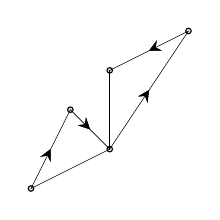
\begin{tikzpicture}[scale=0.5]
    \tkzDefPoint(0,0){v_1}
    \tkzDefPoint(1,2){v_2}
    \tkzDefPoint(2,1){v_3}
    \tkzDefPoint(4,4){v_4}
    \tkzDefPoint(2,3){v_5}
    \tkzDrawPoints(v_1,v_2,v_3,v_4,v_5)
    \tkzDrawSegments[arrowMe=stealth](v_1,v_2 v_2,v_3 v_3,v_4 v_4,v_5)
    \tkzDrawSegments(v_1,v_3 v_3,v_5)
	\end{tikzpicture}\\
	Graf posiada ścieżkę Hamiltona -- zaznaczono ją strzałkami
\end{center}
\end{minipage}
\begin{minipage}{0.5\textwidth}
\begin{center}
	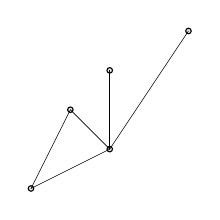
\begin{tikzpicture}[scale=0.5]
    \tkzDefPoint(0,0){v_1}
    \tkzDefPoint(1,2){v_2}
    \tkzDefPoint(2,1){v_3}
    \tkzDefPoint(4,4){v_4}
    \tkzDefPoint(2,3){v_5}
    \tkzDrawPoints(v_1,v_2,v_3,v_4,v_5)
    \tkzDrawSegments(v_1,v_2 v_2,v_3 v_3,v_4)
    \tkzDrawSegments(v_1,v_3 v_3,v_5)
	\end{tikzpicture}\\
	Graf nie posiada ścieżki Hamiltona
\end{center}
\end{minipage}


\vspace{20px}

\heading{Przykład 2}

\noindent
Zdefiniujmy ciąg grafów $(G_n)_{n\geqslant1}$ w następujący sposób.
\begin{itemize}
	\item Graf $G_1$ jest grafem złożonym z dwóch połączonych ze sobą wierzchołków,
	\item Graf $G_{i + 1}$ dla $i \geqslant 2$ otrzymujemy poprzez połączenie dwóch grafów $G_i$, aby każdy wierzchołek z jednego z tych grafów był połączony z dokładnie jednym wierzchołkiem z drugiego z tych grafów.
\end{itemize}

\noindent
Wykazać, że graf $G_{2020}$ ma ścieżkę Hamiltona.

\vspace{5px}

\begin{remark}
Można zauważyć, że $G_n$ to w istocie $n$-wymiarowy hipersześcian.
\end{remark}


\vspace{20px}

\begin{minipage}{0.33\textwidth}
\begin{center}
	\begin{tikzpicture}
    \tkzDefPoint(0,0){v_1}
    \tkzDefPoint(2,0){v_2}
    \tkzDrawPoints(v_1,v_2)
    \tkzDrawSegments(v_1,v_2)
	\end{tikzpicture}\\
	$G_1$
\end{center}
\end{minipage}
\begin{minipage}{0.33\textwidth}
\begin{center}
	\begin{tikzpicture}
    \tkzDefPoint(0,0){v_1}
    \tkzDefPoint(2,0){v_2}
    \tkzDefPoint(2,2){v_3}
    \tkzDefPoint(0,2){v_4}
    \tkzDrawPoints(v_1,v_2, v_3, v_4)
    \tkzDrawSegments(v_1,v_2 v_2,v_3 v_3,v_4 v_1,v_4)
	\end{tikzpicture}\\
	$G_2$
\end{center}
\end{minipage}
\begin{minipage}{0.33\textwidth}
\begin{center}
	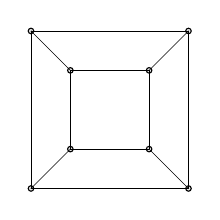
\begin{tikzpicture}
    \tkzDefPoint(0,0){v_1}
    \tkzDefPoint(2,0){v_2}
    \tkzDefPoint(2,2){v_3}
    \tkzDefPoint(0,2){v_4}
    \tkzDefPoint(0.5,0.5){v_5}
    \tkzDefPoint(1.5,0.5){v_6}
    \tkzDefPoint(1.5,1.5){v_7}
    \tkzDefPoint(0.5,1.5){v_8}
    \tkzDrawPoints(v_1,v_2, v_3, v_4)
    \tkzDrawSegments(v_1,v_2 v_2,v_3 v_3,v_4 v_1,v_4)
    \tkzDrawPoints(v_5,v_6, v_7, v_8)
    \tkzDrawSegments(v_5,v_6 v_6,v_7 v_7,v_8 v_5,v_8)
    \tkzDrawSegments(v_5,v_1 v_6,v_2 v_7,v_3 v_8,v_4)
	\end{tikzpicture}\\
	$G_3$
\end{center}
\end{minipage}

\noindent
\heading{Rozwiązanie}

\noindent
Wykażemy, że teza jest prawdziwa dla każdego $n \geqslant 1$. Co więcej wykażemy, że ścieżka Hamiltona może zaczynać się w każdym z wierzchołków $G_n$.

Zauważmy, że dla $n = 1$ teza jest oczywista -- ścieżka złożona z jednej krawędzi spełnia warunki zadania.

\vspace{10px}

\noindent
Załóżmy, że dla $G_n$ istnieje ścieżka Hamiltona. Wykażemy, że istnieje ona dla $G_{n + 1}$. Graf $G_{n+1}$ składa się z dwóch połączonych ze sobą części izomorficznych z grafem $G_n$ -- nazwijmy je $A$ oraz $B$. Oznaczmy wierzchołki $G_{n + 1}$ kolejno jako
$a_1, a_2, ..., a_{2^n}$ -- cześć $A$ oraz $b_1, b_2, ..., b_{2^n}$ -- część $B$, przy czym $a_i$ jest połączone właśnie z $b_i$. 

\vspace{10px}

\noindent
Ścieżka Hamiltonowska w grafie $G_{n + 1}$ będzie się składać z 3 części:
\begin{itemize}
	\item Na mocy założenia istnieje ścieżka zaczynająca się w $a_1$ przechodząca przez wszystkie wierzchołki $A$. Możemy ją przejść od tyłu. Wówczas przejdziemy wszystkie wierzchołki części $A$ kończąc w $a_1$.
	\item Następnie przejdziemy krawędzią między $a_1$ i $b_1$ do części $B$.
	\item Na mocy założenia z punktu $b_1$ da się poprowadzić ścieżkę, która przejdzie przez każdy z wierzchołków części $B$ dokładnie raz.
\end{itemize}

\noindent
Łatwo zauważyć, że podany sposób przejścia grafu $G_{n + 1}$ tworzy ścieżkę Hamiltonowską.

\qed

\newpage

\begin{problem}{1} 
	Wykazać, że suma miar kątów w $n$-kącie wypukłym wynosi ${(n - 2) \cdot 180\degree}$.
\end{problem}

\begin{problem}{2} 
 Wykazać, że dla każdej dodatniej liczby całkowitej $n$ zachodzi toższamość
\[
	1^2 + 2^2 + 3^2 + ... + n^2 = \frac{n(n + 1)(2n + 1)}{6}.
\]
\end{problem}

\begin{problem}{3} 
Dana jest nastepująca gra, zwana \textit{wieżami Hanoi}. Na początku ułożono $n$ dysków na jednej igle tak jak na rysunku. W każdym ruchu gracz może przemieścić dysk, wraz z wszystkimi dyskami nań leżącymy, na inną igłę, przy czym dysk ten nie może zostać położony na dysk o innej średnicy. Wykazać, że gracz jest w stanie przenieść wszystkie dyski na trzecią igłę.

\begin{center}
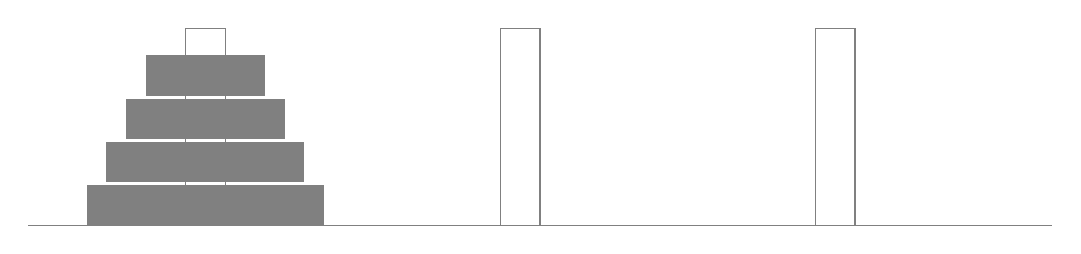
\begin{tikzpicture}[scale=0.5]
	\draw[gray, thin] (0,0) -- (26,0);
	\draw[gray, thin] (4,0) -- (4,5) -- (5,5) -- (5,0);
	\draw[gray, thin] (12,0) -- (12,5) -- (13,5) -- (13,0);
	\draw[gray, thin] (20,0) -- (20,5) -- (21,5) -- (21,0);

	\draw[gray, thin, fill=black!50] (1.5,0) -- (7.5,0) -- (7.5,1) -- (1.5,1) -- cycle;	
	\draw[gray, thin, fill=black!50] (2,1.1) -- (7,1.1) -- (7,2.1) -- (2,2.1) -- cycle;	
	\draw[gray, thin, fill=black!50] (2.5,2.2) -- (6.5,2.2) -- (6.5,3.2) -- (2.5,3.2) -- cycle;	
	\draw[gray, thin, fill=black!50] (3,3.3) -- (6,3.3) -- (6,4.3) -- (3,4.3) -- cycle;
\end{tikzpicture}

\end{center}

\end{problem}

\begin{problem}{4}
	W przestrzeni danych jest $n \geqslant 3$ punktów, że żadne trzy z nich nie leżą na jednej prostej. Każde dwa z tych punktów połączono odcinkiem o kolorze zielonym lub czerwonym. Wykazać, że można wybrać tak jeden z tych kolorów, aby każde dwa z danych punktów były połączone odcinkiem lub łamaną tego koloru.
\end{problem}

\begin{problem}{5} 
Dany jest ciąg liczb rzeczywistych
\[
	a_0 \neq 0, 1,\quad a_1 = 1 - a_0,\quad a_{n + 1} = 1 - a_n(1 - a_n). 
\]
Wykazać, że dla wszystkich $n$ 
\[
	a_1a_2...a_n\left(\frac{1}{a_1} + \frac{1}{a_2} + ... + \frac{1}{a_n}\right) = 1.
\]
\end{problem}

\newpage

\begin{problem}{6} 
	Wykazać, że planszę o wymiarach $2^n \times 2^n$ dla pewnego $n \geqslant 1$ z usuniętym jednym z rogów da się przykryć pewną liczbą $L$ klocków(takich jak na rysunku). Klocki można obracać.

	\begin{center}
		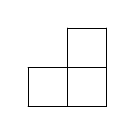
\begin{tikzpicture}[scale=0.5]
	    \tkzDefPoint(0,0){v_1}
	    \tkzDefPoint(2,0){v_2}
	    \tkzDefPoint(2,2){v_3}
	    \tkzDefPoint(1,2){v_4}
	    \tkzDefPoint(1,1){v_5}
	    \tkzDefPoint(0,1){v_6}
	    \tkzDefPoint(1,0){A}
	    \tkzDefPoint(2,1){B}

	    \tkzDrawSegments(v_1,v_2 v_2,v_3 v_3,v_4 v_4,v_5 v_5,v_6  v_6,v_1)
	    \tkzDrawSegments(v_5,A)
	    \tkzDrawSegments(v_5,B)
		\end{tikzpicture}
	\end{center}
\end{problem}

\begin{problem}{7}
Niech $n$ będzie nieparzystą liczbą naturalną, a liczby $x_1,\; x_2,\; ...,\; x_n$ będa parami różne. Dla każdych dwóch liczb $x_i$ oraz $x_j$ zapisano na tablicy wartość bezwzględną ich różnicy. Wykazać, że można podzielić zapisane liczby na dwa zbiory o równej sumie.
\end{problem}



\newpage
% Rozdział 2 – równania funkcyjne

\theory{Równania funkcyjne}

\heading{Przykład 1}

\noindent
Znajdź wszystkie funkcje $f:\mathbb{R}\rightarrow\mathbb{R}$ spełniające dla wszystkich $x, y \in \mathbb{R}$, równanie 
\[
    f(x + y) = f(x) − f(y).
\]

\heading{Rozwiązanie}

\noindent
Zauważmy, że skoro dane równanie jest spełnione dla wszystkich liczb rzeczywistych $x$~i~$y$ to jest spełnione w szczególności dla $x = y = 0$. Wówczas
\begin{gather*}
    f(0) = f(0) - f(0) = 0.
\end{gather*}

\noindent
Podstawiając do wyjściowej równości $x = 0$ otrzymujemy
\[
    f(y) = f(0) - f(y).
\]
Na mocy wyżej wykazanej zależności $f(y) = 0$ mamy
\begin{gather*}
    f(y) = - f(y) \\
    f(y) = 0.
\end{gather*}
Wykazaliśmy, że $f(x) = 0$ dla wszystkich liczb rzeczywistych $x$. Pozostaje sprawdzić, że istotnie taka funkcja spełnia warunki zadania. Zauważmy, że wówczas
\[
    f(x + y) = 0 = f(x) - f(y).
\]

\qed

\vspace{10px}

\noindent
Metodę, polegająca na podstawianiu szczególnych wartości do danego równania, jest najważniejszym narzędziem w walce z równaniami funkcyjnymi. Często, aby zadania rozwiązać, należy użyć jej kilka lub nawet kilkanaście razy.

\vspace{10px}

\noindent
Należy zaznaczyć, że bardzo często rozwiązując równanie funkcyjne, wyznacza się zbiór funkcji, które mogą spełniać dane równanie. Jednak często nie oznacza to, że muszą one go spełniać, gdyż podstawianie zazwyczaj nie jest przejściem równoważnym. Dlatego należy zawsze w swoim rozwiązaniu zawrzeć sprawdzenie tego, czy otrzymane funkcje istotnie działają. Brak takiego sprawdzenie w większości przypadków skutkuje obniżeniem oceny za dane zadanie.

\vspace{20px}

\heading{Przykład 2}

\noindent
Znajdź wszystkie funkcje $f:\mathbb{R}\rightarrow\mathbb{R}$ spełniające dla wszystkich $x, y \in \mathbb{R}$ równanie 
\[
    f(2f(x) + f(y)) = 2x + f(y).
\]

\newpage

\heading{Rozwiązanie}

\noindent
Rozwiązanie rozpoczniemy od wykazania następującego lematu.

\vspace{10px}

\noindent
\underline{Lemat 1.} Dla każdego $a \in \mathbb{R}$ istnieje $x \in \mathbb{R}$, że $f(x) = a$.

\vspace{5px}

\noindent
Podstawmy $\dfrac{a - f(y)}{2}$ w miejsce zmiennej $x$
\[
    f\left(f\left(\frac{a - f(y)}{2}\right) + f(y)\right) = 2\left(\frac{a - f(y)}{2}\right) + f(y) = a.
\]

\noindent
Zauważmy, że z otrzymanej równości wynika teza lematu – liczbę $a$ można wybrać dowolnie, zaś po prawej stronie otrzymamy argument, dla którego funkcja przyjmie tę wartość.

\vspace{10px}

\noindent
Korzystając z lematu, podstawmy w miejsce $y$ taką liczbę $a$, aby $f(a) = -2f(x)$. Wówczas
\begin{gather*}
    f(2f(x) + f(a)) = 2x + f(a) \\
     f(0) = 2x - 2f(x) \\
    f(x) = x  + \frac{1}{2}f(0).
\end{gather*}
Podstawiając do powyższej równości $x = 0$ otrzymujemy, że $f(0) = 0$. Stąd
\[
    f(x) = x + \frac{1}{2}f(0) = x.
\]
Sprawdzamy, że funkcja $f(x) = x$ istotnie spełnia warunki zadania.

\qed

\vspace{10px}

\noindent
W powyższym rozumowaniu kluczowe było wykazanie, że dana funkcja przyjmuje wszystkie wartości rzeczywiste -- inaczej mówiąc jest surjekcją. Mogliśmy także wykazać więcej, mianowicie, że dana funkcja jest różnowartościowa. Zakładając, że $f(a) = f(b)$ dla pewnych liczb $a,\;b$ podstawiamy w miejsce $(x, y)$ kolejno $(a, 0)$ i $(b, 0)$ otrzymując
\[
    f(2f(a) + f(y)) = 2a + f(y) \quad \text{oraz} \quad f(2f(b) + f(y)) = 2b + f(y).
\]
Na mocy wyżej założonej równości lewe strony obu zależności są sobie równe. Stąd prawe również, skąd $a = b$. Implikacja $f(a) = f(b) \implies a = b$ jest równoważna temu, że funkcja~$f$ jest różnowartościowa.

\vspace{10px}

\noindent
W większości rozwiązań funkcyjnych konieczne będzie wykonanie wielu ,,sztampowych'' podstawień i spróbować wykazać własności funkcji -- chociażby te wspomniane wyżej. Niekiedy do rozwiązania zadania potrzebny będzie błyskotliwy pomysł czy nietypowe połączenie faktów. W innych zaś przypadkach samo rzetelne i uważne próbowanie znanych trików może okazać się wystarczające. 

\vspace{10px}

\begin{problem}{1} 
	Znajdź wszystkie funkcje $\mathbb{R} \rightarrow \mathbb{R} $ spełniające dla wszystkich $x, y \in \mathbb{R} $ równanie
	\[
		 f(x)+f(y) = f(xy).
	\]
\end{problem}

\begin{problem}{2}
	Znajdź wszystkie funkcje $\mathbb{R} \rightarrow \mathbb{R} $ spełniające dla wszystkich $x, y \in \mathbb{R} $ równanie
	\[
		 f(x-f(y)) = 1 - x - y.
	\]
\end{problem}

\begin{problem}{3}
	Znajdź wszystkie funkcje $\mathbb{R} \rightarrow \mathbb{R} $ spełniające dla wszystkich $x, y \in \mathbb{R} $ równanie 
	\[
		f(x^{2}y) = f(xy) + yf(f(x) + y).
	\]
\end{problem}

\begin{problem}{4}
	Znajdź wszystkie funkcje $\mathbb{R} \rightarrow \mathbb{R} $ spełniające dla wszystkich $x, y \in \mathbb{R} $ równanie 
	\[
		2f(x) + f(1 - x) = x^{2}.
	\] 
\end{problem}

\begin{problem}{5}
	Znajdź wszystkie funkcje $\mathbb{R} \rightarrow \mathbb{R} $ spełniające dla wszystkich $x, y \in \mathbb{R} $ równanie 
	\[
		f(x+y) = f(f(x)) + y + 1.
	\] 
\end{problem}

\begin{problem}{6}
	Znajdź wszystkie funkcje różnowartościowe
	$\mathbb{R} \rightarrow \mathbb{R} $ spełniające dla wszystkich $x, y \in \mathbb{R} $ równość 
	\[
		f(f(x) + y) = f(x+y) + 1.
	\]
\end{problem}

\begin{problem}{7}
	Znajdź wszystkie funkcje 
	$\mathbb{R} \rightarrow \mathbb{R} $ spełniające dla wszystkich $x, y \in \mathbb{R} $ nierówność 
	\[
		f(x^2+y) + f(y) \geqslant f(x^2) + f(x).
	\] 
\end{problem}

\begin{problem}{8}
	Znajdź wszystkie funkcje $\mathbb{Z} \rightarrow \mathbb{Z} $ spełniające dla wszystkich $x \in \mathbb{Z} $ równanie
	\[
		 f(f(x)) =x+1.
	\] 
\end{problem}

\begin{problem}{9}
	Znajdź wszystkie funkcje $\mathbb{R} \rightarrow \mathbb{R} $ spełniające dla wszystkich $x, y \in \mathbb{R} $ równanie 
	\[
		f(x) f(y) = f(x-y).
	\] 
\end{problem}

\begin{problem}{10}
	Udowodnij, że nie istnieje taka funkcja $f:\mathbb{R}\longrightarrow\mathbb{R}$, że dla dowolnych liczb rzeczywistych $x$, $y$ zachodzi równość:
	\[
		f(f(x) + 2f(y)) = x + y.
	\]
\end{problem}



\newpage
% Rozdział 3 – Bijekcje i bajki kombinatoryczne

\theory{Bijekcje i bajki kombinatoryczne}

\noindent
W tym rozdziale będziemy analizować różne zbiory i relacje między nimi. W części zadań trzeba będzie pokazać, że pewne dwa zbiory mają tyle samo elementów. Jedną z metod dowodzenia tego typu stwierdzeń jest połączenie elementów danych zbiorów w pary. Takie przyporządkowanie nazywamy \textit{bijekcją}.

\begin{center}
    \begin{tikzpicture}
        \tkzDefPoint(-1,3){P_0}
        \tkzDefPoint(0,3){P_1}
        \tkzDefPoint(1,3){P_2}
        \tkzDefPoint(2,3){P_3}
        \tkzDefPoint(3,3){P_4}
        \tkzDefPoint(4,3){P_5}
        \tkzDefPoint(5,3){P_6}


        \tkzDefPoint(-1,1){Q_0}
        \tkzDefPoint(0,1){Q_1}
        \tkzDefPoint(1,1){Q_2}
        \tkzDefPoint(2,1){Q_3}
        \tkzDefPoint(3,1){Q_4}
        \tkzDefPoint(4,1){Q_5}
        \tkzDefPoint(5,1){Q_6}

        \tkzDrawSegments[dashed](P_1,Q_1 P_2,Q_2 P_3,Q_3 P_4,Q_4 P_5,Q_5 P_6,Q_6)

        \tkzDrawPoints(P_1, P_2, P_3, P_4, Q_1, Q_2, Q_3, Q_4, P_5, P_6, Q_5, Q_6)

        \tkzLabelPoint[left](P_0){Zbiór $A$}
        \tkzLabelPoint[left](Q_0){Zbiór $B$}
    \end{tikzpicture}
\end{center}

\vspace{10px}

\noindent
Aby stwierdzić czy przyporządkowanie jest bijekcją, wystarczy sprawdzić czy każdy element jednego zbioru jest przyporządkowany do \textit{dokładnie} jednego elementu drugiego zbioru. Poniżej dwa przykłady przyporządkowań, które nie są bijekcjami.

\begin{center}
    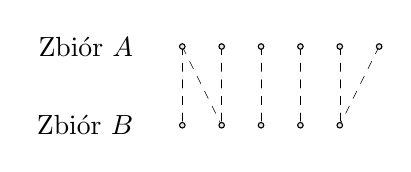
\begin{tikzpicture}[scale=0.5]
        \tkzDefPoint(-1,3){P_0}
        \tkzDefPoint(0,3){P_1}
        \tkzDefPoint(1,3){P_2}
        \tkzDefPoint(2,3){P_3}
        \tkzDefPoint(3,3){P_4}
        \tkzDefPoint(4,3){P_5}
        \tkzDefPoint(5,3){P_6}


        \tkzDefPoint(-1,1){Q_0}
        \tkzDefPoint(0,1){Q_1}
        \tkzDefPoint(1,1){Q_2}
        \tkzDefPoint(2,1){Q_3}
        \tkzDefPoint(3,1){Q_4}
        \tkzDefPoint(4,1){Q_5}
        \tkzDefPoint(5,1){Q_6}

        \tkzDrawSegments[dashed](P_1,Q_1 P_2,Q_2 P_3,Q_3 P_4,Q_4 P_5,Q_5 P_6,Q_5 P_1,Q_2)

        \tkzDrawPoints(P_1, P_2, P_3, P_4, Q_1, Q_2, Q_3, Q_4, P_5, P_6, Q_5)

        \tkzLabelPoint[left](P_0){Zbiór $A$}
        \tkzLabelPoint[left](Q_0){Zbiór $B$}
    \end{tikzpicture}
    \hspace{20px}
    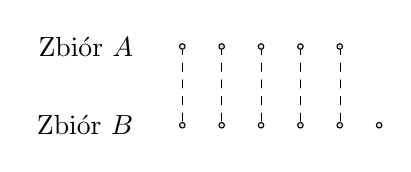
\begin{tikzpicture}[scale=0.5]
        \tkzDefPoint(-1,3){P_0}
        \tkzDefPoint(0,3){P_1}
        \tkzDefPoint(1,3){P_2}
        \tkzDefPoint(2,3){P_3}
        \tkzDefPoint(3,3){P_4}
        \tkzDefPoint(4,3){P_5}
        \tkzDefPoint(5,3){P_6}


        \tkzDefPoint(-1,1){Q_0}
        \tkzDefPoint(0,1){Q_1}
        \tkzDefPoint(1,1){Q_2}
        \tkzDefPoint(2,1){Q_3}
        \tkzDefPoint(3,1){Q_4}
        \tkzDefPoint(4,1){Q_5}
        \tkzDefPoint(5,1){Q_6}

        \tkzDrawSegments[dashed](P_1,Q_1 P_2,Q_2 P_3,Q_3 P_4,Q_4 P_5,Q_5)

        \tkzDrawPoints(P_1, P_2, P_3, P_4, Q_1, Q_2, Q_3, Q_4, P_5, Q_5, Q_6)

        \tkzLabelPoint[left](P_0){Zbiór $A$}
        \tkzLabelPoint[left](Q_0){Zbiór $B$}
    \end{tikzpicture}
\end{center}

\heading{Przykład 1}

\noindent
Dla pewnej liczby całkowitej $n$ jej \textit{podziałem} nazwiemy takie dodatnie liczby całkowite $(a_1, ..., a_t)$, że
\begin{gather*}
    n = a_1 + a_2 + ... + a_t \\
    a_1 \geqslant a_2 \geqslant a_3 \geqslant ... \geqslant a_t \geqslant 0.
\end{gather*}

\noindent
Niech $n$, $k$ będą dodatnimi liczbami całkowitymi. Wykazać, że liczba podziałów $n$, które składają się dokładnie z $k$ liczb jest równa liczbie podziałów $n$, takich, że największy składnik każdego z nich jest równy dokładnie $k$.

\vspace{5px}

\heading{Rozwiązanie}

\vspace{5px}

\noindent
Weźmy dowolny podział liczby $n$. Niech $n = a_1 + a_2 + ... + a_t$. Rozpatrzmy jego reprezentację graficzną zwaną diagramem Ferrera.
Poniżej narysowano diagram Ferrera dla podziału $12 = 4 + 4 + 3 + 1$.
W każdym kolejnym wierszu znajduje się tyle kropek, ile wynosi kolejny składnik z podziału. 

\begin{center}
    \begin{tikzpicture}[scale=0.6]

        \tkzDefPoint(-1,3){A_1}
        \tkzDefPoint(0,3){P_1}
        \tkzDefPoint(1,3){P_2}
        \tkzDefPoint(2,3){P_3}
        \tkzDefPoint(3,3){P_4}


        \tkzDefPoint(-1,2){A_2}
        \tkzDefPoint(0,2){P_5}
        \tkzDefPoint(1,2){P_6}
        \tkzDefPoint(2,2){P_7}
        \tkzDefPoint(3,2){P_8}

        \tkzDefPoint(-1,1){A_3}
        \tkzDefPoint(0,1){P_9}
        \tkzDefPoint(1,1){P_10}
        \tkzDefPoint(2,1){P_11}

        \tkzDefPoint(-1,0){A_4}
        \tkzDefPoint(0,0){P_12}

        \tkzDrawPoints(P_1, P_2, P_3, P_4, P_5, P_6, P_7, P_8, P_9, P_10, P_11, P_12)
        \tkzLabelPoint[left](A_1){4}
        \tkzLabelPoint[left](A_2){4}
        \tkzLabelPoint[left](A_3){3}
        \tkzLabelPoint[left](A_4){1}

        \tkzDefPoint(0,4){B_1}
        \tkzDefPoint(1,4){B_2}
        \tkzDefPoint(2,4){B_3}
        \tkzDefPoint(3,4){B_4}
        \tkzLabelPoint[above](B_1){4}
        \tkzLabelPoint[above](B_2){3}
        \tkzLabelPoint[above](B_3){3}
        \tkzLabelPoint[above](B_4){2}
    \end{tikzpicture}
\end{center}

\noindent
Zastanówmy się, co znaczą założenia zadania w języku rozpatrywanych diagramów.
Jeśli w podziale jest dokładnie $k$ liczb, to diagram Ferrera będzie składał się dokładnie z $k$ wierszy. Jeśli  największy składnik podziału jest równy $k$, to kolumn będzie dokładnie $k$.

\vspace{10px}
\noindent
Zauważmy, że patrząc na dowolny diagram Ferrera ,,od góry'' -- traktujemy kolumny jako wiersze i vice versa -- otrzymamy inny diagram Ferrera. W podanym przykładzie z podziału $12 = 4 + 4 + 3 + 1$ otrzymamy w ten sposób podział $12 = 4 + 3 + 3 + 2$.

\vspace{10px}
\noindent
Jeśli diagram Ferrera przedstawiał podział $n$, który składa się dokładnie z $k$ liczb, to podział otrzymany w powyższy sposób ma największy składnik każdego z nich równy dokładnie $k$. Obie z tych własności są równoważne temu, że diagram na $k$ wierszy.

\vspace{10px}
\noindent
Powyższe przyporządkowanie łączy elementy danych w zadaniu zbiorów w pary -- dokładnie jeden podział pierwszego rodzaju z dokładnie jednym podziałem drugiego rodzaju. Rysując diagram dla pewnego podziału, otrzymamy dokładnie jeden podział z drugiego zbioru, więc to parowanie jest dobre. Stąd wynika, że rozpatrywane zbiory mają tyle samo elementów.

\qed

\vspace{10px}

\noindent
Pokazaliśmy, że pewne dwa zbiory mają tę samą liczbę elementów. Teraz spróbujemy za pomocą kombinatoryki udowodnić równość algebraiczną.

\vspace{5px}


\heading{Przykład 2}

\noindent
Wykazać, że dla wszystkich dodatnich liczb całkowitych $n$, $k$ zachodzi równość
\[
    \sum^{n}_{k=0} {{n}\choose{k}} 2^k = 3^n.
\]

\vspace{5px}

\heading{Rozwiązanie}

\vspace{5px}

\noindent
Na imprezę przyszło $n$ matematyczek. Każda z nich wzięła kapelusz, czapkę lub przyszła bez okrycia głowy. Obliczmy ile różnych wariantów nakryć głowy mogło się zdarzyć na dwa sposoby.
\begin{enumerate}
    \item Każda z dziewczyn mogła wybrać jedną z trzech opcji ubioru, było ich $n$, więc liczba możliwości wynosi $3^n$.
    \item Przyjmijmy, że $n - k$ dziewczyn nie przyniosło żadnego nakrycia głowy. 
    Wówczas możemy wybrać te dziewczyny na ${{n}\choose{n - k}} = {{n}\choose{k}}$ sposobów. 
    Następnie każda z pozostałych $k$ dziewczyn wybrała jedno z dwóch dostępnych nakryć głowy. 
    Więc mogą to zrobić na $2^k$ sposobów. Z reguły mnożenia wynika, że dla ustalonej liczby $k$ jest dokładnie ${{n}\choose{k}} 2^k$ wariantów. Sumując po wszystkich $k$ otrzymujemy $\sum^{n}_{k=0} {{n}\choose{k}} 2^k$.
\end{enumerate}

\noindent
Obliczając jedną rzecz na dwa sposoby otrzymaliśmy liczby, które muszą być równe.

\qed

\vspace{10px}

\noindent
Rozumowania podobne do powyższego nazywane są bajkami kombinatorycznymi.

\vspace{10px}
\begin{problem}{1} 
	Znajdź wszystkie funkcje $\mathbb{R} \rightarrow \mathbb{R} $ spełniające dla wszystkich $x, y \in \mathbb{R} $ równanie
	\[
		 f(x)+f(y) = f(xy).
	\]
\end{problem}

\begin{problem}{2}
	Znajdź wszystkie funkcje $\mathbb{R} \rightarrow \mathbb{R} $ spełniające dla wszystkich $x, y \in \mathbb{R} $ równanie
	\[
		 f(x-f(y)) = 1 - x - y.
	\]
\end{problem}

\begin{problem}{3}
	Znajdź wszystkie funkcje $\mathbb{R} \rightarrow \mathbb{R} $ spełniające dla wszystkich $x, y \in \mathbb{R} $ równanie 
	\[
		f(x^{2}y) = f(xy) + yf(f(x) + y).
	\]
\end{problem}

\begin{problem}{4}
	Znajdź wszystkie funkcje $\mathbb{R} \rightarrow \mathbb{R} $ spełniające dla wszystkich $x, y \in \mathbb{R} $ równanie 
	\[
		2f(x) + f(1 - x) = x^{2}.
	\] 
\end{problem}

\begin{problem}{5}
	Znajdź wszystkie funkcje $\mathbb{R} \rightarrow \mathbb{R} $ spełniające dla wszystkich $x, y \in \mathbb{R} $ równanie 
	\[
		f(x+y) = f(f(x)) + y + 1.
	\] 
\end{problem}

\begin{problem}{6}
	Znajdź wszystkie funkcje różnowartościowe
	$\mathbb{R} \rightarrow \mathbb{R} $ spełniające dla wszystkich $x, y \in \mathbb{R} $ równość 
	\[
		f(f(x) + y) = f(x+y) + 1.
	\]
\end{problem}

\begin{problem}{7}
	Znajdź wszystkie funkcje 
	$\mathbb{R} \rightarrow \mathbb{R} $ spełniające dla wszystkich $x, y \in \mathbb{R} $ nierówność 
	\[
		f(x^2+y) + f(y) \geqslant f(x^2) + f(x).
	\] 
\end{problem}

\begin{problem}{8}
	Znajdź wszystkie funkcje $\mathbb{Z} \rightarrow \mathbb{Z} $ spełniające dla wszystkich $x \in \mathbb{Z} $ równanie
	\[
		 f(f(x)) =x+1.
	\] 
\end{problem}

\begin{problem}{9}
	Znajdź wszystkie funkcje $\mathbb{R} \rightarrow \mathbb{R} $ spełniające dla wszystkich $x, y \in \mathbb{R} $ równanie 
	\[
		f(x) f(y) = f(x-y).
	\] 
\end{problem}

\begin{problem}{10}
	Udowodnij, że nie istnieje taka funkcja $f:\mathbb{R}\longrightarrow\mathbb{R}$, że dla dowolnych liczb rzeczywistych $x$, $y$ zachodzi równość:
	\[
		f(f(x) + 2f(y)) = x + y.
	\]
\end{problem}



\newpage
% Rozdział 4 – liczby pierwsze i reszty z dzielenia



\theory{Liczby pierwsze i reszty z dzielenia}

\noindent
Ten rozdział będzie nieco bardziej teoretyczny niż poprzednie. Zadania także będą trudniejsze -- zachęcamy do skorzystania ze wskazówek i głębokiego przestudiowania rozwiązań. Chcemy wyrobić u czytelnika intuicję dotyczącą działań na resztach z dzielenia przez pewną liczbę pierwszą. Od czytelniczki/czytelnika wymaga się, aby znał własności kongruencji -- opisano je chociażby w  \href{https://omj.edu.pl/uploads/attachments/kwadrat-07-kolor.pdf}{Gazetce OMJ ,,Kwadrat'' nr 7}. 

\vspace{5px}

\noindent
We wszystkich poniższych zadaniach przez $a$, $b$ będziemy oznaczać liczby całkowite, zaś przez $p$ dowolną liczbę pierwszą. Przez $x \big| y$ będziemy oznaczać fakt, że liczba $x$ jest dzielnikiem liczby $y$.

\vspace{5px}
\heading{Twierdzenie 1}

\noindent
Jeśli liczba $ab$ jest podzielna przez $p$, to wówczas co najmniej jedna z liczb $a$, $b$ jest podzielna przez $p$.

\vspace{15px}

\noindent
Zauważmy, że założenie o pierwszości liczby $p$ jest konieczne. Chociażby liczba $4 \cdot 9 = 36$ dzieli się przez $6$, ale żadna z liczb $4$, $9$ nie jest podzielna przez $6$.

\vspace{5px}
\noindent
Zachęcamy do samodzielnej próby wykazania poniższych lematów. Poniżej, czcionką odwróconą, zapisano wskazówki.

\vspace{5px}
\heading{Lemat 1}

\noindent
Udowodnić, że jeśli $x^2\equiv 1 \pmod{p}$ dla pewnej liczby pierwszej $p$, to \[   
    x\equiv 1 \pmod{p} \quad \text{lub} \quad x\equiv -1 \pmod{p}.
\]

\rotatehint{Zapisz założenia i tezę zadania bez użycia modulo.}

\heading{Dowód}

\noindent
Zauważamy, że zapis $x^2\equiv 1 \pmod{p}$ jest równoważny zapisowi 
\[
    p \mid x^2-1=(x-1)(x+1).
\]
 Skoro $p$ jest liczbą pierwszą, to na mocy Twierdzenia 1 zachodzi $p\mid x-1$ lub $p\mid x+1$, a to jest równoważne temu, co było do wykazania.
 
\qed

\vspace{10px}

\heading{Lemat 2}

\noindent
Liczba $a$ nie jest podzielna przez $p$. Udowodnić, że istnieje taka dodatnia liczba całkowita~$k$, że 
\[
   a^k\equiv 1 \pmod{p}.
\]

\rotatehint{Udowodnij, że istnieją takie $r$ i $s$, że $a^r\equiv a^s \pmod{p}$.}

\heading{Dowód}

\noindent
Rozpatrzmy ciąg $(1,\; a^1,\; a^2,\; a^3,\; ...)$ . Zauważamy, że ma on nieskończenie wiele elementów, a reszt z dzielenia przez $p$ jest skończenie wiele. Z Zasady Szufladkowej Dirichleta mamy więc, że istnieją takie liczby $r$ oraz $s$ -- załóżmy, że $r\geqslant s $ -- że 
\[
    a^r\equiv a^s \pmod{p}.
\]
Jest to równoważne temu, że 
\[  
    p\mid a^s(a^{r-s}-1).
\]
Skoro $a$ nie jest podzielna przez $p$, to $p\mid a^{r-s}-1$, skąd zachodzi $a^{r-s}\equiv 1 \pmod{p}$.

\qed


\vspace{10 px}
\heading{Odwrotności modulo p}

\noindent
Z Lematu 2 można wywnioskować, że dla każdej liczby $a$, która nie jest podzielna przez $p$ istnieje pewna liczba $b \in \{1, 2, ..., p-1\}$, że
\[
    ab \equiv 1 \pmod{p}.
\]
Wystarczy wziąć $b = a^{k - 1} \text{ mod } p$. 

\vspace{10px}
\noindent
Wykażemy teraz, że w zbiorze $\{1, 2, ..., p-1\}$ jest dokładnie jedna taka liczba $b$. Załóżmy, że dla pewnych $b, c \in \{1, 2, ..., p-1\}$
\[
    ab \equiv  ac \equiv 1 \pmod{p}.
\]
Wówczas
\[
    p \big| ab - ac = a(b - c) \implies p \big|b - c,
\]
gdyż liczba $a$ nie jest podzielna przez $p$. Skoro $b, c \in \{1, 2, ..., p-1\}$, to 
\[
    - p < b - c < p.
\]
Skoro $p \big| b - c$, to $b - c = 0$, czyli $b = c$.

\vspace{10px}

\noindent
Przyjmiemy, że liczba $b$ jest \textit{odwrotnością} liczby $a$ modulo $p$. Zapiszemy $b = a^{-1} \pmod{p}$.

\vspace{10px}

\heading{Lemat 3}

\noindent
Dla dowolnej liczby $a$, która nie jest podzielna przez $p$ ciąg
\[
    (a \text{ (mod } p),\;\; 2a \text{ (mod } p),\;\;  3a \text{ (mod } p), ...,\;\;  (p - 1) \cdot a \text{ (mod } p))
\]
jest permutacją ciągu
\[
 (1,\; 2,\; 3,\; ...,\; p - 1).
\]

\rotatehint{Wykaż, że $ai \not\equiv aj \pmod{p}$, jeśli $i \not\equiv j \pmod{p}$.}

\heading{Dowód}

\noindent
Pokażmy, że jeśli $i \not\equiv j \pmod{p}$, to $ai \not\equiv aj \pmod{p}$. 
Załóżmy, że 
\[
    ai \equiv aj \pmod{p}
\] 
dla pewnych $i,\; j$. Skoro $p$ nie dzieli $a$, to istnieje odwrotność $a$ modulo $p$. Mnożąc obie strony przez $a^{-1}$ -- lub równoważnie dzieląc przez $a$ otrzymujemy
\[
    i \equiv j \pmod{p},
\]
co dowodzi postulowanej implikacji.

\vspace{10px}
\noindent
Rozpatrzmy liczby $a, \; 2a,\; (p - 1)a$. Oczywiście żadna z nich nie jest podzielna przez~$p$. Z tego, że tych liczb jest $p - 1$, niezerowych reszt z dzielenia przez $p$ również jest $p - 1$, oraz te liczby dają parami różne reszty niezerowe z dzielenia przez $p$, wynika teza.

\qed


\newpage

\heading{Małe twierdzenie Fermata}

\noindent
Dana jest liczba $a$, która nie jest podzielna przez $p$. Wykazać, że
\[
    a^{p - 1} \equiv 1 \pmod{p}.
\]

\heading{Dowód}

\noindent
Korzystając z poprzedniego lematu mamy, że ciąg
\[
    (a \text{ (mod } p),\;\; 2a \text{ (mod } p),\;\;  3a \text{ (mod } p), ...,\;\;  (p - 1) \cdot a \text{ (mod } p))
\]
jest permutacją ciągu
\[
 (1,\; 2,\; 3,\; ...,\; p - 1).
\]
Skoro te ciągi zawierają te same elementy modulo $p$, tylko, że w innej kolejności, to iloczyny tych elementów będą dawały taką samą resztę z dzielenie przez $p$. Więc
\[
    1 \cdot 2 \cdot 3 \cdot ... \cdot (p - 1) = a \cdot 2a \cdot 3a \cdot ... \cdot (p - 1)a \pmod{p},
\]
\[
    (p - 1)! \equiv a^{p - 1}(p - 1)! \pmod{p}.
\]
Zauważmy, że $(p - 1)! \not\equiv 0 \pmod{p}$. Mnożać przystawanie stronami przez odwrotność liczby~$(p - 1)!$ otrzymujemy tezę.

\qed

\vspace{10px}

\begin{problem}{1} 
	Znajdź wszystkie funkcje $\mathbb{R} \rightarrow \mathbb{R} $ spełniające dla wszystkich $x, y \in \mathbb{R} $ równanie
	\[
		 f(x)+f(y) = f(xy).
	\]
\end{problem}

\begin{problem}{2}
	Znajdź wszystkie funkcje $\mathbb{R} \rightarrow \mathbb{R} $ spełniające dla wszystkich $x, y \in \mathbb{R} $ równanie
	\[
		 f(x-f(y)) = 1 - x - y.
	\]
\end{problem}

\begin{problem}{3}
	Znajdź wszystkie funkcje $\mathbb{R} \rightarrow \mathbb{R} $ spełniające dla wszystkich $x, y \in \mathbb{R} $ równanie 
	\[
		f(x^{2}y) = f(xy) + yf(f(x) + y).
	\]
\end{problem}

\begin{problem}{4}
	Znajdź wszystkie funkcje $\mathbb{R} \rightarrow \mathbb{R} $ spełniające dla wszystkich $x, y \in \mathbb{R} $ równanie 
	\[
		2f(x) + f(1 - x) = x^{2}.
	\] 
\end{problem}

\begin{problem}{5}
	Znajdź wszystkie funkcje $\mathbb{R} \rightarrow \mathbb{R} $ spełniające dla wszystkich $x, y \in \mathbb{R} $ równanie 
	\[
		f(x+y) = f(f(x)) + y + 1.
	\] 
\end{problem}

\begin{problem}{6}
	Znajdź wszystkie funkcje różnowartościowe
	$\mathbb{R} \rightarrow \mathbb{R} $ spełniające dla wszystkich $x, y \in \mathbb{R} $ równość 
	\[
		f(f(x) + y) = f(x+y) + 1.
	\]
\end{problem}

\begin{problem}{7}
	Znajdź wszystkie funkcje 
	$\mathbb{R} \rightarrow \mathbb{R} $ spełniające dla wszystkich $x, y \in \mathbb{R} $ nierówność 
	\[
		f(x^2+y) + f(y) \geqslant f(x^2) + f(x).
	\] 
\end{problem}

\begin{problem}{8}
	Znajdź wszystkie funkcje $\mathbb{Z} \rightarrow \mathbb{Z} $ spełniające dla wszystkich $x \in \mathbb{Z} $ równanie
	\[
		 f(f(x)) =x+1.
	\] 
\end{problem}

\begin{problem}{9}
	Znajdź wszystkie funkcje $\mathbb{R} \rightarrow \mathbb{R} $ spełniające dla wszystkich $x, y \in \mathbb{R} $ równanie 
	\[
		f(x) f(y) = f(x-y).
	\] 
\end{problem}

\begin{problem}{10}
	Udowodnij, że nie istnieje taka funkcja $f:\mathbb{R}\longrightarrow\mathbb{R}$, że dla dowolnych liczb rzeczywistych $x$, $y$ zachodzi równość:
	\[
		f(f(x) + 2f(y)) = x + y.
	\]
\end{problem}



\newpage
% Rozdział 5 – nierówności między średnimi
% dowód AM-GM dla wielu zmiennych
% pokazanie jakiegoś szacowania, uwaga o przejściu z równością
% inne szacowanie z szacowaniem częściowym

\theory{Nierówności między średnimi}

\noindent
Zakładamy, że czytelniczka/czytelnik zna metodę dowodzenia nierówności poprzez zwinięcie do kwadratu. Zaprezentujemy jedno twierdzenie -- nierówność między średnimi -- oraz kilka metod pracy z nierównoścami.

\vspace{10px}

\heading{Nierówności między średnimi}

\noindent
Dane są dodatnie liczby rzeczywiste $a_1,\; a_2, \; a_3, \; ..., \; a_n$.

\noindent
Średnią kwadratową nazywamy wartość
\[
    QM = \sqrt{\frac{a_1^2 + a_2^2 + ... + a_n^2}{n}}.
\]
Średnią arytmetyczną nazywamy wartość
\[
    AM = \frac{a_1 + a_2 + ... + a_n}{n}.
\]
Średnią geometryczną nazywamy wartość
\[
    GM = \sqrt[n]{a_1a_2...a_n}.
\]
Średnią harmoniczną nazywamy wartość
\[
   HM = \frac{n}{\frac{1}{a_1} + \frac{1}{a_2} + ... + \frac{1}{a_n}}.
\]

\noindent
Wówczas zachodzą nierówności
\[
    QM \geqslant AM \geqslant GM \geqslant HM,
\]
przy czym równość w którymkolwiek przypadku zachodzi wtedy i tylko wtedy, gdy
\[
    a_1 = a_2 = ... = a_n.
\]

\vspace{10px}
\noindent
Skróty $QM$, $AM$, $GM$, $HM$ pochodzą z języka angielskiego i oznaczają odpowiednio \textit{quadratic mean}, \textit{arithmetic mean}, \textit{geometric mean}, \textit{harmonic mean}. Zaprezentujemy dowód jednej z podanych nierówności. Pozostałe są nieco bardziej złożone, więc nie będziemy ich przytaczać.

\vspace{10px}

\heading{Dowód nierówności między średnimi arytmetyczną a geometryczną}

\noindent
\underline{Cześć 1.} Dowód $n = 2$.

\vspace{10px}

\noindent
Chcemy wykazać, że zachodzi nierówność
\[
    \frac{a_1 + a_2}{2} \geqslant \sqrt{a_1a_2}.
\]
Jest ona równoważna prawdziwej nierówności
\[
    a_1 - 2\sqrt{a_1a_2} + a_2 = (\sqrt{a_1} - \sqrt{a_2})^2 \geqslant 0.
\]

\noindent
\underline{Cześć 2.} Dowód dla $n$ postaci $n = 2^k$, $k \in \mathbb{Z}_{\geqslant 0}$.

\vspace{10px}

\noindent
Będziemy indukować się po $k$. Dla $k = 0$ nierówność jest oczywista. Załóżmy, że zachodzi dla $k$, wykażemy, że zachodzi dla $k + 1$.

\noindent
Zauważmy, że
\[
    \frac{a_1 + a_2 + ... + a_{2^{k + 1}}}{2^{k + 1}} = \frac{1}{2}\left( \frac{a_1 + a_2 + ... + a_{2^{k}}}{2^{k}} + \frac{a_{2^k + 1} + a_{2^k + 2} + ... + a_{2^{k + 1}}}{2^{k}}\right)
\]

\noindent
Korzystając z założenia indukcyjnego -- to jest nierówności dla $n = 2^{k}$ mamy
\begin{align*}
    \frac{a_1 + a_2 + ... + a_{2^{k}}}{2^{k}} &\geqslant \sqrt[2^k]{a_1a_2...a_{2^k}} \\
   \frac{a_{2^k + 1} + a_{2^k + 2} + ... + a_{2^{k + 1}}}{2^{k}} &\geqslant \sqrt[2^k]{a_{2^k + 1}a_{2^k + 2}...a_{2^{k + 1}}}
\end{align*}

\noindent
Zauważmy teraz, że na mocy znanej nierówności $a + b \geqslant 2\sqrt{ab}$ mamy
\[
    \frac{1}{2}\left(\sqrt[2^k]{a_1a_2...a_{2^k}} + \sqrt[2^k]{a_{2^k + 1}a_{2^k + 2}...a_{2^{k + 1}}}\right) \geqslant \sqrt[2^{k + 1}]{a_1a_2...a_{2^{k + 1}}}
\]
Łącząc powyższe nierówności, otrzymujemy dowód nierówności dla $n$ będącej potęgą liczby $2$.

\vspace{10px}

\noindent
\underline{Cześć 3.} Z faktu, że nierówność zachodzi dla $n \geqslant 2$ wynika, że zachodzi dla $n - 1$.

\vspace{10px}

\noindent
Oznaczmy 
\[
    AM = \frac{a_1 + a_2 + ... + a_{n - 1}}{n - 1} \quad \text{oraz} \quad GM = \sqrt[n - 1]{a_1a_2...a_{n - 1}}.
\]

\noindent
Skoro nierówność zachodzi dla liczby $n$ to mamy
\[
    AM = \frac{(n-1)AM + AM}{n} = \frac{a_1 + a_2 + ... + a_{n - 1} + AM}{n} \geqslant \sqrt[n]{a_1a_2...a_{n - 1}\cdot AM}.
\]
Podnosząc powyższą równość do $n$ potęgi stronami otrzymujemy
\begin{align*}
    &(AM)^n \geqslant a_1a_2...a_{n-1}AM, \\
    &(AM)^{n - 1} \geqslant a_1a_2...a_{n-1}, \\
    &AM \geqslant \sqrt[n - 1]{a_1a_2...a_{n-1}} = GM,
\end{align*}
co należało wykazać.

\vspace{10px}

\noindent
Pozostaje zauważyć, że z części 3 i 4 wynika nierówność dla dowolnego $n$. Możemy bowiem rozpatrzyć takie $k$, że $2^k > n$ i zastosować $2^k - n$ razy implikację z części czwartej.

\qed

\vspace{10px}

% przykład zwykły
% Source: ,,Wędrówki po Krainie Nierówności'' 3.3.2
\heading{Przykład 1}

\noindent
Udowodnić, że dla dowolnych liczb dodatnich $a$, $b$ i $c$, dla których $a + b + c = 1$ zachodzi nierówność
\[
    \sqrt{2a + 1} + \sqrt{2b + 1} + \sqrt{2c + 1} \leqslant \sqrt{15}.
\]

\newpage

\heading{Rozwiązanie}

\noindent
Stosując nierówność miedzy średnimi: arytmetyczną i kwadratową otrzymujemy
\[
    \sqrt{\frac{\left(\sqrt{2a + 1}\right)^2 + \left(\sqrt{2b + 1}\right)^2 + \left(\sqrt{2c + 1}\right)^2}{3}}
    \geqslant \frac{\sqrt{2a + 1} + \sqrt{2b + 1} + \sqrt{2c + 1}}{3}.
\]

\noindent
Lewa strona powyższej równości jest równa
\[
    \sqrt{\frac{\left(\sqrt{2a + 1}\right)^2 + \left(\sqrt{2b + 1}\right)^2 + \left(\sqrt{2c + 1}\right)^2}{3}} = \sqrt{\frac{2a + 1 + 2b + 1 + 2c + 1}{3}} = \sqrt{\frac{5}{3}}.
\]
Łącząc powyższe nierówności otrzymujemy
\[
    \sqrt{2a + 1} + \sqrt{2b + 1} + \sqrt{2c + 1} \leqslant \sqrt{\frac{5}{3}} \cdot 3 = \sqrt{15}.
\]

\qed

% przykład na szacowania przejściowe
%Source: https://om.mimuw.edu.pl/static/app_main/camps/oboz2017.pdf problem 4
\heading{Przykład 2}

\noindent
Wykazać, że dla dowolnych dodatnich liczb rzeczywistych $a$, $b$, $c$ i $d$, dla których zachodzi równość ${a + b + c + d = 4}$ prawdziwa jest nierówność
\[
    \frac{a}{a^3 + 4} + \frac{b}{b^3 + 4} + \frac{c}{c^3 + 4} + \frac{d}{d^3 + 4} \leqslant \frac{4}{5}. 
\]

\heading{Rozwiązanie}

\noindent
Wykażemy, że dla dowolnej liczby $x$ zachodzi nierówność
\[
    \frac{x}{x^3 + 4} \leqslant \frac{2x + 3}{25}.
\]
Istotnie mamy bowiem
\begin{align*}
    25x \leqslant (2x + 3)(x^3 + 4) = 2x^4 + 3x^3 + 8x + 12, \\
    17x \leqslant 2x^4 + 3x^3 + 12,\\
    x = \sqrt[17]{\left(x^4\right)^2\cdot\left(x^3\right)^3\cdot1^{12}} \leqslant \frac{2x^4 + 3x^3 + 12}{17}.
\end{align*}
Ostatnia zależność jest prawdziwa na mocy nierówności miedzy średnią arytmetyczną i~geometryczną.


\noindent 
Korzystając z powyższej nierówności otrzymujemy
\[
    \frac{a}{a^3 + 4} + \frac{b}{b^3 + 4} + \frac{c}{c^3 + 4} + \frac{d}{d^3 + 4} \leqslant \frac{2a + 3}{25} + \frac{2b + 3}{25} + \frac{2c + 3}{25} + \frac{2d + 3}{25} = \frac{4}{5}.
\]

\qed

\vspace{5px}

% przykład na pilnowanie równości
\heading{Przykład 3}

\noindent
Dane są dodatnie liczby rzeczywiste $a_1, a_2, a_3, ..., a_n$, że ich suma wynosi $1$. Wyznaczyć największą możliwą wartość wyrażenia
\[
    a_1^2 + a_2^2 + a_3^2 + ... + a_n^2.
\]

\newpage
\heading{Rozwiązanie}

\noindent
W powyższym zadaniu narzuca się skorzystanie z nierówności miedzy średnimi. Jednak jeśli czytelniczka/czytelnik próbował je rozwiązać, to może zobaczyć, że takie próby kończą się niepowodzeniem.

\vspace{10px}
\noindent
Niezwykle pomocne w ocenieniu, czy metoda szacowania przez średnie pozwoli rozwiązać zadanie jest zobaczenie na przypadek, w którym zachodzi równość lub osiągane jest ekstremum. W tym zadaniu narzucają się dwie kandydatury, które są warte sprawdzenia:
\[
    a_1 = 1, \; a_2 = ... = a_n = 0 \quad \text{oraz} \quad a_1 = a_2 = a_3 = ... = a_n = \frac{1}{n}.
\]
W pierwszym przypadku wartość danego wyrażenia wynosi $1$, a w drugim jest to $\frac{1}{n}$.

\vspace{10px}
\noindent
Spróbujemy więc wykazać, że
\[
    1 \geqslant a_1^2 + a_2^2 + a_3^2 + ... + a_n^2.
\]

\noindent
We wszystkich nierównościach między średnimi równość zachodzi wtedy i tylko wtedy, gdy wszystkie $a_i$ są sobie równe. W innym przypadku nierówność jest ostra. Zaś w powyższej nierówności równość zachodzi wtedy, kiedy wszystkie liczby nie są równe. Wykonując szacowanie za pomocą średnich na tych liczbach otrzymamy, że dla $a_1 = 1$,  ${a_2 = ... = a_n = 0}$ zachodzi ostra nierówność. A tak być nie może, bo wówczas zachodzi równość. Dlatego musimy spróbować innych metod.

\noindent 
Istotnie, wystarczy zauważyć, że zachodzi nierówność
\[
    a_1^2 + a_2^2 + ... + a_n^2 \leqslant (a_1 + a_2 + ... + a_n)^2 = 1.
\]
\qed

\vspace{10px}

\noindent 
Podobne rozumowanie mogło być pomocne przy rozwiązywaniu Przykładu 2. Wówczas równość zachodzi dla $a = b = c = d = 1$. Załóżmy, że wpadliśmy na pomysł użycia nierówności AM-GM w mianowniku. Wówczas
\[
    \frac{a}{a^3 + 4} + \frac{b}{b^3 + 4} + \frac{c}{c^3 + 4} + \frac{d}{d^3 + 4} \leqslant \frac{a}{4a^{\frac{3}{2}}} + \frac{b}{4b^{\frac{3}{2}}} + \frac{c}{4c^{\frac{3}{2}}} + \frac{d}{4d^{\frac{3}{2}}} = \frac{1}{8\sqrt{a}} +  \frac{1}{8\sqrt{b}} +  \frac{1}{8\sqrt{c}} +  \frac{1}{8\sqrt{d}},
\]
co dla $a = b = c = d = 1$ jest większe od $\frac{5}{4}$. Więc to szacowanie nie doprowadzi nas do rozwiązania zadania, gdyż nierówność
\[
    \frac{1}{8\sqrt{a}} +  \frac{1}{8\sqrt{b}} +  \frac{1}{8\sqrt{c}} +  \frac{1}{8\sqrt{d}} \leqslant \frac{5}{4}
\]
nie jest prawdziwa. Analiza przypadków, w których zachodzi równość pozwala nam szybko odrzucić błędne pomysły, takie jak powyższy.

\vspace{10px}
\begin{problem}{1} 
	Wykazać, że dla dowolnej liczby rzeczywistej $x$ zachodzi
	\[
		x^2 + \frac{1}{x} \geqslant \frac{3}{2}\sqrt[3]{2}.
	\]
\end{problem}

%Source: well-known
\begin{problem}{2} 
	Dane są takie dodatnie liczby rzeczywiste $a_1, \;a_2,\; a_3,\; ...,\; a_n$, że $a_1a_2a_3...a_n = 1$. Wykazać, że
	\[
		(a_1 + a_2)(a_2 + a_3)\cdot ... \cdot (a_{n-1} + a_n)(a_n + a_1) \geqslant 2^n.
	\]
\end{problem}

%Source: well-known
\begin{problem}{3} 
	Udowodnić, że dla dowolnych dodatnich liczb rzeczywistych zachodzi nierówność
	\[
		\frac{a}{b + c} + \frac{b}{a + c} + \frac{c}{a + b} \geqslant \frac{3}{2}.
	\]
\end{problem}

%Source: well-known
\begin{problem}{4} 
	Dane są takie dodatnie liczby rzeczywiste $a$, $b$, $c$, że $abc = 1$. Wykazać, że
	\[
		a^2 + b^2 + c^2 \geqslant a + b + c.
	\]
\end{problem}

%Source: https://om.mimuw.edu.pl/static/app_main/camps/oboz2015.pdf Problem 33
\begin{problem}{5} 
	Udowodnić, że dla dowolnych liczb rzeczywistych $a$, $b$, $c$ zachodzi nierówność
	\[
		\frac{a^2}{a + b} + \frac{b^2}{b + c} \geqslant \frac{3a + 2b - c}{4}. 
	\]
\end{problem}

\newpage
% Rozdział 6 – konstrukcje i ekstrema
% napisać o tym, że jak pokazujemy maksimum, to trzeba pokazać konstrukcję
% konstrukcje oczywiste i nieoczywiste, pilnowanie równości, analiza małych przypadków
% 

\theory{Konstrukcje i ekstrema}

% https://artofproblemsolving.com/community/c6h2133867p15618318
\begin{problem}{1} 
	Wykazać, że można pokolorować $40$ pól na nieskończonej szachownicy, tak, aby nie istniał prostokąt utworzony z pól tej szachownicy zawierający dokładnie $20$ pokolorowanych pól.
\end{problem}

%Source: https://omj.edu.pl/uploads/attachments/ObozOMJ2018.pdf P11
\begin{problem}{2} 
	Udowodnij, że punkty płaszczyzny można tak pokolorować dziewięcioma kolorami, aby żadne dwa punkty odległe o 1 nie były tego samego koloru.
\end{problem}

%Source: https://artofproblemsolving.com/community/c6h2097901p15170095
\begin{problem}{3}
	Wykazać, że każdy trójkąt można podzielić na $3000$ czworokątów wypukłych, tak, aby każdy z nich dało się wpisać w okrąg oraz opisać na okręgu.
\end{problem}

%Source: https://artofproblemsolving.com/community/c6h277245p1500076 Russia 2009 P 9.6
\begin{problem}{4} 
	Wykazać, że można pokolorować każdą dodatnią liczbę całkowitą na jeden z $1000$ kolorów, tak aby
	\begin{itemize}
		\item każdy z kolorów był użyty nieskończenie wiele razy;
		\item dla dowolnych takich liczb całkowitych $a$, $b$, $c$, że $ab = c$, pewne dwie spośród nich sa jednakowego koloru.
	\end{itemize} 
\end{problem}

%Source: https://omj.edu.pl/uploads/attachments/ObozOM2018.pdf P11
\begin{problem}{5}
	Łódka może zabrać w rejs po jeziorze dokładnie 7 osób. Udowodnij. że można tak zaplanować rejsy 49-osobowej wycieczki, aby każdych dwóch uczestników płynęło ze sobą dokładnie raz.
\end{problem}

%Source: https://artofproblemsolving.com/community/c6h589865p3493114 Russia 2014 9.3
\begin{problem}{6}
	Jaś zapisał pewną skończoną liczbę liczb rzeczywistych na tablicy. Następnie zaczął wykonywać ruchy. W każdym ruchu wybiera dwie równe liczby $a$, $a$, zmazuje je i zapisuje liczby $a + 100$, $a + 2020$. Rozstrzygnąć, czy Jaś może zapisać na początku takie liczby, że będzie mógł wykonywać ruchy w nieskończoność.
\end{problem}



\newpage
% Rozdział 7 – Wielomiany

\theory{Wielomiany}

\heading{Definicje}

\noindent
Wyrażenie algebraiczne postaci
\[
    W(x) = a_nx^n + a_{n - 1}x^{n - 1} + ... + a_1x + a_0
\]
dla pewnych liczb rzeczywistych $a_n \neq 0$, $a_1$, $a_2$, ..., $a_{n - 1}$ nazywamy \textit{wielomianem}.
\begin{itemize}
    \item Liczbę $n$ nazywamy stopniem tego wielomianu i oznaczamy jako $deg \; W = n$.

    \item \textit{Współczynnikami} nazywamy liczby $a_0$, $a_1$, ..., $a_n$.

    \item Współczynnik przy najwyższej potędze $x$ -- w tym przypadku $a_n$ nazywamy \textit{współczynnikiem wiodącym}.

    \item Gdy współczynnik wiodący jest równy $1$ to powiemy, że wielomian jest \textit{unormowany}.

    \item Liczbę $\alpha$, dla której zachodzi równość $W(\alpha) = 0$ nazywamy \textit{pierwiastkiem} wielomianu $W$.
\end{itemize}

\vspace{5px}

\noindent 
Na początku zachęcamy do samodzielnego zmierzenia się z poniższym zadaniem. Jego rozwiązanie wyrobi intuicję co do działania dzielenia wielomianów.

\vspace{5px}

\heading{Przykład 1}

\noindent
Znaleźć wszystkie nieujemne liczby całkowite $n$, dla których liczba $n^5 + 3n^2 + 1$ jest podzielna przez liczbę $n^2 + 1$.

\vspace{5px}

\heading{Rozwiązanie}

\noindent
Zauważmy, że zachodzą równości
\begin{align*}
    \frac{n^5 + 3n^2 + 1}{n^2 + 1} &= 
    \frac{n^3(n^2 + 1) - n^3 + 3n^2 + 1}{n^2 + 1} 
    = n^3 + \frac{- n^3 + 3n^2 + 1}{n^2 + 1} = \\
    &= n^3 + \frac{-n(n^2 + 1) + 3n^2 + n + 1}{n^2 + 1} 
    = n^3 - n + \frac{3n^2 + n + 1}{n^2 + 1} = \\
    &= n^3 - n + \frac{3(n^2 + 1) + n - 2}{n^2 + 1}
    =  n^3 - n + 3 + \frac{n - 2}{n^2 + 1}, 
\end{align*} 
z czego wynika, że liczba $\frac{n^5 + 3n^2 + 1}{n^2 + 1}$ będzie całkowita wtedy i tylko wtedy, gdy liczba $\frac{n - 2}{n^2 + 1}$ będzie całkowita. Gdy $n = 0$ to rozpatrywana liczba jest całkowita. Łatwo wykazać, że dla $n \neq 0$ zachodzi nierówność $n^2 + 1 > |n - 2|$. Stąd moduł liczby $\frac{n - 2}{n^2 + 1}$ jest mniejszy od~$1$. Jeśli więc ma on być całkowity, to musi być on równy zeru. Jest to prawdą jedynie dla $n = 2$.

\vspace{5px}

\noindent
Otrzymaliśmy więc, że szukana podzielność zachodzi jedynie dla $n = 0$ i $n = 2$.

\qed

\noindent 
To co w istocie dokonało się w powyższym rozwiązaniu to jest podzielenie wielomianu $n^5 + 3n^2 + 1$ przez wielomian $n^2 + 1$. Ideą było wyciąganie takich liczb przed ułamek, aby stopień wielomianu w liczniku spadał. Istotnie -- najpierw w mianowniku był wielomian $n^5 + 3n^2 + 1$, następnie $3n^2 + n + 1$, aż w końcu $n - 2$. Zauważmy, że nie jesteśmy w stanie otrzymać w podobny sposób wielomianu o niższym stopniu.

\vspace{5px}
\noindent
Otrzymaliśmy zależność
\[
    n^5 + 3n^2 + 1 = (n^3 - n + 3)(n^2 + 1) + (n - 2).
\]
Wielomian $n - 2$ nazwiemy resztą z dzielenia wielomianu $n^5 + 3n^2 + 1$ przez $n^2 + 1$. Teraz sformalizujemy nasze intuicje.

\vspace{5px}

\heading{Twierdzenie 1}

\noindent
Dane są wielomiany o współczynnikach rzeczywistych $W(x)$ i $P(x)$. Wówczas istnieją takie wielomiany o współczynnikach rzeczywistych $G(x)$ i $R(x)$, że
\[
    W(x) = G(x) \cdot P(x) + R(x),
\]
oraz $deg \; R < deg\; P$. 

\vspace{10px}

\heading{Dowód}

\noindent
Rozpatrzmy takie przedstawienie $W(x)$ w postaci
\[
    W(x) = G(x) \cdot P(x) + R(x),
\]
gdzie $deg \; R$ jest najmniejsze możliwe. Jeżeli $deg \; R < deg\; P$ to zachodzi teza. Rozpatrzmy przypadek, gdy $deg \; R \geqslant deg\; P$. Niech $deg \; P = n$ oraz $deg \; R = n + k$. Przyjmijmy
\[
    P(x) =  a_nx^n + a_{n - 1}x^{n - 1} + ... + a_1x + a_0,
\]
\[  
    R(x) = b_{n + k}x^{n + k} + b_{n + k - 1}x^{n + k - 1} + ... + b_1x + b_0.
\]
Zauważmy, że wielomiany $R(x)$ oraz $\frac{b_{n + k}}{a_n}x^kP(x)$ mają równy stopień i współczynnik wiodący. Odejmując je od siebie skróci się on, stąd wielomian $R(x) - \frac{b_{n + k}}{a_n}x^kP(x)$ ma mniejszy stopień niż wielomian $R(x)$. Możemy zapisać
\[
    W(x) = \left(G(x) + \frac{b_{n + k}}{a_n}x^k\right) \cdot  P(x) + \left(R(x) - \frac{b_{n + k}}{a_n}x^kP(x)\right),
\]
co przeczy temu, że stopień $R$ był minimalny.

\qed


\vspace{10px}



\noindent
Wielomian $R$ nazywamy resztą z dzielenia wielomianu $W$ przez $P$.

\vspace{10px}

\noindent
Powiemy, że wielomian $W$ jest \textit{podzielny} przez wielomian $P$, jeśli reszta z rozpatrywanego dzielenia wynosi $0$. Równoważnie istnieje wielomian $G$, że
\[
    W(x) = P(x) \cdot G(x).
\]

\vspace{10px}

\heading{Twierdzenie 2 (Bézout)}

\noindent
Dany jest wielomian $W(x)$ oraz taka liczba rzeczywista $\alpha$, dla której zachodzi równość $W(\alpha) = 0$. Wówczas $W(x)$ jest podzielny przez $x - \alpha$.

\newpage

\heading{Dowód}

\noindent
Rozpatrzmy dzielenie wielomianu $W(x)$ przez wielomian $x - a$. Możemy zapisać
\[
    W(x) = G(x) \cdot (x - \alpha) + R(x).
\]
Wiemy, że $deg \; R < 1$, czyli $R$ jest stałą. Przyjmijmy $R(x) = c$. Mamy wówczas
\[
    W(x) = G(x) \cdot (x - \alpha) + c.
\]
Podstawmy $x = \alpha$
\[
    0 = W(\alpha) = G(x) \cdot (\alpha - \alpha) + c = c.
\]
Stąd $c = 0$, czyli możemy zapisać $W$ w postaci
\[
    W(x) = (x - \alpha) \cdot G(x),
\]
co było do wykazania.

\qed

\vspace{5px}

\noindent
Niech $\alpha_1, \alpha_2, ..., \alpha_n$ będą parami różnymi pierwiastkami pewnego wielomianu $W(x)$. Wówczas 
\[
    W(x) = (x - \alpha_1)W_1(x)
\]
dla pewnego wielomianu $W_1(x)$. Zauważmy, że $\alpha_2, ..., \alpha_n$ będą pierwiastkami $W_1(x)$, gdyż
\[
    0 = W(\alpha_i) = (\alpha_i - \alpha_1)W_1(\alpha_i),
\]
a pierwiastki są parami różne. Możemy więc kontynuować wyciąganie pierwiastków i otrzymać w ten sposób poniższe twierdzenie.

\vspace{5px}

\heading{Twierdzenie 3}

\noindent
Jeśli wielomian $W(x)$ ma $n$ pierwiastków rzeczywistych $\alpha_1, \alpha_2, ..., \alpha_n$ to wówczas można go zapisać w postaci
\[
    W(x) = (x - \alpha_1)(x - \alpha_2) \cdot ... \cdot (x - \alpha_n) Q(x),
\]
dla pewnego wielomianu $Q(x)$, takiego, że $deg\; Q + n = deg\; W$. W szczególności jeśli $W$ jest stopnia $n$ to $Q(x)$ jest stałą.

\vspace{5px}

\heading{Wniosek}

\noindent
Wielomian stopnia $n$ o współczynnikach rzeczywistych, który nie jest stale równy zero, może mieć co najwyżej $n$ różnych pierwiastków rzeczywistych.


\vspace{5px} 


\heading{Twierdzenie 4}

\noindent
Dane są wielomiany o współczynnikach rzeczywistych $P(x)$ i $Q(x)$ stopnia co najwyżej $n$. Istnieje $n + 1$ liczb rzeczywistych $\alpha_1, \alpha_2, ..., \alpha_{n + 1}$, takich, że dla każdego $i \in \{1, 2, 3, ..., n\}$ zachodzi równość 
\[
    P(\alpha_i) = Q(\alpha_i).
\]
Wówczas $P(x) = Q(x)$ dla dowolnej liczby rzeczywistej $x$.

\vspace{5px}

\heading{Dowód}

\noindent
Rozpatrzmy wielomian 
\[
    W(x) = P(x) - Q(x).
\]
Liczby $\alpha_1, \alpha_2, ..., \alpha_{n + 1}$ są jego pierwiastkami. Ma więc on co najmniej $n + 1$ pierwiastków i stopień $n$. Z wyżej przestawionego wniosku wynika więc, że jest to wielomian zerowy. Stąd $P(x) - Q(x) = 0$ dla każdego $x$, a to trzeba było wykazać.

\qed

\heading{Krotność pierwiastków}

\noindent
Jeśli wielomian $W$ da się zapisać w formie
\[
    W(x) = (x - \alpha_1)^{k_1}(x - \alpha_2)^{k_2} \cdot ... \cdot (x - \alpha_n)^{k_n},
\]
gdzie $\alpha_1, \alpha_2, ..., \alpha_{n}$ są parami różne to powiemy, że pierwiastek $\alpha_i$ ma \textit{krotność} równą $k_i$. 

\vspace{10px}
\noindent
Mówienie o zbiorze pierwiastków nie ma większego sensu, gdyż struktura zbioru nie przewiduje czegoś takiego jak element występujący kilkukrotnie. Stąd zdefiniujmy \textit{multizbiór} analogicznie do zbioru, z tym, że jeden element może należeć do niego kilka razy. Będziemy mówić o multizbiorach pierwiastków.

\vspace{5px}

\heading{Równość wielomianów}

\noindent
Następujące warunki równości wielomianów są sobie równoważne, tj. gdy zachodzi jeden, to zachodzą wszystkie:
\begin{itemize}
    \item wielomiany przyjmują równe wartości dla każdej liczby rzeczywistej,
    \item współczynniki obu wielomianów przy tych samych potęgach są równe.
\end{itemize}
Jeśli wielomiany są sobie równe, to wówczas mają one te same multizbiory pierwiastków rzeczywistych.

\vspace{5px}
\noindent
Wykazanie, że powyższe warunki są równoważne pozostawiamy czytelnikowi, jeśli ma taką chęć. Po zapoznaniu się z powyższą teorią powinno być to dość łatwe. Przejdźmy teraz do pierwszego nietrywialnego zastosowania wielomianów.

\vspace{5px}

\heading{Przykład 2}

\noindent
Dla liczb rzeczywistych $a$, $b$, $c$ i $d$ zachodzi $ab = cd$ i $a + b = c + d$. Wykazać, że $\{a, b\} = \{c, d\}$.

\vspace{5px}

\heading{Rozwiązanie}

\noindent
Rozpatrzmy wielomiany
\[
    P_1(x) = (x - a)(x - b) = x^2 - (a + b)x + ab,
\]
\[
    P_2(x) = (x - c)(x - d) = x^2 - (c + d)x + cd.
\]
Zauważmy, że na mocy założeń mają one równe współczynniki. Stąd te wielomiany są sobie równe, toteż mają równe multizbiory pierwiastków.

\qed

\vspace{5px}

\noindent
Dla unormowanego wielomianu drugiego stopnia o pierwiastkach $a$ i $b$ współczynniki wyniosą kolejno $1$, $-(a + b)$ oraz $ab$. Tę obserwacje można uogólnić do Wzorów Viete'a. Poniżej wyprowadzamy je dla wielomianów trzeciego stopnia. Dla większych stopnie wyprowadzenie jest analogiczne. 

\newpage

\heading{Wzory Viete'a dla wielomianu stopnia trzeciego}

\noindent
Dany jest wielomian
\[
     W(x) = a_3(x - \alpha_1)(x - \alpha_2)(x - \alpha_3) = a_3x^3 + a_2x^2 + a_1x + a_0.
\]
Wówczas 
\begin{align*}
-a_3(x_1 + x_2 + x_3) = a_2, \\
a_3(x_1x_2 + x_1x_3 + x_2x_3) = a_1, \\
-a_3x_1x_2x_3 = a_0,
\end{align*}
lub równoważnie
\begin{align*}
x_1 + x_2 + x_3 = -\frac{a_2}{a_3}, \\
x_1x_2 + x_1x_3 + x_2x_3 = \frac{a_1}{a_3}, \\
x_1x_2x_3 = -\frac{a_0}{a_3}.
\end{align*}

\begin{problem}{1}
	Dany jest niezerowy wielomian $W(x)$ o współczynnikach rzeczywistych, dla którego zachodzi równość
	\[
		(x + 1)W(x) = (x - 2)W(x + 1).
	\]
	Wykazać, że każdy pierwiastek rzeczywisty $W(x)$ jest liczbą całkowitą.
\end{problem}


\begin{problem}{2}
	Wykazać, że jeśli liczby rzeczywiste $a, b, c$ spełniają
    \[
    \begin{cases}
        abc = 1 \\
        \frac{1}{a} + \frac{1}{b} + \frac{1}{c} = a + b + c.
    \end{cases}
    \]
    to co najmniej jedna liczba spośród $a, b, c$ jest równa 1.
\end{problem}

\begin{problem}{3}
	Wykazać, że wielomian $x^{1001} + x + 1$ jest podzielny przez $x^2 + x + 1$.
\end{problem}


\begin{problem}{4}
	Dany jest pewien wielomian $P(x)$. Wykazać, że istnieje wielomian $Q(x)$, że zachodzi równość
	\[
		Q(x + 1) - Q(x) = P(x).
	\]
\end{problem}

\begin{problem}{5}
	Dany jest wielomian $W(x)$ o współczynnikach całkowitych. Wykazać, że jeśli przyjmuje on dla czterech różnych liczb całkowitych wartość $5$, to dla żadnego całkowitego argumentu nie przyjmuje wartości $8$
\end{problem}

\begin{problem}{7}
	Rozstrzygnąć, czy istnieje wielomian $1000$ stopnia, którego współczynniki należą do zbioru $\{-1, 1\}$ oraz ma on $1000$ pierwiastków rzeczywistych.
\end{problem}



\newpage
% Rozdział 8 – Grafy


\theory{Grafy}

\noindent
W rozdziale o indukcji matematycznej wprowadziliśmy pojęcie grafu. Przypominając, jest to zbiór wierzchołków, z których niektóre są połączone krawędzią. Najpierw zdefiniujmy garść pojęć, których będziemy używać.

\vspace{5px}

\heading{Definicje}

\noindent
\begin{itemize}
    \item \textit{Ścieżka} to ciąg, niekoniecznie parami różnych, wierzchołków $v_1, \; v_2, \; v_3, \; ..., \; v_t$, że każde dwa kolejne są połączone krawędzią.
    \item \textit{Cykl} to ciąg, niekoniecznie parami różnych, wierzchołków $v_1, \; v_2, \; v_3, \; ..., \; v_t$, że zarówno każde dwa kolejne wierzchołki, jak i $v_1$ oraz $v_t$ są połączone krawędzią. 
    \item \textit{Stopniem} wierzchołka nazywamy liczbę krawędzi z niego wychodzących.
    \item Graf nazywamy \textit{spójnym}, jeśli dla dowolnych dwóch wierzchołków istnieje ścieżka, która zaczyna się w pierwszym i kończy w drugim. Kolokwialnie mówiąc, graf jest jedną całością, a nie składa się z kilku rozłącznych części.
    \item Zbiór $n$ wierzchołków, spośród których każde dwa wierzchołki są połączone krawędzią nazywamy \textit{kliką} i oznaczamy go jako $K_n$.
    \item Graf składający się z dwóch grup zawierających kolejno $a$ i $b$ wierzchołków, tak, że dwa wierzchołki są ze sobą połączone wtedy i tylko wtedy, gdy są w innych grupach, nazywamy \textit{grafem dwudzielnym} i oznaczamy jako $K_{a, b}$.
\end{itemize}

\begin{remark}
    Często można spotkać się z innymi definicjami cyklu i ścieżki -- niekiedy przyjmuje się, że zawierają każdy z wierzchołków co najwyżej raz. Niemniej jednak zawsze będzie to doprecyzowane w zadaniu.
\end{remark}

\begin{minipage}{0.33\textwidth}
\begin{center}
    \begin{tikzpicture}
    \tkzDefPoint(0,0){v_1}
    \tkzDefPoint(1,0){v_2}
    \tkzDefPoint(2,1){v_3}
    \tkzDefPoint(3,1.5){v_4}
    \tkzDefPoint(3.5,2){v_5}
    \tkzDrawPoints(v_1,v_2,v_3,v_4,v_5)
    \tkzDrawSegments(v_1,v_2 v_2,v_3 v_3,v_4 v_4,v_5)
    \end{tikzpicture}\\
    ścieżka
\end{center}
\end{minipage}
\begin{minipage}{0.33\textwidth}
\begin{center}
    \begin{tikzpicture}
    \tkzDefPoint(0,0){v_1}
    \tkzDefPoint(2,0){v_2}
    \tkzDefPoint(2,2){v_3}
    \tkzDefPoint(0,2){v_4}
    \tkzDefPoint(-1,1){v_5}
    \tkzDrawPoints(v_1,v_2, v_3, v_4, v_5)
    \tkzDrawSegments(v_1,v_2 v_2,v_3 v_3,v_4 v_4,v_5 v_1,v_5)
    \end{tikzpicture}\\
    cykl
\end{center}
\end{minipage}
\begin{minipage}{0.33\textwidth}
\begin{center}
    \begin{tikzpicture}
    \tkzDefPoint(2,2){v_1}
    \tkzDefPoint(0,1){v_2}
    \tkzDefPoint(3,3){v_3}
    \tkzDefPoint(1,2.4){v_4}
    \tkzDrawPoints[size=10,shape=cross](v_1)
    \tkzDrawPoints(v_1)
    \tkzDrawPoints( v_2, v_3, v_4)
    \tkzDrawSegments(v_1,v_2 v_1,v_3 v_1,v_4)
    \end{tikzpicture}\\
    wierzchołek o stopniu $3$
\end{center}
\end{minipage}

\vspace{10px}

\begin{minipage}{0.33\textwidth}
\begin{center}
    \begin{tikzpicture}
    \tkzDefPoint(0,0){v_1}
    \tkzDefPoint(1,1.4){v_2}
    \tkzDefPoint(2,1){v_3}
    \tkzDefPoint(2.7,1.5){v_4}
    \tkzDefPoint(3.2,1){v_5}
    \tkzDefPoint(3.7,1.7){v_6}
    \tkzDrawPoints(v_1,v_2,v_3,v_4,v_5,v_6)
    \tkzDrawSegments(v_1,v_2 v_2,v_3  v_4,v_5 v_5,v_6 v_6,v_4)
    \end{tikzpicture}\\
    graf niespójny
\end{center}
\end{minipage}
\begin{minipage}{0.33\textwidth}
\begin{center}
    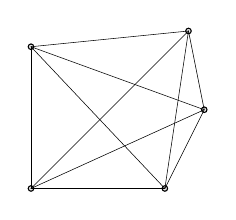
\begin{tikzpicture}
    \tkzDefPoint(0,0){v_1}
    \tkzDefPoint(1.7,0){v_2}
    \tkzDefPoint(2,2){v_3}
    \tkzDefPoint(0,1.8){v_4}
    \tkzDefPoint(2.2,1){v_5}
    \tkzDrawPoints(v_1,v_2, v_3, v_4, v_5)
    \tkzDrawSegments(v_1,v_2 v_2,v_3 v_3,v_4 v_4,v_5 v_1,v_5 v_1,v_3 v_3,v_5 v_2,v_4 v_1,v_4 v_2,v_5)
    \end{tikzpicture}\\
    klika $K_5$
\end{center}
\end{minipage}
\begin{minipage}{0.33\textwidth}
\begin{center}
    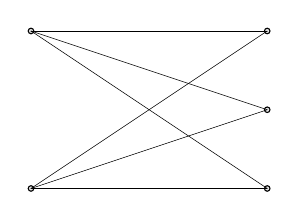
\begin{tikzpicture}
    \tkzDefPoint(0,2){v_1}
    \tkzDefPoint(0,0){v_2}

    \tkzDefPoint(3,0){v_3}
    \tkzDefPoint(3,1){v_4}
    \tkzDefPoint(3,2){v_5}
    \tkzDrawPoints(v_1, v_2, v_3, v_4, v_5)
    \tkzDrawSegments(v_1,v_4 v_1,v_5 v_2,v_4 v_2,v_5 v_1,v_3 v_2,v_3)
    \end{tikzpicture}\\
    graf dwudzielny $K_{2,3}$
\end{center}
\end{minipage}

\vspace{10px}

\begin{center}
    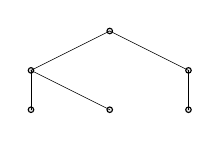
\begin{tikzpicture}
    \tkzDefPoint(1,1){v_1}

    \tkzDefPoint(0,0.5){v_2}
    \tkzDefPoint(2,0.5){v_3}

    \tkzDefPoint(0,0){v_4}
    \tkzDefPoint(1,0){v_5}
    \tkzDefPoint(2,0){v_6}
    \tkzDrawPoints(v_1, v_2, v_3, v_4, v_5, v_6)
    \tkzDrawSegments(v_1,v_2 v_1,v_3 v_2,v_4 v_2,v_5 v_3,v_6)
    \end{tikzpicture}\\
    drzewo
\end{center}

\vspace{10px}

\noindent
Grafy, które są spójne i nie zawierają żadnego cyklu nazywamy \textit{drzewami}. Mają one kilka równoważnych definicji, o czym mówi poniższe twierdzenie.

\vspace{5px}

\heading{Twierdzenie 1}

\noindent
Dany jest graf spójny $G$, który ma $n$ wierzchołków. Następujące warunki są sobie równoważnie
\begin{itemize}
    \item $G$ nie zawiera żadnego cyklu,
    \item w grafie jest dokładnie $n - 1$ krawędzi,
    \item pomiędzy dowolnymi dwoma wierzchołkami istnieje dokładnie jedna ścieżka, która nie przechodzi przez żaden wierzchołek więcej niż raz.
\end{itemize}

\heading{Dowód}

\noindent
Zauważmy, że dla $n = 1$ teza jest oczywista. Załóżmy, że $n \geqslant 2$. Najpierw wykażemy, że każdego z tych warunków wynika istnienie wierzchołka o stopniu $1$.

\vspace{10 px}
\noindent
Załóżmy nie wprost, że każdy wierzchołek ma stopień co najmniej $2$. Wówczas można łatwo obliczyć, że krawędzi jest co najmniej $\frac{2 \cdot n}{2} = n$, czyli pierwszy warunek nie może zajść.

\vspace{10 px}
\noindent
Wybierzmy pewien wierzchołek i rozpocznijmy w nim spacer po grafie. Z wierzchołka, w którym będziemy, wybierzemy krawędź, którą jeszcze nie szliśmy. Algorytm zakończymy, gdy trafimy w ten sposób do wierzchołka, w którym już byliśmy. Skoro stopień każdego grafu wynosi $2$, to nigdy nie utkniemy w żadnym z wierzchołków. Jeśli tak się stanie, to znaczy, że weszliśmy do tego wierzchołka co najmniej raz, a wtedy kończymy spacer. W taki sposób otrzymujemy cykl. Łatwo zauważyć, że z istnienia cyklu wynika istnienie dwóch ścieżek między dowolnymi jego dwoma wierzchołkami.

\vspace{10 px}
\noindent
Rozpatrzmy więc wierzchołek o stopniu $1$. Usuwając go wraz z krawędzią otrzymam graf o $n - 1$ wierzchołkach. W ten sposób nie zmieni się prawdziwość żadnego z warunków -- wierzchołek o stopniu $1$ nie może być częścią ani cyklu, ani dwóch ścieżek. Relacja liczby krawędzi do liczby cykli zostanie zachowana. Możemy więc skorzystać z zasady indukcji matematycznej i otrzymujemy tezę.

\vspace{10px}


\heading{Przykład 1}

\noindent
Dany jest prostokąt $m \times n$. Pokolorowano w nim $m + n$ pól. Wykazać, że da się wybrać pewne z pokolorowanych pól, tak, aby w każdej kolumnie i w każdym wierszu liczba wybranych pól była parzysta.

\vspace{5px}

\heading{Rozwiązanie}

\noindent
Rozpatrzmy graf, w którym wierzchołkami będą wiersze i kolumny. Jeśli pole zostało pokolorowane, to połączymy przyporządkowane mu wiersz i kolumnę. Otrzymany graf ma $m + n$ wierzchołków i $m + n$ krawędzi, czyli musi zawierać cykl. Wybierając przyporządkowane jego krawędziom pola otrzymujemy zbiór spełniający warunki zadania.
\qed

\vspace{10px}

\noindent
Ścieżkę, która przechodzi każdą z krawędzi dokładnie raz nazywamy \textit{ścieżką Eulera} na cześć szwajcarskiego matematyka Leonharda Eulera. Okazuje się, że stwierdzenie, czy w danym grafie istnieje ścieżka Eulera jest dość łatwe dzięki poniższemu twierdzeniu.

\vspace{10px}

\heading{Twierdzenie 2}

\noindent
Dany jest graf spójny o $n \geqslant 2$ wierzchołkach. Wówczas cykl Eulera istnieje, wtedy i tylko wtedy, gdy stopień każdego z wierzchołków jest liczbą parzystą.

\vspace{5px}

\heading{Dowód}

\noindent
Najpierw wykażemy, że cykl może istnieć tylko w takim wypadku. Przechodząc tą ścieżką, do każdego wierzchołka wejdziemy tyle samo razy, ile z niego wyjdziemy. Stąd więc każdy wierzchołek ma parzysty stopień, gdyż krawędzi ,,wejściowych'' i ,,wyjściowych'' jest tyle samo.

\vspace{10 px}

\noindent
Dowód, że gdy każdy ze stopni jest parzysty, to takowy cykl musi istnieć, jest nieco trudniejszy. Będziemy rozumować indukcyjnie po sumie liczby wierzchołków i krawędzi.

\vspace{5px}

\noindent
Zauważmy, że skoro graf jest spójny, to stopień żadnego z wierzchołków nie wynosi $0$ -- jest to co najmniej $2$. Rozumując podobnie jak w dowodzie Twierdzenia $1$ wykazujemy, że w rozpatrywanym grafie istnieje cykl -- nazwijmy go $\mathcal{C}$.

\vspace{5px}

\noindent
Usuńmy ten cykl z grafu. Nie musi pozostać spójny -- podzieli się on na pewne spójne składowe. Niemniej jednak każda ze składowych zawiera pewien wierzchołek $\mathcal{C}$. Na mocy założenia indukcyjnego w każdej z nich istnieje cykl Eulera. 

\vspace{5px}

\noindent
Możemy połączyć te cykle w jeden duży cykl. Wykażemy, że dwa rozłączne krawędziowo cykle o wspólnym wierzchołku możemy połączyć w jeden większy cykl. Korzystając z tego faktu posklejamy cykle po kolei ze sobą.

\vspace{5px}

\noindent
Załóżmy, że wspólnym wierzchołkiem cykli $\mathcal{A}$ i $\mathcal{B}$ jest pewien wierzchołek $c$. Wówczas startując z wierzchołka $c$, najpierw przechodzimy cykl $\mathcal{A}$. Wrócimy wtedy do wierzchołka~$c$. Wówczas przejdziemy cykl $\mathcal{B}$. W taki sposób otrzymamy jeden cykl.

\vspace{5px}

\noindent
Poniżej przestawiono rysunki poglądowe. Aby były czytelne, cykle przechodzą przez każdy wierzchołek dokładnie raz. Niemniej jednak w dowodzie takiego założenia nie poczyniliśmy.

\begin{minipage}{0.5\textwidth}
\begin{center}
    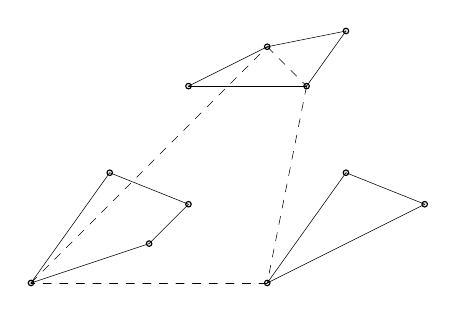
\begin{tikzpicture}
    \tkzDefPoint(0,0){a_1}
    \tkzDefPoint(1,1.4){a_2}
    \tkzDefPoint(2,1){a_3}
    \tkzDefPoint(1.5,0.5){a_4}
    \tkzDrawPoints(a_1,a_2,a_3,a_4)
    \tkzDrawSegments(a_1,a_2 a_2,a_3  a_3,a_4 a_4,a_1)
    
    \tkzDefPoint(2,2.5){b_1}
    \tkzDefPoint(3,3){b_2}
    \tkzDefPoint(4,3.2){b_3}
    \tkzDefPoint(3.5,2.5){b_4}
    \tkzDrawPoints(b_1,b_2,b_3,b_4)
    \tkzDrawSegments(b_1,b_2 b_2,b_3  b_3,b_4 b_4,b_1)
    
    \tkzDefPoint(3,0){c_1}
    \tkzDefPoint(4,1.4){c_2}
    \tkzDefPoint(5,1){c_3}
    \tkzDrawPoints(c_1,c_2,c_3)
    \tkzDrawSegments(c_1,c_2 c_2,c_3 c_3,c_1)

    \tkzDrawSegments[dashed](a_1,b_2 b_2,b_4 b_4,c_1 c_1,a_1)
    \end{tikzpicture}\\
    
\end{center}
\end{minipage}
\begin{minipage}{0.5\textwidth}
\begin{center}
    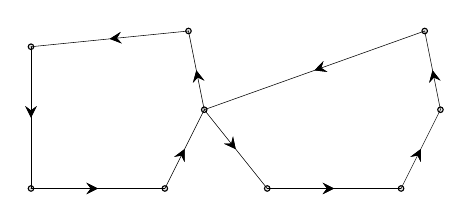
\begin{tikzpicture}
    \tkzDefPoint(0,0){v_1}
    \tkzDefPoint(1.7,0){v_2}
    \tkzDefPoint(2.2,1){v_3}
    \tkzDefPoint(2,2){v_4}
    \tkzDefPoint(0,1.8){v_5}
    \tkzDrawPoints(v_1,v_2, v_3, v_4, v_5)
    \tkzDrawSegments[arrowMe=stealth](v_1,v_2 v_2,v_3 v_3,v_4 v_4,v_5 v_5,v_1)


    \tkzDefPoint(3,0){a_1}
    \tkzDefPoint(4.7,0){a_2}
    \tkzDefPoint(5.2,1){a_3}
    \tkzDefPoint(5,2){a_4}
    \tkzDrawPoints(a_1,a_2, a_3, a_4)
    \tkzDrawSegments[arrowMe=stealth](a_1,a_2 a_2,a_3 a_3,a_4 a_4,v_3 v_3,a_1)
    \end{tikzpicture}\\
\end{center}
\end{minipage}

\vspace{5px}
\begin{problem}{1}
	W pewnym grafie każdy wierzchołek ma stopień co najmniej $100$. Wykazać, że w tym grafie istnieje ścieżka o długości co najmniej $101$.
\end{problem}

\begin{problem}{2}
	W pewnym kraju jest $n$ miast, przy czym każde dwa są połączone drogą albo torami kolejowymi. Pewien turysta planuje wyruszyć z pewnego miasta, odwiedzić każde miasto dokładnie raz, a następnie powrócić do wyjściowego miasta. Wykazać, że może tak wybrać wyjściowe miasto i tak zaplanować swoją trasę, aby zmienić środek transportu co najwyżej raz.
\end{problem}

%Source: Tournament of the towns 1986
\begin{problem}{3}
	W pewnym turnieju bierze udział $40$ drużyn. Pierwszego dnia każda z drużyn rozegrała jeden mecz. Drugiego dnia również. Wykazać, że istnieje pewne $20$ drużyn, takich, że każde dwie spośród nich jeszcze nie grały ze sobą meczu.
\end{problem}

%Source: Tournament of the towns 1986
\begin{problem}{4}
	W pewnym turnieju bierze udział $40$ drużyn. Pierwszego dnia każda z drużyn rozegrała jeden mecz. Drugiego dnia również. Wykazać, że istnieje pewne $20$ drużyn, takich, że każde dwie spośród nich jeszcze nie grały ze sobą meczu.
\end{problem}


\begin{problem}{5}
	W pewnym grafie o $n$ wierzchołkach ich stopnie wynoszą odpowiednio $d_1$, $d_2$, ..., $d_n$. Udowodnić, że istnieje taki podzbiór co najmniej $\sum^{n}_{i = 1} \frac{1}{1 + d_i}$ jego wierzchołków, że żadne dwa z nich nie są połączone krawędzią.
\end{problem}

%Source: https://artofproblemsolving.com/community/c6h455746p2560781
\begin{problem}{6}
	Hydra składa się z pewnej liczby głów, z której niektóre są połączone szyjami. Herkulers może odciąć wszystkie szyje wychodzące z pewnej głowy, jednak wówczas z tamtej głowy wyrastają szyję, którą łączą ją z głowami, z którymi nie była ona wcześnie połączona. Hydra jest pokonana, gdy rozpada się na dwie rozłączne części. Wyznaczyć najmniejsze $N$, że Herkules jest w stanie pokonać dowolną hydrę składającą się ze $100$ szyi.
\end{problem}


\newpage
% Rozdział 9 – Indukcja matematyczna 2

\theory{Indukcja matematyczna 2}

% dopisać, że indukcji trzeba zawsze próbować

\noindent
Indukcja, o której pisaliśmy wcześniej, korzystała z faktu, że jeśli teza zachodzi dla pewnej liczby $k$, to zachodzi również dla liczby $k + 1$. W nastepującym przykładzie pokażemy nieco ogólniejszą metodę, zwaną indukcją zupełną.

\vspace{10px}

\heading{Przykład 1}

\noindent
Niech $F_0 = 0$, $F_1 = 1$, $F_{n + 1} = F_n + F_{n - 1}$ dla $n \geqslant 1$ będą kolejnymi liczbami Fibonacciego. Wykazać, że każda dodatnia liczba całkowita może być przedstawiona w postaci sumy parami różnych liczb Fibonacciego.

\vspace{10px}

\heading{Rozwiązanie}


\vspace{10px}

% https://docs.google.com/viewer?a=v&pid=sites&srcid=ZGVmYXVsdGRvbWFpbnxpbW9jYW5hZGF8Z3g6NDA2NGM2NjkwZTJiYTg2Ng
% Wspomnieć o umocnieniu
\heading{Przykład 2}

\noindent
Wykaż, że
\[
	\frac{1}{2} \cdot \frac{3}{4} \cdot ... \cdot \frac{2n - 1}{2n} < \frac{1}{\sqrt{3n}}.
\]
%Source:
\begin{problem}{1}

\end{problem}


\newpage
% Rozdział 10 – Reszty kwadratowe

\theory{Podzielności}

% wprowadzenie symbolu v_p

\heading{Wykładniki peadyczne}

\heading{Własności $v_p$}

% Source: XIII OMJ, finals

\heading{Przykład 1}

Niech $a$, $b$ będą nieparzystymi liczbami całkowitymi, dla których $a^bb^a$ jest kwadratem liczby całkowitej. Wykazać, że liczba $ab$ również jest kwadratem liczby całkowitej.

\heading{Rozwiązanie}


%Source: https://om.mimuw.edu.pl/static/app_main/problems/om66_1r.pdf P1
\heading{Przykład 2}

Dane są takie niezerowe liczby całkowite, że liczba
\[
	\frac{a}{b} + \frac{b}{c} + \frac{c}{a}
\]
jest całkowita. Wykazać, że iloczyn $abc$ jest sześcianem liczby całkowitej.

\heading{Rozwiązanie}

% Source: https://s3.amazonaws.com/aops-cdn.artofproblemsolving.com/resources/articles/olympiad-number-theory.pdf Ex 3.3.1

\heading{Przykład 3}

Wykazać, że dla żadnej dodatniej liczby całkowitej $n$ większej od $1$ liczba
\[
	1 + \frac{1}{2} + \frac{1}{3} + ... + \frac{1}{n}
\]
nie jest liczbą całkowitą.

\heading{Rozwiązanie}

\heading{Wzór Legendre'a}

\heading{Przykład 4}

Udowodnić, że dla wszystkich liczb całkowitych $n$ liczba 
\[
	\frac{1}{n+1}{{2n}\choose{n}}
\]
jest całkowita.

\heading{Rozwiązanie}
% wzór Langrange'a z silniami


%Source:
\begin{problem}{1}

\end{problem}


\newpage
% Rozdział 11 – gry

\theory{Gry}

% coś o tym, czym jest gra i strategia wygrywająca

\heading{Przykład 1}

Ania i Bartek grają w następującą grę. Mają do dyspozycji stół w kształcie koła oraz dowolnie wiele monet o jednakowej średnicy, mniejszej od średnicy stołu. W każdym ruchu gracz kładzie monetę na stole tak, aby nie przykrywała żadnej innej monety. Gdy wykonanie ruchu nie jest możliwe, gracz którego jest kolej przegrywa. Rozstrzygnąc który z graczy ma startegię wygrywającą.

\heading{Rozwiązanie}

% komentarz – warto poszukać symetrii, zrobić małe przypadki



% analiza stanów – przykład gry z kamieniami
\heading{Przykład 2}

Na stole leży $10000$ kamieni. Ruch polega na zabraniu ze stołu $2$ lub $5$ kamieni. Dwaj gracze wykonują ruch na przemian, gdy gracz nie może wykonać ruchu przegrywa. Rozstrzygnąć, który z graczy – pierwszy czy drugi – ma strategię wygrywającą.

\heading{Rozwiązanie}

% tabelka ze stanami

% komentarz, że to podejście jest bardziej ogólne


\begin{problem}{1}
	Na tablicy napisano liczbę całkowitą dodatnią. W każdym ruchu zmazujemy napisaną liczbę $n$ na tablicy i piszemy nową liczbę. Jeśli $n$ była parzysta to piszemy na tablicy liczbę $\frac{1}{2}n$. Jeśli zaś liczba $n$ była nieparzysta, to zapisujemy jedną z liczb $3n - 1$ lub $3n + 1$. Czy -- niezależnie od tego, jaką liczbę zapisano na początku -- możemy, po skończenie wielu krokach, uzyskać na tablicy jedynkę?
\end{problem}


\begin{problem}{2}
	W lewym dolnym rogu planszy $m \times n$ stoi pionek. W każdym ruchu może zostać on przesunięty o dowolną liczbę pól w górę lub o dowolną liczbę pól w prawo. Wygrywa gracz, który postawi figurę w prawym górnym rogu. Rozstrzygnąć dla jakich wartości $(m, n)$ pierwszy gracz ma strategię wygrywającą.
\end{problem}

\begin{problem}{3}
	Na tablicy zapisano liczbę $10000000$. W każdym ruchu, o ile przed nim była zapisana liczba $n$, gracz zastępuje ją liczbą $n - 1$ lub $\left\lfloor\frac{n + 1}{2}\right\rfloor$. Gracz, który zapisze liczbę $1$ wygrywa. Który z graczy – pierwszy czy drugi – ma strategię wygrywającą?
\end{problem}

\begin{problem}{4}
	Dwaj gracze na przemian stawiają kółko i krzyżyk w polach nieskończonej planszy. Gracz wygrywa, gdy istnieje kwadrat $2\times2$ ułożony z jego symboli. Wykazać, że drugi gracz może grać tak, aby pierwszy gracz nie był w stanie wygrać.
\end{problem}

\begin{problem}{5}
	Nauczyciel wraz z 30 uczniami gra w grę na nieskończonej kartce w kratkę. Zaczyna on, po czym ruch wykonuje każdy z 30 uczniów, po czym znów nauczyciel, po czym uczniowie i tak dalej. W każdym ruchu należy pokolorować jeden z boków kratki, który nie został wcześniej pokolorowany. Nauczyciel wygrywa, gdy na planszy znajduje się prostokąt $2 \times 1$ lub $1 \times 2$, że wszystkie jego boki są pokolorowane, ale odcinek wewnątrz niego nie jest. Udowodnij, że ma on strategię wygrywającą.
\end{problem}

\begin{problem}{6}
	$20$ dziewczyn usiadło w kółku. Na początku jedna z nich trzyma $N < 19$ kamieni. W każdym ruchu jedna z dziewczyn, która posiada co najmniej dwa kamienie daje po jednym każdej ze swoich sąsiadek. Gra kończy się, gdy każda z dziewczyn trzyma co najwyżej jeden kamień. Wykazać, że gra musi się skończyć po skończonej liczbie ruchów.
\end{problem}

\newpage
% Rozdział 12 – bardziej zaawansowanie nierówności

\theory{Bardziej zaawansowane nierówności}

\noindent
Na początku udowodnimy dwie bardzo znane nierówności. 

\vspace{10px}

% nierówność Cauchego–Schwarza
\heading{Nierówność Cauchego–Schwarza}

\noindent
Dla liczb rzeczywistych $a_1, a_2, ..., a_n$ oraz $b_1, b_2, ..., b_n$ zachodzi nierówność
\[
	\left(a_1^2 + a_2^2 + ... + a_n^2\right)\left(b_1^2 + b_2^2 + ... + b_n^2\right) \geqslant \left(a_1b_1 + a_2b_2 + ... + a_nb_n\right).
\]

\heading{Dowód}

\noindent
Przyjmijmy, że funkcja $f$ jest dana wzorem
\[
	f(x) = \sum^{n}_{i=1} (a_ix - b_i)^2 = \left(\sum^{n}_{i=1} a_i^2\right) x^2 - 2\left(\sum^{n}_{i=1} a_ib_i\right) x + \sum^{n}_{i=1} b_i^2.
\]
Zauważmy, że jest to suma funkcji przyjmujących wartości nieujemne, a więc sama przyjmuje tylko wartości nieujemne. Stąd też jej wyróżnik $\Delta$ będzie niedodatni
\[
	\Delta = 4\left(\sum^{n}_{i=1} a_ib_i\right)^2 - 4  \left(\sum^{n}_{i=1} a_i^2\right)  \left(\sum^{n}_{i=1} b_i^2\right) \leqslant 0,
\]
co jest równoważnie tezie.

\qed

\vspace{10px}

% ta sama w formie Engela

\heading{Nierówność Cauchego–Schwarza w formie Engela}

\noindent
Dla liczb dodatnich $a_1, a_2, ..., a_n$ oraz $b_1, b_2, ..., b_n$ zachodzi nierówność
\[
	\frac{a_1}{b_1} + \frac{a_2}{b_2} + ... + \frac{a_n}{b_n} \geqslant \frac{\left(a_1 + a_2 + ... + a_n\right)^2}{a_1b_1 + a_2b_2 + ... + a_nb_n}.
\]

\heading{Dowód}

\noindent
Zauważmy, że na mocy nierówności Cauchego-Schwarza prawdą jest, że
\begin{gather*}
	\left(\sum^{n}_{i = 1} \left(\sqrt{\frac{a_i}{b_i}}\right)^2 \right) \left(\sum^{n}_{i = 1} \left(\sqrt{a_ib_i}\right)^2 \right) \geqslant \left(\sum^{n}_{i = 1} \sqrt{a_ib_i} \cdot \sqrt{\frac{a_i}{b_i}} \right).
\end{gather*}
Jest to równoważnie nierówności
\[
	\left(\sum^{n}_{i = 1} \frac{a_i}{b_i} \right) \left(\sum^{n}_{i = 1} a_ib_i \right) \geqslant \left(\sum^{n}_{i = 1} a_i^2 \right),
\]
z której w oczywisty sposób wynika teza.

\qed
\newpage

\noindent

% ciągi jednomonotoniczne

\noindent
Przejdziemy teraz do nierówności między ciągami jednomonotonicznymi. Ma ona bardzo ciekawy dowód, do którego będzie potrzebny nam następujący lemat.

\vspace{10px}

\heading{Lemat 1}

\noindent
Dane są liczby rzeczywiste $a_1 \geqslant a_2$ oraz $b_1 \geqslant b_2$. Wówczas zachodzi nierówność
\[
	a_1b_1 + a_2b_2 \geqslant a_1b_2 + a_2b_1.
\] 
Jeśli zaś $a_1 \geqslant a_2$ oraz $b_1 \leqslant b_2$, to zachodzi
\[
	a_1b_1 + a_2b_2 \leqslant a_1b_2 + a_2b_1.
\] 

\heading{Dowód}

\noindent
Zauważmy, że
\[
	a_1b_1 + a_2b_2 \geqslant a_1b_2 + a_2b_1 \iff (a_1 - a_2)(b_1 - b_2) \geqslant 0,
\]
\[
	a_1b_1 + a_2b_2 \leqslant a_1b_2 + a_2b_1 \iff (a_1 - a_2)(b_1 - b_2) \leqslant 0,
\]
Teza lematu wynika wprost z założeń.

\qed

\vspace{10px}

% tutaj opis przekształceń, sortowania bąbelkowego
% ,,z tego algorytmu wynika następujące twierdzenie

\heading{Twierdzenie o ciągach jednomonotonicznych}

\noindent
Liczby $a_1 \geqslant a_2 \geqslant ... \geqslant a_n$ oraz $b_1 \geqslant b_2 \geqslant ... \geqslant b_n$ są rzeczywiste. Niech $b_1', b_2', ..., b_n'$ będzie permutacją liczb $b_1, b_2, ..., b_n$. Wówczas zachodzą nierówności
\[
	a_1b_1 + a_2b_2 + ... + a_nb_n \geqslant a_1b_1' + a_2b_2' + ... + a_nb_n' \geqslant a_1b_n + a_2b_{n - 1} + ... + a_nb_1.
\]

\heading{Dowód}

\noindent
Rozpatrzmy pewną permutację $b_1', b_2', ..., b_n'$ liczb $b_1, b_2, ..., b_n$.  Zamieńmy liczby $b'_i$ oraz~$b'_{i + 1}$ miejscami i zobaczmy co stanie się z wartością wyrażenia, nazwijmy go $W$:
\[
	a_1b_1' + a_2b_2' + ... + a_nb_n'.
\]
Składnik $a_ib_i'$ zostanie zastąpiony przez $a_ib_{i + 1}'$, zaś $a_{i + 1}b_{i + 1}'$ zostanie zastąpiony przez $a_{i + 1}b_i'$. Inne składniki pozostaną bez zmian. Skoro $a_i \geqslant a_{i + 1}$, to z Lematu~1 wynika, że
\[
	a_ib_{i + 1}' + a_{i + 1}b_i' \leqslant a_ib_i' + a_{i + 1}b_{i + 1}', \quad \text{gdy} \; b_i \geqslant b_{i + 1},
\]
\[
	a_ib_{i + 1}' + a_{i + 1}b_i' \geqslant a_ib_i' + a_{i + 1}b_{i + 1}', \quad \text{gdy} \; b_i \leqslant b_{i + 1}.
\]

\vspace{10px}

\noindent
Jeśli więc liczby $b'_i$ oraz $b'_{i + 1}$ są posortowane odwrotnie do ciągu $\{a_i\}$, to zmieniając ich kolejności możemy zwiększyć wartość wyrażenia $W$.
Wykonując wiele takich zamian, za każdym razem wartość $W$ wzrośnie. Również liczba par postaci $(b_i', b_j')$, gdzie $i > j$ oraz $b_i' < b_j'$ maleje o $1$ przy każdym przestawieniu. Stąd w pewnym momencie otrzymamy permutację, w którym nie możemy wykonać rozpatrywanej operacji. Znaczy to tyle, że $b'_i \geqslant b'_{i + 1}$ dla wszystkich możliwych wartości liczby $i$, czyli po prostu $b'_i = b_i$. Finalnie, wartość rozpatrywanego wyrażenia $W$ jest równa
\[
	a_1b_1 + a_2b_2 + ... + a_nb_n.
\]
Skoro przy każdym ruchu wartość tego wyrażenia rosła, to jego finalna wartość jest większa od wartości początkowej.

\vspace{10px}

\noindent
Dowodzi to jednej z dwóch postulowanych nierówności. Dowód drugiej z nich jest analogiczny, tylko zamieniamy miejscami $b_i'$ posortowane jednakowo jak ciąg $\{a_i\}$.

\qed

\vspace{10px}

\noindent
Przyjmijmy, że ciągi $(a_1, a_2, ..., a_n)$ oraz $(b_1, b_2, ..., b_n)$ są \textit{jednakowo monotoniczne}, gdy dla dowolnych indeksów $i$ oraz $j$ zachodzi
\[
	a_i > a_j \quad \iff \quad b_i > b_j,
\]
zaś \textit{odwrotnie monotoniczne}, gdy
\[
	a_i > a_j \quad \iff \quad b_i < b_j.
\]

\vspace{10px}

\noindent
Przykładowo ciągi $(2, 1, 3)$ oraz $(101, 100, 102)$ są jednakowo monotoniczne, zaś ciągi $(1, 2, 3)$ oraz $(10, 9, 8)$ są odwrotnie monotoniczne. Możemy teraz inaczej sformułować wykazaną wcześniej nierówność.

\vspace{10px}

\noindent
Jeśli mamy dwa ciągi $(a_1, a_2, ..., a_n)$ oraz $(b_1, b_2, ..., b_n)$ i rozpatrzymy wszystkie ich możliwe permutacje, to wartość wyrażenia
\[
	a_1b_1 + a_2b_2 + ... a_nb_n
\]
będzie największa, gdy ciągi $\{a_i\}$ oraz $\{b_i\}$ są jednakowo monotoniczne, zaś najmniejsza, gdy $\{a_i\}$ oraz $\{b_i\}$ są odwrotnie monotoniczne.

\vspace{10px}

\heading{Przykład 2}

\noindent
Liczby $a_1$, $a_2$, ..., $a_n$ są dodatnie. Wykazać, że zachodzi nierówność
\[
	a_1^3 + a_2^3 + ... + a_n^3 \geqslant a_1^2a_2 + a_2^2a_3 + ... + a^2_{n - 1}a_n + a_n^2a_1.
\]

\heading{Rozwiązanie}

\noindent
Rozpatrzmy ciągi:
\[
	(a_1^2, a_2^2, ..., a_n^2) \quad \text{oraz} \quad (a_1, a_2, ..., a_n).
\]
Zauważmy, że są one jednakowo monotoniczne, gdyż
\[
	a_i^2 > a_j^2 \iff a_i > a_j.
\]
Na mocy nierówności o ciągach jednomonotonicznych prawdą jest, że
\[
	a_1^2 \cdot a_1 + a_2^2 \cdot a_2 + ... + a_n^2 \cdot a_n \geqslant a_1^2 \cdot a_2 + a_2^2 \cdot a_3 + ... + a_n^2 \cdot a_1,
\]
co jest równoważne tezie.

\newpage

\heading{Cykliczność a symetryczność}

\noindent
Bardzo często przy rozwiązywaniu nierówności zdarzają się stwierdzenia typu ,,bez straty ogólności załóżmy, że''. Zazwyczaj chodzi o to, że rozpatrywany jest jeden przypadek, a inne są do niego analogiczne. Nie zawsze jednak są one analogiczne. Chociażby w Przykładzie 2 nie można założyć bez straty ogólności, że
\[
	a_1 \geqslant a_2  \geqslant ... \geqslant a_n,
\]
gdyż przypadek, gdy $n = 4$ i $a_1 \geqslant a_3 \geqslant a_2 \geqslant a_4$ nie daje się łatwo sprowadzić do przypadku powyższego.
\vspace{10px}

\noindent
Zdefiniujmy wyrażenie algebraiczne jako \textit{symetryczne}, gdy wyrażenie dla liczb $(a_1, a_2, ..., a_n)$ nie zmieni się, gdy rozpatrzymy dowolną ich permutację. Chociażby wyrażenie
\[
	abc + a + b + c
\]
jest symetryczne. Chociażby rozpatrując permutację $(b, a, c)$ krotki $(a, b, c)$ otrzymamy
\[
	bac + b + a + c = abc + a + b + c.
\]

\noindent
Wyrażenie algebraiczne nazwiemy \textit{cyklicznym}, gdy wyrażenie dla liczb $(a_1, a_2, ..., a_n)$ nie zmieni się, gdy rozpatrzymy dowolne ich przestawienie cykliczne -- $(a_k, a_{k + 1}, ..., a_n, a_1,  a_{k - 1})$. Wyrażenie
\[
	ab^2 + bc^2 + ca^2
\]
jest cykliczne. Dla przykładu rozpatrując przestawienie cykliczne $(c, a, b)$ krotki $(a, b, c)$ otrzymamy
\[
	ca^2 + ab^2 + bc^2 = ab^2 + bc^2 + ca^2.
\]
Nie jest ono symetryczne, gdyż dla permutacji $(b, a, c)$ krotki $(a, b, c)$ mamy
\[
	ba^2 + ac^2 + cb^2 \neq ab^2 + bc^2 + ca^2
\]

\noindent
Nierówność nazwiemy symetryczną albo cykliczną, gdy rozpatrując odpowiednio permutację lub przestawienie cykliczne zmiennych, w oczywisty sposób otrzymana nierówność jest równoważna nierówności wyjściowej.
\begin{itemize}
	\item Gdy nierówność jest symetryczna, to można założyć ustalony porządek liczb. 
	\item Jeśli zaś nierówność jest jedynie cykliczna, to można chociażby założyć, że pewna zmienna jest największa lub najmniejsza spośród wszystkich. Nie można jednak ustalać sobie ich porządku!
\end{itemize}



%Source: Wędrówki po krainie nierówności 3.5 przykład 2
\begin{problem}{1}
	Dane są liczby dodatnie $a$, $b$, $c$. Wykaż, że zachodzi nierównośc
	\[
		\frac{a}{2b + c} + \frac{b}{2c + a} + \frac{c}{2a + b} \geqslant 1. 
	\]
\end{problem}

%Source: Wędrówki po krainie nierówności 3.5 przykład 3
\begin{problem}{2}
	Udowodnić, że dla dowolnych liczb dodatnich $a$, $b$, $c$ zachodzi nierówność
	\[
		a^3b + b^3c + c^3a \geqslant a^2bc + ab^2c + abc^2.
	\]
\end{problem}

%Source: Wędrówki po krainie nierówności 3.5.3
\begin{problem}{3}
	Udowodnić, że dla dowolnych liczb rzeczywistych $\alpha_1, \; \alpha_2, \; \alpha_n$, gdzie $n \geqslant 2$ zachodzi nierówność
	\[
		\sin{\alpha_1}\cdot ... \cdot \sin{\alpha_n} + \cos{\alpha_1}\cdot ... \cdot \cos{\alpha_n} \leqslant 1.
	\]
\end{problem}

%Source: well-known
\begin{problem}{4}
	Dane są liczby rzeczywiste $a_1 \geqslant a_2 \geqslant ... \geqslant a_n$ oraz $b_1 \geqslant b_2 \geqslant ... \geqslant b_n$. Wykazać, że zachodzi nierówność
	\[
		n(a_1b_1 + a_2b_2 + ... + a_nb_n) \geqslant (a_1 + a_2 + ... + a_n)(b_1 + b_2 + ... + b_n).
	\]
\end{problem}

%Source: https://omj.edu.pl/uploads/attachments/omj2017-tresci.pdf
% Obóz OMJ 2017 poziom OMJ P 21
\begin{problem}{5}
	Rozstrzygnąć, czy dla dowolnych liczb dodatnich $a$, $b$, $c$ zachodzi nierównośc
	\[
		a^2b^3 + b^2c^3 + c^2a^3 \leqslant ab^4 + bc^4 + ca^4.
	\]
\end{problem}


\newpage
% Rozdział 13 – Równania funkcyjne i wielomianowe

\theory{Równania funkcyjne 2}

\noindent
W niniejszym rozdziale poszerzymy naszą wiedzę na temat równań funkcyjnych. Nie będą to już jedynie sztampowe zadania na podstawienia i wykazywanie różnowartościowości/surjektywności funkcji. Na początku zastanówmy się nad funkcjami, które spełniają równanie
\[
	f(x) + f(y) = f(x + y).
\]
Powyższa zależność jest zwana \textit{równaniem Cauchego}.

\vspace{10px}

\heading{Przykład 1}

\noindent
Wyznaczyć wszystkie funkcje $f:\mathbb{Q}\longrightarrow\mathbb{Q}$, które dla dowolnych $x, y \in \mathbb{Q}$ spełniają warunek
\[
	f(x) + f(y) = f(x + y).
\]

\heading{Rozwiązanie}

\noindent
Na początku zauważmy, że dla dowolnej dodatniej liczby całkowitej zachodzą równości
\begin{align*}
	f(nx) &= f((n - 1)x) + f(x) = f((n - 2)x) + f(x) + f(x) = ... = \\
	&=  \underbrace{f(x) + ... + f(x)}_{n} = nf(x).
\end{align*}
Wykonując podstawienie $x = y = 0$ otrzymujemy, że
\begin{align*}
	f(0) + f(0) &= f(0), \\
	f(0) &= 0.
\end{align*}
Postawmy $y = -x$. Wówczas
\begin{align*}
	f(x) + f(-x) &= f(0) = 0, \\
	f(-x) &= -f(x).
\end{align*}
Łącząc powyższą równość z pierwszą z otrzymanych zależności otrzymujemy, że
\[
	f(-nx) = -f(nx) = nf(x).
\]
Możemy więc wywnioskować, że $f(nx) 
= nf(x)$ dla dowolnej liczby całkowitej $n$ oraz dowolnej liczby rzeczywistej $x$. Wstawiając $x = \frac{p}{q}$ oraz $n = q$ otrzymamy
\[
	qf\left(\frac{p}{q}\right) = f(p).
\]
Zaś dla $x = 1$ i $n = p$ mamy
\[
	f(p) = pf(1).
\]
Stąd
\begin{align*}
	qf\left(\frac{p}{q}\right) &= pf(1), \\
	f\left(\frac{p}{q}\right) &= \frac{p}{q} \cdot f(1).
\end{align*}
Skoro $f(1)$ jest stałe, to funkcja $f$ jest funkcją postaci $f(x) = ax$ dla pewnej liczby wymiernej $a$. Łatwo sprawdzić, że takie funkcje spełniają warunki zadania.

\qed

\noindent
Rozsądną więc wydaje się hipoteza, że jeśli funkcja $f$ jest zdefiniowana na liczbach rzeczywistych i przyjmuje wartości rzeczywiste oraz spełnia równanie Cauchego, to musi być funkcją postaci $f(x) = ax$ dla pewnej liczby rzeczywistej $a$. Nie jest to jednak prawda! Taka implikacja nie zachodzi.

\vspace{10px}

\noindent
Jaka więc jest funkcja rzeczywista, która spełnia równanie Cauchego, a nie jest funkcją liniową? Skonstruowanie takiej funkcji jest możliwe, gdy założymy \textit{pewnik wyboru}. To ten sam aksjomat, z którego założenia wynika  paradoks Banacha-Tarskiego. Nie będziemy tutaj zgłębiać tego tematu, ważny jest fakt, że z samego równania Cauchego dla funkcji rzeczywistych nie wynika ich liniowość.

\vspace{10px}

\noindent
Jaka więc jest funkcja rzeczywista, która spełnia równanie Cauchego, a nie jest funkcją liniową? Skonstruowanie takiej funkcji jest możliwe, gdy założymy \textit{pewnik wyboru}. To ten sam aksjomat, z którego założenia wynika  paradoks Banacha-Tarskiego. Nie będziemy tutaj zgłębiać tego tematu, ważny jest fakt, że z samego równania Cauchego dla funkcji rzeczywistych nie wynika ich liniowość.

\vspace{10px}

\noindent
Można jednak dołożyć pewne założenie do równania Cauchego, aby uzyskać liniowość rozpatrywanej funkcji. Mówi o tym następujące twierdzenie.

\vspace{10px}

\heading{Twierdzenie 1}

\noindent
Jeśli pewna funkcja $f:\mathbb{R}\longrightarrow\mathbb{R}$ dla dowolnych liczb rzeczywistych $x, y$ spełnia warunek

\[
	f(x) + f(y) = f(x + y).
\]
oraz jest funkcja niemalejącą, to wówczas $f(x) = ax$.

\vspace{10px}

\heading{Dowód}

\noindent
Przyjmijmy $a = f(1)$. Na mocy Przykładu 1 mamy, że 
\[
	f(q) = aq \quad \text{ dla dowolnej liczby wymiernej } q.
\]
Załóżmy nie wprost, że dla pewnej liczby rzeczywistej $t$ zachodzi równość
\[
	f(t) = a(t + t_0), \; t_0 \neq 0.
\]
Przyjmijmy, że $t_0 > 0$. Drugi przypadek będzie analogiczny.
Znanym faktem jest, że w przedziale $(t, \; t + t_0)$ jest pewna liczba wymierna $q_0$. Mamy wówczas
\[
	f(q_0) = aq_0 < a(t + t_0) = f(t).
\]
Wiedząc, że $q_0 > t$ otrzymujemy sprzeczność z tym, że $f$ jest niemalejąca.

\qed

\newpage
\noindent
Analogiczne twierdzenia można udowodnić, gdy fakt, że $f$ jest malejąca, zastąpić tym, że 
\begin{itemize}
	\item $f(x) > 0$, dla dowolnego $x > 0$,
	\item $f(x) < 0$, dla dowolnego $x < 0$,
	\item $f$ jest ograniczona na przedziale -- $f(x) < M$, dla dowolnego $a < x < b$, dla pewnych liczb rzeczywistych $a < b$ oraz $M$,
	\item $f$ jest ciągła.
\end{itemize}
Warto zaznaczyć, że różnowartościowość funkcji $f$ nie wystarcza, aby była ona liniowa. 


\vspace{10px}

\heading{Przykład 2}
% https://artofproblemsolving.com/community/q1h1871345p12695350

\noindent
Znajdź wszystkie funkcje $f$ ze zbioru liczb rzeczywistych w zbiór liczb rzeczywistych, że dla dowolnych liczb rzeczywistych $x$, $y$ zachodzą równości
\[ 
	f(x) + f(y) = f(x + y) \quad \text{oraz} \quad f(x)f(y) = f(xy).
\]

\vspace{5px}

\heading{Rozwiązanie}

\noindent
Wstawiając do drugiego równania $x = y$ otrzymujemy
\[
	f(x^2) = f(x)f(x) = f(x)^2 \geqslant 0.
\]
Niech $t$ będzie liczbą nieujemną. Wstawiając $x = \sqrt{t}$ do powyższego równania otrzymujemy $f(t) \geqslant 0$. Czyli $f$ przyjmuje wartości nieujemne dla argumentów nieujemnych.

\vspace{10px}
\noindent
Wykażemy, że $f$ jest niemalejąca. W tym celu rozpatrzmy dwie liczby rzeczywiste $a > b$. Mamy
\[
	f(a) = f(a - b) + f(b) \geqslant f(b),
\]
co dowodzi postulowanej własności.

\vspace{10px}
\noindent
Na mocy Twierdzenia 1 mamy, że $f(x) = ax$ dla pewnej liczby rzeczywistej $a$. Podstawiając to do drugiego równania otrzymamy
\begin{align*}
	ax \cdot ay &= axy, \\
	a^2 &= a.
\end{align*}
Stąd $a = 0$ lub $a = 1$. Łatwo sprawdzić, że obie funkcje $f(x) = 0$ i $f(x) = x$ spełniają warunki zadania.

\qed

\vspace{10px}
\noindent 
Warto zwrócić uwagę na sposób, w jaki wykazano, że funkcja $f$ jest niemalejąca. Da się go spotkać w wielu zadaniach tego rodzaju. 

\vspace{10px}

% https://web.evanchen.cc/handouts/FuncEq-Intro/FuncEq-Intro.pdf Ex 2.1
\heading{Przykład 3}

\noindent
Znajdź wszystkie funkcje $ f:\mathbb{R}\to\mathbb{R} $ dla których 
\[
	f(f(x)^2 + f(y)) = xf(x) + y,
\]
dla dowolnych liczb rzeczywistych $x, y$.

\heading{Rozwiązanie}

\noindent
Zacznijmy od najprostszego podstawienia. Weźmy $x = y = 0$. Wówczas otrzymamy
\[
	f(f(0)^2 + f(0)) = 0.
\]
Oznacza to, że istnieje  liczba rzeczywista $a = f(0)^2 + f(0)$, że $f(a) = 0$. Wstawmy $x = a$
\begin{align*}
	f(f(a)^2 + f(y)) &= af(a) + y, \\
	f(f(y)) &= y.
\end{align*}
Następnie zastąpmy $x$ przez $f(x)$ w wyjściowym równaniu
\begin{align*}
	f(f(f(x))^2 + f(y)) &= f(x)f(f(x)) + y, \\
	f(x^2 + f(y)) &= xf(x) + y.
\end{align*}
W wyjściowym równaniu mieliśmy
\[
	f(f(x)^2 + f(y)) = xf(x) + y.
\]
Łącząc oba powyższe równania otrzymujemy
\[
	f(f(x)^2 + f(y)) = f(x^2 + f(y)).
\]
Wykażemy, że funkcja $f$ jest różnowartościowa. Zakładamy w tym celu, że dla pewnych liczb rzeczywistych $a$, $b$ zachodzi $f(a) = f(b)$. Wtedy
\[
	a = f(f(a)) = f(f(b)) = b.
\]
Stąd
\begin{align*}
	f(f(x)^2 + f(y)) &= f(x^2 + f(y)) \\
	f(x)^2 + f(y) &= x^2 + f(y) \\
	f(x)^2 &= x^2.
\end{align*}
Mamy więc, że dla każdej liczby rzeczywistej $x$ zachodzi $f(x) = x$ lub $f(x) = -x$. Załóżmy więc, że dla pewnych niezerowych liczb rzeczywistych zachodzi $f(a) = -a$ i $f(b) = b$. Biorąc $x = a$ i $y = b$ otrzymujemy
\[
	f(a^2 - b) = -a^2 + b.
\]
W zależności od tego, czy $f(a^2 - b)$ jest równe $a^2 - b$ czy $-a^2 + b$ otrzymujemy sprzeczność z niezerowością obu liczb $a$, $b$. Stąd albo $f(x) = x$ dla wszystkich liczb rzeczywistych $x$ albo $f(x) = -x$ dla wszystkich liczb rzeczywistych. Sprawdzając otrzymujemy, że obie te funkcje spełniają warunki zadania.

\qed

\vspace{10px}
\noindent
Należy zauważyć, że z faktu $f(x)^2 = x^2$ nie wynika jeszcze to, że $f(x) = x$ dla wszystkich $x$ lub $f(x) = -x$ dla wszystkich $x$. Może się bowiem zdarzyć na przykład, że $f(1) = 1$ i~$f(2) = -2$. Jest to dość znana pułapka i~warto zwrócić na nią uwagę.

%Source:
\begin{problem}{1}

\end{problem}


\newpage
% Rozdział 14 – twierdzenia z teorii liczb

\theory{Twierdzenia z teorii liczb}

% skrypt bardziej teoretyczny
% zadania nie zawsze są z nim związane, ale są pouczające

\noindent
Na potrzeby natstepującego lematu i twierdzenia, dla liczby całkowitej $n$ oraz parami względnie pierwszych liczb $m_1$, ..., $m_k$ przyjmiemy
\[
	G(n) = (n \;(\text{mod } m_1), n \;(\text{mod } m_2), ..., n \;(\text{mod } m_k)).
\]


% obserwacja, że G(n) może przyjmować m_1m_2...m_k wartości

\heading{Lemat 1}

\noindent
Dane są parami względnie pierwsze liczby $m_1$, ..., $m_k$ oraz dodatnie liczby całkowite~$x$,~$y$ spełniające $m_1m_2\cdot ... \cdot m_k > x > y > 0$. Wykazać, że wówczas
\[
	G(x) \neq G(y).
\]

\heading{Dowód}



\heading{Chińskie twierdzenie o resztach}

\noindent
Dane są parami względnie pierwsze liczby $m_1$, ..., $m_k$ oraz pewne liczby całkowite $a_1$, ..., $a_k$. Wówczas istnieje taka liczba całkowita $x$, że zachodzą przystawania
\begin{gather*}
	x \equiv a_1 \pmod{m_1}, \\
	x \equiv a_2 \pmod{m_2}, \\
	..., \\
	x \equiv a_k \pmod{m_k}.
\end{gather*}

\heading{Dowód}

% potem komentarz, że to znaczy tyle, że ,,jakie przystawania sobie zażyczymy, takie mamy

\heading{Symbol Legendre'a}

\noindent
Dla pewnej liczby pierwszej $p$ oraz liczby całkowitej $n$ przyjmiemy
\[
	\left(\frac{n}{p}\right) = 
	\begin{cases}
		\phantom{-}1 \text{, gdy istnieje taka liczba całkowita } a \not\equiv 0 \text{, że } n \equiv a^2 \pmod{p}\\
		-1\text{, gdy nie istnieje taka liczba całkowita } a \not\equiv 0 \text{, że } n \equiv a^2 \pmod{p} \\
		\phantom{-}0 \text{, gdy } n \equiv 0 \pmod{p}\\
	\end{cases}
\]

\noindent
W pierwszym przypadku powiemy, że $n$ jest \textit{resztą kwadratową}, a w drugim, że $n$ jest \textit{nieresztą kwadratową}.


\heading{Twierdzenie 2}

\noindent
Dana jest liczba pierwsza $p$ oraz liczby całkowite $a$, $b$. Wówczas zachodzi równość
\[
	\left(\frac{a}{p}\right)\left(\frac{b}{p}\right) = \left(\frac{ab}{p}\right).
\]

\heading{Dowód}

\heading{Pierwiastki pierwotne modulo $p$}

% bez dowodu!!!

\vspace{10px}


\vspace{10px}

\heading{Przykład 1}

\noindent
Wykazać, że dla dodatniej liczby całkowitej, która nie jest podzielna przez $p - 1$ zachodzi przystawanie
\[
	1^k + 2^k + 3^k + ... + p^k \equiv 0 \pmod{p}.
\]

\heading{Rozwiązanie}
%Source: Burek 11
\begin{problem}{1}
	Wykazać, że dodatnia liczba całkowita $n$ ma co najwyżej $2\sqrt{n}$ dzielników.
\end{problem}

%Source: Burek 11
\begin{problem}{2}
	Liczbę nazwiemy \textit{wielodzielną}, jeśli ma co najmniej $1000$ dzielników. Rozstrzygnąć, czy istnieje taka liczba całkowita $n$, że liczby
	\[
		n, n + 1, n + 2, ..., n + 1000
	\]
	są wielodzielne.
\end{problem}

%Source: Burek 11
\begin{problem}{3}
	Niech $d(n)$ oznacza liczbę dodatnich dzielników liczby $n$ -- włączając liczby $1$ i $n$. Wykazać, że istnieje nieskończenie wiele dodatnich liczb całkowitch $n$, dla których liczba $\frac{n}{d(n)}$ również jest całkowita.
\end{problem}

%Source: own
\begin{problem}{4}
	Dana jest nieparzysta liczba pierwsza $p$. Obliczyć wartość wyrażenia
	\[
		\left(\frac{0}{p}\right) + 
		\left(\frac{1}{p}\right) + 
		... +
		\left(\frac{p - 1}{p}\right).
	\]
\end{problem}

%Source: Burek 12
\begin{problem}{5}
	Niech $p$ będzie liczbą pierwszą dającą resztę $2$ z dzielenia przez $3$. Dla pewnych liczb całkowitych $a$, $b$ liczba $a^3 - b^3$ jest podzielna przez $p$. Wykazać, że liczba $a - b$ również jest podzielna przez $p$.
\end{problem}


%Source: Burek P201
\begin{problem}{6}
	Niech $a_1, ..., a_n$ oraz $b_1, ..., b_n$ będą dodatnimi liczbami całkowitymi, że dla każdej liczby całkowitej $n - 1\geqslant i \geqslant 0$ zachodzi nierówność $b_{i + 1} \geqslant 2b_{i}$. Wykazać, że istnieje nieskończenie wiele liczb całkowitych $k$, że nie zachodzi żadne z przystawań
	\begin{gather*}
		k \equiv a_1 \pmod{b_1}, \\
		k \equiv a_2 \pmod{b_2}, \\
		.., \\
		k \equiv a_n \pmod{b_n}.
	\end{gather*}
\end{problem}



\newpage
% Rozdział 15 - Grafy skierowane

\theory{Grafy skierowane}

\heading{Definicje}

\noindent
\textit{Grafem skierowanym} nazywamy taki graf, w którym każda z krawędzi jest skierowana jedną ze stron. Może zdarzyć się, że pomiędzy wierzchołkami są dwie krawędzie, każda skierowana w inną stronę. Przykład takiego grafu znajduje się na poniższym rysunku.

\begin{center}
	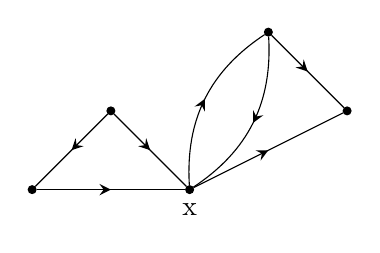
\begin{tikzpicture}
		\tikzset{vertex/.style = {shape=circle,draw, inner sep = 1pt, fill=black}}
		\tikzset{edge/.style = {arrowMe=stealth}}

		\node[vertex] (A) at (-2,2) {};
		\node[vertex] (B) at (-1,3) {};
		\node[vertex, label=below:x] (C) at (0,2) {};
		\node[vertex] (D) at (2,3) {};
		\node[vertex] (E) at (1,4) {};

		\draw[edge] (B) to (A);
		\draw[edge] (B) to (C);
		\draw[edge] (A) to (C);
		\draw[edge] (C) to (D);
		\draw[edge] (E) to (D);
		\draw[edge] (E) to[bend left] (C);
		\draw[edge] (C) to[bend left] (E);


	\end{tikzpicture}
	\hspace{40px}
	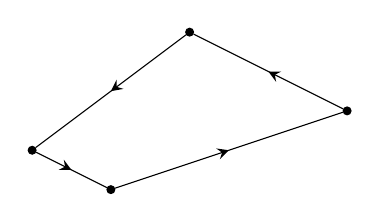
\begin{tikzpicture}
		\tikzset{vertex/.style = {shape=circle,draw, inner sep = 1pt, fill=black}}
		\tikzset{edge/.style = {arrowMe=stealth}}

		\node[vertex] (A) at (0,0) {};
		\node[vertex] (B) at (3,1) {};
		\node[vertex] (C) at (1,2) {};
		\node[vertex] (D) at (-1,0.5) {};

		\draw[edge] (A) to (B);
		\draw[edge] (B) to (C);
		\draw[edge] (C) to (D);
		\draw[edge] (D) to (A);
	\end{tikzpicture}
\end{center}

\noindent
\textit{Cyklem} w grafie skierowanym nazywamy taki ciąg krawędzi $e_1$, ..., $e_k$, że wierzchołek końcowy krawędzi $e_i$ jest wierzchołkiem początkowym krawędzi $e_{i + 1}$ dla każdego ${1 \leqslant i \leqslant n}$ -- przyjmujemy $e_{k + 1} = e_1$. Przykład cyklu znajduje się na drugim rysunku powyżej.

\vspace{5px}

\noindent
Dla każdego wierzchołka definiujemy \text{stopień wejściowy} jako liczbę krawędzi, które ,,wchodzą'' do danego wierzchołka i oznaczamy go symbolem $indeg(v)$. Analogicznie definiujemy \text{stopień wyjściowy} jako liczbę krawędzi, które ,,wychodzą'' z danego wierzchołka -- oznaczamy go jako $outdeg(v)$. Dla przykładowego grafu na rysunku powyżej i jego wierzchołka~$X$ mamy
\[
	indeg(x) = 3,  \quad outdeg(x) = 2.
\]


\vspace{10px}

\heading{Lemat 1}

\noindent
W grafie skierowanym, w którym dla każdego wierzchołka $v$ zachodzi 
\[
	out(v) \geqslant 1
\] 
istnieje cykl.

\vspace{5px}

\heading{Dowód}

\noindent
Rozpatrzmy dowolny wierzchołek $v_1$. Z warunków zadania istnieje krawędź wychodząca z niego. Przejdźmy nią do pewnego wierzchołka $v_2$. Kontynuujmy takie przechodzenie -- oznaczmy jako $v_i$ wierzchołek, który odwiedzimy jako $i$-ty. Jako, że wierzchołków jest skończenie wiele, to w pewnym momencie trafimy do wierzchołka, w którym już byliśmy. Załóżmy, że wierzchołek $v_{b + 1}$ jest tym samym wierzchołkiem co wierzchołek $v_a$. Wówczas wierzchołki
\[
	v_a, \; v_{a + 1}, \; v_{a + 2}, \; ..., \; v_{b - 1}, \; v_b
\]
tworzą cykl.

\qed

\newpage


%Source: https://www.comp.nus.edu.sg/~warut/cycles.pdf P1
\heading{Przykład 1}

\noindent
Pewne $n \geqslant 2$ osób zostało przydzielonych do $n$ pokoi, przy czym w każdym pokoju znajduje się dokładnie jedna osoba. Każda z osób ustaliła listę preferencji posortowała pokoje w pewnej kolejności. Wiadomo, że jeśli przyporządkowano by pokoje w inny sposób, to znalazła by się osoba, dla której nowy pokój był niżej na jej liście niż pierwotnie przyporządkowany jej pokój. Wykazać, że istnieje osoba, która ma na najwyższym miejscu swojej listy pokój, który został jej przyporządkowany.

\vspace{5px}

\heading{Rozwiązanie}

\noindent
Zadanie w treści nie zawiera słowa ,,graf''. Jednak czasami warto sobie taki graf stworzyć. Rozpatrzmy więc graf skierowany, który ma $n$ wierzchołków -- ponumerujmy je liczbami od $1$ do $n$. Jeśli osoba, której przyporządkowano pokój $i$ ma na najwyższym miejscy swojej listy preferencji pokój $j$, to graf będzie zawierał krawędź z $i$ do $j$. 

\vspace{5px}

\noindent
Załóżmy nie wprost, że szukana osoba nie istnieje -- tj. z każdego wierzchołka wychodzi dokładnie jedna krawędź. Wówczas na mocy Lematu $1$ w rozpatrywanym grafie istnieje cykl -- powiedzmy, że przechodzi przez wierzchołki
\[
	a_1, \; a_2, \; a_3, \; ..., \; a_k.
\]
Wówczas przydzielając osobie z pokoju $a_i$ pokój $a_{i + 1}$ dla każdego $1 \leqslant i \leqslant k$, gdzie $a_{k + 1} = a_1$, otrzymamy przyporządkowanie, w którym każda osoba otrzyma subiektywnie lepszy pokój niż wcześniej. Jest to jednak sprzeczne z założeniami.

\qed

\heading{Turnieje}

\noindent
Zdarza się, że w zadaniu są rozpatrywane pewne zawody, w których wzięła udział pewna liczba graczy, każda para rozegrała mecz, który zakończył się zwycięstwem jednej ze stron. Możemy wówczas rozpatrzyć graf skierowany, w którym wierzchołki będą odpowiadały graczom. Pomiędzy każdą dwójką graczy będzie występowałą dokładnie jedna krawędź i będzie ona skierowana w stronę zwycięzcy. Taki graf nazywamy $\textit{turniejem}$ -- przykład znajduje się na rysunku.

\begin{center}
	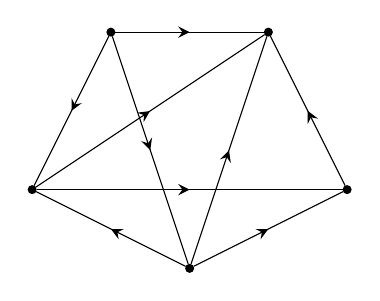
\begin{tikzpicture}
		\tikzset{vertex/.style = {shape=circle,draw, inner sep = 1pt, fill=black}}
		\tikzset{edge/.style = {arrowMe=stealth}}

		\node[vertex] (A_1) at (0,0) {};
		\node[vertex] (A_2) at (2,1) {};
		\node[vertex] (A_3) at (1,3) {};
		\node[vertex] (A_4) at (-2,1) {};
		\node[vertex] (A_5) at (-1,3) {};

		\draw[edge] (A_1) to (A_2);
		\draw[edge] (A_2) to (A_3);
		\draw[edge] (A_1) to (A_4);
		\draw[edge] (A_5) to (A_1);
		\draw[edge] (A_4) to (A_2);
		\draw[edge] (A_1) to (A_3);
		\draw[edge] (A_4) to (A_3);
		\draw[edge] (A_5) to (A_4);
		\draw[edge] (A_5) to (A_3);
	\end{tikzpicture}
\end{center}

\noindent
Turniej nazwiemy \textit{redukowalnym}, gdy możemy podzielić jego uczestników na dwa niepuste zbiory $A$ oraz $B$, takie, że każdy uczestnik z $A$ wygrał z każdym uczestnikiem z $B$. Przykład takiego turnieju narysowano poniżej po lewej stronie.

\begin{center}
	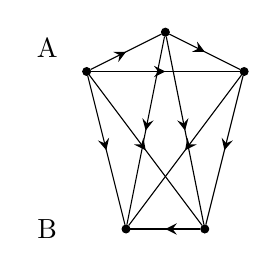
\begin{tikzpicture}
		\tikzset{vertex/.style = {shape=circle,draw, inner sep = 1pt, fill=black}}
		\tikzset{edge/.style = {arrowMe=stealth}}

		\node[vertex] (A_1) at (1,2) {};
		\node[vertex] (A_2) at (2,2.5) {};
		\node[vertex] (A_3) at (3,2) {};
		\node[vertex] (B_1) at (1.5,0) {};
		\node[vertex] (B_2) at (2.5,0) {};

		\draw[edge] (A_1) to (A_2);
		\draw[edge] (A_2) to (A_3);
		\draw[edge] (A_1) to (A_3);

		\draw[edge] (A_1) to (B_1);
		\draw[edge] (A_2) to (B_1);
		\draw[edge] (A_3) to (B_1);
		\draw[edge] (A_1) to (B_2);
		\draw[edge] (A_2) to (B_2);
		\draw[edge] (A_3) to (B_2);


		\draw[edge] (B_2) to (B_1);



		\node (x) at (0.5,2.3) {A};
		\node (x) at (0.5,0) {B};
	\end{tikzpicture}
	\hspace{80px}
	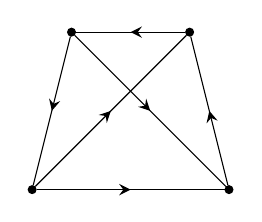
\begin{tikzpicture}
		\tikzset{vertex/.style = {shape=circle,draw, inner sep = 1pt, fill=black}}
		\tikzset{edge/.style = {arrowMe=stealth}}

		\node[vertex] (A_1) at (0,0) {};
		\node[vertex] (A_2) at (2.5,0) {};
		\node[vertex] (A_3) at (2,2) {};
		\node[vertex] (A_4) at (0.5,2) {};

		\draw[edge] (A_1) to (A_2);
		\draw[edge] (A_2) to (A_3);
		\draw[edge] (A_3) to (A_4);
		\draw[edge] (A_4) to (A_1);
		\draw[edge] (A_1) to (A_3);
		\draw[edge] (A_4) to (A_2);


	\end{tikzpicture}
\end{center}

\noindent
Turniej nazwiemy \textit{cyklicznym}, gdy istnieje w nim cykl, który przechodzi przez każdy wierzchołek dokładnie raz. Przykład takiego turnieju znajduje się po prawej stronie powyższego rysunku.

\vspace{10px}
\noindent
Zachęcamy do samodzielnego zmierzenia się z poniższymi Lematami.

\vspace{10px}

\heading{Lemat 2}

\noindent
Turniej jest redukowalny wtedy i tylko wtedy, gdy nie jest cykliczny.

\vspace{5px}

\heading{Dowód}

\noindent
Zauważmy, że jeśli turniej jest redukowalny, to nie może on zawierać żadnego cyklu. Graf ten wówczas da się podzielić na dwie części $A$ oraz $B$, takie, że każdy uczestnik z $A$ wygrał z każdym uczestnikiem z $B$. Załóżmy, że istnieje pewien cykl $v_1, \; v_2, \;, ..., \; v_k$. Wówczas część jego wierzchołków należy do $A$, a reszta do $B$. Stąd istnieje takie $i$, że $v_i$ należy do~$B$, a $v_{i + 1}$ należy do $A$. Jednak wówczas $v_{i + 1}$ wygrałby z $v_i$, co daje sprzeczność.

\vspace{10px}
\noindent
Przejdźmy teraz do trudniejszej części -- tj. wykazania, że jeśli graf nie jest cykliczny, to jest redukowalny. Rozpatrzmy największy cykl
\[
	v_1, \; v_{2}, \; v_{3}, \; ..., \; v_k
\]
w danym grafie. Skoro graf ten nie jest cykliczny, to istnieje pewien wierzchołek $x$ spoza cyklu.

\vspace{10px}
\noindent
\underline{Obserwacja 1.} Jeśli $x$ jest wierzchołkiem spoza cyklu, to albo $x$ przegrał z~wszystkimi \phantom{Obserwacja 1.  }~wierzchołkami z cyklu, albo $x$ wygrał z wszystkimi wierzchołkami z cyklu.

\begin{center}
	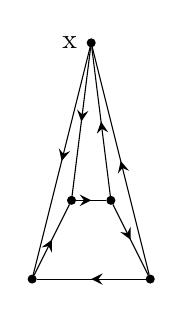
\begin{tikzpicture}
		\tikzset{vertex/.style = {shape=circle,draw, inner sep = 1pt, fill=black}}
		\tikzset{edge/.style = {arrowMe=stealth}}

		\node[vertex, label=left:x] (X) at (0.75,3) {};
		\node[vertex] (A_1) at (0,0) {};
		\node[vertex] (A_2) at (0.5,1) {};
		\node[vertex] (A_3) at (1,1) {};
		\node[vertex] (A_4) at (1.5,0) {};


		\draw[edge] (A_1) to (A_2) {};
		\draw[edge] (A_2) to (A_3) {};
		\draw[edge] (A_3) to (A_4) {};
		\draw[edge] (A_4) to (A_1) {};


		\draw[edge] (X) to (A_1) {};
		\draw[edge] (X) to (A_2) {};
		\draw[edge] (A_3) to (X) {};
		\draw[edge] (A_4) to (X) {};

	\end{tikzpicture}
\end{center}

\vspace{10px}
\noindent
Załóżmy, że $x$ przegrał z niektórymi wierzchołkami z cyklu, a z niektórymi wygrał. Wówczas istnieje takie $i$, że $x$ wygrał z $v_{i + 1}$, a przegrał z $v_{i}$ -- oczywiście przyjmujemy $v_{k + 1} = v_{1}$. Wówczas wierzchołki
\[
	v_1, \; v_{2}, \; ..., \; v_i, \; x, \;, v_{i + 1}, \; ..., \; v_k
\]
tworzyłyby cykl, co przeczy założonej maksymalności cyklu wyjściowego.



\vspace{10px}
\noindent
Możemy więc podzielić wierzchołki na trzy grupy:
\begin{itemize}
	\item grupę $A$ -- wierzchołków spoza rozpatrywanego cyklu, które wygrały z każdym z wierzchołków z cyklu,
	\item grupę $B$ -- wierzchołków spoza rozpatrywanego cyklu, które przegrały z każdym z wierzchołków z cyklu,
	\item grupę $C$ -- wierzchołki z rozpatrywanego cyklu.
\end{itemize}

\vspace{10px}
\noindent
\underline{Obserwacja 2.} Jeśli $x$ należy do grupy $A$, a $y$ do grupy $B$, to $x$ wygrał z $y$.

\begin{center}
	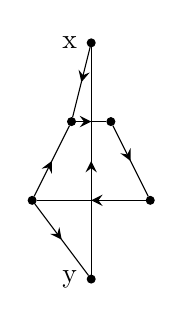
\begin{tikzpicture}
		\tikzset{vertex/.style = {shape=circle,draw, inner sep = 1pt, fill=black}}
		\tikzset{edge/.style = {arrowMe=stealth}}

		\node[vertex, label=left:x] (X) at (0.75,2) {};
		\node[vertex, label=left:y] (Y) at (0.75,-1) {};
		\node[vertex] (A_1) at (0,0) {};
		\node[vertex] (A_2) at (0.5,1) {};
		\node[vertex] (A_3) at (1,1) {};
		\node[vertex] (A_4) at (1.5,0) {};


		\draw[edge] (A_1) to (A_2) {};
		\draw[edge] (A_2) to (A_3) {};
		\draw[edge] (A_3) to (A_4) {};
		\draw[edge] (A_4) to (A_1) {};


		\draw[edge] (A_1) to (Y) {};
		\draw[edge] (Y) to (X) {};
		\draw[edge] (X) to (A_2) {};

	\end{tikzpicture}
\end{center}


\vspace{10px}
\noindent
Załóżmy nie wprost, że $y$ wygrał z $x$. Wówczas wierzchołki
\[
	v_1, \; y, \; x, \; v_{2}, \; ..., \; v_k, 
\]
tworzyłyby większy cykl -- sprzeczność.

\vspace{10px}
\noindent
Skoro nie wszystkie wierzchołki należą do do grupy $C$, to istnieje inna grupa, która jest niepusta -- przyjmijmy bez straty ogólności, że jest to grupa $A$. Wówczas podział na zbiory $A \cup C$ oraz $B$ dowodzi redukowalności grafu.

\qed


\heading{Lemat 3}

\noindent
Jeśli turniej o $n \geqslant 4$ wierzchołkach jest cykliczny, to zawiera cykl o długości równiej $n - 1$.

\vspace{5px}

\heading{Dowód}

\noindent
Usuńmy pewien wierzchołek $x$. Otrzymany graf zawiera $n - 1$ wierzchołków, więc jeśli jest cykliczny, to wynika z tego teza. Załóżmy więc, że tak nie jest -- na mocy Lematu~$2$ jest on redukowalny. Niech więc rozpatrywany graf składa się z wierzchołka $x$ oraz niepustych zbiorów wierzchołków $A$ oraz $B$, przy czym każdy wierzchołek z $A$ wygrał z każdym wierzchołkiem z $B$.

\vspace{10px}
\noindent
Skoro rozpatrywany graf jest cykliczny, to istnieje cykl
\[
	x, \; v_1, \;, v_2, \; ...,\; v_{n - 1}.
\]
Zauważmy, że jeśli $v_{i + 1}$ należy do $A$, to jako, że $v_{i}$ wygrało z $v_{i + 1}$, to nie może należeć ono do $B$. Stąd również należy do $A$. Stąd też istnieje takie $t$, że
\[
	v_1, \;, v_2, \; ...,\; v_{t} \in A, \quad v_t, \;, v_{t + 1}, \; ...,\; v_{n - 1} \in B.
\]

\begin{center}
	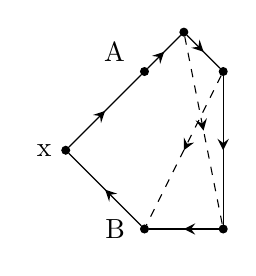
\begin{tikzpicture}
		\tikzset{vertex/.style = {shape=circle,draw, inner sep = 1pt, fill=black}}
		\tikzset{edge/.style = {arrowMe=stealth}}

		\node[vertex, label=left:x] (X) at (-1,1) {};

		\node[vertex] (A_1) at (0,2) {};
		\node[vertex] (A_2) at (0.5,2.5) {};
		\node[vertex] (A_3) at (1,2) {};
		\node[vertex] (B_1) at (1,0) {};
		\node[vertex] (B_2) at (0,0) {};
		\node[label=left:A] (a) at (0,2.25) {};
		\node[label=left:B] (b) at (0,0) {};


		\draw[edge] (X) to (A_1) {};
		\draw[edge] (A_1) to (A_2) {};
		\draw[edge] (A_2) to (A_3) {};
		\draw[edge] (A_3) to (B_1) {};
		\draw[edge] (B_1) to (B_2) {};
		\draw[edge] (B_2) to (X) {};


		\draw[edge, dashed] (A_3) to (B_2) {};
		\draw[edge, dashed] (A_2) to (B_1) {};

	\end{tikzpicture}
\end{center}

\noindent
Jeśli $t \geqslant 2$, to oznacza, że istnieje $v_{t - 1}$. Skoro $v_{t - 1} \in A$ oraz $v_{t + 1} \in B$, to $v_{t - 1}$ wygrał~z~$v_{t + 1}$. Czyli
\[
	x, \; v_1, \;, v_2, \; ..., \;, v_{t - 1}, \; v_{t + 1}, \; ..., \; v_{n - 1}
\]
jest cyklem o długości $n - 1$. Jeśli zaś $t = 1$, to $t + 2 = 3 \leqslant n - 1$. Analogicznie jak powyżej wykazujemy, że $v_{t}$ wygrał z $v_{t + 2}$, czyli
\[
	x, \; v_1, \;, v_2, \; ..., \;, v_{t}, \; v_{t + 2}, \; ..., \; v_{n - 1}
\]
jest cyklem o długości $n - 1$.

\qed
%Source:
\begin{problem}{1}

\end{problem}


\newpage
% Rozdział 16 – ciągi

\theory{Ciągi}

\noindent
Ciągiem $(a_n)_{n \geqslant 0}$ nazywamy funkcję ze zbioru liczb nieujemnych całkowitych w zbiór liczb rzeczywistych. Innymi słowy każdemu indeksowi $i$ jest przyporządkowana pewna liczba rzeczywista $a_i$. Najbardziej znanym przykładem ciągu jest \textit{ciąg Fibonacciego}. Jest on dany wzorem
\[
	F_0 = 0, \quad F_1 = 1, \quad F_{n + 2} = F_{n + 1} + F_{n} \text{ dla } n \geqslant 0.
\]
Można obliczyć, że
\[
	F_2 = 1, \; F_3 = 2, \; F_4 = 3, \; F_5 = 5, \; F_6 = 8, \; F_7 = 13, \; F_8 = 21, \; F_9 = 34, \; ...
\]
Zauważmy, że każdy kolejny wyraz tego ciągu jest zależny od poprzedzających go elementów. Ciągi tak zdefiniowane nazywamy \textit{ciągami rekurencyjnymi}. Można jednak wyznaczyć wzór na każdy element ciągu Fibonacciego, który nie jest rekurencyjny -- zależy tylko od indeksu danego elementu ciągu. Wyprowadzenie tego wzoru jest bardzo pomysłowe i zastosowanie podobnego postępowania pozwala na wyprowadzenie wzoru ogólnego wielu innych ciągów rekurencyjnych.

\vspace{10px}

\heading{Wzór ogólny na wyrazy ciągu Fibonacciego}

\noindent
Zapomnijmy na chwilę o warunkach $F_0 = 0, \; F_1 = 1$ i spróbujmy znaleźć jakieś ciągi, dla których również zachodzi równanie rekurencyjne $a_{n + 2} = a_{n + 1} + a_n$, ale mają one prosty do wyprowadzenie wzór ogólny. Zobaczmy na ciągi dane wzorem $a_n = x^n$ dla pewnej liczby rzeczywistej $x$ -- być może dla pewnej liczby rzeczywistej $x$ będą one spełniały postulowane równanie rekurencyjne. Przyjmuje ono postać
\begin{align*}
	x^{n + 2} &= x^{n + 1} + x^n, \\
	x^2 &= x + 1.
\end{align*}
Rozwiązując powyższe równanie kwadratowe możemy dojść do wniosku, że ciągi 
\[
	a_n = \alpha^n, \text{ gdzie } \alpha = \frac{1 + \sqrt{5}}{2} \quad \text{i} \quad a_n = \beta^n,  \text{ gdzie } \beta = \frac{1 - \sqrt{5}}{2} 
\] 
spełniają daną rekurencję.

\vspace{10px}
\noindent
Zauważmy, że dla dowolnych liczb rzeczywistych $A$ oraz $B$ ciąg
\[
	c_n = Aa_n + Bb_n
\]
również będzie spełniał rekurencję $c_{n + 2} = c_{n + 1} + c_n$. Istotnie
\begin{align*}
	c_{n + 2} &= Aa_{n + 2} + Bb_{n + 2} = A(a_{n + 1} + a_n) + B(b_{n + 1} + b_n) = \\
	&= (Aa_{n + 1}  + Bb_{n + 1}) + (Aa_n + Bb_n) = c_{n + 1} + c_n.
\end{align*}
Postaramy się poruszać liczbami $A$ oraz $B$, tak, by ciąg $c_n$ spełniał równości
\[
	c_{0} = F_0 = 0, \; c_{1} = F_1 = 1.
\]
Wówczas, co nietrudno zauważyć, ciągi $F$ i $c$ będą sobie równe. W tym celu wystarczy rozwiązać układ równań
\[
	\begin{cases}
		Aa_0 + Bb_0 = A + B = 0 \\
		Aa_1 + Bb_1 = \alpha \cdot A + \beta \cdot B = 1.
	\end{cases}
\]
Powyższe równości zachodzą dla $A = \frac{1}{\sqrt{5}}$ i $B = -\frac{1}{\sqrt{5}}$. Toteż otrzymujemy zależność
\[
	F_n = c_n = \frac{1}{\sqrt{5}} \cdot a_n - \frac{1}{\sqrt{5}} \cdot b_n = \frac{\alpha^n - \beta^n}{\sqrt{5}}.
\]

\heading{Przykład 1}

\noindent
Wykazać, że dla każdej liczby całkowitej $M > 1$ istnieje taka dodatnia liczba całkowita~$n$, że $F_n$ jest podzielne przez $M$.

\vspace{5px}

\heading{Rozwiązanie}

\noindent
Najpierw wykażemy, że ciąg reszt z dzielenia liczb $F_n$ przez $M$ jest okresowy. Reszt z~dzielenia przez $M$ jest skończenie wiele. Również liczba wartości jakie może przyjąć para $(F_i \pmod{M},\; F_{i + 1}\pmod{M})$ jest skończona. Toteż istnieją takie liczby $i < j$, dla których
\[
	F_i \equiv F_j \pmod{M} \quad \text{oraz} \quad F_{i + 1} = F_{j + 1} \pmod{M}.
\]
Możemy zauważyć, że
\[
	F_{j + 2} \equiv F_{j + 1} + F_j \equiv F_{i + 1} + F_i \equiv F_{i + 2} \pmod{M}.
\]
Kontynuując to rozumowanie można wykazać, że $F_{i + k} \equiv F_{j + k} \pmod{M}$ dla dowolnej liczby całkowitej dodatniej $k$.
Możemy się również ,,cofać'', to jest
\[
	F_{j - 1} \equiv F_{j + 1} - F_j \equiv F_{i + 1} - F_i \equiv F_{i - 1} \pmod{M}.
\]
i w ten sposób wykazać, że $F_{i + k} \equiv F_{j + k} \pmod{M}$ również zachodzi dla dowolnej liczby całkowitej ujemnej $k$. Otrzymaliśmy więc, że
\begin{align*}
	F_{i + k} \equiv F_{j + k} &\pmod{M}\\
	F_{k} \equiv F_{k + (j - i)} &\pmod{M} \\
	F_{k} \equiv F_{k + t} &\pmod{M},
\end{align*}
dla pewnej dodatniej liczby całkowitej $t$.

\vspace{10px}

\noindent
Zauważmy, że $F_0 \equiv 0 \pmod{M}$. Wówczas
\[
	0 \equiv F_0 \equiv F_t \equiv F_{2t} \equiv F_{3t} \equiv ... \pmod{M},
\]
co kończy dowód.

\qed

\noindent
Przykładowo dla $M = 4$ ciąg reszt $F_n$ z dzielenia przez $M$ wygląda następująco
\[
	0,\; 1,\; 1,\; 2,\; 3,\; 1,\; 0,\; 1,\; 1,\; 2,\; ...
\]

\heading{Przykład 2}

\noindent
Znajdź wszystkie liczby całkowite $n \geq 3$, dla których istnieją liczby rzeczywiste $a_1, a_2, \dots a_{n + 2}$ spełniające $a_{n + 1} = a_1$, $a_{n + 2} = a_2$ oraz
\[
	a_ia_{i + 1} + 1 = a_{i + 2},
\]
dla $i = 1, 2, \dots, n$.


\newpage
\heading{Rozwiązanie}

\noindent
W tego typu zadaniach zawsze warto sprawdzić co się dzieje dla niewielkich liczb $n$. Czytleniczce/czytelnikowi pozostawiamy jako ćwiczenie zobaczenie, że w przypadkach $n = 1$ i $n = 2$ szukany ciąg nie istnieje. Dla $n = 3$ otrzymamy układ równań
\[
	\begin{cases}
		a_1a_2 + 1 = a_3, \\
		a_2a_3 + 1 = a_1, \\
		a_3a_1 + 1 = a_2.
	\end{cases}
\]
Metodą zgadywania można sprawdzić, że $a_1 = a_2 = - 1, a_3 = 2$ spełnia warunki zadania. Czytelniczka/czytelnik może zadać pytanie, jak zgadywać takie rzeczy. Warto podstawić sobie kolejno $a_1 = 1, 0, -1$ i zobaczyć co z tego wynika. Jeśli każde z tego typu prostych podstawień doprowadza do sprzeczności, to można postawić hipotezę, że układ nie ma rozwiązań. Niemniej jednak w tym przypadku takie rozwiązania istnieją.

\vspace{10px}
\noindent
Można łatwo zauważyć, że skoro dla $n = 3$ szukany ciąg istnieje, to takowy będzie istniał również dla $n = 3k$ dla dowolnej liczby dodatniej całkowitej $k$. Wystarczy bowiem rozpatrzyć ciąg postaci
\[
	(a_1, \; a_2, \; a_3, \; a_1, \; a_2, \; a_3, \; ..., \; a_1, \; a_2, \; a_3).
\]

\vspace{10px}
\noindent
Rozpatrzmy ciąg $(a_n)$ spełniający warunki zadania. Mamy
\[
	a_ia_{i + 1} + 1 = a_{i + 2},
\]
\[
	a_ia_{i + 1}a_{i + 2} + a_{i + 2} = a_{i + 2}^2,
\]
\[
	\sum_{i = 1}^{n} a_ia_{i + 1}a_{i + 2} + \sum_{i = 1}^{n} a_{i + 2} = \sum_{i = 1}^{n} a_{i + 2}^2.
\]
W podobny sposób otrzymujemy
\[
	a_ia_{i + 1} + 1 = a_{i + 2},
\]
\[
	a_{i - 1}a_ia_{i + 1} + a_{i - 1} = a_{i + 2}a_{i - 1},
\]
\[
	\sum_{i = 1}^{n} a_{i - 1}a_ia_{i + 1} + \sum_{i = 1}^{n} a_{i - 1} = \sum_{i = 1}^{n} a_{i + 2}a_{i - 1}.
\]
Pozostaje zauważyć, że
\[
	\sum_{i = 1}^{n} a_{i - 1} = \sum_{i = 1}^{n} a_{i + 2} \quad \text{i} \quad \sum_{i = 1}^{n} a_{i - 1}a_ia_{i + 1} = \sum_{i = 1}^{n} a_ia_{i + 1}a_{i + 2},
\]
gdyż jest to sumowanie tych samych liczb, tylko w innej kolejności. Mamy więc równość
\[
	\sum_{i = 1}^{n} a_{i + 2}^2 = \sum_{i = 1}^{n} a_{i + 2}a_{i - 1}.
\]
Zauważmy, że $\sum_{i = 1}^{n} a_{i + 2}^2 = \sum_{i = 1}^{n} a_{i - 1}^2$, skąd
\begin{align*}
	\sum_{i = 1}^{n} \left(a_{i + 2}^2 + a_{i - 1}^2 - 2a_{i + 2}a_{i - 1}\right) = 0, \\
	\sum_{i = 1}^{n} \left(a_{i + 2} - a_{i - 1}^2\right)^2 = 0.
\end{align*}
Otrzymujemy stąd, że $a_{i - 1} = a_{i + 2}$, czyli $a_i = a_{i + 3}$. Jeśli $n$ jest niepodzielne przez $3$, to w ciągu równości
\[
	a_1 = a_4 = a_7 = ...
\]
pojawią się wszystkie elementy ciągu, toteż wszystkie muszą być równe. Ale jeśli ${a_1 = a_2 = a_3}$, to
\[
	a_1^2 + 1 = a_1,
\]
co nie ma rozwiązań. Stąd też jeśli $n$ nie jest liczbą podzielną przez $3$ to szukany ciąg nie istnieje. Łącząc to z początkową obserwacją mamy, że szukany ciąg istnieje wtedy i tylko wtedy, gdy liczba $n$ jest podzielna przez $3$.

\qed

\noindent
Powyższe zadanie ma dwa pouczające przesłania. Po pierwsze pokazuje, jak często rozważanie małych przypadków naprowadza na postawienie poprawnych hipotez. Po drugie, warto czasami po prostu nieco pobawić się tożsamościami algebraicznymi, gdyż można dojść w ten sposób do ciekawych wniosków. Może wydawać się, że to rozwiązania wynika znikąd, no ale czasem tak po prostu jest -- trzeba takich rzeczy też poszukać.

\vspace{10px}
%Source:
\begin{problem}{1}

\end{problem}


\headingpage{Podpowiedzi 1}
\addcontentsline{toc}{section}{Podpowiedzi 1}
%--------------------------- Hint 1 ---------------------%

\newpage
\hints{Indukcja matematyczna}

\begin{hints_list}
	\item Przeprowadź rozumowanie indukcyjne po liczbie wierzchołków $n$.

	\item Sprawdź, że równość zachodzi dla $n = 1$. Załóż, że równość zachodzi dla $n$ i spróbuj wykazać ją dla $n + 1$.

	\item
	Przeprowadź indukcję po liczbie $n$. Skorzystaj dla wszystkich początkowych dysków poza najniżej położonym.

	\item Rozpatrz $n + 1$ punktów i zobacz co się stanie jeśli usuniemy jeden z nich.

	\item Spróbuj wykazać tezę inducją po $n$. Aby to zrobić, trzeba będzie wykazać indukcyjnie inną równość pomocniczą.

	\item Spróbuj podzielić planszę $2^{n + 1} \cdot 2^{n + 1}$ na kilka części.

	\item Zastosuj indukcję co 2.
\end{hints_list}
\hints{Równania funkcyjne}

\begin{hints_list}
	\item Podstaw $y = 0$.
	\item Przyjmij $x = f(y)$.
	\item Wykaż, że $f(0) = 0$.
	\item Podstaw $1 - x$ pod $x$.
	\item Skorzystaj z danego równania dla $x = 0$.
	\item Podstaw $y = -x$.
	\item Przyjmij $x = 0$.
	\item Podstaw $f(x)$ w miejsce $x$.
	\item Podstaw: $x = y = 0$ oraz $x = y$.
	\item Wykaż, że $f$ jest różnowartościowa.
\end{hints_list}
\hints{Równania funkcyjne}

\begin{hints_list}
	\item Podstaw $y = 0$.
	\item Przyjmij $x = f(y)$.
	\item Wykaż, że $f(0) = 0$.
	\item Podstaw $1 - x$ pod $x$.
	\item Skorzystaj z danego równania dla $x = 0$.
	\item Podstaw $y = -x$.
	\item Przymij $x = 0$.
	\item Podstaw $f(x)$ w miejsce $x$.
	\item Podstaw: $x = y = 0$ oraz $x = y$.
	\item Wykaż, że $f$ jest różnowartościowa.
\end{hints_list}
\hints{Równania funkcyjne}

\begin{hints_list}
	\item 
\end{hints_list}
\hints{Nierówności między średnimi}

\begin{hints_list}
	\item Skorzystaj z AM-GM dla trzech liczb.
	\item Przeszacuj każdy z nawiasów z osobna.
	\item Przekształć nierówność zanim skorzystasz ze średnich.
	\item Zauważ, że $a^2 \geqslant 2a - 1$.
	\item Dodaj coś do obu stron, aby prawa strona równości była ładna.
\end{hints_list}
\hints{Konstrukcje}

\begin{hints_list}
	\item Niech pokolorowane pola tworzą kwadrat.
	\item Podziel płaszczyznę na kratki.
	\item Podziel trójkąt na mniej takich czworokątów.
	\item Rozpatrz rozkłady na czynniki pierwsze.
	\item Rozpatrz planszę $7\times7$, na której każde pole reprezentuje pewną osobę.
	\item Spróbuj rozwiązać zadania dla $a + 1$ i $a + 2$.
\end{hints_list}
\hints{Wielomiany}

\begin{hints_list}
	\item Załóż nie wprost, że istnieje pewne niecałkowite $\alpha$, że $W(\alpha) = 0$.
	\item Rozpatrz wielomian o pierwiastkach $a$, $b$ i $c$.
	\item Wykaż, że dla każdej dodatniej liczby całkowitej $n$ wielomian $x^{3n - 1} + x + 1$ jest podzielny przez wielomian $x^2 + x + 1$.
	\item Przeprowadź indukcję po stopniu $P$.
	\item Rozpatrz wielomian $Q(x) = W(x) - 5$.
	\item Taki wielomian nie istnieje. Skorzystaj z podobnego pomysłu co we wzorach Viete'a w części teoretycznej.
\end{hints_list}
\hints{Wielomiany}

\begin{hints_list}
	\item Rozpatrz najdłuższą ścieżkę w grafie i spróbuj ją wydłużyć.
	\item Skorzystaj z indukcji matematycznej.
	\item Rozpatrz graf, w którym wierzchołkami będą drużyny. Połączymy je czerwoną krawędzią, gdy grały mecz pierwszego dnia, zieloną, gdy drugiego.
	\item Wykaż, że mając pewien graf z pewnym kolorowaniem, to wybierając dwa dowolne wierzchołki $u$ oraz $v$ jesteśmy w stanie zmienić parzystość liczby kolorowych krawędzi wychodzących z nich, nie naruszając tej liczby dla innych wierzchołków.
	\item Wybierz jeden wierzchołek, następnie usuń wszystkich jego sąsiadów. Powtarzaj taki krok z otrzymanym grafem, aż wszystkie wierzchołki zostaną usunięte. Wybierając mądrze wierzchołki możemy zrobić to tak, że wybierzemy ich odpowiednio dużo.
	\item Odpowiedzią jest $N = 10$.
\end{hints_list}
\hints{Indukcja matematyczna 2}

\begin{hints_list}
	\item Zauważ, że jeśli kwotę $k$ złotych da się opłacić w szukany sposób, to kwotę $k + 3$ również.
	\item Rozpatrz punkty $(a, b)$, dla których zachodzi równość $a + b = n + 1$.
	\item Spróbuj rozwiązać zadanie dla liczb podzielnych przez $2$, $4$, i $8$.
	\item Usuń pewien specyficzny wierzchołek i zastosuj założenie indukcyjne.
	\item Wstaw $n = 1$. Wykaż, że $f(n) = n$ korzystając z indukcji zupełnej po $n$.
	\item Wykaż ogólniejszą tezę:
	Niech $\mathcal{R}$ będzie rodziną zbiorów $n$-elementowych. Moc $\mathcal{R}$ jest większa niż $n! \cdot k^{n}$ Wówczas istnieje $k+1$-elementowa rodzina $\mathcal{G}$, będąca podrodziną $\mathcal{R}$, oraz taki zbiór $X$, że dla dowolnych zbiorów $A, B \in \mathcal{R}$ zachodzi $A \cap B = X$.
\end{hints_list}
\hints{Podzielności}

\begin{hints_list}
	\item Rozpatrz największą liczbę całkowitą $k$, że $n \geqslant k^2$.
	\item Zamień wszystkie założenia i tezę na wyrażenia związane z $v_p$.
	\item Załóż nie wprost, że jeśli $d$ i $d + 2$ są dzielnikami $4n$, to liczba $d + 1$ również.
	\item Wykaż, że $a + 1 \mid b + 1$.
	\item Wykaż, że $a$ i $b$ dają tę samą resztę z dzielenia przez $p$.
	\item Załóż, że $v_p(a)$ nie jest podzielne przez $k$. Weź odpowiednie $n$, aby uzyskać sprzeczność.
\end{hints_list}
\hints{Gry}

\begin{hints_list}
	\item Zawsze da się uzyskać $1$. Wykazać, że da się, być może w kilku ruchach, zmniejszyć zapisaną na tablicy liczbę.
	\item Analizuj pola tabeli $m \times n$ jako stany wygrywające i przegrywające.
	\item Wykaż, że liczby parzyste są wygrywające.
	\item Podziel planszę na pewne figury. Rozważ strategię, która każde drugiemu graczowi stawiać swój znak w tej samej figurze, w której postawił go gracz pierwszy.
	\item Niech dla pewnej liczby $n$ w pierwszych $4n$ ruchach nauczyciel narysuje kwadrat o boku $n$.
	\item Przyjmijmy, że na każdym kamieniu są miejsca na zapisanie dwóch liczb. Jeśli pewna dziewczyna $a$ przekaże dziewczynie $b$ kamień po raz pierwszy, to o ile na kamieniu nie jest nic zapisane, to zapisuje się tam numery $a$ i $b$.  Jeśli pewna dziewczyna musi przekazać kamień swojej sąsiadce, to jeśli dysponuje kamieniem z zapisanymi numerami swoimi i sąsiadki, to przekaże jej właśnie go. Zobacz, co z tego wynika.
\end{hints_list}
\hints{Bardziej zaawansowane nierówności}

\begin{hints_list}
	\item Skorzystaj z nierówności Schwarza w formie Engela.
	\item Rozpatrzmy ciągi $(a^2, b^2, c^2)$ oraz $bc, ac, ab$.
	\item Przyda się jedynka trygonometryczna, jak i fakt, że sinus i cosinus przyjmują wartości o module mniejszym od 1.
	\item Skorzystaj z nierówności o ciągach jednomonotonicznych.
	\item Zobacz co się stanie, gdy podstawisz $a = 0$.
\end{hints_list}
\hints{Równania funkcyjne i wielomianowe}

\begin{hints_list}
	\item Wykaż, że $f(f(0)) = 0$ oraz, że jeśli $f(f(a)) = 0$, to $a = 0$.
	\item Udowodnij, że $f(1) = 2$.
	\item Zauważ, że da się podstawić takie $y$, aby $f(x^2 + y) = f(x^{27} + 2y)$.
	\item Niech $d(n)$ oznacza liczbę dzielników. Wykaż, że $d(f(n)) = f(d(n))$.
	\item Podstaw $x = 0$. Wykaż, że $f$ jest różnowartościowa i że przyjmuje wszystkie wartości rzeczywiste.
	\item Niech $f$ będzie różnowartościową funkcją, która przyjmuje wszystkie wartości rzeczywiste poza zerem.
\end{hints_list}
\hints{Twierdzenia z teorii liczb}

\begin{hints_list}
	\item Zauważ, że jeśli $d$ dzieli $n$, to $\frac{n}{d}$ również dzieli $n$.
	\item Taka liczba istnieje.
	\item Rozpatrz liczby postaci $a^k$.
	\item Sprawdź dla małych $p$ ile ta suma wynosi.
	\item Użyj generatorów modulo $p$.
	\item Wykaż, że jedna spośród liczb od $1$ do $b_1b_2\cdot ... \cdot b_n$ spełnia warunki zadania.
\end{hints_list}
\hints{Grafy skierowane}

\begin{hints_list}
	\item Ponumeruj wierzchołki od $1$ do $n$. Usuń wszystkie krawędzie, dla których wierzchołek początkowy ma mniejszy numer niż końcowy. Co się wówczas stanie?
	\item Zauważ, że teza dla grafu cyklicznego jest trywialna.
	\item Rozpatrz taki podział, w którym liczba krawędzi, mających dwa końce w jednym zbiorze jest minimalna.
	\item Zauważ, że $A_k$ oraz $A_{k + 1}$ zdobyli razem co najmniej $999$ punktów. Wykaż, że jeśli zdobyli ich co najmniej $1000$, to łączna liczba punktów zdobyta przez wszystkich graczy nie będzie się zgadzać.
	\item Każda z osób musiała zdobyć $\frac{n - 1}{2}$ punktów.
	\item Usuń z grafu tyle krawędzi, aby nie było żadnego cyklu i liczba usuniętych krawędzi była najmniejsza możliwa.
\end{hints_list}
\hints{Ciągi}

\begin{hints_list}
	\item Jeśli przemnożymy wszystkie wyrazy ciągu arytmetycznego przez $k$, to co się stanie?
	\item Odpowiedź wynosi $n(n + 1)$.
	\item Znajdź wzór na $u_n$. Spróbuj policzyć $u_n$ dla małych $n$.
	\item Znajdź wzór ogólny na $a_n$.
	\item Podnieś równanie rekurencyjne do kwadratu stronami.
	\item Zauważ, że liczba pod pierwiastkiem musi być dodatnia.
	\item Wykaż również, że jeśli dla pewnej liczby całkowitej~$n$ zachodzi nierówność $\mathrm{NWD}(n, a_{n - 1}) > 1$, to $a_n = 3n$.
\end{hints_list}

\headingpage{Podpowiedzi 2}
\addcontentsline{toc}{section}{Podpowiedzi 2}
%--------------------------- Hint 2 ---------------------%

\newpage
\hints{Indukcja matematyczna}

\begin{hints_list}

	\item Rozpatrz trójkąt tworzony przez trzy kolejne wierzchołki $n$-kąta.

	\item Odejmij stronami tezę zadania dla $n + 1$ i $n$.

	\item Z założenia indukcyjnego możemy przenieść wszystkie dyski, poza najniżej położonym, na drugą igłę. Należy zauważyć, że dysk, którego nie używamy, nie przeszkodzi w wykonaniu takiego przełożenia.

	\item Co mówi założenie indukcyjne? Rozpatrz przypadek, gdy z usuniętego punktu wychodzą krawędzie różnych kolorów.

	\item Wykaż, że dla każdej liczby $n$ zachodzi równość $a_{n + 1} = 1 - a_0a_1a_2\cdot ... \cdot a_{n}.$.

	\item Podziel planszę na cztery części na pomocą dwóch prostych.

	\item Usuń dwie liczby i skorzystaj z założenia indukcyjnego.
\end{hints_list}
\hints{Równania funkcyjne}

\begin{hints_list}
	\item *
	\item Zauważ, że $f$ jest funkcją liniową.
	\item Podstaw $x = 0$ i $y = - f(0)$.
	\item Otrzymane równanie tworzy z równaniem wyjściowym układ równań.
	\item Wykaż, że $f(x) = x + a$ dla pewnej liczy $a$.
	\item Zauważ, że wartość wyrażania $f(x) - x$ musi być stała. Skorzystaj z różnowartościowości $f$.
	\item Przyjmij $y = 0$.
	\item Zauważ, że $f(x + 1) = f(f(f(x))) = f(x) + 1$.
	\item Wykonaj podstawienie $x = 0$. Wykaż, że $f(x + y) = f(x - y)$.
	\item Załóż, że $f(a) = f(b)$ i wykaż, że $a = b$.
\end{hints_list}
\hints{Równania funkcyjne}

\begin{hints_list}
	\item *
	\item Zauważ, że $f$ jest funkcją liniową.
	\item Podstaw $x = 0$ i $y = - f(0)$.
	\item Otrzymane równanie tworzy z równaniem wyjściowym układ równań.
	\item Wykaż, że $f(x) = x + a$ dla pewnej liczy $a$.
	\item Zauważ, że wartość wyrażania $f(x) - x$ musi być stała. Skorzystaj z różnowartościowości $f$.
	\item Przyjmij $y = 0$.
	\item Zauważ, że $f(x + 1) = f(f(f(x))) = f(x) + 1$.
	\item Wykonaj podstawienie $x = 0$. Wykaż, że $f(x + y) = f(x - y)$.
	\item Załóż, że $f(a) = f(b)$ i wykaż, że $a = b$.
\end{hints_list}
\hints{Równania funkcyjne}

\begin{hints_list}
	\item *
	\item Zauważ, że $f$ jest funkcją liniową.
	\item Podstaw $x = 0$ i $y = - f(0)$.
	\item Otrzymane równanie tworzy z równaniem wyjściowym układ równań.
	\item Wykaż, że $f(x) = x + a$ dla pewnej liczy $a$.
	\item Zauważ, że wartość wyrażania $f(x) - x$ musi być stała. Skorzystaj z różnowartościowości $f$.
	\item Przyjmij $y = 0$.
	\item Zauważ, że $f(x + 1) = f(f(f(x))) = f(x) + 1$.
	\item Wykonaj podstawienie $x = 0$. Wykaż, że $f(x + y) = f(x - y)$.
	\item Załóż, że $f(a) = f(b)$ i wykaż, że $a = b$.
\end{hints_list}
\hints{Nierówności między średnimi}

\begin{hints_list}
	\item Skorzystaj z tej nierówności dla liczb, których iloczyn wyniesie 1.
	\item Udowodnij tezę dla $n = 2$.
	\item Zauważ, że $\frac{a}{b + c} + 1 = \frac{a + b + c}{b + c}$.
	\item Wykaż, że $a + b + c \geqslant 3$.
	\item Skorzystaj z najprostszej postaci nierówności AM-GM dla 2 liczb.
\end{hints_list}
\hints{Konstrukcje}

\begin{hints_list}
	\item *
	\item Podziel płaszczyznę na kratki o przekątnej długości $1$.
	\item Podziel trójkąt na $3$ takie czworokąty. 
	\item Zauważ, że jeśli $p$ jest liczbą pierwszą i $p\mid c$, to $p\mid a$ lub $p\mid b$.
	\item Rozpatrz wszystkie kolorowania powstające w następujący sposób. Kolorujemy dowolna pola w najniższym i drugim najniższym wierszu. Załóżmy, że są to pola $a$-te i $a + k$-te(być może $k < 0$). Wówczas w trzeciej kolumnie pokolorujemy pole $a + 2k \pmod{7}$, w czwartej $a + 3k \pmod{7}$ itd. 
	\item Zauważ, że w zadaniu z $a + 1$ i $a + 2$ działają liczby $1$, $2$, $1$.
\end{hints_list}
\hints{Wielomiany}

\begin{hints_list}
	\item Podstaw $x = \alpha$.
	\item Wykaż, że $1$ jest pierwiastkiem rozpatrywanego wielomianu.
	\item Rozpatrz różnicę wielomianów $x^{3n - 1} + x + 1$ dla $n + 1$ i $n$.
	\item Weź wielomian $a\left((x + 1)^{n + 1} - x^{n + 1} \right)$ dla pewnej stałej $a$. Zobacz na jego stopień i współczynnik wiodący.
	\item Skorzystaj z twierdzenia Bezouta.
	\item Rozpatrz $W(10^k)$ dla bardzo dużego $k$. Spróbuj zrobić to dla jakichś konkretnych wielomianów.
	\item Wykaż, że $a_1a_2 \cdot ... \cdot a_{1000}$, $\sum_{1 \leqslant i \leqslant 1000} a_i$ oraz $\sum_{1 \leqslant i < j \leqslant 1000} a_ia_j$ są równe $-1$ lub $1$.
\end{hints_list}
\hints{Grafy}

\begin{hints_list}
	\item Rozpatrz pierwszy wierzchołek tej ścieżki.
	\item Z założenia indukcyjnego istnieje cykl o długości $n - 1$, który spełnia warunki zadania. Wykaż, że można do niego dołożyć usunięty w celu indukcji wierzchołek, aby cykl dalej spełniał warunki zadania.
	\item Wykaż, że ten graf to pewna liczba rozłącznych cykli.
	\item Dla danych wierzchołków $u$, $v$, zmień stan wszystkich krawędzi na ścieżce miedzy $u$ i $v$.
	\item Wybieraj wierzchołek o największym stopniu.
	\item Mając dany wierzchołek, ucinając wszystkich jego sąsiadów, Herkules rozspójni graf.
\end{hints_list}
\hints{Indukcja matematyczna 2}

\begin{hints_list}
	\item 
\end{hints_list}
\hints{Podzielności}

\begin{hints_list}
	\item Zauważ, że $(k + 1)^2 > n \geqslant k^2$.
	\item Skorzystaj z nierówności między średnią arytmetyczną i geometryczną dla dwóch liczb.
	\item Wykaż, że istnieje nieskończenie wiele trójek liczb $(k, k + 1, k + 2)$, że każda liczba z tej trójki jest dzielnikiem liczby $4n$.
	\item Wykaż, że $b - 1 \mid a + 1$. Połącz dwie otrzymane podzielności.
	\item Załóżmy, że $a > b$. Jeśli $a$ i $b$ dają tę samą resztę z dzielenia przez $p$, to $a \geqslant b + p$.
	\item Zauważ, że $a$ i $b^k$ mają inne $v_p$. Nasuwa to skojarzenie z Lematem 4.
\end{hints_list}
\hints{Gry}

\begin{hints_list}
	\item
\end{hints_list}
\hints{Bardziej zaawansowane nierówności}

\begin{hints_list}
	\item Wykaż, że $(a + b + c)^2 \geqslant 3(ab + bc + ca)$ poprzez zwinięcie do sumy kwadratów.
	\item Wykaż, że te ciągi są odwrotnie monotoniczne.
	\item Skorzystaj z nierówności Cauchego-Schwarza.
	\item Rozpatrz sumę wielu nierówności, które zachodzą na podstawie nierówności o ciągach jednomonotonicznych.
	\item Nierówność nie jest prawdziwa.
\end{hints_list}
\hints{Równania funkcyjne i wielomianowe}

\begin{hints_list}
	\item Wstaw $x = 0$ i $x = f(0)$.
	\item Zobacz, co się stanie jeśli $f(1) \geqslant 3$ oraz $f(1) = 1$.
	\item Kiedy $x^2 + y = x^{27} + 2y$?
	\item Wykaż, że $f(2) \leqslant 2$.
	\item Wykaż, że $f(0) = 0$. Oznacz $f(b) = 0$ -- takie $b$ z pewnego powodu musi istnieć --  i $f(0) = c$.
	\item Wykaż, że $g$ musi przyjmować wszystkie wartości rzeczywiste poza jedną.
\end{hints_list}
\hints{Twierdzenia z teorii liczb}

\begin{hints_list}
	\item Zauważ, że jeśli $n = ab$, to jedna z liczb $a$, $b$ jest nie większa niż $\sqrt{n}$.
	\item Skorzystaj z Chińskiego Twierdzenia o resztach.
	\item Rozpatrz liczby postaci $p^k$, gdzie $p$ jest liczbą pierwszą.
	\item Rozpatrz generator modulo $p$.
	\item Zauważ, że $g^x \equiv 1 \pmod{p}$ wtedy i tylko wtedy, gdy $p - 1\mid x$. 
	\item Wykreśl spośród rozpatrywanych liczb te, które spełniają jedno z danych przystawań. Wykaż, że wykreślimy mniej liczb niż $b_1b_2\cdot ... \cdot b_n$.
\end{hints_list}
\hints{}

\begin{hints_list}

\end{hints_list}
\hints{Ciągi}

\begin{hints_list}
	\item
\end{hints_list}


\headingpage{Podpowiedzi 3}
\addcontentsline{toc}{section}{Podpowiedzi 3}
%--------------------------- Hint 3 ---------------------%

\newpage
\hints{Indukcja matematyczna}


\begin{hints_list}
	\item Skorzystaj z faktu, że suma kątów w trójkącie wynosi $180\degree$ oraz z założenia indukcyjnego.

	\item *

	\item *

	\item Zauważ, że jeśli z usuniętego punktu wychodza np. tylko czerwone odcinki, to pomiędzy dowolnymi dwoma punktami da się przejść odcinkami czerwonymi.

	\item Wykaż tezę indukcyjnie za pomocą założenia i udowodnionej równości. Zauważ, że 
	\begin{align*}
		a_1a_2a_3...a_na_{n+1}\left(\frac{1}{a_1} + \frac{1}{a_2} + \frac{1}{a_3} + ... + \frac{1}{a_n} + \frac{1}{a_{n + 1}}\right) = \\ =  \cdot a_1a_2a_3...a_na_{n+1}\left(\frac{1}{a_1} + \frac{1}{a_2} + \frac{1}{a_3} + ... + \frac{1}{a_n}\right) + a_1a_2a_3...a_n.
	\end{align*}

	\item Podziel plansze na 1 L-klocek i cztery części, które można pokryć na mocy założenia indukcyjnego.

	\item Zauważ, że suma liczb
	\[
		{x_{2k+3}-x_{2k+1}, \; x_{2k+3}-x_{2k},\; \cdots, \; x_{2k+3}-x_{k+2}} \quad \text{i} \quad {x_{2k+2}-x_{k+1},\; \cdots, \; x_{2k+2}-x_1},
	\]
	jest równa sumie liczb
\begin{gather*}
	x_{2k+3} - x_{2k+2} \quad \text{i} \quad x_{2k+2} - x_{2k+1},\; x_{2k+2} - x_{2k},\; \cdots,\; x_{2k+3} - x_{k+2}  \\ \text{oraz} \quad {x_{2k+3} - x_{k+1},\; \cdots, \; x_{2k+3}-x_1}.
\end{gather*}
\end{hints_list}
\hints{Równania funkcyjne}


\begin{hints_list}
	\item *
	\item Oblicz wartość $f(0)$.
	\item Podstaw $x = 0$.
	\item *
	\item Wstaw $f(x) = x + a$ do wyjściowego równania w celu obliczenia $a$.
	\item Rozumuj podobnie jak w poprzednim zadaniu.
	\item Wywnioskuj z obu nierówności, że $f$ jest funkcją stałą.
	\item Wykaż, że $f(x) = x + f(0)$. W tym celu korzystaj z całkowitości $x$.
	\item Z tego, że $f(x + y) = f(x - y)$ wywnioskuj, że $f$ jest funkcją stałą.
	\item Zamień $x$ i $y$ miejscami w danym równaniu.
\end{hints_list}
\hints{Bijekcje i bajki kombinatoryczne}


\begin{hints_list}
	\item Przesumuj wartość z poprzedniej wskazówki po wszystkich możliwych $k$, aby otrzymać całkowitą liczbę możliwości.
	\item Zauważ, że jeśli zbiór $A$ spełnia warunki zadania, to zbiór $\{1, 2, 3, ..., 10\} - A$ ich nie spełnia.
	\item *
	\item Połącz w pary permutacje $(a_i)$ i $(f(a_i))$. Wykaż, że to parowanie jest poprawne.
	\item Ustaw $kn$ osób w kolejce na $(kn)!$ sposobów, a następnie pierwsze $n$ osób dać do jednej grupy, drugie $n$ osób do drugiej, itd. Z ilu kolejek można uzyskać ten sam podział?
	\item Ile jest rozpatrywanych zbiorów, których nie podzieliliśmy w pary.
	\item *
\end{hints_list}
\hints{Równania funkcyjne}


\begin{hints_list}
	\item 
\end{hints_list}
\hints{Nierówności między średnimi}


\begin{hints_list}
	\item Skorzystaj z niej dla liczb $x^2, \frac{x}{2}, \frac{x}{2}$.
	\item Zauważ, że $a_i + a_{i + 1} \geqslant 2\sqrt{a_ia_{i + 1}}$.
	\item Skorzystaj z nierówności AM-HM.
	\item *
	\item Zauważ, że $\frac{a^2}{a + b} + \frac{a + b}{4} \geqslant a$.
\end{hints_list}
\hints{Konstrukcje}

\begin{hints_list}
	\item *
	\item Pokoloruj wnętrze każdej z kratek, jej dolną krawędź bez prawego wierzchołka i lewą krawędź bez górnego wierzchołka na jeden kolor przypisany do danej kratki.
	\item Rozpatrz środek okręgu wpisanego i jego rzuty na boki trójkąta.
	\item Pokoloruj liczbę na kolor odpowiadający jej najmniejszemu dzielnikowi pierwszemu. Zadbaj o to, żeby użyć 1000 kolorów.
	\item Wykaż, że mając dwa pola będące w jednym kolorowaniu jesteśmy w stanie jednoznacznie odtworzyć całe kolorowanie.
	\item Rozpatrz liczby $a,\; a + 1,\; a + 2,\; ...,\; a + 1999 \quad \text{oraz} \quad
	a,\; a + 1,\; a + 2,\; ..., \; a + 99.$
\end{hints_list}
\hints{Wielomiany}

\begin{hints_list}
	\item Wykaż, że $W(x)$ musiałby mieć nieskończenie wiele pierwiastków.
	\item Oblicz $P(1)$.
	\item Zauważ, że z wspomnianej wcześniej różnicy możesz wyciągnąć $x^3 - 1$ przed nawias.
	\item Skorzystaj z założenia indukcyjnego dla $P(x) - a\left((x + 1)^{n + 1} - x^{n + 1} \right)$. Rozpatrz takie $a$, by było to możliwe.
	\item Zauważ, że $3 = Q(5)$ ma co najmniej $4$ parami różne dzielniki.
	\item *
	\item Wykaż, że $\sum_{1 \leqslant i \leqslant 1000} a_i^2 = 3$.
\end{hints_list}
\hints{Grafy}

\begin{hints_list}
	\item Zauważ, że pierwszy wierzchołek tej ścieżki jest połączony z pewnym wierzchołkiem spoza niej.
	\item Rozpatrz przypadki: gdy cykl jest jednokolorowy, gdy jest kolor, który występuje raz, oraz gdy każdy z kolorów występuje dwukrotnie.
	\item Wykaż, że każdy cykl ma parzystą długość.
	\item Skorzystaj z tego, że liczba wierzchołków w grafie jest parzysta
	\item Wykaż, że przy każdym kroku rozpatrywana suma spada co najwyżej o $1$.
	\item Trzeba jeszcze pokazać, że istnieje graf, którego nie da się rozspójnić w $9$ ruchach. Rozpatrz graf $K_{a, b}$.
\end{hints_list}
\hints{Indukcja matematyczna 2}

\begin{hints_list}
	\item *
	\item Jeśli wyróżnione punkty nie są przykryte przez jedną prostą, to do ich przykrycia trzeba co najmniej $n + 1$ prostych.
	\item Powiemy, że liczba naturalna $x$ jest \textit{dobra}, jeśli ma dokładnie $n$ cyfr, z których każda jest jedynką lub dwójką, oraz $x$ jest podzielna przez liczbę $2^n$. Wykaż, że dla dowolnej dodatniej liczby całkowitej istnieje liczba dobra, która ma $n$ cyfr.
	\item Zauważ, że klika zawierająca wierzchołek $X$ składa się z wierzchołka $X$ oraz pewnego podzbioru zbioru jego znajomych.
	\item Gdy $f(n) \geqslant n + 1$, to $f(f(n)) \leqslant n - 1$. Wstaw $f(n)$ zamiast $n$ do wyjściowej nierówności.
	\item Wykaż, że pewien element należy do co najmniej $(n - 1)! \cdot k^{n - 1}$ zbiorów.
\end{hints_list}
\hints{Podzielności}

\begin{hints_list}
	\item Jakie liczby podzielne przez $k$ są w przedziale $[k^2, (k + 1)^2)$?
	\item *
	\item Zauważ, że jeśli pewien dzielnik liczby $4n$ -- nazwijmy go $k$ nie jest podzielne przez $4$, to $2k$ również jest dzielnikiem liczby $4n$.
	\item Uzasadnij, że $b - 1\mid b + 1$. Taka podzielność nie może zajść, gdy $b \geqslant 4$.
	\item Uzasadnij, że $a \geqslant 2$.
	\item Jeśli $v_p(a) = x \cdot k + r$, gdzie $r$ jest resztą z dzielenia przez $k$, to weź $n = p^{xk + k}$.
\end{hints_list}
\hints{Gry}

\begin{hints_list}
	\item Zauważ, że $\frac{3n + 1}{4} < n$.
	\item Przyjmij, że pole w prawym górnym rogu ma współrzędne $(1, 1)$. Celem gracza ze strategią wygrywająca będzie taka gra, aby przeciwnik przed swoim ruchem zawsze zajdował się w polu o postaci $(a, a)$.
	\item W przypadku, gdy $a + 1$ jest wygrywający, należy zapisać liczbę $2a + 1$. Przeanalizuj możliwe ruchy przeciwnika.
	\item Podziel plansze na prostokąty $1 \times 2$, aby każdy kwadrat $2 \times 2$ zawierał jeden z tych prostokątów.
	\item Niech potem nauczyciel koloruje wnętrze kwadratu. W pewnym momencie pojawi się szukany wzór.
	\item Zauważ, że istnieje para bez podpisanego kamienia. 
\end{hints_list}
\hints{Bardziej zaawansowane nierówności}

\begin{hints_list}
	\item *
	\item *
	\item Wykaż, że
\begin{gather*}
	\left(\sin{\alpha_1}\cdot ... \cdot \sin{\alpha_n}  + \cos{\alpha_1}\cdot ... \cdot \cos{\alpha_n}\right)^2  \leqslant \\
	\leqslant
	 \left((\sin{\alpha_1}\cdot ... \cdot \sin{\alpha_{n - 1}})^2+ (\cos{\alpha_1}\cdot ... \cdot \cos{\alpha_{n - 1}})^2\right) (\sin{\alpha_n}^2 + \cos{\alpha_n}^2)
\end{gather*}
	\item Zauważ, że
	\[
		a_1b_1 + a_2b_2 + ... + a_nb_n \geqslant a_1b_{1 + k} + a_2b_{2 + k} + ... + a_nb_{n + k}.
	\]
	\item Znajdź liczby, dla których nierówność nie zachodzi. Jedna z liczb niech będzie bardzo bliska zeru.
\end{hints_list}
\hints{Równania funkcyjne i wielomianowe}

\begin{hints_list}
	\item Wstaw $x = f(a)$.
	\item Wykaż, że $f(n) = n + 1$ indukcyjnie.
	\item Zauważ, że $f(x) > 0 $, gdy $x > 0$. Podstaw $y - x^2$ w miejsce $y$. Rozpatrz takie $x$, aby wszystkie wartości $f$ poza jedną w danym równaniu były równe 0.
	\item Gdy $f(2) = 1$, to można wykazać $f(p) = 1$ i $f(p^2) = 1$ dla pewnej liczby pierwszej $p$.
	\item Wykaż, że $f(f(y)) = y$. Wykaż, że $f$ jest ściśle rosnąca.
	\item Udowodnij, że $g(0) = 0$.
\end{hints_list}
\hints{Twierdzenia z teorii liczb}

\begin{hints_list}
	\item 
\end{hints_list}
\hints{Grafy skierowane}

\begin{hints_list}
	\item 
\end{hints_list}
\hints{Ciągi}

\begin{hints_list}
	\item *
	\item Skorzystaj z założenia dla liczb $a_{2n + 1 - i}$ oraz $a_{i + 1}$.
	\item Zauważ, że $u_n <  \frac{2}{3^{n}}$.
	\item Wykaż, że gdy $a_0 \neq \frac{1}{5}$, to ciąg przyjmuje dowolnie małe wartości.
	\item Skorzystaj wielokrotnie z wykazanej nierówności.
	\item Zauważ, że $x_1 < x_{n + 2} = \sqrt{\alpha x_{n+1} - x_n}$.
	\item Zauważ, że
	\[
		\mathrm{NWD}(a_n − 1,\; n) = \mathrm{NWD}(2t + n - 1,\; n) = \mathrm{NWD}(2t - 1,\; n) = \mathrm{NWD}(2t - 1,\; 2n - (2t - 1)).
	\]
	Jaka jest najmniejsza liczba $n$, większa niż $t$, że powyższe wyrażenie jest większe od $1$?
\end{hints_list}


\headingpage{Rozwiązania}
\addcontentsline{toc}{section}{Rozwiązania}
%--------------------------- Solutions ---------------------%

\newpage
\solutions{Indukcja matematyczna}

\begin{problem}{1} 
	Wykazać, że suma miar kątów w $n$-kącie wypukłym wynosi ${(n - 2) \cdot 180\degree}$.
\end{problem}

\noindent
Zauważmy, że dla $n = 3$ teza jest znanym faktem -- mianowicie suma kątów w trójkącie wynosi $180\degree$.


\begin{center}
	\begin{tikzpicture}[scale=0.6]
		\tkzDefPoint(0,0){A}
		\tkzDefPoint(4,0){B}
		\tkzDefPoint(6,1){C}
		\tkzDefPoint(5,3){D}
		\tkzDefPoint(3,3){E}
		\tkzDefPoint(-1,2){F}
		\tkzDrawSegments(A,B B,C C,D D,E E,F F,A)
		\tkzDrawSegments[dashed](B,D)
		\tkzDrawPoints(A,B,C,D,E,F)
	\end{tikzpicture}
\end{center}

\noindent
Załóżmy, że dla każdego $n$-kąta wypukłego suma jego kątów wynosi ${(n - 2) \cdot 180\degree}$. Rozpatrzmy dowolny $(n+1)$-kąt wypukły. Zauważmy, że ma on więcej niż trzy wierzchołki, więc możemy ,,odciąć'' trójkąt złożony z trzech kolejnych wierzchołków. Podzielimy w ten sposób $(n + 1)$-kąt na $n$-kąt i trójkąt. Korzystając z wypukłości rozpatrywanego wielokąta możemy zauważyć, że suma miar jego kątów wewnętrznych jest sumą miar kątów obu tych wielokątów. Wynosi więc ona
\[
	(n - 2) \cdot 180\degree + 180\degree = (n - 1) \cdot 180\degree,
\]
czego należało dowieść.

\vspace{5px}

\begin{problem}{2}
	 Wykazać, że dla każdej dodatniej liczby całkowitej $n$ zachodzi tożsamość
	\[
		1^2 + 2^2 + 3^2 + ... + n^2 = \frac{n(n + 1)(2n + 1)}{6}.
	\]
\end{problem}

\noindent
Sprawdzamy, że dla $n = 1$ postulowana równość zachodzi.
Załóżmy, że równość
\[
	1^2 + 2^2 + 3^2 + ... + n^2 = \frac{n(n + 1)(2n + 1)}{6}
\]
zachodzi dla pewnej liczby $n$. Chcemy wykazać tezę dla $n + 1$, czyli
\[
	1^2 + 2^2 + 3^2 + ... + n^2 + (n + 1)^2 = \frac{(n + 1)(n + 2)(2n + 3)}{6}.
\]
Zauważmy, że sprowadza się ona do wykazania tożsamości
\[
	\frac{n(n + 1)(2n + 1)}{6} + (n + 1)^2 = \frac{(n + 1)(n + 2)(2n + 3)}{6}.
\]
Przekształcając powyższą równość równoważnie otrzymujemy kolejno
\begin{align*}
	n(n + 1)(2n + 1) + 6(n + 1)^2 &= (n + 1)(n + 2)(2n + 3), \\
	2n^3 + 3n^2 + n + 6(n + 1)^2 &= 2n^3 + 9n^2 + 13n + 6, \\
	6(n + 1)^2 &= 6n^2 + 12n + 6, \\
	(n + 1)^2 &= n^2 + 2n + 1.
\end{align*}

\begin{problem}{3}
Dana jest następująca gra, zwana \textit{wieżami Hanoi}. Na początku ułożono $n$ dysków na jednej igle tak jak na rysunku. W każdym ruchu gracz może przemieścić dysk na inną igłę, przy czym dysk ten nie może zostać położony na dysk o mniejszej średnicy. Wykazać, że gracz jest w stanie przenieść wszystkie dyski na trzecią igłę.

\begin{center}
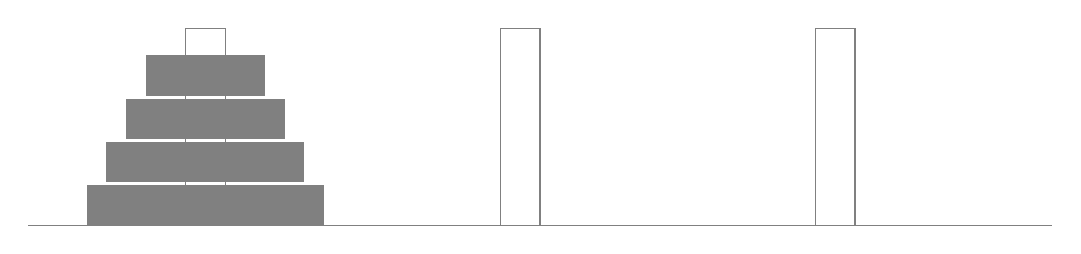
\begin{tikzpicture}[scale=0.5]
	\draw[gray, thin] (0,0) -- (26,0);
	\draw[gray, thin] (4,0) -- (4,5) -- (5,5) -- (5,0);
	\draw[gray, thin] (12,0) -- (12,5) -- (13,5) -- (13,0);
	\draw[gray, thin] (20,0) -- (20,5) -- (21,5) -- (21,0);

	\draw[gray, thin, fill=black!50] (1.5,0) -- (7.5,0) -- (7.5,1) -- (1.5,1) -- cycle;	
	\draw[gray, thin, fill=black!50] (2,1.1) -- (7,1.1) -- (7,2.1) -- (2,2.1) -- cycle;	
	\draw[gray, thin, fill=black!50] (2.5,2.2) -- (6.5,2.2) -- (6.5,3.2) -- (2.5,3.2) -- cycle;	
	\draw[gray, thin, fill=black!50] (3,3.3) -- (6,3.3) -- (6,4.3) -- (3,4.3) -- cycle;
\end{tikzpicture}

\end{center}

\end{problem}

\noindent
Tezę wykażemy indukcją po $n$. Zauważmy, że dla $n = 1$ teza jest oczywista -- wystarczy po prostu przełożyć dysk na trzecią igłę.

\vspace{10px}

\noindent
Załóżmy, że jesteśmy w stanie przełożyć $n - 1$ dysków z pierwszej igły na trzecią. Możemy oczywiście zauważyć, że jest to równoważne chociażby możliwości przełożenia ich z igły pierwszej na drugą.
Przełożenia $n$ dysków dokonujemy w następujący sposób:

\begin{enumerate}
	\item Przekładamy $n - 1$ dysków z góry pierwszej igły na drugą igłę. Zauważmy, że dysk o największym rozmiarze nie przeszkadza nam skorzystać z założenia indukcyjnego, gdyż nie uniemożliwi on wykonania żadnego ruchu.

	\item Dysk pozostawiony na pierwszej igle przekładamy na igłę ostatnią.

	\item Przekładamy $n - 1$ dysków z drugiej igły na trzecią. Analogicznie zauważamy, że obecność jednego dysku na trzeciej igle nie jest problemem.
\end{enumerate}

\begin{problem}{4}
	W przestrzeni danych jest $n \geqslant 3$ punktów, że żadne trzy z nich nie leżą na jednej prostej. Każde dwa z tych punktów połączono odcinkiem o kolorze zielonym lub czerwonym. Wykazać, że można wybrać tak jeden z tych kolorów, aby każde dwa z danych punktów były połączone odcinkiem lub łamaną tego koloru.
\end{problem}

\noindent
Dla $n = 3$ mamy trójkąt. Wybierając kolor, na który pomalowano co najmniej dwa odcinki, postulowana własność będzie spełniona.
\vspace{10px}

\noindent
Załóżmy, że dla teza zachodzi dla $n$ punktów. Rozpatrzmy zbiór $n + 1$ punktów. Wyróżnijmy pewien punkt $P$. Punktów poza $P$ jest dokładnie $n$, więc na mocy założenia istnieje kolor -- bez straty ogólności czerwony -- że pomiędzy każdymi dwoma punktami poza $P$ istnieje łamana tego koloru. 

\begin{minipage}{0.5\textwidth}
\begin{center}
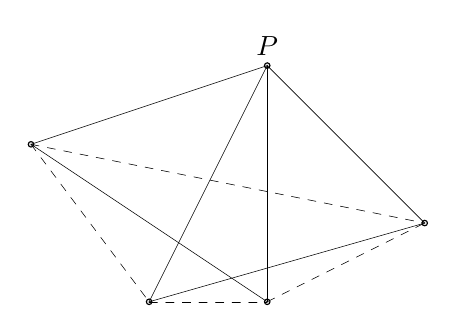
\begin{tikzpicture}
\tkzDefPoint(3,3){P}
\tkzDefPoint(0,2){v_1}
\tkzDefPoint(1.5,0){v_2}
\tkzDefPoint(3,0){v_3}
\tkzDefPoint(5,1){v_4}
\tkzDrawPoints(P, v_1,v_2,v_3,v_4)
\tkzDrawSegments[dashed](v_1,v_2 v_2,v_3 v_3,v_4 v_1,v_4)
\tkzDrawSegments(v_1,v_3 v_2,v_4)
\tkzDrawSegments(P,v_2 P,v_3 P,v_4 v_1,P)
\tkzLabelPoints[above](P)
\end{tikzpicture}\\

\end{center}
\end{minipage}
\begin{minipage}{0.5\textwidth}
\begin{center}
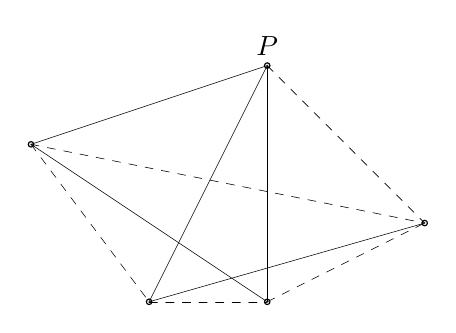
\begin{tikzpicture}
\tkzDefPoint(3,3){P}
\tkzDefPoint(0,2){v_1}
\tkzDefPoint(1.5,0){v_2}
\tkzDefPoint(3,0){v_3}
\tkzDefPoint(5,1){v_4}
\tkzDrawPoints(P, v_1,v_2,v_3,v_4)
\tkzDrawSegments[dashed](v_1,v_2 v_2,v_3 v_3,v_4 v_1,v_4 P,v_4)
\tkzDrawSegments(v_1,v_3 v_2,v_4)
\tkzDrawSegments(P,v_2 P,v_3  v_1,P)
\tkzLabelPoints[above](P)
\end{tikzpicture}\\
\end{center}
\end{minipage}
\begin{center}
Na rysunku zamiast kolorów użyto podziału na linię ciągłą i przerywaną.
\end{center}

Rozpatrzmy dwa przypadki:
\begin{enumerate}
	\item Punkt $P$ jest połączony czerwoną krawędzią z pewnym innym punktem $Q$. Wówczas, wybierając dowolny punkt $X$, na mocy założenia wiemy, że istnieje czerwona ścieżka między $X$ i $Q$. Dokładając do niej odcinek między $P$ i $Q$ otrzymujemy ścieżkę między $P$ oraz $X$.
	Wykazaliśmy, że istnieje ścieżka między punktem $P$ i każdym innym punktem. Łącząc to z faktem, że na mocy założenia indukcyjnego taka ścieżka istnieje między każdą inną parą punktów, otrzymujemy, że dla koloru czerwonego teza jest spełniona.
	\item Punkt $P$ jest połączony z każdym innym punktem niebieskim odcinkiem. Wówczas łatwo zauważyć, że pomiędzy każda parą punktów możemy przejść jednym albo dwoma niebieskimi odcinkami przechodzącymi przez punkt $P$.
\end{enumerate}

\begin{problem}{5}
Dany jest ciąg liczb rzeczywistych
\[
	a_0 \neq 0, 1,\quad a_1 = 1 - a_0,\quad a_{n + 1} = 1 - a_n(1 - a_n). 
\]
Wykazać, że dla wszystkich $n$ 
\[
	a_0a_1a_2...a_n\left(\frac{1}{a_0} + \frac{1}{a_1} + \frac{1}{a_2} + ... + \frac{1}{a_n}\right) = 1.
\]
\end{problem}

\noindent
Na początku wykażemy indukcyjnie, że dla każdego $n$ zachodzi równość
\[
	a_{n + 1} = 1 - a_0a_1a_2\cdot ... \cdot a_{n}.
\]
Równość dla $n = 0$ zachodzi na mocy założeń.
Załóżmy, że
\[
	a_{n} = 1 - a_0a_1a_2\cdot ... \cdot a_{n - 1}.
\]
Skoro $a_{n + 1} = 1 - a_n(1 - a_n)$, to otrzymujemy
\[
	a_{n + 1} = 1 - a_n(1 - a_n) = 1 - a_n \cdot a_0a_1a_2\cdot ... \cdot a_{n - 1} = 1 - a_0a_1a_2\cdot ... \cdot a_{n}.
\]
Więc na mocy zasady indukcji matematycznej postulowana równość zachodzi.
\vspace{10px}

\noindent
Teraz przejdziemy do udowodnienia tezy.
Dla $n = 1$ jest ona oczywista.
Załóżmy, że zachodzi równość
\[
	a_0a_1a_2...a_n\left(\frac{1}{a_0} + \frac{1}{a_1} + \frac{1}{a_2} + ... + \frac{1}{a_n}\right) = 1.
\]
Chcemy wykazać, że
\[
	a_0a_1a_2...a_na_{n+1}\left(\frac{1}{a_0} + \frac{1}{a_1} + \frac{1}{a_2} + ... + \frac{1}{a_n} + \frac{1}{a_{n + 1}}\right) = 1.
\]
Przekształcamy powyższą równość korzystając z założenia
\begin{multline*}
	a_0a_1a_2...a_na_{n+1}\left(\frac{1}{a_0} + \frac{1}{a_1} + \frac{1}{a_2} + \frac{1}{a_3} + ... + \frac{1}{a_n} + \frac{1}{a_{n + 1}}\right) = \\ = a_{n+1} \cdot a_0a_1a_2...a_n\left(\frac{1}{a_0} + \frac{1}{a_1} + \frac{1}{a_2} + ... + \frac{1}{a_n}\right) + a_0a_1a_2...a_n = \\ = a_{n + 1} + a_0a_1a_2...a_n = 1 - a_0a_1a_2...a_n + a_0a_1a_2...a_n = 1.
\end{multline*}

\begin{problem}{6}
	Wykazać, że planszę o wymiarach $2^n \times 2^n$ dla pewnego $n \geqslant 1$ z usuniętym jednym z rogów da się przykryć pewną liczbą $L$ klocków(takich jak na rysunku). Klocki można obracać.

	\begin{center}
		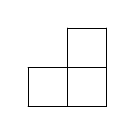
\begin{tikzpicture}[scale=0.5]
	    \tkzDefPoint(0,0){v_1}
	    \tkzDefPoint(2,0){v_2}
	    \tkzDefPoint(2,2){v_3}
	    \tkzDefPoint(1,2){v_4}
	    \tkzDefPoint(1,1){v_5}
	    \tkzDefPoint(0,1){v_6}
	    \tkzDefPoint(1,0){A}
	    \tkzDefPoint(2,1){B}

	    \tkzDrawSegments(v_1,v_2 v_2,v_3 v_3,v_4 v_4,v_5 v_5,v_6  v_6,v_1)
	    \tkzDrawSegments(v_5,A)
	    \tkzDrawSegments(v_5,B)
		\end{tikzpicture}
	\end{center}
\end{problem}

\noindent
Zauważmy, że plansza $2\times2$ z usuniętym rogiem jest w istocie L-klockiem, więc da się ją pokryć.

\begin{center}
	\begin{tikzpicture}[scale=0.3]
    \tkzDefPoint(0,0){A}
    \tkzDefPoint(0,10){B}
    \tkzDefPoint(10,10){C}
    \tkzDefPoint(10,0){D}
    \tkzDefPoint(9,0){P1}
    \tkzDefPoint(9,1){P2}
    \tkzDefPoint(10,1){P3}
    \tkzDrawSegments(A,B B,C C,D D,A)
    \tkzDrawSegments(P2,P1 P3,P2)


    \tkzDefPoint(5,0){G1}
    \tkzDefPoint(5,10){G2}
    \tkzDefPoint(0,5){G3}
    \tkzDefPoint(10,5){G4}
    \tkzDrawSegments(G1,G2 G3,G4)

    \tkzDefPoint(4,4){T1}
    \tkzDefPoint(4,6){T2}
    \tkzDefPoint(6,6){T3}
    \tkzDefPoint(6,5){T4}
    \tkzDefPoint(5,4){T5}
    \tkzDrawSegments(T1,T2 T2,T3 T3,T4 T1,T5) 
	\end{tikzpicture}\\
\end{center}

\noindent
Załóżmy, że dla planszy $2^{n - 1} \times 2^{n - 1}$ istnieje szukane pokrycie. Pokrycie dla planszy $2^{n} \times 2^{n}$ konstruujemy następująco. Dzielimy planszę dwiema prostymi na trzy jednakowe części i czwartą taką samą, tylko bez rogu. Kładziemy jeden klocek na środku, tak jak na rysunku. Wówczas plansza jest podzielona na cztery jednakowe puste części, które na mocy założenia indukcyjnego można pokryć.

\begin{problem}{7}
Niech $n$ będzie nieparzystą liczbą naturalną, a liczby $x_1,\; x_2,\; ...,\; x_n$ będa parami różne. Dla każdych dwóch liczb $x_i$ oraz $x_j$ zapisano na tablicy wartość bezwzględną ich różnicy. Wykazać, że można podzielić zapisane liczby na dwa zbiory o równej sumie.
\end{problem}
\noindent
Przez multizbiór rozumiemy zbiór w którym jeden element może występować kilka razy.
Załóżmy, że $x_1 \geqslant x_2 \geqslant ... \geqslant x_n$. 
\vspace{10px}

\noindent
Wykażemy tezę dla $n = 3$. Podział na zbiory $\{x_1 - x_2, x_2 - x_3\}$ oraz $\{x_1 - x_3\}$ spełnia warunki zadania.
\vspace{10px}

\noindent
Załóżmy, że teza zachodzi dla $2n + 1$, wykażemy ją dla $2n + 3$.
Rozpatrzmy szukany podział multizbioru różnic zbioru $\{x_1, x_2, ..., x_{2n + 1}\}$ na multizbiory $A$ i $B$ o równej sumie elementów.
Dorzucamy do multizbioru $A$ liczby
\[
	{x_{2k+3}-x_{2k+1}, \; x_{2k+3}-x_{2k},\; \cdots, \; x_{2k+3}-x_{k+2}} \quad \text{i} \quad {x_{2k+2}-x_{k+1},\; \cdots, \; x_{2k+2}-x_1},
\]
a do multizbioru $B$ liczby
\begin{gather*}
	x_{2k+3} - x_{2k+2} \quad \text{i} \quad x_{2k+2} - x_{2k+1},\; x_{2k+2} - x_{2k},\; \cdots,\; x_{2k+3} - x_{k+2}  \\ \text{oraz} \quad {x_{2k+3} - x_{k+1},\; \cdots, \; x_{2k+3}-x_1}.
\end{gather*}
Łatwo sprawdzić, że suma dorzuconych elementów jest równa. Stąd wynika, że otrzymane zbiory również mają równą sumę elementów, co jest równoważne tezie.
\newpage
\solutions{Równania funkcyjne}

\begin{problem}{1} 
	Znajdź wszystkie funkcje $\mathbb{R} \rightarrow \mathbb{R} $ spełniające dla wszystkich $x, y \in \mathbb{R} $ równanie
	\[
		 f(x)+f(y) = f(xy).
	\]
\end{problem}

\answer{Jedyną funkcją spełniającą warunki zadania jest $f(x) = 0$.}

\noindent
Podstawmy $y=0$: \[ f(x) + f(0) = f(0), \] czyli $f(x) =0$ dla każdego x. Łatwo sprawdzić, że ta funkcja spełnia warunki zadania. 

\vspace{10px}

\begin{problem}{2}
	Znajdź wszystkie funkcje $\mathbb{R} \rightarrow \mathbb{R} $ spełniające dla wszystkich $x, y \in \mathbb{R} $ równanie
	\[
		 f(x-f(y)) = 1 - x - y.
	\]
\end{problem}

\noindent
Podstawmy $x = f(y)$. Otrzymamy 
\begin{gather*}
	f(0) = 1 - f(y) - y, \\
	f(y) = - y + (1 - f(0)).
\end{gather*} 
Podstawmy $y = 0$ do powyższej zależności. Wówczas łatwo obliczyć, że $f(0)=\frac{1}{2}$. Czyli $f(x) = - x + \frac{1}{2} $. Ta funkcja istotnie spełnia warunki zadania, gdyż
\[
	f(x - f(y)) = f(y) - x + \frac{1}{2} = 1 - y - x .
\]

\begin{problem}{3}
	Znajdź wszystkie funkcje $\mathbb{R} \rightarrow \mathbb{R} $ spełniające dla wszystkich $x, y \in \mathbb{R} $ równanie 
	\[
		f(x^{2}y) = f(xy) + yf(f(x) + y).
	\]
\end{problem}

\answer{Funkcja $f(x) = x$ jest jedynym rozwiązaniem.}

\noindent
Podstawmy $x = 0$ i $y = -f(0)$. Otrzymamy $f(0)^{2}=0$, czyli $f(0)=0$. Podstawmy $x=0$: 
\[ 
	0 = yf(f(0) + y) = yf(y)
\] 
Dla niezerowego $y$ mamy $f(y) = 0$.
Sprawdzamy, że funkcja $f(x) = 0$ spełnia warunki zadania. Łącząc powyższe wnioski otrzymujemy, że jedyni funkcja $f(x)=0$ spełnia warunki zadania. 

\newpage

\begin{problem}{4}
	Znajdź wszystkie funkcje $\mathbb{R} \rightarrow \mathbb{R} $ spełniające dla wszystkich $x, y \in \mathbb{R} $ równanie 
	\[
		2f(x) + f(1 - x) = x^{2}.
	\] 
\end{problem}

\answer{Jedyną funkcją spełniającą warunki zadania jest $f(x) = \frac{2x^2 - (1-x)^2}{3}$.}

\noindent
Podstawmy $1-x$ za x. Otrzymamy 
\[ 
	2f(1 - x) + f(x) = 2(1 - x)^{2}.
\] 
Z równaniem z zadania tworzy to układ równań ze zmiennymi $f(x)$ i $f(1 - x)$. Wyliczamy $f(x) = \frac{2x^{2}-(1-x)^{2}} {3} $. Wystarczy teraz tylko sprawdzić, że ta funkcja spełnia warunki zadania. 

\vspace{5px}

\begin{problem}{5}
	Znajdź wszystkie funkcje $\mathbb{R} \rightarrow \mathbb{R} $ spełniające dla wszystkich $x, y \in \mathbb{R} $ równanie 
	\[
		f(x+y) = f(f(x)) + y + 1.
	\] 
\end{problem}

\answer{$f(x) = x - 1$ jest jedynym rozwiązaniem danego równania.}

\noindent
Podstawmy $x = 0$: 
\[
 f(y) = f(f(0)) + 1 + y, 
\] 
czyli $f(x) = x + a$ dla pewnego stałego a. Podstawmy tę funkcję do wyjściowego równania
\[
	x+y+a=x+2a+y+1.
\] 
Mamy $a = -1$. Łatwo sprawdzić, że funkcja $f(x) = x - 1$ spełnia warunki zadania. 

\vspace{5px}

\begin{problem}{6}
	Znajdź wszystkie funkcje różnowartościowe
	$\mathbb{R} \rightarrow \mathbb{R} $ spełniające dla wszystkich $x, y \in \mathbb{R} $ równość 
	\[
		f(f(x) + y) = f(x+y) + 1.
	\]
\end{problem}

\answer{Jedyną funkcją spełniającą warunki zadania jest $f(x) = x + 1$.}

\noindent
Podstawmy $y = -x$. Otrzymamy 
\[ 
	f(f(x) - x) = f(0) + 1.
\] 
Zauważmy, że prawa strona równości jest stała. Z różnowartościowości f wynika, że wartość $f(x) - x$ jest stała. Czyli $f(x) - x = a$ dla pewnego a. Wstawiamy $f(x) = x + a$ do wyjściowego równania 
\[
	x + y + 2a = x + y + a + 1,
\]
więc $a = 1$. Skąd $f(x) = x + 1 $ -- możemy sprawdzić, że ta funkcja spełnia warunki zadania.

\newpage

\begin{problem}{7}
	Znajdź wszystkie funkcje 
	$\mathbb{R} \rightarrow \mathbb{R} $ spełniające dla wszystkich $x, y \in \mathbb{R} $ nierówność 
	\[
		f(x^2+y) + f(y) \geqslant f(x^2) + f(x).
	\] 
\end{problem}

\noindent
Podstawmy $x = 0$
\[ 
	f(y) \geqslant f(0). 
\] 
Podstawmy $y = 0$ 
\[ 
	f(x^2) + f(0) \geqslant f(x^2) + f(x), 
\] 
czyli $f(0) \geqslant f(x) $. 
Łącząc oba wnioski otrzymuję 
\[ 
	f(0) \geqslant f(x) \geqslant f(0), 
\] 
czyli $f(x) = f(0)$. Innymi słowy $f$ jest funkcją stałą. Łatwo zauważyć, że taka funkcja spełnia warunki zadania. 

\vspace{5px}

\begin{problem}{8}
	Znajdź wszystkie funkcje $\mathbb{Z} \rightarrow \mathbb{Z} $ spełniające dla wszystkich $x \in \mathbb{Z} $ równanie
	\[
		 f(f(x)) =x+1.
	\] 
\end{problem}

\answer{Szukane funkcje nie istnieją.}

\noindent
Zauważmy, że zachodzą równości 
\begin{gather*} 
f(f(f(x))) = f(x + 1) \\
f(f(f(x))) = f(x) +1 
\end{gather*} 
Z tego otrzymujemy równość: 
\[
	f(x) =f(x-1)+1 
\] 
Skoro działamy w liczbach całkowitych to możemy wywnioskować, że
\[
	f(x) = f(x - 1) + 1 = f(x - 2) +  2 =  ... = x + f(0).
\] 
Podstawmy równość $f(x) = x + f(0)$ do 
$f(f(x)) = x + 1$:
\[
	x + 1 = f(f(x))= x + 2f(0), 
\]
czyli $f(0) = \frac{1}{2}$. Sprzeczność. Takie funkcje nie istnieją.

\vspace{5px} 

\begin{problem}{9}
	Znajdź wszystkie funkcje $\mathbb{R} \rightarrow \mathbb{R} $ spełniające dla wszystkich $x, y \in \mathbb{R} $ równanie 
	\[
		f(x) f(y) = f(x-y).
	\] 
\end{problem}

\answer{Daną zależność spełniają funkcje $f(x) = 1$ i $f(x) = 0$.}

\noindent
Podstawmy $x = y = 0$. Wtedy otrzymujemy 
\[
	f(0)^{2} = f(0) \implies f(0) \in \{0, 1\}.
\]
Podstawmy $x = y$
\[
	f(x)^{2} = f(0).
\] 
Jeśli $f(0)=0$, to $f(x) =0$. Łatwo sprawdzić, że funkcja zerowa spełnia warunki zadania.
Zobaczmy, co jeśli $x = y$ oraz $f(0) = 1$:
\[
	f(x)^{2} = f(0) = 1 
\] 
Czyli $f(x)$ jest równe $-1$ lub 1 dla każdego $x$.
Podstawmy $x=0$
\[
	f(y) =f(-y).
\] 
Zauważmy, że 
\[
	f(x - y) = f(x)f(y) = f(x)f(-y) = f(x+y). 
\] 
Weźmy 2 dowolne liczby a i b. Biorąc $x=\frac{a+b}{2}$ oraz 
$y=\frac{a-b}{2}$ otrzymamy
\[
	f(x+y) = f(x-y) \implies f(a) = f(b).
\] 
Skoro $a$ i $b$ były dowolne to $f$ jest funkcją stałą, czyli $f(x) = 1$. Łatwo sprawdzić, że ta funkcja również spełnia warunki zadania. Czyli tę zależność spełniają funkcje $f(x) = 1 $ i $f(x) = 0$. Sprawdzamy, że istotnie one działają.

\vspace{5px}

\begin{problem}{10}
	Udowodnij, że nie istnieje taka funkcja $f:\mathbb{R}\longrightarrow\mathbb{R}$, że dla dowolnych liczb rzeczywistych $x$, $y$ zachodzi równość:
	\[
		f(f(x) + 2f(y)) = x + y.
	\]
\end{problem}

\noindent
\underline{Lemat 1} Funkcja $f$ jest różnowartościowa

Załóżmy, że $f(a) = f(b)$. Podstawmy, $x=a$ oraz $x = b$
\[
	f(f(a) + 2f(y)) = a + y \quad \text{oraz} \quad f(f(b) + 2f(y)) = b + y.
\] 
Skoro $f(a)=f(b)$, to 
\[
	f(f(a) + 2f(y)) = f(f(b) + 2f(y)),
\] 
a więc $a + y = b + y$, czyli $a = b$. A więc $f$ istotnie jest różnowartościowa.
\vspace{10px}

\noindent
Zauważamy, że zachodzą równości
\[
	f(f(x) + 2f(y)) = x + y \quad \text{oraz} \quad f(f(y)+2f(x))=x+y.
\]
Czyli 
\[
	f(f(x) + 2f(y)) = f(f(y) + 2f(x)).
\] 
Skoro $f$ jest różnowartościowa, to 
\[
	f(x)+2f(y)=f(y)+2f(x),
\]
więc $f(x)=f(y)$ dla wszystkich liczb $x$, $y$. Czyli $f$ musiałaby być funkcją stałą, a to jest oczywista sprzeczność z danym równaniem.

\newpage
\solutions{Bijekcje i bajki kombinatoryczne}


\begin{problem}{1} 
	Dane są liczby całkowite $n$ i $k$. Wykaż, że
	\[
		\sum^{n}_{k=0} k \cdot {{n}\choose{k}} = n \cdot 2^{n - 1}.
	\]
\end{problem}

\vspace{5px}

\noindent
Spośród $n$ osób będziemy chcieli wybrać drużynę i mianować jednego jej członka kapitanem. Wykażemy, że wyrażenia po obu stronach równości są liczbą możliwości takiego wyboru.

Wybierając najpierw kapitana -- możemy go wybrać na $n$ sposobów -- a następnie dobierając mu zawodników -- których można wybrać na $2^{n - 1}$ sposobów, gdyż wybieramy dowolny podzbiór $n - 1$ osób -- otrzymamy $n \cdot 2^{n - 1}$ osób.

Przyjmijmy, że w drużynie wraz z kapitanem jest $k$ osób. Możliwości wyboru $k$ osób spośród $n$ jest ${n}\choose{k}$, a opcji wyboru kapitana spośród tych $k$ osób jest dokładnie $k$. Stąd też dla dowolnego $k$ liczba wariantów wynosi $k \cdot {{n}\choose{k}} $. Sumując po wszystkich możliwych $k$ otrzymujemy, że łączna liczba możliwości wynosi $\sum^{n}_{k=0} k \cdot {{n}\choose{k}}$.

\vspace{5px}

\begin{problem}{2}
	Wyznacz liczbę podzbiorów zbioru $\{1, 2, 3, ..., 10\}$, których suma wynosi co najmniej $27$.
\end{problem}

\vspace{5px}

\answer{Szukana liczba podzbiorów wynosi $2^9 = 512$.}

\noindent
Zauważmy, że suma wszystkich elementów tego zbioru wynosi $55$. Dla każdego podzbioru $A$ zdefiniujmy jego dopełnienie jako pozbiór $\{1, 2, 3, ..., 10\} - A$. Składa się on z wszystkich elementów nie występujących w $A$. Dla przykładu dopełnieniem zbioru $\{1, 2, 4, 7, 8, 9\}$ będzie zbiór $\{3, 5, 6, 10\}$.

Zauważmy, że suma elementów dowolnego podzbioru i jego dopełnienia wynosi $55$. Więc dokładnie jeden z tych zbiorów ma sumę elementów większą lub równą $27$. Podzielmy wszystkie rozpatrywane pozdbiory na pary zawierające dwa zbiory będące swoim dopełnieniem. Z powyższej obserwacji wynika, że dokładnie połowa podzbiorów -- po jednym z każdej pary -- będzie spełniać warunki zadania. Jest więc ich $\frac{1}{2} \cdot 2^{10} = 2^9 = 512$.


\newpage

\begin{problem}{3} 
	Udowodnić, że dla wszystkich dodatnich liczb całkowitych $n$, $k$ zachodzi równość
	\[
	    \sum^{n}_{k=0} {{n}\choose{k}}^2 = {{2n}\choose{n}}.
	\]
\end{problem}

\vspace{5px}

\noindent
Prawa strona równości jest równa liczbie sposobów wyboru $n$ spośród $2n$ osób.

Podzielmy te $2n$ osób na dwie grupy po $n$ osób. Załóżmy, że z pierwszej grupy wybieramy $k$ osób. Możemy tego dokonać na ${n}\choose{k}$ sposobów. Z drugiej grupy wybieramy $n - k$ osób -- mamy ${{n}\choose{n - k}} = {{n}\choose{k}}$ możliwości. Dla ustalonego $k$ możemy dokonać wyboru na ${{n}\choose{k}}^2$ sposobów. Sumując po wszystkich $k$ otrzymujemy lewą stronę równości.

\begin{problem}{4}
	Dana jest liczba pierwsza $p \geqslant 3$. Niech $A_k$ oznacza zbiór permutacji $(a_1, a_2, ..., a_p)$ zbioru $\{1, 2, 3,..., p\}$, dla których liczba
	\[
		a_1 + 2a_2 + 3a_3 + ... + pa_p - k
	\]
	jest podzielna przez $p$. Wykazać, że zbiory $A_1$, $A_2$ mają tyle samo elementów.
\end{problem}

\vspace{5px}

\noindent
Ideą poniższego rozwiązania jest fakt, że jak mamy pewną permutację z $A_1$, pomnożymy każdy jej z elementów przez 2, to otrzymamy permutację z $A_2$. Jako, że mnożąc liczbę większą od $\frac{1}{2}p$ przez $2$ wylecimi ze zbioru $\{1, 2, 3,..., p\}$ to zamiast mnożenia przez $2$ użyjemy funkcji danej wzorem
\[
	f(x) = 
	\begin{cases}
	2x \;\;\; \quad\quad\text{dla} \;\; x < \frac{1}{2}p\\
	2x - p \quad \text{dla} \;\; x > \frac{1}{2}p.
	\end{cases}
\]
Zauważmy, że $f(x) \equiv 2x \pmod{p}$.

W ten sposób przyporządkujemy każdemu elementowi ze zbioru $A_1$ dokładnie 1 element ze zbioru $A_2$. Czy może się jednak tak zdarzyć, że pewien element z $A_2$ zostanie w ten sposób przyporządkowany nie do jednego, a do innej liczby elementów z $A_1$? Wykażemy, że nie.

Mianowicie pokażemy, że z dowolnego elementu $A_2$ możemy odzyskać dokładnie jedną przyporządkowaną mu permutację z $A_1$. Zdefiniujmy ,,dzielenie przez $2$ modulo $p$'' wzorem
\[
	g(x) = 
	\begin{cases}
	\frac{1}{2}x \;\; \quad\quad\quad\text{dla x parzystych}\\
	\frac{1}{2}(x - p) \quad \text{dla x nieparzystych}.
	\end{cases}
\]
Mamy $2g(x) \equiv x \pmod{p}$.
Zauważmy, że jest to funkcja odwrotna do $f$ -- tj. $f(g(x)) = x$.

Zauważmy, że
\[
	(a_1, a_2, ..., a_p) \in A_2 \iff (g(a_1), g(a_2), ..., g(a_p)) \in A_1.
\] 
Pozostaje zauważyć, że to permutacja $(a_i)$ była przyporządkowana do permutacji~$(g(a_i))$. Jest tak, bo $f(g(a_i)) = a_i$. Stąd podane parowanie było poprawne, czyli istotnie zbiory $A_1$ i $A_2$ są równoliczne.

\remark{Kluczowym faktem w powyższym rozumowaniu było istnienie funkcji odwrotnej do funkcji $f$ zdefiniowanej dla każdego elementu zbioru $\{1, 2, ..., p\}$.} 

\vspace{5px}

\begin{problem}{5}
	Wykaż, że dla dowolnych dodatnich liczb całkowitych $n$, $k$ liczba	(kn)!
	jest podzielna przez liczbę $(n!)^k \cdot k!$.
\end{problem}

\vspace{5px}

\noindent
Rozpatrzmy liczbę podziałów $kn$ osób na $k$ grup po $n$ osób. Nie bierzemy pod uwagę żadnej kolejności grup, ani kolejności osób w grupie. 

Możemy ustawić $kn$ osób w kolejce na $(kn)!$ sposobów, a następnie pierwsze $n$ osób dać do jednej grupy, drugie $n$ osób do drugiej, itd. 

Każdą z $k$ grup możemy ustawić w kolejności na $n!$ sposobów. Te grupy możemy ustawić w kolejności na $k!$ sposobów. W ten sposób z jednego podziału na grupu możemy uzyskać dokładnie $(n!)^k \cdot k!$ kolejek. 

Więc liczba podziałów na grupy wynosi $\frac{(kn)!}{(n!)^k \cdot k!}$. Skoro jest ona całkowita, to musi zachodzić rozpatrywana podzielność.

\vspace{5px}



\begin{problem}{6}
	Dana jest liczba całkowita $n$. Niech $T_n$ oznacza liczbę takich podzbiorów zbioru $\{1, 2, 3, ..., n\}$, że ich średnia arytmetyczna jest liczbą całkowitą. Wykazać, że liczba $T_n - n$ jest parzysta.
\end{problem}

\vspace{5px}

% Source : https://prase.cz/kalva/putnam/psoln/psol023.html

\noindent
Zauważmy, że zbiory, których średnia arytmetyczna jest liczbą całkowitą, zawierające więcej niż $1$ element da się podzielić na pary. Mianowicie zbiory $S$ i $S'$ o średniej arytmetycznej elementów równej $a$ będa w jednej parze jeśli jeden z tych zbiorów zawiera $a$, drugi nie zawiera, a poza tym mają te same elementy.

$T_n$ będzie takiej parzystości jak liczba niesparowanych zbiorów. Są to wszystkie zbiory jednoelementowe -- jest ich $n$.  Stąd $T_n - n$ jest liczba parzystą.

\vspace{5px}

\begin{problem}{7}
	Niech $n$, $k$, $r$ będą dodatnimi liczbami całkowitymi. Wykaż, że
	\[
		\sum^{r}_{k=0} {{n + k}\choose{k}} = {{n + r + 1}\choose{r}} .
	\]
\end{problem}

\vspace{5px}

\noindent
Wykażemy, że obie strony równości to liczba słów, które składają się z $n + 1$ liter $A$ oraz $r$ liter $B$. Z jednej strony możemy wybrać na $r$ sposobów pozycje liter $B$, a na pozostałych miejscach ustawić litery $A$. Stąd tych słów jest ${{n + r + 1}\choose{r}}$.

Przyjmijmy, że na miejscu $n + k + 1$ znajduje się ostatnia litera $A$. Na $n + k$ poprzednich miejsc znajdzie się $n$ liter $A$ i $k$ liter $B$. Możemy je więc ustawić na ${{n + k}\choose{k}}$ sposobów. Po ostatniej literze $A$ będą same litery $B$, więc nie mamy wyboru. Stąd dla ustalonego $k$ jest ${{n + k}\choose{k}}$ sposobów. Sumując po wszystkich możliwych $k$ otrzymujemy lewą stronę równości.



\newpage
\solutions{Równania funkcyjne}

\begin{problem}{1} 
	Znajdź wszystkie funkcje $\mathbb{R} \rightarrow \mathbb{R} $ spełniające dla wszystkich $x, y \in \mathbb{R} $ równanie
	\[
		 f(x)+f(y) = f(xy).
	\]
\end{problem}

\answer{Jedyną funkcją spełniającą warunki zadania jest $f(x) = 0$.}

\noindent
Podstawmy $y=0$: \[ f(x) + f(0) = f(0), \] czyli $f(x) =0$ dla każdego x. Łatwo sprawdzić, że ta funkcja spełnia warunki zadania. 

\vspace{10px}

\begin{problem}{2}
	Znajdź wszystkie funkcje $\mathbb{R} \rightarrow \mathbb{R} $ spełniające dla wszystkich $x, y \in \mathbb{R} $ równanie
	\[
		 f(x-f(y)) = 1 - x - y.
	\]
\end{problem}

\noindent
Podstawmy $x = f(y)$. Otrzymamy 
\begin{gather*}
	f(0) = 1 - f(y) - y, \\
	f(y) = - y + (1 - f(0)).
\end{gather*} 
Podstawmy $y = 0$ do powyższej zależności. Wówczas łatwo obliczyć, że $f(0)=\frac{1}{2}$. Czyli $f(x) = - x + \frac{1}{2} $. Ta funkcja istotnie spełnia warunki zadania, gdyż
\[
	f(x - f(y)) = f(y) - x + \frac{1}{2} = 1 - y - x .
\]

\begin{problem}{3}
	Znajdź wszystkie funkcje $\mathbb{R} \rightarrow \mathbb{R} $ spełniające dla wszystkich $x, y \in \mathbb{R} $ równanie 
	\[
		f(x^{2}y) = f(xy) + yf(f(x) + y).
	\]
\end{problem}

\answer{Funkcja $f(x) = x$ jest jedynym rozwiązaniem.}

\noindent
Podstawmy $x = 0$ i $y = -f(0)$. Otrzymamy $f(0)^{2}=0$, czyli $f(0)=0$. Podstawmy $x=0$: 
\[ 
	0 = yf(f(0) + y) = yf(y)
\] 
Dla niezerowego $y$ mamy $f(y) = 0$.
Sprawdzamy, że funkcja $f(x) = 0$ spełnia warunki zadania. Łącząc powyższe wnioski otrzymujemy, że jedyni funkcja $f(x)=0$ spełnia warunki zadania. 

\newpage

\begin{problem}{4}
	Znajdź wszystkie funkcje $\mathbb{R} \rightarrow \mathbb{R} $ spełniające dla wszystkich $x, y \in \mathbb{R} $ równanie 
	\[
		2f(x) + f(1 - x) = x^{2}.
	\] 
\end{problem}

\answer{Jedyną funkcją spełniającą warunki zadania jest $f(x) = \frac{2x^2 - (1-x)^2}{3}$.}

\noindent
Podstawmy $1-x$ za x. Otrzymamy 
\[ 
	2f(1 - x) + f(x) = 2(1 - x)^{2}.
\] 
Z równaniem z zadania tworzy to układ równań ze zmiennymi $f(x)$ i $f(1 - x)$. Wyliczamy $f(x) = \frac{2x^{2}-(1-x)^{2}} {3} $. Wystarczy teraz tylko sprawdzić, że ta funkcja spełnia warunki zadania. 

\vspace{5px}

\begin{problem}{5}
	Znajdź wszystkie funkcje $\mathbb{R} \rightarrow \mathbb{R} $ spełniające dla wszystkich $x, y \in \mathbb{R} $ równanie 
	\[
		f(x+y) = f(f(x)) + y + 1.
	\] 
\end{problem}

\answer{$f(x) = x - 1$ jest jedynym rozwiązaniem danego równania.}

\noindent
Podstawmy $x = 0$: 
\[
 f(y) = f(f(0)) + 1 + y, 
\] 
czyli $f(x) = x + a$ dla pewnego stałego a. Podstawmy tę funkcję do wyjściowego równania
\[
	x+y+a=x+2a+y+1.
\] 
Mamy $a = -1$. Łatwo sprawdzić, że funkcja $f(x) = x - 1$ spełnia warunki zadania. 

\vspace{5px}

\begin{problem}{6}
	Znajdź wszystkie funkcje różnowartościowe
	$\mathbb{R} \rightarrow \mathbb{R} $ spełniające dla wszystkich $x, y \in \mathbb{R} $ równość 
	\[
		f(f(x) + y) = f(x+y) + 1.
	\]
\end{problem}

\answer{Jedyną funkcją spełniającą warunki zadania jest $f(x) = x + 1$.}

\noindent
Podstawmy $y = -x$. Otrzymamy 
\[ 
	f(f(x) - x) = f(0) + 1.
\] 
Zauważmy, że prawa strona równości jest stała. Z różnowartościowości f wynika, że wartość $f(x) - x$ jest stała. Czyli $f(x) - x = a$ dla pewnego a. Wstawiamy $f(x) = x + a$ do wyjściowego równania 
\[
	x + y + 2a = x + y + a + 1,
\]
więc $a = 1$. Skąd $f(x) = x + 1 $ -- możemy sprawdzić, że ta funkcja spełnia warunki zadania.

\newpage

\begin{problem}{7}
	Znajdź wszystkie funkcje 
	$\mathbb{R} \rightarrow \mathbb{R} $ spełniające dla wszystkich $x, y \in \mathbb{R} $ nierówność 
	\[
		f(x^2+y) + f(y) \geqslant f(x^2) + f(x).
	\] 
\end{problem}

\noindent
Podstawmy $x = 0$
\[ 
	f(y) \geqslant f(0). 
\] 
Podstawmy $y = 0$ 
\[ 
	f(x^2) + f(0) \geqslant f(x^2) + f(x), 
\] 
czyli $f(0) \geqslant f(x) $. 
Łącząc oba wnioski otrzymuję 
\[ 
	f(0) \geqslant f(x) \geqslant f(0), 
\] 
czyli $f(x) = f(0)$. Innymi słowy $f$ jest funkcją stałą. Łatwo zauważyć, że taka funkcja spełnia warunki zadania. 

\vspace{5px}

\begin{problem}{8}
	Znajdź wszystkie funkcje $\mathbb{Z} \rightarrow \mathbb{Z} $ spełniające dla wszystkich $x \in \mathbb{Z} $ równanie
	\[
		 f(f(x)) =x+1.
	\] 
\end{problem}

\answer{Szukane funkcje nie istnieją.}

\noindent
Zauważmy, że zachodzą równości 
\begin{gather*} 
f(f(f(x))) = f(x + 1) \\
f(f(f(x))) = f(x) +1 
\end{gather*} 
Z tego otrzymujemy równość: 
\[
	f(x) =f(x-1)+1 
\] 
Skoro działamy w liczbach całkowitych to możemy wywnioskować, że
\[
	f(x) = f(x - 1) + 1 = f(x - 2) +  2 =  ... = x + f(0).
\] 
Podstawmy równość $f(x) = x + f(0)$ do 
$f(f(x)) = x + 1$:
\[
	x + 1 = f(f(x))= x + 2f(0), 
\]
czyli $f(0) = \frac{1}{2}$. Sprzeczność. Takie funkcje nie istnieją.

\vspace{5px} 

\begin{problem}{9}
	Znajdź wszystkie funkcje $\mathbb{R} \rightarrow \mathbb{R} $ spełniające dla wszystkich $x, y \in \mathbb{R} $ równanie 
	\[
		f(x) f(y) = f(x-y).
	\] 
\end{problem}

\answer{Daną zależność spełniają funkcje $f(x) = 1$ i $f(x) = 0$.}

\noindent
Podstawmy $x = y = 0$. Wtedy otrzymujemy 
\[
	f(0)^{2} = f(0) \implies f(0) \in \{0, 1\}.
\]
Podstawmy $x = y$
\[
	f(x)^{2} = f(0).
\] 
Jeśli $f(0)=0$, to $f(x) =0$. Łatwo sprawdzić, że funkcja zerowa spełnia warunki zadania.
Zobaczmy, co jeśli $x = y$ oraz $f(0) = 1$:
\[
	f(x)^{2} = f(0) = 1 
\] 
Czyli $f(x)$ jest równe $-1$ lub 1 dla każdego $x$.
Podstawmy $x=0$
\[
	f(y) =f(-y).
\] 
Zauważmy, że 
\[
	f(x - y) = f(x)f(y) = f(x)f(-y) = f(x+y). 
\] 
Weźmy 2 dowolne liczby a i b. Biorąc $x=\frac{a+b}{2}$ oraz 
$y=\frac{a-b}{2}$ otrzymamy
\[
	f(x+y) = f(x-y) \implies f(a) = f(b).
\] 
Skoro $a$ i $b$ były dowolne to $f$ jest funkcją stałą, czyli $f(x) = 1$. Łatwo sprawdzić, że ta funkcja również spełnia warunki zadania. Czyli tę zależność spełniają funkcje $f(x) = 1 $ i $f(x) = 0$. Sprawdzamy, że istotnie one działają.

\vspace{5px}

\begin{problem}{10}
	Udowodnij, że nie istnieje taka funkcja $f:\mathbb{R}\longrightarrow\mathbb{R}$, że dla dowolnych liczb rzeczywistych $x$, $y$ zachodzi równość:
	\[
		f(f(x) + 2f(y)) = x + y.
	\]
\end{problem}

\noindent
\underline{Lemat 1} Funkcja $f$ jest różnowartościowa

Załóżmy, że $f(a) = f(b)$. Podstawmy, $x=a$ oraz $x = b$
\[
	f(f(a) + 2f(y)) = a + y \quad \text{oraz} \quad f(f(b) + 2f(y)) = b + y.
\] 
Skoro $f(a)=f(b)$, to 
\[
	f(f(a) + 2f(y)) = f(f(b) + 2f(y)),
\] 
a więc $a + y = b + y$, czyli $a = b$. A więc $f$ istotnie jest różnowartościowa.
\vspace{10px}

\noindent
Zauważamy, że zachodzą równości
\[
	f(f(x) + 2f(y)) = x + y \quad \text{oraz} \quad f(f(y)+2f(x))=x+y.
\]
Czyli 
\[
	f(f(x) + 2f(y)) = f(f(y) + 2f(x)).
\] 
Skoro $f$ jest różnowartościowa, to 
\[
	f(x)+2f(y)=f(y)+2f(x),
\]
więc $f(x)=f(y)$ dla wszystkich liczb $x$, $y$. Czyli $f$ musiałaby być funkcją stałą, a to jest oczywista sprzeczność z danym równaniem.

\newpage
\solutions{Nierówności między średnimi}

\begin{problem}{1} 
	Wykazać, że dla dowolnej liczby rzeczywistej $x$ zachodzi
	\[
		x^2 + \frac{1}{x} \geqslant \frac{3}{2}\sqrt[3]{2}.
	\]
\end{problem}

\vspace{5px}

\noindent
Korzystając z nierówności między średnią arytemetyczną i geometryczną dla liczb $x^2, \frac{x}{2}, \frac{x}{2}$ otrzymujemy
\[
	\frac{x^2 + \frac{1}{x}}{3} = \frac{x^2 + \frac{x}{2} + \frac{x}{2}}{3} \geqslant \sqrt[3]{x^2 \cdot \frac{x}{2} \cdot \frac{x}{2}} = \sqrt[3]{\frac{1}{4}},
\]
z czego wprost wynika teza.

\vspace{5px}

%Source: well-known
\begin{problem}{2} 
	Dane są takie dodatnie liczby rzeczywiste $a_1, \;a_2,\; a_3,\; ...,\; a_n$, że $a_1a_2a_3...a_n = 1$. Wykazać, że
	\[
		(a_1 + a_2)(a_2 + a_3)\cdot ... \cdot (a_{n-1} + a_n)(a_n + a_1) \geqslant 2^n.
	\]
\end{problem}

\vspace{5px}

\noindent
Korzystając z nierówności miedzy średnią arytmetyczną a geometryczną mamy
\[
	a_i + a_{i + 1} \geqslant 2\sqrt{a_ia_{i + 1}}.
\]
Robiąc tak dla każdego nawiasu otrzymujemy, że
\begin{multline*}
	(a_1 + a_2)(a_2 + a_3)\cdot ... \cdot (a_{n-1} + a_n)(a_n + a_1) \geqslant \\
	\geqslant 2\sqrt{a_1a_{2}} \cdot 2\sqrt{a_2a_{3}} \cdot ... \cdot 2\sqrt{a_{n-1}a_{n}}\cdot 2\sqrt{a_na_{1}}  = \\
	= 2^n a_1a_2\cdot ... \cdot a_n = 2^n.
\end{multline*}

%Source: well-known
\begin{problem}{3} 
	Udowodnić, że dla dowolnych dodatnich liczb rzeczywistych zachodzi nierówność
	\[
		\frac{a}{b + c} + \frac{b}{a + c} + \frac{c}{a + b} \geqslant \frac{3}{2}.
	\]
\end{problem}

\vspace{5px}

\noindent
Przekształcamy tezę równoważnie dodając $3$ do obu stron
\begin{align*}
	\frac{a}{b + c} + 1 + \frac{b}{a + c} + 1 + \frac{c}{a + b} + 1 &\geqslant \frac{9}{2}, \\
	\frac{a + b + c}{b + c} + \frac{a + b + c}{a + c} + \frac{a + b + c}{a + b} &\geqslant \frac{9}{2}, \\
	\left(a + b + c\right)\left(\frac{1}{b + c} + \frac{1}{a + c} + \frac{1}{a + b}\right) &\geqslant \frac{9}{2}.
\end{align*}

\noindent
Zauważmy, że z nierówności miedzy średnią arytmetyczną i harmoniczną wynika
\[
	\frac{\frac{1}{b + c} + \frac{1}{a + c} + \frac{1}{a + b}}{3} \geqslant \frac{9}{(b + c) + (a + c) + (a + b)} = \frac{9}{2(a + b + c)},
\]
co jest równoważne nierówności, którą chcieliśmy wykazać.

\vspace{5px}

%Source: well-known
\begin{problem}{4} 
	Dane są takie dodatnie liczby rzeczywiste $a$, $b$, $c$, że $abc = 1$. Wykazać, że
	\[
		a^2 + b^2 + c^2 \geqslant a + b + c.
	\]
\end{problem}

\vspace{5px}

\noindent
Zauważmy, że zachodzą nierówności
\[
	(a - 1)^2 + (b - 1)^2 + (c - 1)^2 \geqslant 0,
\]
\[
	a^2 + b^2 + c^2 + 3 \geqslant 2a + 2b + 2c.
\]
Z nierówności między średnią arytmetyczną i geometryczną mamy
\[
	\frac{a + b + c}{3} \geqslant \sqrt[3]{abc} = 1,
\]
\[
	a + b + c \geqslant 3.
\]

\noindent
Dodając dwie otrzymane nierówności stronami udowadniamy tezę.

\vspace{5px}

%Source: https://om.mimuw.edu.pl/static/app_main/camps/oboz2015.pdf Problem 33
\begin{problem}{5} 
	Udowodnić, że dla dowolnych liczb rzeczywistych $a$, $b$, $c$ zachodzi nierówność
	\[
		\frac{a^2}{a + b} + \frac{b^2}{b + c} \geqslant \frac{3a + 2b - c}{4}. 
	\]
\end{problem}

\vspace{5px}

\noindent
Zauważmy, że z nierówności między średnią arymtetyczną i geometryczną dla liczb $\frac{a^2}{a + b}$ oraz $\frac{a + b}{4}$ otrzymujemy
\[
	\frac{a^2}{a + b} + \frac{a + b}{4} \geqslant a.
\]
Analogicznie mamy
\[
	\frac{a^2}{a + b} + \frac{b + c}{4} \geqslant b.
\]
Dodając te dwie równości stronami otrzymujemy
\[
	\frac{a^2}{a + b} + \frac{a^2}{a + b} + \frac{a + b}{4} + \frac{b + c}{4} \geqslant a + b,
\]
\[
	\frac{a^2}{a + b} + \frac{b^2}{b + c} \geqslant \frac{3a + 2b - c}{4},
\]
co było do wykazania.

\newpage
\solutions{Konstrukcje}

\begin{problem}{1} 
	Wykazać, że można pokolorować $40$ pól na nieskończonej szachownicy, tak, aby nie istniał prostokąt utworzony z pól tej szachownicy zawierający dokładnie $20$ pokolorowanych pól.
\end{problem}

\noindent
Rozpatrzmy kolorowanie takie jak na rysunku - pola, w które wpisano literę są pomalowane.

\begin{center}
    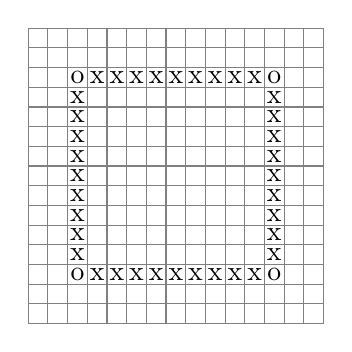
\begin{tikzpicture}[x=1cm, scale=0.25]
    \foreach \y in {-1,0,...,12}{
        \foreach \x in {-1,0,...,12}{
            \draw[black!50] (\x,\y) rectangle (1+\x,1+\y) rectangle (2+\x,2+\y);}}

    \draw[black!50] (-1,-1)--(14,-1)--(14,14)--(-1,14)--cycle;
    \node at (1.5,1.5) {o};
    \node at (2.5,1.5) {x};
    \node at (3.5,1.5) {x};
    \node at (4.5,1.5) {x};
    \node at (5.5,1.5) {x};
    \node at (6.5,1.5) {x};
    \node at (7.5,1.5) {x};
    \node at (8.5,1.5) {x};
    \node at (9.5,1.5) {x};
    \node at (10.5,1.5) {x};
    \node at (11.5,1.5) {o};

    \node at (1.5,11.5) {o};
    \node at (2.5,11.5) {x};
    \node at (3.5,11.5) {x};
    \node at (4.5,11.5) {x};
    \node at (5.5,11.5) {x};
    \node at (6.5,11.5) {x};
    \node at (7.5,11.5) {x};
    \node at (8.5,11.5) {x};
    \node at (9.5,11.5) {x};
    \node at (10.5,11.5) {x};
    \node at (11.5,11.5) {o};

    \node at (11.5,2.5) {x};
    \node at (11.5,3.5) {x};
    \node at (11.5,4.5) {x};
    \node at (11.5,5.5) {x};
    \node at (11.5,6.5) {x};
    \node at (11.5,7.5) {x};
    \node at (11.5,8.5) {x};
    \node at (11.5,9.5) {x};
    \node at (11.5,10.5) {x};

    \node at (1.5,2.5) {x};
    \node at (1.5,3.5) {x};
    \node at (1.5,4.5) {x};
    \node at (1.5,5.5) {x};
    \node at (1.5,6.5) {x};
    \node at (1.5,7.5) {x};
    \node at (1.5,8.5) {x};
    \node at (1.5,9.5) {x};
    \node at (1.5,10.5) {x};

    \end{tikzpicture}
\end{center}

\noindent
Zauważmy, że jeśli pewien prostokąt nie przykrywa żadnego pola z literą o, to może zawierać co najwyżej $18$ pokolorowanych pól. Jeśli zawiera tylko jedną, to może zawierać ich co najwyżej $19$. Jeśli zaś zawiera on w całości pewną ,,krawędź'' pokolorowanego prostokąta, to albo zawiera nieparzystą liczbę pól, albo zawiera je wszystkie. Więc szukany prostokąt nie istnieje.

\vspace{10px}

\begin{problem}{2} 
	Udowodnij, że punkty płaszczyzny można tak pokolorować dziewięcioma kolorami, aby żadne dwa punkty odległe o 1 nie były tego samego koloru.
\end{problem}

\noindent
Podzielmy płaszczyznę na kratkę, tak że przekątna każdej kratki ma długość $1$. Kolorujemy wszystkie punkty wewnątrz kratki, jej dolną krawędź bez prawego wierzchołka i jej lewą krawędź bez górnego wierzchołka na kolor przypisany według sposobu zademonstrowanego na lewym rysunku. 

\begin{center}
    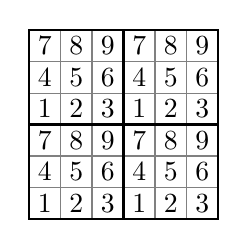
\begin{tikzpicture}[x=1cm, scale=0.4]
    \foreach \y in {0,...,4}{
        \foreach \x in {0,...,4}{
            \draw[black!50] (\x,\y) rectangle (1+\x,1+\y) rectangle (2+\x,2+\y);}}

    \draw[black!50] (0,0)--(6,0)--(6,6)--(0,6)--cycle;
    \draw[line width=1] (0,0)--(3,0)--(3,3)--(0,3)--cycle;
    \draw[line width=1] (0,3)--(3,3)--(3,6)--(0,6)--cycle;
    \draw[line width=1] (3,0)--(6,0)--(6,3)--(3,3)--cycle;
    \draw[line width=1] (3,3)--(6,3)--(6,6)--(3,6)--cycle;
    \node at (0.5,0.5) {1};
    \node at (1.5,0.5) {2};
    \node at (2.5,0.5) {3};
    \node at (3.5,0.5) {1};
    \node at (4.5,0.5) {2};
    \node at (5.5,0.5) {3};


    \node at (0.5,1.5) {4};
    \node at (1.5,1.5) {5};
    \node at (2.5,1.5) {6};
    \node at (3.5,1.5) {4};
    \node at (4.5,1.5) {5};
    \node at (5.5,1.5) {6};



    \node at (0.5,2.5) {7};
    \node at (1.5,2.5) {8};
    \node at (2.5,2.5) {9};
    \node at (3.5,2.5) {7};
    \node at (4.5,2.5) {8};
    \node at (5.5,2.5) {9};

    \node at (0.5,3.5) {1};
    \node at (1.5,3.5) {2};
    \node at (2.5,3.5) {3};
    \node at (3.5,3.5) {1};
    \node at (4.5,3.5) {2};
    \node at (5.5,3.5) {3};


    \node at (0.5,4.5) {4};
    \node at (1.5,4.5) {5};
    \node at (2.5,4.5) {6};
    \node at (3.5,4.5) {4};
    \node at (4.5,4.5) {5};
    \node at (5.5,4.5) {6};



    \node at (0.5,5.5) {7};
    \node at (1.5,5.5) {8};
    \node at (2.5,5.5) {9};
    \node at (3.5,5.5) {7};
    \node at (4.5,5.5) {8};
    \node at (5.5,5.5) {9};

    \end{tikzpicture}
    \hspace{30px}
    \begin{tikzpicture}[x=1cm, scale=0.4]
    \draw[line width=1] (0,0)--(4,0);
    \draw[line width=1] (0,0)--(0,4);
    \node at (0,0)[circle,fill,inner sep=1.5pt]{};
    %\node at (0,4)[circle,fill=white,draw,outer sep=0pt,inner sep=1.5pt]{};
    %\node at (4,0)[circle,fill=white,draw,outer sep=0pt,inner sep=1.5pt]{};
    \fill[pattern=north west lines] (0,0) rectangle (4,4);
    \end{tikzpicture}
\end{center}

\noindent
Łatwo zauważyć, że takie kolorowanie spełnia warunki zadania.

\begin{problem}{3}
	Wykazać, że każdy trójkąt można podzielić na $3000$ czworokątów wypukłych, tak, aby każdy z nich dało się wpisać w okrąg oraz opisać na okręgu.
\end{problem}

\noindent
Na początku wykażemy, że każdy trójkąt można podzielić na $3$ takie czworokąty. Rozpatrzmy dowolny trójkąt $ABC$. Niech $I$ to będzie środek okręgu weń wpisanego, a punkty $D$, $E$ i $F$ to będą rzuty $I$ odpowiednio na boki $BC$, $CA$ i $AB$. Zauważmy, że $IE = IF$(promienie okręgu) oraz $AF = AE$(odcinki styczne). Stąd $AF + IE = AE + IF$, czyli czworokąt $AFIE$ da się opisać na okręgu. Mamy też, że kąty $\an AFI$ i $\an AEI$ są proste, czyli czworokąt $AFIE$ da się wpisać w okrąg. Analogicznie rozumujemy dla czworokątów $BDIF$ oraz $CEID$.

\begin{center}
	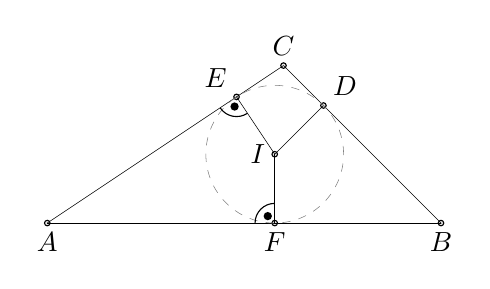
\begin{tikzpicture}
		\tkzDefPoint(0,0){A}
		\tkzDefPoint(5,0){B}
		\tkzDefPoint(3,2){C}

		\tkzDefTriangleCenter[in](A,B,C)\tkzGetPoint{I}
		\tkzDefPointsBy[projection=onto B--C](I){D}
		\tkzDefPointsBy[projection=onto C--A](I){E}
		\tkzDefPointsBy[projection=onto A--B](I){F}


		\tkzDrawPoints(A,B,C, I, D,E,F)
		\tkzDrawSegments(A,B B,C C,A I,D I,E I,F)
		\tkzDrawCircle[dashed](I,F)
		\tkzLabelPoints[below](A,B, F)
		\tkzLabelPoints[above](C)
		\tkzLabelPoints[left](I)
		\tkzLabelPoints[above left](E)
		\tkzLabelPoints[above right](D)
		\tkzMarkRightAngle[german](I,F,A)
		\tkzMarkRightAngle[german](A,E,I)
	\end{tikzpicture}
	\hspace{10px}
	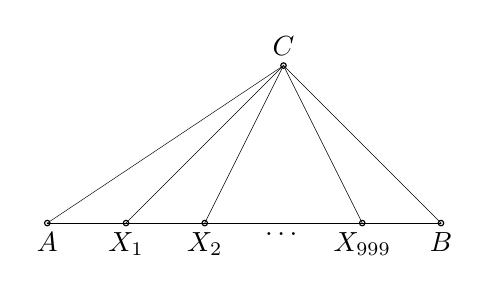
\begin{tikzpicture}
		\tkzDefPoint(0,0){A}
		\tkzDefPoint(5,0){B}
		\tkzDefPoint(3,2){C}
		\tkzDefPoint(1,0){X_1}
		\tkzDefPoint(2,0){X_2}
		\tkzDefPoint(4,0){X_{999}}
		\tkzDefPoint(3,0){T}

		\tkzDefTriangleCenter[in](A,B,C)\tkzGetPoint{I}
		\tkzDefPointsBy[projection=onto B--C](I){D}
		\tkzDefPointsBy[projection=onto C--A](I){E}
		\tkzDefPointsBy[projection=onto A--B](I){F}


		\tkzDrawPoints(A,B,C, X_1, X_2, X_{999})
		\tkzDrawSegments(C,X_1 C,X_2 C,X_{999})
		\tkzDrawSegments(A,B B,C C,A)
		\tkzLabelPoints[below](A,B,X_1, X_2, X_{999})
		\tkzLabelPoints[above](C)
		\tkzLabelPoint[below](T){$\dots$}
	\end{tikzpicture}
\end{center}

\noindent
Wystarczy więc podzielić wyjściowy trójkąt na $1000$ trójkątów jak na rysunku $1$, a następnie każdy z tych trójkątów podzielić na $3$ szukane czworokąty.

\vspace{10px}

\begin{problem}{4} 
	Wykazać, że można pokolorować każdą dodatnią liczbę całkowitą na jeden z $1000$ kolorów, tak aby
	\begin{itemize}
		\item każdy z kolorów był użyty nieskończenie wiele razy;
		\item dla dowolnych takich liczb całkowitych $a$, $b$, $c$, że $ab = c$, pewne dwie spośród nich sa jednakowego koloru.
	\end{itemize} 
\end{problem}

\vspace{5px}

\noindent
Przyjmijmy $p_1 = 2,\; p_2 = 3, \; ...$ jako kolejne liczby pierwsze. Liczbę $1$ kolorujemy dowolnym kolorem. Niech $p_i$ to będzie najmniejszy dzielnik pierwszy pewnej liczby $n$. Wówczas jeśli $i \leqslant 1000$ kolorujemy $n$ kolorem o numerze $i$. W przeciwnym wypadku kolorujemy go kolorem o numerze $1000$.

\vspace{5px}

\noindent
Wykażemy, że podane kolorowanie spełnia warunki zadania. Łatwo zauważyć, że każdy z kolorów będzie użyty nieskończenie wiele razy. Załóżmy więc, że $ab = c$. Jeśli jedna z liczb $a$, $b$ jest równa jeden, to pozostałe są równe, więc w szczególności są tego samego koloru. Niech $p$ będzie najmniejszym dzielnikiem liczby $abc$. Wówczas, skoro $ab = c$ liczba~$p$ musi dzielić co najmniej dwie spośród $a$, $b$, $c$. Z minimalności $p$ mamy, że wyznaczy ona jednakowy kolor obu tym liczbom.

\vspace{10px}

\begin{problem}{5}
	Łódka może zabrać w rejs po jeziorze dokładnie 7 osób. Udowodnij. że można tak zaplanować rejsy 49-osobowej wycieczki, aby każdych dwóch uczestników płynęło ze sobą dokładnie raz.
\end{problem}

\noindent
Zinterpretujmy te $49$ osób jako planszę 7 na 7, gdzie każdemu polu przyporządkowana jest jedna osoba. Rozpatrzmy wszystkie kolorowania powstające w następujący sposób. Kolorujemy dowolna pola w najniższym i drugim najniższym wierszu. Załóżmy, że są to pola $a$-te i $a + k$-te(być może $k < 0$). Wówczas w trzeciej kolumnie pokolorujemy pole $a + 2k \pmod{7}$, w czwartej $a + 3k \pmod{7}$ itd. Przykładowe kolorowanie dla $a = 2$ i~$k = 2$ jest na rysunku.


\begin{center}
    \begin{tikzpicture}[x=1cm, scale=0.4]
    \foreach \y in {0,...,5}{
        \foreach \x in {0,...,5}{
            \draw[black!50] (\x,\y) rectangle (1+\x,1+\y) rectangle (2+\x,2+\y);}}

    \draw[black!50] (0,0)--(7,0)--(7,7)--(0,7)--cycle;
    
    \fill[pattern=north west lines] (1,0) rectangle (2,1);
    \fill[pattern=north west lines] (3,1) rectangle (4,2);
    \fill[pattern=north west lines] (5,2) rectangle (6,3);
    \fill[pattern=north west lines] (0,3) rectangle (1,4);
    \fill[pattern=north west lines] (2,4) rectangle (3,5);
    \fill[pattern=north west lines] (4,5) rectangle (5,6);
    \fill[pattern=north west lines] (6,6) rectangle (7,7);

    \end{tikzpicture}
\end{center}

\noindent
Rozpatrzmy wszystkie takie kolorowania i dla każdego weźmy osoby przyporządkowane pokolorowanym polom na rejs. Wykażemy, że dowolne dwa pola są jednocześnie pokolorowane w dokładnie jednym kolorowaniu. Przyjmijmy, że te dwa pola są oddalone o $y \neq 0$ wierszy w pionie i $x$ kolumn w poziomie. Zauważmy, że wówczas musi zajść ${x \equiv yk \pmod{7}}$, co jest prawdą dla dokładnie jednego $k$. Skoro $k$ jest jednoznacznie wyznaczone i znamy położenie jednego pola z kolorowania, to możemy odtworzyć położenie wszystkich. Skoro z dwóch pól możemy jednoznacznie odtworzyć kolorowanie, do którego oba należą, to teza jest prawdziwa.


\vspace{10px}
\noindent
Dla każdego kolorowania weźmy osoby odpowiadające pomalowanym polom na rejs. Wówczas każde dwie osoby będą razem na rejsie dokładnie raz, co było do wykazania.

\vspace{10px}

\begin{problem}{6}
	Jaś zapisał pewną skończoną liczbę liczb rzeczywistych na tablicy. Następnie zaczął wykonywać ruchy. W każdym ruchu wybiera dwie równe liczby $a$, $a$, zmazuje je i zapisuje liczby $a + 100$, $a + 2000$. Wykazać, że Jaś może zapisać na początku takie liczby, że będzie mógł wykonywać ruchy w nieskończoność.
\end{problem}

\noindent
Załóżmy, że dla pewnej liczb całkowitych $a$ zapisano liczby
\[
	a,\; a + 1,\; a + 2,\; ...,\; a + 1999 \quad \text{oraz} \quad
	a,\; a + 1,\; a + 2,\; ..., \; a + 99.
\]
Zauważmy, że wykonując ruch zamieniający dwie liczby $a$ na liczby $a + 100$ i $a + 2000$, otrzymujemy analogiczną konfigurację dla $a + 1$. Wypisując na starcie taką konfigurację chociażby dla $a = 0$, Jaś będzie w stanie wykonywać ruchy w nieskończoność.




\newpage
\solutions{Wielomiany}

\begin{problem}{1}
    Dany jest niezerowy wielomian $W(x)$ o współczynnikach rzeczywistych, dla którego zachodzi równość
    \[
        (x + 1)W(x) = (x - 2)W(x + 1).
    \]
    Wykazać, że każdy pierwiastek rzeczywisty $W(x)$ jest liczbą całkowitą.
\end{problem}

\noindent
Załóżmy nie wprost, że istnieje pewna liczba niecałkowita $\alpha$, dla której zachodzi równość $W(\alpha) = 1$. Wstawiając $x = \alpha$ do wyjściowego równania otrzymujemy
\begin{align*}
    (\alpha + 1)W(\alpha) = (\alpha - 2)W(\alpha + 1), \\
    0 = (\alpha - 2)W(\alpha + 1).
\end{align*}
Skoro liczba $\alpha$ nie była całkowita, to $\alpha - 2 \neq 0$. Stąd $W(\alpha + 1) = 0$.

\vspace{10 px}
\noindent
Wykazaliśmy, że jeśli $\alpha$ jest niecałkowitym pierwiastkiem, to również $\alpha + 1$ jest niecałkowitym pierwiastkiem. Więc liczby
\[
    \alpha, \; \alpha + 1, \; \alpha + 2, \; \alpha + 3, \; ...
\]
są pierwiastkami $W(x)$. Zaś każdy niezerowy wielomian może mieć skończenie wiele pierwiastków -- co najwyżej tyle, ile wynosi jego stopień -- co daje sprzeczność.


\begin{problem}{2}
    Wykazać, że jeśli liczby rzeczywiste $a, b, c$ spełniają
    \[
    \begin{cases}
        abc = 1 \\
        \frac{1}{a} + \frac{1}{b} + \frac{1}{c} = a + b + c.
    \end{cases}
    \]
    to co najmniej jedna liczba spośród $a, b, c$ jest równa 1.
\end{problem}

\noindent
Rozpatrzmy wielomian
\begin{align*}
    P(x) &= (x - a)(x - b)(x - c) = x^3 - (a + b + c)x^2 + (ab + bc + ca)x - abc = \\
    &= x^3 - (a + b + c)x^2 + abc \cdot \left(\frac{1}{a} + \frac{1}{b} + \frac{1}{c}\right)x - 1 = \\
    &= x^3 - (a + b + c)x^2 + (a + b + c)x - 1.
\end{align*}
Chcemy wykazać, że liczba $1$ jest pierwiastkiem tego wielomianu. Zauważmy więc, że
\[
    P(1) = 1^3 - (a + b + c) \cdot 1^2 + (a + b + c)\cdot 1 - 1 = 0.
\]
Skoro $1$ jest pierwiastkiem $P(x)$, to należy on do multizbioru $\{a, b, c\}$.

\begin{problem}{3}
    Wykazać, że wielomian $x^{1001} + x + 1$ jest podzielny przez $x^2 + x + 1$.
\end{problem}

\noindent
Wykażemy indukcyjnie, że dla każdej dodatniej liczby całkowitej $n$ wielomian $x^{3n - 1} + x + 1$ jest podzielny przez wielomian $x^2 + x + 1$. Dla $n = 1$ te wielomiany są sobie równe, więc podzielność zachodzi.
 
\vspace{10 px}
\noindent
Zauważmy, że
\[
    (x^{3(n + 1) - 1} + x + 1) - (x^{3n - 1} + x + 1) = x^{3n - 1}(x^3 - 1) =   x^{3n - 1}(x - 1)(x^2 + x + 1).
\]
Prawa strona równości jest podzielna przez wielomian $x^2 + x + 1$. Stąd jeśli $x^{3n - 1} + x + 1$ jest podzielne przez $x^2 + x + 1$ to $x^{3(n + 1) - 1} + x + 1$ również. Więc z zasady indukcji matematycznej wynika postulowana własność. Wstawiając $n = 334$ otrzymujemy tezę.


\begin{problem}{4}
    Dany jest pewien wielomian $P(x)$. Wykazać, że istnieje wielomian $Q(x)$, że zachodzi równość
    \[
        Q(x + 1) - Q(x) = P(x).
    \]
\end{problem}

\noindent
Tezę wykażemy indukując się po stopniu wielomianu $P$. Jeśli jego stopień wynosi $0$, to znaczy $P(x) = c$ dla pewnej stałej $c$, to biorąc $Q(x) = cx$ otrzymujemy
\[
    Q(x + 1) - Q(x) = c(x + 1) - cx = c.
\]
Załóżmy, że dla wielomianów o stopniu nie większym niż $n - 1$ zachodzi teza. Wykażemy, że jeśli ${deg\; P = n}$ to szukane $Q$ istnieje.
Zauważmy, że wielomian 
\[
    (x + 1)^{n + 1} - x^{n + 1} = \sum^{n}_{i = 0} {{n + 1}\choose{i}}x^i
\]
jest wielomianem stopnia $n$. Taki sam stopień ma $P$, więc istnieje taka liczba rzeczywista~$a$, że
\[
    a\left((x + 1)^{n + 1} - x^{n + 1} \right) \quad \text{oraz} \quad P(x)
\]
mają równy współczynnik wiodący. Stąd
\[
    P(x) - a\left((x + 1)^{n + 1} - x^{n + 1} \right)
\]
ma stopień mniejszy od $n$, czyli na mocy założenia indukcyjnego istnieje takie $Q_1(x)$, że
\[
    Q_1(x + 1) - Q_1(x) = P(x) - a\left((x + 1)^{n + 1} - x^{n + 1} \right),
\]
równoważnie
\[
    (Q_1(x + 1) + a(x + 1)^{n + 1}) - (Q_1(x) + ax^{n + 1}) = P(x).
\]
Biorąc $Q(x) = Q_1(x) + ax^{n + 1}$ otrzymujemy tezę.

\begin{problem}{5}
    Dany jest wielomian $W(x)$ o współczynnikach całkowitych. Wykazać, że jeśli przyjmuje on dla czterech różnych liczb całkowitych wartość $5$, to dla żadnego całkowitego argumentu nie przyjmuje wartości $8$
\end{problem}

\noindent
Przyjmijmy, że
\[
    W(a_1) = W(a_2) = W(a_3) = W(a_4) = 5 \quad \text{oraz} \quad W(b) = 8.
\]
dla pewnych liczb całkowitych $a_1, \; a_2, \; a_3, \; a_4$.
Rozpatrzmy wielomian
\[
    Q(x) = W(x) - 5.
\]
Wówczas liczby $a_1, \; a_2, \; a_3, \; a_4$ są jego pierwiastkami. Na mocy twierdzenia Bézouta możemy napisać
\[
    Q(x) = (x - a_1)(x - a_2)(x - a_3)(x - a_4) \cdot R(x)
\]
dla pewnego wielomianu $R$. Zauważmy, że $R(x)$ musi mieć współczynniki całkowite. W~przeciwnym wypadku, rozpatrując współczynnik niecałkowity przy najwyższej możliwej potędze, przemnożony przez $x^4$ otrzymalibyśmy, że $Q(x)$ też ma współczynnik niecałkowity.
Zauważmy, że
\[
    3 = W(b) - 5 = Q(5) = (5 - a_1)(5 - a_2)(5 - a_3)(5 - a_4) \cdot R(b).
\]
Liczby $5 - a_1, \; 5 - a_2, \;5 - a_3, \;5 - a_4$ są parami różne. Stąd co najmniej dwie z nich nie są równe $-1$ ani $1$. Stąd wartość bezwzględna ich iloczynu nie może być liczbą pierwszą, w szczególności być równa $3$.



\begin{problem}{6}
    Rozstrzygnąć, czy istnieje wielomian $1000$ stopnia, którego współczynniki należą do zbioru $\{-1, 1\}$ oraz ma on $1000$ pierwiastków rzeczywistych.
\end{problem}

\noindent
Wykażemy, że szukany wielomian nie istnieje. Przyjmijmy, że ma on pierwiastki $a_1$, $a_2$, ..., $a_{1000}$. Wówczas jest on postaci
\[
    W(x) = a(x - a_1)(x - a_2)\cdot ... \cdot (x - a_{1000}).
\]
Wymnażając te nawiasy możemy zauważyć, że wyraz wolny wynosi $a_1a_2 \cdot ... \cdot a_{1000}$, współczynnik przy $x$ będzie równy $\sum_{1 \leqslant i \leqslant 1000} a_i$, zaś współczynnik przy $x^2$ wyniesie $\sum_{1 \leqslant i < j \leqslant 1000} a_ia_j$. Na mocy założeń są one równe $\pm 1$. Mamy
\begin{align*}
    \sum_{1 \leqslant i \leqslant 1000} a_i = \pm 1, \\
    \left(\sum_{1 \leqslant i \leqslant 1000} a_i\right)^2 = 1, \\
   \sum_{1 \leqslant i \leqslant 1000} a_i^2 + 2\sum_{1 \leqslant i < j \leqslant 1000} a_ia_j = 1. \\
\end{align*}
Jeśli $\sum_{1 \leqslant i < j \leqslant 1000} a_ia_j = 1$, to na mocy powyższej równości mielibyśmy, że suma kwadratów jest ujemna. Stąd $\sum_{1 \leqslant i < j \leqslant 1000} a_ia_j = -1$, czyli
\[
    \sum_{1 \leqslant i \leqslant 1000} a_i^2 = 1 - 2\sum_{1 \leqslant i < j \leqslant 1000} a_ia_j = 3.
\]
Na mocy nierówności między średnią arytmetyczną i geometryczną mamy
\[
   \frac{3}{1000} =  \frac{\sum_{1 \leqslant i \leqslant 1000} a_i^2}{1000} \geqslant \sqrt[1000]{|a_1a_2\cdot ... \cdot a_{1000}|^2} = 1,
\]
co daje nam sprzeczność.


\newpage
\solutions{Grafy}

\begin{problem}{1}
	W pewnym grafie każdy wierzchołek ma stopień co najmniej $100$. Wykazać, że w tym grafie istnieje ścieżka o długości co najmniej $101$.
\end{problem}

\noindent
Rozpatrzmy najdłuższą ścieżkę w tym grafie i załóżmy nie wprost, że jest ona długości nie większej niż $100$. Wierzchołek początkowy tej ścieżki $V$ jest połączony z co najmniej $101$ wierzchołkami. Co najwyżej $99$ z nich leży na rozpatrywanej ścieżce -- $100$ wierzchołków z wyłączeniem $V$. Stąd $V$ jest połączony z pewnym wierzchołkiem spoza ścieżki – możemy więc wydłużyć tę ścieżkę o tego sąsiada. Przeczy to maksymalności długości tej ścieżki.

\begin{center}
    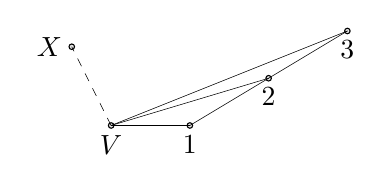
\begin{tikzpicture}
    \tkzDefPoint(0,0){v_1}
    \tkzDefPoint(1,0){v_2}
    \tkzDefPoint(2,0.6){v_3}
    \tkzDefPoint(3,1.2){v_4}
    \tkzDefPoint(-0.5,1){v_5}
    \tkzDrawPoints(v_1,v_2, v_3, v_4, v_5)
    \tkzDrawSegments(v_1,v_2 v_3,v_4  v_2,v_3 v_1,v_4 v_1,v_3)
    \tkzDrawSegments[dashed](v_1,v_5)
    \tkzLabelPoint[below](v_1){$V$}
    \tkzLabelPoint[below](v_2){1}
    \tkzLabelPoint[below](v_3){2}
    \tkzLabelPoint[below](v_4){3}
    \tkzLabelPoint[left](v_5){$X$}
    \end{tikzpicture}\\
    Wydłużamy ścieżkę $V$-1-2-3 o $X$.\\
\end{center}


\begin{problem}{2}
	W pewnym kraju jest $n \geqslant{3}$ miast, przy czym każde dwa są połączone drogą albo torami kolejowymi. Pewien turysta planuje wyruszyć z pewnego miasta, odwiedzić każde miasto dokładnie raz, a następnie powrócić do wyjściowego miasta. Wykazać, że może tak wybrać wyjściowe miasto i tak zaplanować swoją trasę, aby zmienić środek transportu co najwyżej raz.
\end{problem}

\noindent
Przekłóżmy zadanie na język teorii grafów. Miasta będa wierzchołkami, połączenie kolejowe niebieską krawędzią, a połączenie drogowe czerwoną.

\vspace{5px}

\noindent
Wykażemy tezę indukcyjnie. Zauważmy, że dla $n = 3$ jest ona trywialna. Gdy wszystkie krawędzie są tego samego koloru, to dowolne przejście spełnia warunki zadania. Gdy tak nie jest, to zaczynamy w wierzchołku, w którym schodzą się dwie krawędzie różnych kolorów i przechodzimy przez wszystkie krawędzie.

\vspace{5px}

\noindent
Wyróżnijmy pewien wierzchołek $v$. Wszystkie inne wierzchołki tworzą graf, który ma $n - 1$ wierzchołków, a więc możemy skorzystać z założenia indukcyjnego. Załóżmy, że krawędzie $d_1d_2$, $d_2d_3$, ..., $d_{k-1}d_1$ tworzą cykl spełniający warunki zadania. Gdy cykl ten jest jednokolorowy, to jeśli wstawimy $v$ między $d_1$ i $d_2$, to tak otrzymany cykl będzie spełniał założenia. 

\vspace{5px}

\noindent
Rozpatrzmy przypadek, w którym istnieje kolor $\mathcal{K}$, że tylko jedna krawędź jest koloru $x$. Załóżmy, bez straty ogólności, że $d_1d_2$ jest koloru $\mathcal{K}$, a inne krawędzie są innego koloru. Wtedy cykl $d_1v$, $vd_2$, $d_2d_3$, ..., $d_{k-1}d_1$ spełnia warunki zadania. 

\vspace{5px}

\begin{center}
    \begin{tikzpicture}
    \tkzDefPoint(0,0){v_1}
    \tkzDefPoint(2,0){v_2}
    \tkzDefPoint(2,1){v_4}
    \tkzDefPoint(3,0.5){v_3}
    \tkzDefPoint(0,1){v_5}
    \tkzDefPoint(-1,0.5){v_6}
    \tkzDefPoint(1,2){v}
    \tkzDrawPoints(v_1,v_2, v_3, v_4, v_5, v_6, v)
    \tkzDrawSegments(v_1,v_2 v_2,v_3 v_1,v_6 v_5,v_6 v,v_5)
    \tkzDrawSegments[dashed](v_4,v_5 v_3,v_4 v,v_4)
    \end{tikzpicture}
\end{center}


\noindent
Teraz przyjrzyjmy się przypadkowi, w którym każdy z kolorów wystepuje co najmniej dwukrotnie na rozpatrywanym cyklu.
Załóżmy więc bez straty ogólności, że $d_1d_2$ i $d_2d_3$ są czerwone, a $d_3d_4$ i $d_4d_5$ są niebieskie. Przyjmijmy, również bez straty ogólności, że $vd_3$ jest czerwona. Wtedy cykl $d_1d_2$, $d_2d_3$, $d_3v$, $vd_4$, $d_4d_5$, ..., $d_{k-2}d_{k-1}$, $d_{k-1}d_1$ spełnia warunki zadania.

\vspace{5px}

%Source: Tournament of the towns 1986
\begin{problem}{3}
	W pewnym turnieju bierze udział $40$ drużyn. Pierwszego dnia każda z drużyn rozegrała jeden mecz. Drugiego dnia również. Wykazać, że istnieje pewne $20$ drużyn, takich, że każde dwie spośród nich jeszcze nie grały ze sobą meczu.
\end{problem}

\noindent
Rozpatrzmy graf, w którym wierzchołkami będą drużyny. Krawedź będzie istnieć wtedy i tylko wtedy, gdy drużyny odpowiadające jej końcą rozegrały ze sobą mecz. Zauważmy, że warunek z zadania jest równoważny faktowi, że stopień każdego wierzchołka jest równy~2. 

Wybierzmy pewien wierzchołek i rozpocznijmy w nim spacer po grafie. Będziemy przechodzić do następnych wierzchołków krawędziami, którymi jeszcze nie szliśmy. Łatwo zauważyć, że musimy w ten sposób otrzymać cykl, w którym każdy wierzchołek odwiedzamy co najwyżej raz. Skoro stopień każdego z wierzchołków wynosi $2$, to żaden z wierzchołków tego cyklu nie ma krawędzi łączącej go z jakimkolwiek wierzchołkiem spoza tego cyklu. Wykonując analogiczne spacery startując z nieodwiedzonych jeszcze wierzchołków - o ile takowe istnieją - otrzymamy, że graf jest sumą rozłącznych cykli.

Pokolorujmy każdą z krawędzi na czerwono, jeśli mecz odbył się pierwszego dnia, lub na zielono, jeśli odbył się drugiego dnia. Zauważmy, że z każdego wierzchołka wychodzi jedna zielona i jedna czerwona krawędź. Stąd w każdym cyklu krawędzie na przemian: zielona, czerwona, zielona, czerwona, ... itd. Stąd każdy z cykli jest parzystej długości. 

\begin{center}
    \begin{tikzpicture}
    \tkzDefPoint(0,0){v_1}
    \tkzDefPoint(2,0){v_2}
    \tkzDefPoint(2,2){v_4}
    \tkzDefPoint(3,1){v_3}
    \tkzDefPoint(0,2){v_5}
    \tkzDefPoint(-1,1){v_6}
    \tkzDrawPoints(v_1,v_2, v_3, v_4, v_5, v_6)
    \tkzDrawSegments(v_1,v_2 v_3,v_4 v_5,v_6)
    \tkzDrawSegments[dashed](v_2,v_3 v_4,v_5 v_1,v_6)

    \tkzDefPoint(4,0){v_1}
    \tkzDefPoint(6,0){v_2}
    \tkzDefPoint(6,2){v_3}
    \tkzDefPoint(4,2){v_4}
    \tkzDrawPoints(v_1,v_2, v_3, v_4)
    \tkzDrawSegments(v_1,v_2 v_3,v_4)
    \tkzDrawSegments[dashed](v_2,v_3 v_4,v_1)
    \end{tikzpicture}
\end{center}

W każdym z cykli długości parzystej możemy wybrać połowę jego wierzchołków, aby żadne dwa z nich nie grały ze sobą meczu. Wybierając takie wierzchołki dla każdego z cykli otrzymamy połowę wierzchołków z całego grafu, które nie są połączone ze sobą. Odpowiadające im $20$ drużyn spełniają warunki zadania.

\vspace{5px}

\newpage

%Source: Tournament of the Towns Senior-O Spring 2011 P5
\begin{problem}{4}
	Dany jest graf spójny zawierający parzystą liczbę wierzchołków. Wykazać, że możemy pokolorować niektóre z jego krawędzi, aby z każdego wierzchołka wychodziła nieparzysta liczba pokolorowanych krawędzi.
\end{problem}

\noindent
Rozpatrzmy dwa wierzchołki $u$ i $v$. Skoro graf jest spójny, to istnieje różnowierzchołkowa ścieżka między tymi wierzchołkami. Zmieńmy stan -- z pokolorowanej na niepokolorowaną i na odwrót --  każdej z krawędzi na tej ścieżce. Zauważmy, że parzystość liczby kolorowych krawędzi wychodzących z każdego wierzchołka wewnątrz ścieżki nie ulegnie zmianie. Natomiast parzystość liczby kolorowych krawędzi wychodzących z $u$ i z $v$ się zmieni. Czyli jesteśmy w stanie zmienić parzystość liczby kolorowych krawędzi wychodzących z dowolnych dwóch wierzchołków. Skoro liczba wierzchołków w grafie jest liczbą parzystą, to możemy podzielić je w dowolny sposób na pary i zastosować wskazany wyżej algorytm dla każdej z nich. W ten sposób uzyskamy szukane kolorowanie.

\vspace{5px}

\begin{problem}{5}
	W pewnym grafie o $n$ wierzchołkach ich stopnie wynoszą odpowiednio $d_1$, $d_2$, ..., $d_n$. Udowodnić, że istnieje taki podzbiór co najmniej $\sum^{n}_{i = 1} \frac{1}{1 + d_i}$ jego wierzchołków, że żadne dwa z nich nie są połączone krawędzią.
\end{problem}

\noindent
Rozpatrzmy wierzchołek o największym stopniu. Wyróżnijmy go i usuńmy go wraz ze wszystkimi sąsiadującymi wierzchołkami. Bez straty ogólności $d_1 \geqslant d_2 \geqslant ... \geqslant d_{d_1 + 1}$ to będą stopnie usuniętych wierzchołków. Wówczas rozpatrywana suma ułamków zmniejszy się o sumę
\[
	\sum^{d_1 + 1}_{i = 0} \frac{1}{d_i + 1} \geqslant \sum^{d_1 + 1}_{i = 0} \frac{1}{d_1 + 1} = 1.
\]
Także po usunięciu tych wierzchołków inne stopnie mogą się zmniejszyć, ale to jeszcze bardziej zmniejszy naszą sumę.

Wykazaliśmy, że usuwając pewien wierzchołek i jego sąsiadów, zmiejszamy rozpatrywaną sumę o co najwyżej $1$. Powtarzając ten algorytm, wykonamy co najmniej $\sum^{n}_{i = 1} \frac{1}{1 + d_i}$ usunięć. Biorąc pod uwagę wyróżnione wierzchołki otrzymamy zbiór spełniający warunki zadania.

\vspace{5px}

%Source: https://artofproblemsolving.com/community/c6h455746p2560781
\begin{problem}{6}
	Hydra składa się z pewnej liczby głów, z której niektóre są połączone szyjami. Herkulers może odciąć wszystkie szyje wychodzące z pewnej głowy, jednak wówczas z tamtej głowy wyrastają szyję, którą łączą ją z głowami, z którymi nie była ona wcześnie połączona. Hydra jest pokonana, gdy rozpada się na dwie rozłączne części. Wyznaczyć najmniejsze $N$, że Herkules jest w stanie pokonać dowolną hydrę składającą się ze $100$ szyi.
\end{problem}

\noindent
Wykażemy, że $N = 10$. Oczywiście rozpatrzamy dany problem w języku teorii grafów. Rozpatrzmy dwa przypadki.

Jeśli istnieje wierzchołek o stopnie nie większym niż $10$, to Herkules może odciąć każdego z jego sąsiadów i wówczas ten wierzchołek nie będzie miał już żadnych sąsiadów. W ten sposób może osiągnąć swój cel.

Załóżmy teraz, że każdy wierzchołek ma stopień co najmniej $11$. Oznaczmy liczbę wierzchołków jako $K$. Wówczas liczba krawędzi wynosi co najmniej $\frac{11K}{2}$. Skoro jest ona równa $100$, to otrzymujemy $K \leqslant 18$. Zauważmy, że po wykonaniu odcięcia wierzchołka o stopniu co najmniej $11$, będzie on miał stopień co najwyżej $18 - 11 - 1 = 6$. Wówczas stosując procedurę analogiczną do poprzedniego prypadku otrzymamy $6 + 1 = 7$ łacznych cięć.


Pozostaje wskazać przykład grafu, którego nie da rozciąć się w mniej niż $10$ ruchach. Zauważmy, że graf $K_{a,b}$ może zostać przekształcony na jeden z grafów $K_{a - 1,b + 1}$ lub $K_{a + 1,b - 1}$. Rozpatrując graf $K_{10,10}$ otrzymujemy szukany przykład.

\newpage
\solutions{Indukcja matematyczna 2}

\begin{problem}{1}
	Udowodnić, że za pomocą monet trzyzłotowych i pięciozłotowych można zapłacić każdą kwotę większą niż $7$ złotych, bez konieczności wydawania reszty.
\end{problem}

\noindent
Najpierw zauważymy, że skoro zachodzą równości
\[
	8 = 5 + 3, \quad 9 = 3 + 3 + 3, \quad 10 = 5 + 5,
\]
skąd wynika, że kwoty 8, 9 i 10 złotych da się zapłacić bez wydawania reszty.

\vspace{5px}

\noindent
Załóżmy, że dla pewnej liczby całkowitej $k \geqslant 11$, da się we wspomniany sposób zapłacić wszystkie kwoty większe od $7$ złotych, ale nie większe niż $k$. Wówczas w szczególności da się zapłacić kwotę $(k + 1) - 3 \geqslant 8$ złotych. Dokładając jedną monetę trzyzłotową otrzymujemy szukane przestawienie kwoty $k + 1$ złotych. Z zasady indukcji matematycznej wynika teza.

\begin{problem}{2}
	Dana jest liczba naturalna $n$. Niech $\mathcal{S}$ będzie zbiorem wszystkich punktów postaci $(a, b)$, gdzie $a$ i $b$ są liczbami ze zbioru $\{0, 1, 2, ..., n\}$ oraz $a + b \leqslant n$. 

	\begin{center}
	\begin{tikzpicture}[scale = 0.5]
	    \tkzDefPoint(0,0){v_1}
	    \tkzDefPoint(1,0){v_2}
	    \tkzDefPoint(2,0){v_3}
	    \tkzDefPoint(3,0){v_4}
	    \tkzDefPoint(0,1){v_5}
	    \tkzDefPoint(1,1){v_6}
	    \tkzDefPoint(2,1){v_7}
	    \tkzDefPoint(0,2){v_8}
	    \tkzDefPoint(1,2){v_9}
	    \tkzDefPoint(0,3){v_{10}}
	    \tkzDrawPoints(v_1,v_2, v_3, v_4, v_5, v_6, v_7, v_8, v_9, v_{10})
	\end{tikzpicture}\\
	\vspace{5px}
	Przykład dla $n = 3$.
	\end{center}

	\noindent
	Wykazać, że jeśli pewien zbiór prostych zawiera każdy z tych punktów, to zawiera on co najmniej $n + 1$ prostych. 
\end{problem}

\noindent
Zauważmy, że dla $n = 0$ teza jest trywialna -- zbiór $\mathcal{S}$ zawiera jedynie punkt $(0, 0)$ i do jego pokrycia jest potrzebna jedna prosta. Rozumując indukcyjnie, załóżmy, że teza zachodzi dla pewnej liczby naturalnej $n$. Wykażmy, że jest prawdziwa również dla $n + 1$.

\vspace{5px}

\begin{center}
	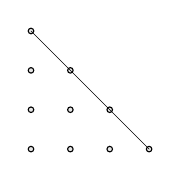
\begin{tikzpicture}[scale = 0.5]
	    \tkzDefPoint(0,0){v_1}
	    \tkzDefPoint(1,0){v_2}
	    \tkzDefPoint(2,0){v_3}
	    \tkzDefPoint(3,0){v_4}
	    \tkzDefPoint(0,1){v_5}
	    \tkzDefPoint(1,1){v_6}
	    \tkzDefPoint(2,1){v_7}
	    \tkzDefPoint(0,2){v_8}
	    \tkzDefPoint(1,2){v_9}
	    \tkzDefPoint(0,3){v_{10}}
	    \tkzDrawPoints(v_1,v_2, v_3, v_4, v_5, v_6, v_7, v_8, v_9, v_{10})
	    \tkzDrawSegment(v_4,v_{10})
	\end{tikzpicture}
	\hspace{40px}
	\begin{tikzpicture}[scale = 0.5]
	    \tkzDefPoint(0,0){v_1}
	    \tkzDefPoint(1,0){v_2}
	    \tkzDefPoint(2,0){v_3}
	    \tkzDefPoint(3,0){v_4}
	    \tkzDefPoint(0,1){v_5}
	    \tkzDefPoint(1,1){v_6}
	    \tkzDefPoint(2,1){v_7}
	    \tkzDefPoint(0,2){v_8}
	    \tkzDefPoint(1,2){v_9}
	    \tkzDefPoint(0,3){v_{10}}
	    \tkzDefPoint(3,-0.5){a}
	    \tkzDefPoint(3,0.5){b}
	    \tkzDrawPoints(v_1,v_2, v_3, v_4, v_5, v_6, v_7, v_8, v_9, v_{10})
	    \tkzDrawSegments(v_1,v_{10} v_2,v_9 v_3,v_7 a,b)
	\end{tikzpicture}
\end{center}

\noindent
Weźmy dowolny zbiór prostych, które przykrywają każdy z punktów zbioru $\mathcal{S}$ dla $n + 1$. Wyróżnijmy punkty $(a, b)$, dla których zachodzi równość $a + b = n + 1$. Zauważmy, że wszystkie te punkty leżą na jednej prostej. Rozpatrzmy dwa przypadki
\begin{enumerate}
	\item Istnieje prosta $l$, która przykrywa pewne dwa wyróżnione punkty. Wówczas przykrywa ona wszystkie wyróżnione punkty i żadnego innego punktu ze zbioru $\mathcal{S}$. Zauważmy, że dla zbioru $\mathcal{S}$ z usuniętymi wyróżnionymi punktami, możemy zaaplikować założenie indukcyjne. Wynika z niego, że do pokrycia rozpatrywanych punktów potrzeba co najmniej $n$ prostych. Dokładając prostą $l$ otrzymujemy, że łącznie prostych jest co najmniej $n + 1$.
	\item Żadne dwa wyróżnione punkty nie są przykryte przez jedną prostą. Skoro jest $n + 1$ punktów, to do ich przykrycia będzie potrzebnych $n + 1$ prostych. W szczególności do pokrycia zbioru $\mathcal{S}$ potrzeba $n + 1$ prostych.
\end{enumerate}


\begin{problem}{3}
	Wykazać, że istnieje taka dodatnia liczba całkowita, że jest ona podzielna przez $2^{1000}$, oraz ma w zapisie dziesiętnym jedynie cyfry $1$ i $2$.
\end{problem}

\noindent
Powiemy, że liczba naturalna $x$ jest \textit{dobra}, jeśli ma dokładnie $n$ cyfr, z których każda jest jedynką lub dwójką, oraz $x$ jest podzielna przez liczbę $2^n$. 

\vspace{5px}
\noindent
Wykażemy indukcyjnie, że dla dowolnej dodatniej liczby całkowitej $n$, istnieje $n$ cyfrowa liczba dobra. Zauważmy, że liczba $2$ jest liczbą dobrą. Załóżmy, że dla pewnego $n$ istnieje $n$-cyfrowa liczba dobra -- nazwijmy ją $2^n \cdot a_n$. Wykażemy wówczas, że istnieje $n + 1$-cyfrowa liczba dobra.

\vspace{5px}
\noindent
Rozpatrzmy dwa przypadki
\begin{enumerate}
	\item Jeśli liczba $a_n$ jest nieparzysta, to weźmy liczbę 
	\[
		10^{n} + 2^n \cdot a_n = 2^n\left(5^n + a_n\right).
	\]
	Powstaje ona przez doklejenie do $2^n \cdot a_n$ cyfry $1$ z lewej strony.
	W nawiasie jest suma dwóch liczb nieparzystych, a więc jest ona parzysta. Stąd $10^{n} + 2^n \cdot a_n $ jest podzielna przez $2^{n + 1}$.
	\item Gdy liczba $a_n$ jest parzysta, to rozpatrzmy liczbę 
	\[
		2 \cdot 10^{n} + 2^n \cdot a_n = 2^n\left(2 \cdot 5^n + a_n\right).
	\]
	Powstaje ona przez doklejenie do $2^n \cdot a_n$ cyfry $2$ z lewej strony.
	W nawiasie jest suma dwóch liczb parzystych, a więc jest ona parzysta. Więc $2 \cdot 10^{n} + 2^n \cdot a_n $ jest podzielna przez $2^{n + 1}$.
\end{enumerate}
W każdym z przypadków rozpatrywana liczba jest $n + 1$-cyfrową liczbą dobrą. Kończy to dowód indukcyjny. Biorąc liczbę dobrą, która ma $1000$ cyfr. Jest ona podzielna przez $2^{1000}$ oraz składa się wyłącznie z cyfr $1$ i $2$.

\begin{remark}
	Liczby dobre wygenerowane za pomocą powyższego rozumowania to
	\[
		2, \; 12, \; 112, \; 2112, \; 22112, \; ...
	\]
\end{remark}

\begin{problem}{4}
	Niech $k$ będzie dodatnią liczbą całkowitą. Na przyjęciu spotkało sie $n \geqslant 2$ gości, spośród których niektórzy znają się. Okazało się, że dla każdego niepustego podzbioru gości $A$ istnieje osoba, która zna co najwyżej $k$ osób z $A$. Podzbiór gości, spośród których każde dwie się znają, nazywamy \textit{kilką}. Wykazać, że istnieje co najwyżej $2^k \cdot n$ klik.
\end{problem}

\noindent
Zadanie rozwiążemy indukując się po $n$. Jeśli $n = 2$, to teza jest trywialna -- trzeba wykazać, że istnieją co najwyżej 4 kliki, a są 4 możliwe podzbiory zbiorów gości. W dalszej części rozwiązania zakładamy, że $n \geqslant 3$.

\vspace{10px}

\noindent
Na mocy założenia zadania zastosowanego dla zbioru wszystkich $n$ osób, istnieje pewna osoba $X$, która ma co najwyżej $k$ zajomych. Usuwając osobę $X$, założenie z zadania nadal będzie zachodzić dla pozostałych osób. Na mocy założenia indukcyjnego liczba klik, które nie zawierają $X$ wynosi $2^k \cdot (n - 1)$. 

Klika, która zawiera $X$, nie może zawierać osoby, której $X$ nie zna. Musi więc składać się z $X$ oraz pewnego podzbioru znajomych $X$. Skoro $X$ ma co najwyżej $k$ znajomych, to tych podzbiorów jest co najwyżej $2^k$.

\begin{center}
	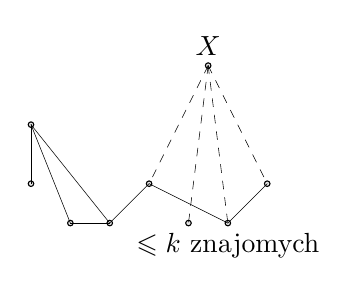
\begin{tikzpicture}[scale = 0.5]
	    \tkzDefPoint(2.5,4){v}
	    \tkzDefPoint(-2,1){x_0}
	    \tkzDefPoint(-1,0){x_1}
	    \tkzDefPoint(0,0){x_2}
	    \tkzDefPoint(-2,2.5){x_3}
	    \tkzDefPoint(1,1){v_2}
	    \tkzDefPoint(2,0){v_3}
	    \tkzDefPoint(3,0){v_4}
	    \tkzDefPoint(4,1){v_5}
	    \tkzDefPoint(2,0){a}
	    \tkzDefPoint(4,0){b}
	    \tkzDrawPoints(v, x_0, x_1, x_2, x_3, v_2, v_3, v_4, v_5)
	    \tkzDrawSegments(v_2,v_4 v_4,v_5 x_1,x_2 x_2,x_3 x_3,x_0 x_1,x_3 x_2,v_2)
	    \tkzDrawSegments[dashed](v,v_2 v,v_3 v,v_4 v,v_5)
	    \tkzLabelSegment[below](a,b){$\leqslant k$ znajomych}
	    \tkzLabelPoint[above](v){$X$}
	\end{tikzpicture}
\end{center}

\vspace{5px}

\noindent
Łącząc powyższe wnioski otrzymujemy, że klik jest co najmniej $2^k \cdot (n - 1) + 2^k = 2^k \cdot n$. Z zasady indukcji matematycznej wynika teza.

\begin{problem}{5}
	Znajdź wszystkie funkcje $f$ z dodatnich liczb całkowitych w dodatnie liczby całkowite, które dla każdej liczby dodatniej całkowitej $n$ spełniają nierówności
	\[
		(n - 1)^2 < f(n)f(f(n)) < n^2 + n.
	\]
\end{problem}

\noindent
Podstawiając do wyjściowego równania $n = 1$ otrzymamy
\[
	0 < f(1)f(f(1)) < 2,
\]
skąd $f(1) = f(f(1)) = 1$.
Wykażemy indukcyjnie, że $f(n) = n$. Załóżmy, że równość $f(k) = k$ zachodzi dla wszystkich dodatnich liczb całkowitych $k$ mniejszych od $n$. 

\begin{enumerate}
	\item Jeśli $f(n) \leqslant n - 1$, to z założenia indukcyjnego $f(f(n)) = f(n)$. Wówczas
	\[
		f(n)f(f(n)) = f(n)^2 \leqslant (n - 1)^2,
	\]
	co daje sprzeczność.
	\item Gdy $f(n) \geqslant n + 1$, to skoro
	\[
		f(n)f(f(n)) < n^2 + n,
	\]
	to $f(f(n)) < n$, czyli $f(f(n)) \leqslant n - 1$. Stąd na mocy założenia indukcyjnego $f(f(f(n))) = f(f(n))$. Wstawiając $f(n)$ zamiast $n$ do danej nierówności otrzymamy
	\[
		(f(n) - 1)^2 < f(f(f(n)))f(f(n)) = f(f(n))^2 \leqslant (n - 1)^2,
	\]
	co przeczy temu, że $f(n) \geqslant n + 1$.
\end{enumerate}

\noindent
Stąd musi zajść $f(n) = n$, co kończy rozumowanie indukcyjne.

\begin{problem}{6}
	Niech $\mathcal{R}$ będzie rodziną zbiorów $1000$-elementowych. Moc $\mathcal{R}$ jest większa niż $1000 \cdot 999^{1000}$ Wykazać, że istnieje $1000$-elementowa rodzina $\mathcal{G}$, będąca podrodziną $\mathcal{R}$, oraz taki zbiór $X$, że dla dowolnych zbiorów $A, B \in \mathcal{R}$ zachodzi $A \cap B = X$.
\end{problem}

\noindent
Wykażemy nieco ogólniejszą i mocniejszą wersję tezy.

\vspace{10px}

\noindent
Niech $\mathcal{R}$ będzie rodziną zbiorów $n$-elementowych. Moc $\mathcal{R}$ jest większa niż $n! \cdot k^{n}$ Wówczas istnieje $k+1$-elementowa rodzina $\mathcal{G}$, będąca podrodziną $\mathcal{R}$, oraz taki zbiór $X$, że dla dowolnych zbiorów $A, B \in \mathcal{R}$ zachodzi $A \cap B = X$.

\vspace{10px}

\noindent
Będziemy przeprowadzać indukcję po liczbie $n$. Dla $n = 1$ moc $\mathcal{R}$ to co najmniej $k + 1$. Każdy ze zbiorów zawiera jeden element, więc każde dwa mają puste przecięcie. Stąd biorąc całą rodzinę $\mathcal{R}$ oraz $X = \emptyset$ otrzymujemy tezę.

\vspace{10px}

\noindent
Rozpatrzmy największą podrodzinę $\mathcal{H}$ rodziny $R$, że dowolne dwa jej podzbiory mają puste przecięcie. Moc $\mathcal{H}$ jest nie większa niż $k$, gdyż w przeciwnym przypadku biorąc rodzinę $\mathcal{H}$ i $X = \emptyset$ otrzymamy tezę. Stąd każdy zbiór $A \in \mathcal{R}$ ma niepuste przecięcie z pewnym ze zbiorów z rodziny $\mathcal{H}$.

\vspace{10px}

\noindent
Łącznie zbiory należące do rodziny $\mathcal{H}$ zawierają co najwyżej $k \cdot n$ elementów -- jest co najwyżej $k$ zbiorów $n$-elementowych. Skoro wszystkich zbiorów należących do $\mathcal{R}$ jest więcej niż $n! \cdot k^{n}$, to istnieje element $a$, który należy do
\[
	\frac{n! \cdot k^{n}}{n \cdot k} = (n - 1)! \cdot k^{n - 1}
\]
zbiorów.

\vspace{10px}

\noindent
Rozpatrując zbiory zawierające element $a$, następnie usuwając go z każdego z nich, otrzymamy więcej niż $(n - 1)! \cdot k^{n - 1}$ zbiorów, które zawierają po $n - 1$ elementów. Można więc skorzystać z założenia indukcyjnego. Istnieje więc pewien zbiór $X$ oraz pewna podrodzina rozpatrywanej rodziny zbiorów, że $X$ jest przecięciem dowolnych zbiorów należących do danej podrodziny. Dokładając ponownie do każdego z tych zbiorów element $a$ otrzymujemy tezę.





\newpage
\solutions{Podzielności}

\begin{problem}{1}
	Wyznaczy wszystkie dodatnie liczby całkowite $n$, które są podzielne przez liczbę~$\left\lfloor \sqrt{n} \right\rfloor$.
\end{problem}

\answer{Jedynymi liczbami spełniającymi warunki zadania są liczby postaci $k^2$, $k^2 + k$ oraz $k^2 + 2k$ dla pewnej liczby całkowitej $k$.}

\noindent
Rozpatrzmy taką dodatnią liczbę całkowitą $k$, że
\[
	(k + 1)^2 > n \geqslant k^2.
\]
Innymi słowy $k$ jest największą liczbą całkowitą, taką, że $k^2$ jest nie większe niż $n$. Wówczas
\[
	k + 1 > \sqrt{n} \geqslant k,
\]
czyli $\left\lfloor \sqrt{n} \right\rfloor = k$. Jedynymi liczbami w przedziale $[k^2, (k + 1)^2)$, które są podzielne przez $k$ są $k^2$, $k^2 + k$ i $k^2 + 2k$.


\begin{problem}{2}
	Dane są dodatnie liczby całkowite $a$, $b$, $c$, że liczba $a^b$ dzieli $b^c$ oraz $a^c$ dzieli $c^b$. Wykazać, że $a^2$ dzieli $bc$.
\end{problem}

\noindent
Niech $p$ będzie dowolną liczbą pierwszą.
Z danych podzielności wynika, że
\[
	v_p(b^c) \geqslant v_p(a^b) \quad \text{oraz} \quad v_p(c^b) \geqslant v_p(a^c),
\]
czyli równoważnie
\[
	cv_p(b) \geqslant bv_p(a) \quad \text{oraz} \quad bv_p(c) \geqslant cv_p(a),
\]
Mamy więc
\[
	v_p(bc) = v_p(b) + v_p(c) = \frac{b}{c}v_p(a) +  \frac{c}{b}v_p(a) \geqslant 2\sqrt{\frac{b}{c} \cdot \frac{c}{b} \cdot v_p(a)^2} = 2v_p(a),
\]
z czego wynika teza.


\begin{problem}{3}
	Niech $1 = d_0 < d_1 < d_2 < ... < d_k = 4n$ będą kolejnymi dzielnikami liczby $4n$. Wykazać, że istnieje taka liczba $i$, dla której zachodzi równość $d_{i + 1} - d_i = 2$.
\end{problem}

\noindent
Załóżmy, że teza nie zachodzi -- wtedy musi zachodzić następujący fakt:
\begin{center} 
	Jeśli $d$ oraz $d + 2$ są dzielnikami liczby $4n$, to liczba $d + 1$ również. (*)
\end{center}
Wykażemy, że istnieje nieskończenie wiele takich liczb naturalnych $k$, że $2k$, $2k + 1$ oraz $2k + 2$ są dzielnikami liczby $n$. Na początku zauważmy, że $2$ i $4$ są dzielnikami $4n$. Z (*) liczba $3$ również nim będzie. 

\vspace{10px}

\noindent
Załóżmy więc, że dla pewnej liczby naturalnej $k$ liczby $2k$, $2k + 1$ oraz $2k + 2$ są dzielnikami liczby $4n$. Wówczas jedna z liczb $2k$, $2k + 2$ nie jest podzielna przez $4$. Bez straty ogólności przyjmijmy, że jest to $2k$. Skoro $2k$ nie dzieli się przez $4$ i jest dzielnikiem liczby $4n$, to liczba $4k$ również będzie dzielnikiem liczby $4n$. 

Analogicznie postępując z liczbą $2n + 1$, która jest nieparzysta, otrzymamy, że również liczba $4k + 2$ jest dzielnikiem liczby $4n$. Z (*) mamy, że $4k + 1$ musi być dzielnikiem $4n$. Otrzymaliśmy większą trójkę $(4k, 4k + 1, 4k + 2)$ kolejnych dzielników liczby $4n$.

\vspace{10px}

\noindent
Możemy w ten sposób uzyskać dowolnie duże trójki kolejnych dzielników $4n$, co jest oczywistą sprzecznością, gdyż dzielniki te są nie większe niż $4n$.

\vspace{10px}

\begin{problem}{4}
	Znajdź wszystkie pary $(a, b)$ liczb całkowitych dodatnich, większych od 1, dla których obie liczby
	\[
		\frac{a^3b - 1}{a + 1} \quad \text{oraz} \quad \frac{b^3a + 1}{b - 1}
	\]
	są całkowite
\end{problem}

\answer{
	Szukanymi parami liczb są $a = 2$ i $b = 2$, $a = 1$ i $b = 3$, oraz $a = 3$ i $b = 3$.
}

\noindent
Zauważmy, że 
\[
	\frac{a^3b - 1}{a + 1} = a^2b - \frac{a^2b + 1}{a + 1} = a^2b - ab + \frac{ab - 1}{a + 1} = a^2b - ab + b - \frac{b + 1}{a + 1}.
\]
Wynika stąd, że liczba $b + 1$ jest podzielna przez liczbę $a + 1$. Mamy również
\[
	\frac{b^3a + 1}{b - 1} = b^2a + \frac{b^2a + 1}{b - 1} = b^2a + ab + \frac{ab + 1}{b - 1} = b^2a - ab + a + \frac{a + 1}{b - 1},
\]
czyli $a + 1$ jest podzielna przez liczbę $b - 1$. 

\vspace{10px}

\noindent
Liczba $a + 1$ jest dzielnikiem liczby $b + 1$ oraz wielokrotnością liczby $b - 1$. Stąd liczba $b + 1$ jest podzielna przez liczbę $b - 1$. Zauważmy, że jeśli $b \geqslant 4$, to
\[
	b + 1 > b - 1 > \frac{b + 1}{2},
\]
co przeczy wspomnianej podzielności.
Więc $b = 2$ lub $b = 3$. Jeśli $b = 2$, to $a + 1$ jest dzielnikiem $3$. Skoro jest większe od 1, to musi być równe 3, skąd $a = 2$. Dla $b = 3$ mamy, że $a + 1$ musi być dzielnikiem $4$ i musi być podzielne przez $2$. Stąd $a = 1$ lub $a = 3$. 

\begin{problem}{5}
	Dane są parami różne dodatnie liczby całkowite $a$, $b$, $c$ oraz nieparzysta liczba pierwsza $p$, że liczby
	\[
		ab + 1, \; bc + 1, \; ca + 1
	\] 
	są podzielne przez $p$. Wykazać, że
	\[
		\frac{a + b + c}{3} \geqslant p + 2.
	\]
\end{problem}

\noindent
Zauważmy, że skoro $p \mid ab + 1$ oraz $p \mid bc + 1$, to
\[
	p \mid (ab + 1) - (bc + 1) = b(a - c).
\]
Skoro $p$ jest liczbą pierwszą, to dzieli ona $b$ lub dzieli ona $a - c$. Gdyby dzieliła liczbę $b$, to wówczas nie mogła by dzielić liczby $bc + 1 \equiv 1 \pmod{p}$. Stąd $p \mid a - c$, czyli 
\[
	a \equiv c \pmod{p}.
\] 
Rozumując analogicznie dla podzielności $p \mid bc + 1$ i $p \mid ca + 1$, otrzymamy $a \equiv b \pmod{p}$. Stąd
\[
	a \equiv b \equiv c \pmod{p}.
\]
Pozostaje zauważyć, że $a \not\equiv 1 \pmod{p}$, bo w przeciwnym wypadku 
\[
	ab + 1 \equiv a^2 + 1 \equiv 2 \pmod{p}.
\]
Przyjmijmy, że $2 \leqslant a < b < c$. Skoro dają one tę samą resztę z dzielenia przez $p$, to różnią się o wielokrotność liczby $p$, czyli co najmniej o $p$. Stąd
\[
	b \geqslant a + p \quad \text{oraz} \quad c \geqslant b + p \geqslant a + 2p,
\]
czyli
\[
	\frac{a + b + c}{3} \geqslant \frac{a + a + p + a + 2p}{3} = p + a \geqslant p + 2.
\]

\begin{problem}{6}
	Niech $a$ i $k$ będą pewnymi dodatnimi liczbami całkowitymi o tej własności, że dla dowolnej dodatniej liczby całkowitej $n$ istnieje liczba całkowita $b$, że
	\[
		n \mid a - b^k.
	\]
	Wykazać, że $a = c^k$ dla pewnej liczby całkowitej $c$.
\end{problem}

\noindent
\textit{Sposób 1}

\vspace{10px}

\noindent
Rozpatrzmy dowolną liczbę pierwszą $p$. Wykażemy, że $k \mid v_p(a)$, z czego wyniknie teza. Załóżmy nie wprost, że $v_p(a) = x \cdot k + r$, gdzie $x$ i $0 < r < k$ są dodatnimi liczbami całkowitymi. Weźmy $n = p^{xk + k}$. Wówczas istnieje takie $b$, że
\[
	p^{xk + k} \mid a - b^k.
\]
Zauważmy, że skoro $v_p(b^k)$ jest podzielne przez $k$, to może być albo nie mniejsze niż $xk + k$, albo nie większe niż $xk$. W obu przypadkach liczby $b^k$ i $a$ mają różne $v_p$, przy czym mniejsze z nich jest ściśle mniejsze niż $xk + k$. Na mocy Lematu 4 otrzymujemy 
\[
	v_p(a - b^k) = min(v_p(a), v_p(b^k)) < xk + k.
\]
Jest to sprzeczność z wyżej opisaną podzielnością.

\vspace{10px}

\noindent
\textit{Sposób 2}

\vspace{10px}

\noindent
Weźmy $n = a^2$. Wówczas na mocy założenia istnieją takie liczby całkowite $b$ oraz $d$, że
\[
	a - b^k = da^2,
\]
\[
	a(ad + 1) = b^k.
\]
Skoro $\mathrm{NWD}(a, ad + 1) = 1$, a iloczyn tych liczb jest $k$-tą potęgą liczby całkowitej, to każda z tych liczb jest $k$-tą potęgą liczby całkowitej.

\vspace{10px}


\newpage
\solutions{Gry}

%Source: https://om.mimuw.edu.pl/static/app_main/problems/om67_1.pdf Poland 2016 P1
\begin{problem}{1}
	Na tablicy napisano liczbę całkowitą dodatnią. W każdym ruchu zmazujemy napisaną liczbę $n$ na tablicy i piszemy nową liczbę. Jeśli $n$ była parzysta to piszemy na tablicy liczbę $\frac{1}{2}n$. Jeśli zaś liczba $n$ była nieparzysta, to zapisujemy jedną z liczb $3n - 1$ lub $3n + 1$. Czy -- niezależnie od tego, jaką liczbę zapisano na początku -- możemy, po skończenie wielu krokach, uzyskać na tablicy jedynkę?
\end{problem}

\answer{Jest to możliwe.}

\noindent
Wykażemy, że jeśli na tablicy znajduje się liczba $n \geqslant 2$, to zawsze jesteśmy w stanie sprawić, aby pojawiła się na tablicy dodatnia liczba całkowitej mniejsza od $n$. Rozpatrzmy dwa przypadki
\begin{itemize}
	\item Jeśli $n$ jest liczbą parzystą, to wystarczy zapisać liczbę $\frac{1}{2}n < n$.
	\item Gdy $n$ jest nieparzysta, to obie z liczb $3n + 1$ i $3n - 1$ są parzyste. Skoro różnią się o 2, to jedna z nich będzie liczbą podzielną przez $4$. Zapisujemy ją na tablicy, a następnie w dwóch kolejnych ruchach zapisujemy liczbę dwa razy mniejszą. Otrzymana liczba wyniesie co najwyżej
	\[
		\frac{3n + 1}{4} < \frac{4n}{4} = n.
	\]
\end{itemize}
Jako, że nie można ciągle zapisywać liczby mniejszej, gdyż zapisać można tylko liczby dodatnie całkowite, toteż kiedyś musimy zapisać liczbę $1$.

%Source: Lithuania 2010
% http://refkol.ro/matek/mathbooks/Grupe%20de%20performanta/Chapter5%20Games%20Aug%202014.pdf EX 9
\begin{problem}{2}
	W lewym dolnym rogu planszy $m \times n$ stoi pionek. W każdym ruchu może zostać on przesunięty o dowolną liczbę pól w górę lub o dowolną liczbę pól w prawo. Wygrywa gracz, który postawi figurę w prawym górnym rogu. Rozstrzygnąć dla jakich wartości $(m, n)$ pierwszy gracz ma strategię wygrywającą.
\end{problem}

\answer{Pierwszy gracz ma strategię wygrywającą wtedy i tylko wtedy, gdy $m \neq n$.}

\noindent
Analiza przykładowej planszy $7 \times 5$ została zobrazowana na poniższej tabelce. Litera $P$ oznacza, że jeśli pionek znajduje się na danym polu, to jest to stan przegrywający. Analogicznie $W$ oznacza stan wygrywający. Pole w prawym górnym rogu jest oczywiście stanem przegrywającym, gdyż jeśli przed ruchem tam znajduje się pionek, to gracz, którego jest kolej przegrał. Rozumując analogicznie jak w Przykładzie 2 otrzymamy poniższą tabelkę.
\begin{center}
\begin{tabular}{ |c|c|c|c|c|c|c|} 
 \hline
 W & W & W & W & W & W & P \\ 
 \hline
 W & W & W & W & W & P & W \\ 
 \hline
 W & W & W & W & P & W & W \\ 
 \hline
 W & W & W & P & W & W & W \\ 
 \hline
 W & W & P & W & W & W & W \\ 
 \hline
\end{tabular}
\end{center}

\noindent
Przejdźmy do rozwiązania zadania. Przyjmijmy, że pole w prawym górnym rogu ma współrzędne $(1, 1)$. Wówczas twierdzimy, że pole postaci $(a, b)$ jest przegrywające wtedy i tylko wtedy, gdy $a = b$. Wykażemy to indukcyjnie. Pole $(1, 1)$ jest przegrywające z definicji gry. Będziemy indukować się po sumie współrzędnych.

\vspace{10px}
\noindent
Jeśli gracz znajduje się na polu $(a, b)$, przy czym $a \neq b$, to może on przesunąć pionek na pole $(min(a, b), min(a, b))$, które jest stanem przegrywającym na mocy założenia indukcyjnego. Jeśli zaś gracz stoi na polu $(a, a)$, to jakiekolwiek pole, na które zostanie przesunięty pionek, nie będzie miało równych współrzędnych. Będzie więc stanem wygrywającym. Skoro więc każdy ruch doprowadza do stanu wygrywającego, to stan $(a, a)$ jest przegrywający.

\vspace{10px}
\noindent
Pozostaje tylko zauważyć, że dla $m \neq n$ wyjściowy stan jest wygrywający, a dla $m = n$ jest przegrywający. Toteż pierwszy gracz ma strategię wygrywającą jedynie dla $m \neq n$.

%Source: St. Petersburg 2001
% http://refkol.ro/matek/mathbooks/Grupe%20de%20performanta/Chapter5%20Games%20Aug%202014.pdf EX 10
\begin{problem}{3}
	Na tablicy zapisano liczbę $10000000$. W każdym ruchu, o ile przed nim była zapisana liczba $n$, gracz zastępuje ją liczbą $n - 1$ lub $\left\lfloor\frac{n + 1}{2}\right\rfloor$. Gracz, który zapisze liczbę $1$ wygrywa. Który z graczy – pierwszy czy drugi – ma strategię wygrywającą?
\end{problem}

\noindent
Wykażemy, że liczby parzyste są stanami wygrywającymi. Zauważmy, że liczba $2$ jest stanem wygrywającym, bo można ją zastąpić liczbą $2 - 1 = 1$. Załóżmy, że wszystkie liczby parzyste mniejsze niż $2a$ są stanami wygrywającymi.

\vspace{10px}
\noindent
Wykażemy, że liczba $2a + 2$ zapisana na tablicy również jest stanem wygrywającym. Rozpatrzmy dwa przypadki
\begin{itemize}
	\item Jeśli liczba $a + 1$ jest przegrywająca, to gracz wykonujący ruch może zastąpić liczbę $2a + 2$ przez liczbę $\left\lfloor\frac{2a + 3}{2}\right\rfloor = a + 1$ i w ten sposób umieścić przeciwnika w stanie przegrywającym.
	\item Załóżmy teraz, że liczba $a + 1$ jest wygrywająca. Wówczas gracz zastępuje liczbę $2a + 2$ liczbą $2a + 1$. Drugi gracz może zapisać albo liczbę $2a$ albo liczbę $a + 1$. Pierwsza z nich jest wygrywająca na mocy założenia indukcyjnego, a druga na mocy założenia z rozpatrywanego przypadku. W obu przypadkach gracz wykonujący ruch przy liczbie $2a + 2$ znów znajdzie się w stanie wygrywającym.
\end{itemize}

\vspace{10px}
\noindent
Wykazaliśmy, że liczby parzyste odpowiadają stanowi wygrywającemu, toteż skoro liczba $10000000$ jest parzysta, to pierwszy gracz ma strategię wygrywającą.

\begin{remark}
	Zauważmy, że nie wykazaliśmy nic o stanach, gdy na tablicy jest liczba nieparzysta. Nie było to jednak konieczne do rozwiązania powyższego zadania.
\end{remark}

\newpage

%Source: http://www.deltami.edu.pl/temat/matematyka/gry_zagadki_paradoksy/2017/12/31/Gry/ P4
\begin{problem}{4}
	Dwaj gracze na przemian stawiają kółko i krzyżyk w polach nieskończonej planszy. Gracz wygrywa, gdy istnieje kwadrat $2\times2$ ułożony z jego symboli. Wykazać, że drugi gracz może grać tak, aby pierwszy gracz nie był w stanie wygrać.
\end{problem}

\noindent
Podzielmy planszę na prostokąty $1 \times 2$ ułożone jak na rysunku -- boki wszystkich prostokątów o długości dwa są do siebie równoległe, ale żadne dwa z nich, które sąsiadują dłuższym bokiem, nie mają wspólnego wierzchołka.

\begin{center}
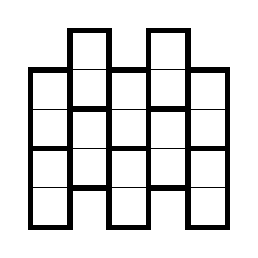
\begin{tikzpicture}[scale=0.5]

	\draw[line width=0.7mm] (0,0) -- (1,0) -- (1,2) -- (0,2) -- cycle;
	\draw (0,1) -- (1,1);
	\draw[line width=0.7mm] (0,2) -- (1,2) -- (1,4) -- (0,4) -- cycle;
	\draw (0,3) -- (1,3);

	\draw[line width=0.7mm] (1,3) -- (2,3) -- (2,5) -- (1,5) -- cycle;
	\draw (1,2) -- (2,2);
	\draw[line width=0.7mm] (1,1) -- (2,1) -- (2,3) -- (1,3) -- cycle;
	\draw (1,4) -- (2,4);

	\draw[line width=0.7mm] (2,0) -- (3,0) -- (3,2) -- (2,2) -- cycle;
	\draw (2,1) -- (3,1);
	\draw[line width=0.7mm] (2,2) -- (3,2) -- (3,4) -- (2,4) -- cycle;
	\draw (2,3) -- (3,3);

	\draw[line width=0.7mm] (3,3) -- (4,3) -- (4,5) -- (3,5) -- cycle;
	\draw (3,2) -- (4,2);
	\draw[line width=0.7mm] (3,1) -- (4,1) -- (4,3) -- (3,3) -- cycle;
	\draw (3,4) -- (4,4);

	\draw[line width=0.7mm] (4,0) -- (5,0) -- (5,2) -- (4,2) -- cycle;
	\draw (4,1) -- (5,1);
	\draw[line width=0.7mm] (4,2) -- (5,2) -- (5,4) -- (4,4) -- cycle;
	\draw (4,3) -- (5,3);
\end{tikzpicture}
\end{center}
Strategia drugiego gracza będzie następująca. Jeśli pierwszy gracz postawi swój symbol w jednym polu prostokąta, drugi gracz stawia swój symbol w drugim polu tego prostokąta. Kwadrat $2 \times 2$ zawiera pewien rozpatrywany prostokąt w całości. Jednak sytuacja, w której jeden prostokąt zawiera dwa jednakowe symbole się nie zdarzy. Stąd rozpatrywana strategia spełnia warunki zadania.


%Source: Russia 2021 10.5
% https://artofproblemsolving.com/community/c6h2534986p21567788
\begin{problem}{5}
	Nauczyciel wraz z 30 uczniami gra w grę na nieskończonej kartce w kratkę. Zaczyna on, po czym ruch wykonuje każdy z 30 uczniów, po czym znów nauczyciel, po czym uczniowie i tak dalej. W każdym ruchu należy pokolorować jeden z boków kratki, który nie został wcześniej pokolorowany. Nauczyciel wygrywa, gdy na planszy znajduje się prostokąt $2 \times 1$ lub $1 \times 2$, że wszystkie jego boki są pokolorowane, ale odcinek wewnątrz niego nie jest.
\end{problem}

\noindent
Strategia nauczyciela jest następująca. Rysuje on obwód kwadratu $n \times n$ w pierwszych $4n$ ruchach, w międzyczasie uczniowie zamalują $4n \cdot 30$ odcinków. Wówczas wewnątrz kwadratu znajduje się $2n(n - 1)$ odcinków. Jeśli $2n(n - 1) > 4n \cdot 30$, do czego wystarczy wziąć odpowiednio duże $n$, to liczba odcinków wewnątrz kwadratu będzie większa niż liczba odcinków pomalowana przez uczniów. Toteż będzie co najmniej jeden odcinek wewnątrz tego kwadratu, który nie jest pomalowany.

\begin{center}
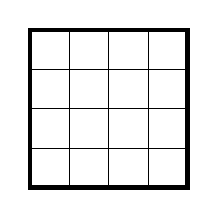
\begin{tikzpicture}[scale=0.5]
	\draw[line width = 0.6mm] (0,0)--(4,0)--(4,4)--(0,4)--cycle;
	\draw (0,1)--(4,1);
	\draw (0,2)--(4,2);
	\draw (0,3)--(4,3);
	\draw (1,0)--(1,4);
	\draw (2,0)--(2,4);
	\draw (3,0)--(3,4);
\end{tikzpicture}
\hspace{40px}
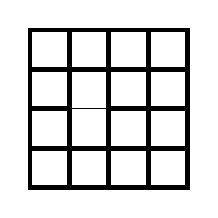
\begin{tikzpicture}[scale=0.5]
	\draw[line width = 0.6mm] (0,0)--(4,0)--(4,4)--(0,4)--cycle;
	\draw[line width = 0.6mm] (0,1)--(4,1);
	\draw[line width = 0.6mm] (0,2)--(1,2);
	\draw (0,2)--(4,2);
	\draw[line width = 0.6mm] (2,2)--(4,2);
	\draw[line width = 0.6mm] (0,3)--(4,3);
	\draw[line width = 0.6mm] (1,0)--(1,4);
	\draw[line width = 0.6mm] (2,0)--(2,4);
	\draw[line width = 0.6mm] (3,0)--(3,4);
\end{tikzpicture}
\end{center}

\vspace{10px}
\noindent
Następnie nauczyciel w każdym ze swoich ruchów maluje pewien odcinek wewnątrz narysowanego kwadratu. Jako że liczba odcinków wewnątrz rozpatrywanego kwadratu jest skończona, to w końcu zarówno obwód, jak i wszystkie odcinki wewnątrz niego będą pokolorowane. Więc w pewnym momencie dokładnie jeden z odcinków wewnętrznych nie był pokolorowany -- wówczas musiał istnieć szukany prostokąt bez środkowego odcinka.

%Source:
% https://www.math.hkust.edu.hk/excalibur/v7_n5.pdf EX 4
\begin{problem}{6}
	$20$ dziewczyn usiadło w kółku. Na początku jedna z nich trzyma $N < 19$ kamieni. W każdym ruchu jedna z dziewczyn, która posiada co najmniej dwa kamienie daje po jednym każdej ze swoich sąsiadek. Gra kończy się, gdy każda z dziewczyn trzyma co najwyżej jeden kamień. Wykazać, że gra musi się skończyć po skończonej liczbie ruchów.
\end{problem}

\noindent
Załóżmy nie wprost, że gra może trwać w nieskończoność.
Ponumerujmy dziewczyny liczbami od $1$ do $20$.
Przyjmijmy, że na każdym kamieniu są miejsca na zapisanie dwóch liczb. Jeśli pewna dziewczyna $a$ przekaże dziewczynie $b$ kamień po raz pierwszy, to o ile na kamieniu nie jest nic zapisane, to zapisuje się tam numery $a$ i $b$. 
Jeśli pewna dziewczyna musi przekazać kamień swojej sąsiadce, to jeśli dysponuje kamieniem z zapisanymi numerami swoimi i sąsiadki, to przekaże jej właśnie go.

\vspace{10px}
\noindent
Należy zauważyć, że jeśli kamień jest podpisany numerami $a$ oraz $b$, to od momentu podpisania będzie posiadała go albo dziewczyna o numerze $a$, albo dziewczyna o numerze~$b$. W momencie podpisania tak istotnie jest. Jeśli jedna z tych dziewczyn ma przekazać kamienie sąsiadkom, to rozpatrywany kamień będzie przekazany do drugiej dziewczyny ze zbioru $\{a, b\}$.

\vspace{10px}
\noindent
Skoro jest $N < 19$ kamieni oraz $20$ kolejnych par dziewczyn, to będzie istnieć para kolejnych dziewczyn, która nie będzie miała kamienia podpisanego swoimi numerami. Załóżmy, że jedna z tych dziewczyn ma numer $a$. Wówczas ani razu nie przekaże ona swoich kamieni nikomu, bo w przeciwnym wypadku przekazałaby go drugiej z rozpatrywanych dziewczyn.


\vspace{10px}
\noindent
Załóżmy, że dziewczyna o numerze $k$ przekazała kamienie sąsiadkom skończenie wiele razy. Wówczas jeśli dziewczyna o numerze $k - 1$ (oczywiście rozpatrzamy numery modulo~$20$) robiłaby to bez końca, to w pewnym momencie dziewczyna o numerze $k$ miałaby więcej niż $19$ kamieni. Stąd jeśli $k$ wykonała skończenie wiele ruchów, to $k - 1$ też. Wiemy, że dziewczyna o numerze $a$ wykonała zero, czyli skończenie wiele ruchów. Rozumując indukcyjnie dowodzimy, że każda dziewczyn mogła wykonać skończenie wiele ruchów, co kończy dowód.
\newpage
\solutions{Bardziej zaawansowane nierówności}

\newpage
\solutions{Równania funkcyjne i wielomianowe}

\begin{problem}{1}
	Dana jest funkcja spełniająca dla dowolnej liczby rzeczywistej $x$ równość
	\[
		f(f(x)) - f(x) = x.
	\]
	Znaleźć liczbę liczb rzeczywistych $a$, takich, że $f(f(a)) = 0$.
\end{problem}

\answer{Jest jedna taka liczba i jest ona równa 0.}

\noindent
Podstawmy $x = 0$, aby otrzymać
\[
	f(f(0)) = f(0).
\]
Wstawiając $x = f(0)$ otrzymujemy
\[
	f(0) = f(f(f(0))) - f(f(0)) = f(f(0)) - f(f(0)) = 0.
\]
Czyli $a = 0$ jest rozwiązaniem.

\vspace{10px}

\noindent
Załóżmy, że $f(f(a)) = 0$. Z wyjściowego równania wynika wówczas, że
\begin{align*}
	0 - f(a) &= a, \\
	f(a) &= a.
\end{align*}
Stąd
\[
	0 = f(f(a)) = f(a) = a.
\]
Oznacza to, że żadna liczba różna od $0$ nie może być rozwiązaniem danego równania.

\begin{problem}{2}
	Znajdź wszystkie funkcje  $ f: \mathbb{Z}_{>0} \to \mathbb{Z}_{>0}$ takie, że  $f(f(n)) + (f(n))^2 = n^2 + 3n + 3$.
\end{problem}

\answer{Jedyną funkcją spełniająca warunki zadania jest $f(n) = n + 1$.}

\noindent
Zauważmy, że dla $n = 1$ mamy
\[
	f(f(1)) + f(1)^2 = 7.
\]
Jeśli $f(1) = 1$, to $f(f(1)) + f(1)^2 = 1 + 1 \neq 7$. Jeśli zaś $f(1) \geqslant 3$, to
\[
	f(f(1)) + f(1)^2 > 3^2 > 7.
\]
Stąd $f(1) = 2$. Wykażemy indukcyjnie, że $f(n) = n + 1$. Załóżmy, że ta równość zachodzi dla liczb nie większych niż $n$. Wówczas
\begin{align*}
	n^2 + 3n + 3 &= f(f(n)) + f(n)^2 = f(n + 1) + (n + 1)^2, \\
	f(n + 1) &= n + 2,
\end{align*}
co kończy dowód indukcyjny. 

\begin{problem}{3}
	Znajdź wszystkie funkcje $f:\mathbb{R} \to \mathbb{R}$, że dla dowolnych liczb rzeczywistych $x$, $y$ zachodzi równość:
	\[
		f(x^2 + y) = f(x^{27} + 2y) + f(x^4).
	\]
\end{problem}

\answer{
	Jedyną funkcją spełniającą warunki zadania jest $f(x) = 0$.
}

\noindent
Rozpatrzmy takie $y$, aby 
\begin{align*}
	x^2 + y &= x^{27} + 2y \\
	x^2 - x^{27} &= y.
\end{align*}
Więc dla $y = x^2 - x^{27}$ mamy
\[
	f(x^2 + y) = f(x^{27} + 2y).
\]
A więc na mocy wyjściowego równania
\[
	f(x^4) = 0.
\]
Stąd $f(x) = 0$ dla dowolnej liczby nieujemnej $x$. Mamy też
\[
	f(x^2 + y) = f(x^{27} + 2y) + f(x^4) =  f(x^{27} + 2y)
\]
dla wszystkich liczb rzeczywistych $x$, $y$. Wstawiając $y - x^2$ w miejsce $y$ mamy
\[
	f(y) = f(x^{27} - 2x^2 + 2y).
\]
Niech $y$ będzie dowolną liczbą ujemną. Biorąc odpowiednio duże $x$ otrzymamy, że $x^{27} - 2x^2 + 2y > 0$. Wówczas
\[
	f(y) = f(x^{27} - 2x^2 + 2y) = 0.
\]
Pozostaje zauważyć, że $f(x) = 0$ spełnia warunki zadania.

\begin{problem}{4}
	Niech $f(n)$ będzie funkcją z dodatnich liczb całkowitych w dodatnie liczby całkowite. Wiadomo, że dla każdej dodatniej liczby całkowitej $n$ liczba  $f(f(n))$ jest liczbą dodatnich dzielników $n$. Wykazać, że jeśli $p$ jest liczbą pierwszą, wówczas $f(p)$ również jest liczbą pierwszą.
\end{problem}

\noindent
Niech $d(n)$ oznacza liczbę dzielników $n$. Wówczas
\begin{align*}
	f(f(n)) &= d(n), \\
	f(f(f(n))) &= f(d(n)), \\
	d(f(n)) &= f(d(n)).
\end{align*}
Dla $n = 2$ mamy
\[
	f(2) = f(d(2)) = d(f(2)).
\]
Zauważmy, że jeśli $f(2) > 2$, to $f(2) - 1$ nie byłoby dzielnikiem $f(2)$, stad $f(2)$ musiało by mieć mniej niż $f(2)$ dzielników. Rozpatrzmy dwa przypadki
\begin{itemize}
	\item Jeśli $f(2) = 1$, to gdy $p$ jest liczbą pierwszą, to 
	\[
		d(f(p)) = f(d(p)) = f(2) = 1,
	\]
	czyli $f(p)$ ma jeden dzielnik, czyli $f(p) = 1$. Mamy wówczas
	\[
		1 = f(3) = f(d(p^2)) = f(f(f(p^2))) = d(f(p^2)).
	\]
	Skoro $f(p^2)$ ma jeden dzielnik, to również jest równe $1$. Czyli
	\[
		2 = d(p) = f(f(p)) = f(1) = f(f(p^2)) = d(p^2) = 3,
	\]
	co daje nam sprzeczność.
	\item Gdy zaś $f(2) = 2$, to jeśli $p$ jest liczbą pierwszą, to 
	\[
		d(f(p)) = f(d(p)) = f(2) = 2.
	\]
	Skoro $f(p)$ ma dwa dzielniki, to jest liczbą pierwszą, czego należało dowieść.
\end{itemize}

\begin{problem}{5}
	Znajdź wszystkie funkcje $f:\mathbb{R}\longrightarrow\mathbb{R}$, że dla dowolnych liczb rzeczywistych $x$, $y$ zachodzi równość:
	\[
		f(x^2 + f(y)) = y + f(x)^2.
	\]
\end{problem}

\answer{Jedyną funkcją spełniającą warunki zadania jest $f(x) = x$.}

\noindent
Podstawmy $x = 0$ 
\[
	f(f(y)) = y + f(0)^2.
\] 
Przyjmijmy $a = f(0)$ jest stałe. Wykażemy, że $f$ jest różnowartościowa. Jeżeli dla pewnych liczb rzeczywistych $x_1, x_2$ zachodzi $f(x_1) = f(x_2)$, to 
\[
	x_1 + a^2 = f(f(x_1)) = f(f(x_2)) = x_2 + a^2,
\]
skąd $x_1 = x_2$.
Wyrażenie $y + a^2$ może przyjąć dowolną rzeczywistą wartość. Skoro $f(f(y)) = y + a^2$, to $f$ przyjmuje wszystkie wartości rzeczywiste.
Wiemy zatem, że istnieje liczba rzeczywista $b$ taka, że $f(b) = 0$. Podstawiając $x = b$ i $f(y)$ w miejsce $y$ w początkowej równości dostajemy 
\[
	f(b^2 + f(f(y))) = f(b^2 + y + a^2) = f(y),
\]
skąd, jako że $f$ to funkcja różnowartościowa, zachodzi 
\begin{align*}
	b^2 + y + a^2 = y, \\
	a^2 + b^2 = 0, \\
	a = b = 0.
\end{align*}
Wstawmy $x = 0$ do danego równania 
\[
	f(f(y)) = y.
\] 
Zaś podstawiając $y = f(y)$  otrzymamy 
\[
	f(x^2 + y) = f(y) + f(x)^2 \geqslant f(y).
\]
Skoro $x^$ może być dowolną liczbą nieujemną, to z powyższej zależności wynika, że $f$ jest niemalejąca. Przyjmijmy, że dla pewnego rzeczywistego $x_0$ zachodzi $f(x_0) > x_0$. Wtedy, ponieważ $f$ jest niemalejąca,
mamy 
\[
	x_0 = f(f(x_0)) > f(x_0) \geqslant x_0,
\] 
co zajść nie może. Jeśli $f(x_0) < x_0$, to w analogiczny sposób otrzymujemy sprzeczność. Stąd $f(x_0) = x_0$ dla dowolnej liczby rzeczywistej $x_0$. Pozostaje zauważyć, że funkcja $f(x) = x$ spełnia warunki zadania.

\vspace{10px}

\begin{problem}{6}
	Wykazać, że istnieje taka funkcja $f:\mathbb{R}\longrightarrow\mathbb{R}$, że nie istnieje taka funkcja $g:\mathbb{R}\longrightarrow\mathbb{R}$, że zachodzi równość $f(x) = g(g(x))$.
\end{problem}

\noindent
Wykażemy, że taka funkcja istnieje. Rozpatrzmy funkcję $f$ daną jako
\[
	f(x) = 	\begin{cases} 
				x &\mbox{jeśli } x \notin \mathbb{Z}_{\geqslant 0} \\ 
				x + 1 & \mbox{jeśli } x \in \mathbb{Z}_{\geqslant 0}
			\end{cases}.
\]
Ta funkcja ma następujące cechy
\begin{itemize}
	\item jest różnowartościowa,
	\item przyjmuje wszystkie wartości rzeczywiste poza zerem.
\end{itemize}
Wykażemy, że $g$ jest różnowartościowa. Jeśli $g(a) = g(b)$, to
\[
	f(a) = g(g(a)) = g(g(b)) = f(b).
\]
Skoro zaś $f$ jest różnowartościowa, to mamy $a = b$.

\vspace{10px}

\noindent
Jeśli $g(x)$ przyjmuje wszystkie wartości rzeczywiste, to $g(g(x))$ również. Zaś funkcja $f(x)$ nie ma takiej własności -- sprzeczność.

\vspace{10px}

\noindent
Jeśli $g(x)$ ma co najmniej dwie ,,dziury'' -- tj. istnieją takie liczby $a$, $b$, które nie są przyjmowane przez $g$, to w szczególności nie są przyjmowane przez $g(g(x))$. Zaś funkcja $f$ ma jedną wartość, której nie przyjmuje. Toteż również w tym przypadku równość zajść nie może.

\vspace{10px}

\noindent
Załóżmy więc, że $g$ przyjmuje wszystkie wartości rzeczywiste poza pewną liczbą rzeczywistą $a$. Oczywiście $g(g(x))$ również nie przyjmie $a$. Skoro $f$ nie przyjmuje jedynie wartości zero, to $a = 0$. Zauważmy, że $g(g(x))$ nie przyjmuje wartości $g(0)$. Jeśli $g(g(t)) =  g(0)$ dla pewnego $t$, to na mocy różnowartościowości $g(t) = 0$. Jest to sprzeczność. Skoro $g(g(x))$ nie przyjmuje $g(0)$, a $f(x)$ nie przyjmuje jedynie $0$, to jeśli te funkcje mają być sobie równe, to $g(0) = 0$. Ale wówczas
\[
	1 = f(0) = g(g(0)) = g(0) = 0,
\]
co kończy dowód.
\newpage
\solutions{Twierdzenia z teorii liczb}

\begin{problem}{1}
	Wykazać, że dodatnia liczba całkowita $n$ ma co najwyżej $2\sqrt{n}$ dzielników.
\end{problem}

\noindent
Zauważmy, że jeśli liczba $d$ jest dzielnikiem liczby $n$, to również liczba $\frac{n}{d}$ jest dzielnikiem liczby $n$, bo
\[
	n = d \cdot \frac{n}{d}.
\]
Możemy więc podzielić dzielniki $n$ na pary $(a_1, b_1)$, $(a_2, b_2)$, ..., $(a_k, b_k)$, gdzie $a_i \leqslant b_i$ oraz $a_i \cdot b_i = n$ dla każdego całkowitego $1 \leqslant i \leqslant k$. Zauważmy, że
\[
	n = a_ib_i \geqslant a_i^2 \implies \sqrt{n} \geqslant a_i.
\]
Jako, że żadne dwie pary nie mają tej samej pierwszej liczby, to jest ich co najwyżej $\sqrt{n}$. Skoro każda para zawiera dwie liczby, a każdy dzielnik będzie w co najmniej jednej parze, to liczba dzielników $n$ nie może przekroczyć $2\sqrt{n}$.

\vspace{10px}
\noindent
Przykładowo dla $n = 20$ rozpatrywanymi parami będą:
\[
	(1,\; 20), \;\; (2,\; 10), \;\; (4,\; 5).
\]

\begin{problem}{2}
	Liczbę nazwiemy \textit{wielodzielną}, jeśli ma co najmniej $1000$ dzielników. Rozstrzygnąć, czy istnieje taka liczba całkowita $n$, że liczby
	\[
		n,\; n + 1,\; n + 2,\; ...,\; n + 1000
	\]
	są wielodzielne.
\end{problem}

\noindent
Wykażemy, że taka liczba istnieje. Rozpatrzmy warunki
\begin{align*}
	n &\equiv -k \pmod{p_{k, 1}}, \\
	n &\equiv -k \pmod{p_{k, 2}}, \\
	... \\
	n &\equiv -k \pmod{p_{k, 1000}}
\end{align*}
dla każdej liczby całkowitej $0 \leqslant k \leqslant 1000$, przy czym $p_{i, j}$ są parami różnymi liczbami pierwszymi. Na mocy Chińskiego Twierdzenia o Resztach szukana liczba $n$ istnieje. Łatwo zauważyć, że dla każdego $k$ liczba $n + k$ ma co najmniej $1000$ dzielników pierwszych -- $p_{k, 1}$, $p_{k, 2}$, ..., $p_{k, 1000}$.

\begin{problem}{3}
	Niech $d(n)$ oznacza liczbę dodatnich dzielników liczby $n$ -- włączając liczby $1$ i $n$. Wykazać, że istnieje nieskończenie wiele dodatnich liczb całkowitych $n$, dla których liczba $\frac{n}{d(n)}$ również jest całkowita.
\end{problem}

\noindent
Rozpatrzmy liczbę $p^{k}$. Ma ona $k + 1$ dzielników. Chcemy, aby liczba $\frac{p^k}{k + 1}$ była całkowita. Wystarczy w tym celu wziąć $k = p - 1$. Jako że liczb pierwszych jest nieskończenie wiele, toteż jesteśmy w ten sposób w stanie uzyskać nieskończenie wiele liczb spełniających warunki zadania.

\vspace{10px}

\begin{problem}{4}
	Dana jest nieparzysta liczba pierwsza $p$. Obliczyć wartość wyrażenia
	\[
		\left(\frac{0}{p}\right) + 
		\left(\frac{1}{p}\right) + 
		... +
		\left(\frac{p - 1}{p}\right).
	\]
\end{problem}

\answer{
	Wartość danego wyrażenia wynosi $0$, niezależnie od wartości $p$.
}

\noindent
Niech $g$ będzie generatorem modulo $p$. Wiemy, że multizbiory $\{1, 2, 3, ..., p - 1\}$ oraz $\{g, g^2, ..., g^{p - 1}\}$ są sobie równe. Czyli
\[
		\left(\frac{1}{p}\right) + 
		\left(\frac{2}{p}\right) + 
		... +
		\left(\frac{p - 1}{p}\right) =
		\left(\frac{g}{p}\right) + 
		\left(\frac{g^2}{p}\right) + 
		... +
		\left(\frac{g^{p - 1}}{p}\right)
\]
Wiemy, na mocy Lematu 2, że $\left(\frac{g^k}{p}\right)$ jest równe $1$ jeśli $k$ jest parzyste i $-1$, gdy $k$ jest nieparzyste. Łatwo więc zauważyć, że skoro liczba $p - 1$ jest parzysta, to dana suma wyniesie $0$.

\begin{problem}{5}
	Niech $p$ będzie liczbą pierwszą dającą resztę $2$ z dzielenia przez $3$. Dla pewnych liczb całkowitych $a$, $b$ liczba $a^3 - b^3$ jest podzielna przez $p$. Wykazać, że liczba $a - b$ również jest podzielna przez $p$.
\end{problem}

\noindent
Niech $g$ będzie generatorem modulo $p$. Oznaczmy
\[
	a \equiv g^x \pmod{p} \quad \text{oraz} \quad b \equiv g^y \pmod{p}.
\]
Przekształćmy założenie
\begin{gather*}
	a^3 \equiv b^3 \pmod{p} \\
	g^{3x} \equiv g^{3y} \pmod{p} \\
	g^{3x - 3y} \equiv 1 \pmod{p}.
\end{gather*}
Generator podniesiony do potęgi $3x - 3y$ jest równy $1$ wtedy i tylko wtedy, gdy zachodzi podzielność ${p - 1 \mid 3x - 3y}$. Na mocy założeń liczba $p - 1$ daje resztę $1$ z dzielenia przez~$3$, toteż nie jest ona podzielna przez~$3$. Stąd $p - 1 \mid x - y$, czyli
\[
	a \equiv g^x \equiv g^y \equiv b \pmod{p}.
\]

\begin{problem}{6}
	Niech $a_1, ..., a_n$ oraz $b_1, ..., b_n$ będą dodatnimi liczbami całkowitymi, że dla każdej liczby całkowitej $n - 1\geqslant i \geqslant 0$ zachodzi nierówność $b_{i + 1} \geqslant 2b_{i}$. Wykazać, że istnieje nieskończenie wiele liczb całkowitych $k$, że nie zachodzi żadne z przystawań
	\begin{gather*}
		k \equiv a_1 \pmod{b_1}, \\
		k \equiv a_2 \pmod{b_2}, \\
		.., \\
		k \equiv a_n \pmod{b_n}.
	\end{gather*}
\end{problem}

\noindent
Oznaczmy $M = b_1b_2\cdot ... \cdot b_n$. Rozpatrzmy liczby
\[
	1, \; 2, \; ..., \; M.
\]
Dla każdej liczby $1 \leqslant i \leqslant n$ wykreślmy te spośród nich, które dają resztę $a_i$ z dzielenia przez $b_i$. Tych liczb będzie dokładnie $\frac{M}{b_i}$, gdyż liczba $M$ jest podzielna przez $b_i$.  Rozumujemy tak dla każdego $i$ -- liczba może zostać wykreślona więcej niż raz. Wykreślimy tak co najwyżej
\[
	\frac{M}{b_1} + \frac{M}{b_2} + ... + \frac{M}{b_n} \leqslant \frac{M}{2} + \frac{M}{4} + ... + \frac{M}{2^n} < M 
\]
liczb. Więc pewna liczba nie zostanie wykreślona -- wówczas nie spełnia ona żadnego z danych przystawań. Wystarczy zauważyć, że jeśli liczba $k$ spełnia warunki zadania, to liczba $k + b_1b_2\cdot ... \cdot b_n$ również -- daje ona takie same reszty w każdym z przystawań.


\newpage
\solutions{Grafy skierowane}

\begin{problem}{1}
	Dany jest graf skierowany zawierający $2m$ krawędzi. Wykazać, że możemy usunąć pewne $m$ z nich, aby graf ten nie zawierał cyklu.
\end{problem}

\noindent
Ponumerujmy wierzchołki od $1$ do $n$. Krawędź prowadzącą z wierzchołka $i$ do wierzchołka~$j$ nazwiemy \textit{rosnącą}, jeśli zachodzi $j > i$. W przeciwnym wypadku powiemy, że ta krawędź jest \textit{malejąca}. Jeśli krawędzi rosnących jest nie mniej niż malejących, to usuńmy wszystkie krawędzie malejące. W przeciwnym wypadku usuńmy wszystkie krawędzie rosnące. Łatwo zauważyć, że usuniemy w ten sposób nie więcej niż połowę krawędzi.

\vspace{10px}
\noindent
Załóżmy, że usunęliśmy wszystkie krawędzie malejące oraz nie usunęliśmy pewnego cyklu. Idąc po kolejnych wierzchołkach danego cyklu, numer wierzchołka na którym jesteśmy ściśle rośnie. Przeczy to temu, że wrócimy kiedyś do punktu wyjścia.

\begin{problem}{2}
	Wykazać, że w dla każdego turnieju da się ustawić graczy w rzędzie w pewnej kolejności, tak, aby każdy wygrał z graczem po swojej prawej stronie.
\end{problem}

\noindent
Wykażemy tezę indukcyjnie. Dla $n = 1$ teza jest trywialna. Załóżmy, że dla dowolnego turnieju z liczbą graczy mniejszą niż $n$ szukane uporządkowanie istnieje. 
Zauważmy, że jeśli istnieje cykl
\[
	v_1, \; v_2, \; ..., \; v_n
\]
to dla każdego $i$ gracz $v_{i}$ wygrał z graczem $v_{i + 1}$. Stąd biorąc uporządkowanie $v_1, \; v_2, \; ..., \; v_n$ otrzymujemy tezę.

\begin{center}
	\begin{tikzpicture}
		\tikzset{vertex/.style = {shape=circle,draw, inner sep = 1pt, fill=black}}
		\tikzset{edge/.style = {arrowMe=stealth}}


		\node[vertex] (A_1) at (0,2) {};
		\node[vertex] (A_2) at (0.5,2) {};
		\node[vertex] (A_3) at (1,2) {};
		\node[vertex] (A_4) at (1.5,2) {};
		\node[vertex] (B_1) at (1.5,0) {};
		\node[vertex] (B_2) at (0.75,0) {};
		\node[vertex] (B_3) at (0,0) {};
		\node[label=left:A] (a) at (0,2.25) {};
		\node[label=left:B] (b) at (0,0) {};


		\draw[edge] (A_1) to (A_2) {};
		\draw[edge] (A_2) to (A_3) {};
		\draw[edge] (A_3) to (A_4) {};
		\draw[edge] (A_4) to (B_1) {};
		\draw[edge] (B_1) to (B_2) {};
		\draw[edge] (B_2) to (B_3) {};


	\end{tikzpicture}
\end{center}

\vspace{10px}
\noindent
Załóżmy, że dany turniej nie jest cykliczny, na mocy Lematu 2 jest on redukowalny. Rozpatrzmy więc dwa zbiory $A$ i $B$, takie, że każdy gracz z $A$ wygrał z dowolnym graczem z $B$. Wówczas oba te zbiory zawierają ściśle mniej niż $n$ elementów, a więc na mocy założenia indukcyjnego istnieją takie uporządkowania
\[
	a_1, \; a_2, \; ..., \; a_t \; \text{graczy z } A 
	\quad
	\text{oraz}
	\quad
	b_1, \; b_2, \; ..., \; b_{n - t} \; \text{graczy z } B, 
\]
że każdy gracz wygrał z kolejnym. Na mocy definicji zbiorów $A$ i $B$ gracz $a_t$ wygrał z graczem $b_1$, czyli uporządkowanie
\[
	a_1, \; a_2, \; ..., \; a_t , \; b_1, \; b_2, \; ..., \; b_{n - t}
\]
spełnia warunki zadania.

\begin{problem}{3}
	Niech $G$ będzie grafem skierowanym, w którym stopnie: wejściowy i wyjściowy każdego z wierzchołków są równe $2$. Wykazać, że możemy podzielić wierzchołki na trzy, być może puste, zbiory, aby żaden wierzchołek $v$ wraz z dwoma wierzchołkami, będącymi końcami wychodzącymi z $v$ krawędzi, nie znajdowały się wszystkie w jednym ze zbiorów.
\end{problem}

\noindent
Rozpatrzmy taki podział wierzchołków tego grafu na trzy zbiory, aby liczba krawędzi, które mają dwa wierzchołki wewnątrz tego samego zbioru, była minimalna. Nazwijmy te trzy zbiory jako $A$, $B$ i $C$. Wykażemy, że spełnia on warunki zadania.

\begin{center}
	\begin{tikzpicture}
		\tikzset{vertex/.style = {shape=circle,draw, inner sep = 1pt, fill=black}}
		\tikzset{edge/.style = {arrowMe=stealth}}


		\node[vertex] (A_1) at (0,2) {};
		\node[vertex] (A_2) at (0.5,2) {};
		\node[vertex, label=above:A] (A_3) at (1,2) {};
		\node[vertex] (A_4) at (1.5,2) {};
		\node[vertex] (A_5) at (2,2) {};

		\node[vertex] (B_1) at (1.5,0) {};
		\node[vertex, label=below:B] (B_2) at (0.75,0) {};
		\node[vertex] (B_3) at (0,0) {};

		\node[vertex] (C_1) at (3,0.5) {};
		\node[vertex, label=right:C] (C_2) at (3,1) {};
		\node[vertex] (C_3) at (3,1.5) {};

		\draw[edge] (A_3) to (A_2);
		\draw[edge] (A_3) to (A_4);
		\draw[edge] (B_3) to (A_3);
		\draw[edge] (C_1) to (A_3);

	\end{tikzpicture}
\end{center}

\noindent
Załóżmy nie wprost, że pewien wierzchołek~$v$ oraz dwa wierzchołki~$a$,~$b$, przy czym z~$v$ wychodzą krawędzie zarówno do~$a$, jak~i do~$b$, leżą w jednym ze zbiorów. Bez straty ogólności załóżmy, że~$v$,~$a$,~$b$ należą do zbioru~$A$. Skoro do~$v$ wchodzą dwie krawędzie, to w~jednym ze zbiorów $B$, $C$ jest co najwyżej jeden wierzchołek początkowy takiej krawędzi. Przyjmijmy dla ustalenia uwagi, że jest to zbiór $B$. Jeśli przełożymy wierzchołek~$v$ do zbioru~$B$, to liczba krawędzi o końcach w tym samym zbiorze się zmniejszy, co przeczy minimalności rozpatrywanego podziału.

\begin{problem}{4}
	W pewnym turnieju brało udział $1000$ osób -- nazwijmy ich $A_1$, $A_2$, ..., $A_{1000}$. Parę uczestników tego turnieju $(A_i, A_j)$ nazwiemy \textit{zwycięską}, gdy nie istnieje inny uczestnik tego turnieju $A_k$, który pokonał obu uczestników z tej pary. Rozstrzygnąć, czy może się tak zdarzyć, aby każda z par $(A_1, A_2)$, $(A_2, A_3)$, ..., $(A_{999}, A_{1000})$, $(A_{1000}, A_{1})$ była zwycięska.
\end{problem}

\answer{Taka sytuacja nie może się zdarzyć.}

\noindent
Załóżmy nie wprost, że szukany turniej istnieje. Obliczmy ile zwycięstw odnieśli łącznie gracz $A_{k}$ i $A_{k + 1}$. To, że gracz $A_i$ wygrał z graczem $A_j$ będziemy oznaczać jako $A_i > A_j$. Przyjmiemy też, że $A_{1000 + i} = A_i$. W pojedynku $A_{k}$ i $A_{k + 1}$ jedna osoba wygrała i jedna przegrała. Ponadto na mocy założeń zadania, każdy z graczy spoza tej dwójki musiał przegrać z co najmniej jedną osobą z tej pary. Skoro pozostałych osób jest $998$, to łącznie $A_{k}$ i $A_{k + 1}$ wygrały co najmniej $998 + 1 = 999$ meczów. Rozumując analogicznie dla trójek $(A_1, A_2), \; (A_3, A_4), \; ...,\; (A_{999}, A_{1000})$ otrzymamy, że łączna liczba zwycięstw w turnieju to co najmniej 
\[
	500 \cdot 999 = \frac{1000 \cdot 998}{2} = {{1000}\choose{2}}.
\] 
Zauważmy, że ta liczba jest równa łącznej liczbie zwycięstw wszystkich drużyn, która zawsze wynosi ${{1000}\choose{2}}$. Toteż we wszystkich powyższych szacowaniach zachodzą równości, czyli w szczególności każdy z graczy wygrał z dokładnie jednym z $A_{2k}$ i $A_{2k + 1}$.

\begin{center}
	\begin{tikzpicture}
		\tikzset{vertex/.style = {shape=circle,draw, inner sep = 1pt, fill=black}}
		\tikzset{edge/.style = {arrowMe=stealth}}


		\node[vertex, label=below:$A_k$] (A_1) at (0,0) {};
		\node[vertex, label=below:$A_{k+1}$] (A_2) at (2,0) {};
		\node[vertex, label=above:$A_{k+2}$] (A_3) at (4,1) {};

		\draw[edge] (A_1) to (A_2);
		\draw[edge] (A_2) to (A_3);
		\draw[edge] (A_3) to (A_1);

	\end{tikzpicture}
\end{center}

\noindent
Załóżmy, bez straty ogólności, że gracz $A_1$ wygrał z graczem $A_2$. 
Przyjmijmy, że dla pewnego $k$ mamy $A_k > A_{k + 1}$. Wówczas $A_{k + 2} > A_k$, aby $(A_{k + 1}, A_{k + 2})$ była zwycięska. Analogicznie więc $A_{k + 1} > A_{k + 2}$, bo $(A_k, A_{k + 1})$ jest zwycięska. Mamy więc implikację 
\[
	A_k > A_{k + 1} \implies A_{k + 1} > A_{k + 2}.
\]
Skoro $A_1 > A_2$, to możemy wyciągnąć wniosek, że $A_k > A_{k + 1}$ dla każdego $k$.

\vspace{10px}

\begin{center}
	\begin{tikzpicture}
		\tikzset{vertex/.style = {shape=circle,draw, inner sep = 1pt, fill=black}}
		\tikzset{edge/.style = {arrowMe=stealth}}


		\node[vertex, label=left:$A_k$] (A_1) at (0,2) {};
		\node[vertex, label=below:$A_{k+t}$] (A_2) at (2,0) {};
		\node[vertex, label=right:$A_{k+t+1}$] (A_3) at (4,1) {};

		\draw[edge] (A_1) to (A_2);
		\draw[edge] (A_3) to (A_1);

	\end{tikzpicture}
	\begin{tikzpicture}
		\tikzset{vertex/.style = {shape=circle,draw, inner sep = 1pt, fill=black}}
		\tikzset{edge/.style = {arrowMe=stealth}}


		\node[vertex, label=left:$A_k$] (A_1) at (0,2) {};
		\node[vertex, label=below:$A_{k+t}$] (A_2) at (2,0) {};
		\node[vertex, label=right:$A_{k+t+1}$] (A_3) at (4,1) {};

		\draw[edge] (A_2) to (A_1);
		\draw[edge] (A_1) to (A_3);

	\end{tikzpicture}
\end{center}

\noindent
Zauważmy, że jeśli $A_k > A_{k + t}$, to na mocy tego co wykazaliśmy w pierwszym akapicie musi zajść $A_{k + t + 1} > A_k$. I analogicznie jeśli $A_{k + t} > A_k$, to $A_k > A_{k + t + 1}$. Skoro ${A_k > A_{k + 1}}$, to wynika z tego, że
\[
	A_k > A_{k + i}, \text{ gdy } 2 \mid i \quad \text{oraz} \quad A_k < A_{k + i}, \text{ gdy } 2 \nmid i.
\]
Otrzymujemy stąd, że
\[
	A_1 > A_{3}, \text{ bo } 3 = 1 + 2 \quad \text{ oraz } A_3 > A_{1001} = A_{1}  \text{ bo } 1001 = 3 + 998.
\]
Powyższa sprzeczność kończy rozwiązanie zadania.

\begin{problem}{5}
	Dany jest turniej o $n$ uczestnikach oraz pewna dodatnia liczba całkowita $k$. Każdy z uczestników uzyskał jednakową liczbę zwycięstw oraz dla dowolnych dwóch różnych uczestników tego turnieju $a$, $b$, liczba uczestników, którzy przegrali zarówno z $a$, jak i z $b$ wynosi $k$. Wykazać, że liczba $n + 1$ jest podzielna przez 4.
\end{problem}

\noindent
Zauważmy, że łączna liczba zwycięstw w turnieju była równa liczbie pojedynków, czyli ${{n}\choose{2}} = n \cdot \frac{n - 1}{2}$. Skoro każdy gracz uzyskał taką samą liczbę zwycięstw, to liczba zwycięstw odniesionych przez każdego z graczy wynosi $\frac{n - 1}{2}$.
Rozpatrzmy jednego gracza~$x$. Podzielmy pozostałych graczy na dwa zbiory -- zbiór~$A$, który zawiera $\frac{n - 1}{2}$ graczy, którzy wygrali~z~$x$ oraz zbiór~$B$, który zawiera $\frac{n - 1}{2}$ graczy, którzy przegrali~z~$x$. 
Jeśli gracz~$y$ należy do zbioru~$B$, to liczba graczy pokonanych przez obu~$x$ oraz $y$ wynosi~$k$. Stąd też $y$ pokonał dokładnie~$k$ osób ze zbioru~$B$. Pokonał też~$x$, a skoro pokonał łącznie $\frac{n - 1}{2}$ osób, to pokonał dokładnie $\frac{n - 1}{2} - 1 - k$ osób w zbiorze $A$.

\begin{center}
	\begin{tikzpicture}
		\tikzset{vertex/.style = {shape=circle,draw, inner sep = 1pt, fill=black}}
		\tikzset{edge/.style = {arrowMe=stealth}}


		\node[vertex, label=left:$x$] (x) at (0,0) {};
		\node[vertex, label=above:$y$] (y) at (3.1,1.5) {};
		\node[vertex] (a_1) at (3.6,1.5) {};
		\node[vertex] (a_2) at (4.1,1.5) {};
		\node[vertex] (a_3) at (4.5,1.5) {};
		\node[vertex] (a_4) at (4.9,1.5) {};


		\node[circle, draw=black, inner sep=0pt, minimum size=60pt] (1) at (4,1.5) {};
		\node[circle, draw=black, inner sep=0pt, minimum size=60pt] (1) at (4,-1.5) {};



		\node[vertex] (b_1) at (3.1,-1.5) {};
		\node[vertex] (b_2) at (3.6,-1.5) {};
		\node[vertex] (b_3) at (4.1,-1.5) {};
		\node[vertex] (b_4) at (4.5,-1.5) {};
		\node[vertex] (b_5) at (4.9,-1.5) {};

		\node[label=right:A] (a) at (5, 1.5) {};
		\node[label=right:B] (b) at (5, -1.5) {};


		\draw[edge] (x) to (b_1);
		\draw[edge] (x) to (b_2);
		\draw[edge] (y) to (b_1);
		\draw[edge] (y) to (b_2);

		\draw[edge] (y) to[bend left] (a_3);
		\draw[edge] (y) to[bend right] (a_4);


	\end{tikzpicture}
\end{center}

\vspace{10px}
\noindent
Skoro zbiór $A$ zawiera $\frac{n - 1}{2}$ osób i każdy pokonał w nim dokładnie $\frac{n - 1}{2} - 1 - k$, czyli stałą liczbę osób, to rozumując analogicznie jak na początku zadania mamy, że każdy pokonał ich dokładnie $\frac{\frac{n - 1}{2}}{2} - 1 = \frac{n - 3}{4}$. Skoro liczba osób jest całkowita, to wynika z tego, że liczba~$n - 3$ jest podzielna przez $4$. Jest to w oczywisty sposób równoważne tezie.

\begin{problem}{6}
	Wykazać, że wierzchołki grafu można pokolorować na jeden z $k$ kolorów, tak, by żadne dwa wierzchołki tego samego koloru nie były połączone krawędzią wtedy i tylko wtedy, gdy krawędzie tego grafu da się tak skierować, by nie istniała ścieżka składająca się z $k + 1$ różnych wierzchołków.
\end{problem}

\noindent
Najpierw wykażemy, że jeśli istnieje kolorowanie, to istnieje nie szukana ścieżka. Ponumerujmy kolory od $1$ do $k$. Jeśli krawędź występuje pomiędzy wierzchołkami $i$ oraz $j$, to skierujemy ją w stronę $i$ jeśli $i > j$, zaś skierujemy ją w stronę przeciwną, gdy $i < j$. Wówczas na każdej ścieżce kolejny wierzchołek ma zapisaną większą liczbę od poprzedniego. Skoro największa liczba zapisana na wierzchołku wynosi nie więcej niż $k$, to ścieżka o długości $k + 1$ nie istnieje.

\vspace{10px}
\noindent
Załóżmy, że graf skierowany nie zawiera ścieżki, która składa się z $k + 1$ wierzchołków. Usuńmy niektóre z jego krawędzi, aby otrzymać spójny graf, który nie zawiera żadnego cyklu, przy czym liczba krawędzi otrzymanego grafu jest największa z możliwych. Każdemu wierzchołkowi przypiszmy kolor o numerze równym długości najdłuższej ścieżki zaczynającej się w danym wierzchołku. Łatwo zauważyć, że jeśli z pewnego wierzchołka $x$ prowadzi krawędź do wierzchołka $y$, to do ścieżki zaczynającej się w wierzchołku $y$ można dołożyć na początek wierzchołek $x$. Toteż w wierzchołku $x$ jest zapisana liczba większa niż liczba w wierzchołku $y$.

\begin{center}
	\begin{tikzpicture}
		\tikzset{vertex/.style = {shape=circle,draw, inner sep = 1pt, fill=black}}
		\tikzset{edge/.style = {arrowMe=stealth}}


		\node[vertex, label=below:6] (x_1) at (0,0.5) {};
		\node[vertex, label=left:5] (x_2) at (-1,1) {};
		\node[vertex, label=left:4] (x_3) at (-1,2) {};
		\node[vertex, label=left:3] (x_4) at (-1,3) {};
		\node[vertex, label=above:2] (x_5) at (0,4) {};
		\node[vertex, label=right:1] (x_6) at (1,3) {};
		\node[vertex, label=right:4] (x_7) at (1,2) {};

		\draw[edge] (x_1) to (x_2);
		\draw[edge] (x_2) to (x_3);
		\draw[edge] (x_3) to (x_4);
		\draw[edge] (x_4) to (x_5);
		\draw[edge] (x_5) to (x_6);
		\draw[edge] (x_7) to (x_4);
		\draw[edge] (x_1) to (x_7);
		\draw[edge, dashed] (x_3) to (x_1);
		\draw[edge, dashed] (x_6) to (x_4);


	\end{tikzpicture}
\end{center}

\vspace{10px}
\noindent
Wykażemy, że jeśli pomiędzy wierzchołkami $x$ i $y$ usunięto krawędź, to również mają zapisaną inną liczbę. Z założonej wcześniej maksymalności grafu bez cyklu, po dołożeniu krawędzi między $x$ i $y$ ten cykl powstanie. Wynika z tego to, że po jej usunięciu istnieje ścieżka z $x$ do $y$, albo z $y$ do $x$. Analogicznie jak poprzednio, wierzchołek w którym ta ścieżka się zaczyna, będzie miał zapisaną większą liczbę, niż ten, w którym się ona kończy. Z powyższych wniosków wynika teza.
\newpage
\solutions{Ciągi}

\begin{problem}{1}
	Dana jest liczba pierwsza $p>3$. Wykazać, że istnieje taki ciąg arytmetyczny dodatnich liczb całkowitych $\{x_i\}$, że $x_1x_2\cdot ... \cdot x_p$ jest kwadratem liczby całkowitej.
\end{problem}

\noindent 
Rozpatrzmy ciąg $x_i=ip!$.
Wówczas
\[
	\prod_{i=1}^p x_i=\prod_{i=1}^p ip!=(p!)^{p}\cdot p! = (p!)^{p}\cdot p!=(p!)^{p+1}.
\]
co oczywiście jest kwadratem liczby całkowitej.
\\


\begin{problem}{2}
	Dany jest ciąg $a_1, a_2, ..., a_{2n + 1}$ liczb rzeczywistych, że dla dowolnych liczb całkowitych ${2n + 1 \geqslant i, j \geqslant 1}$ zachodzi równość
	\[
		a_i + a_j \geqslant |i - j|.
	\]
	Wyznaczyć najmniejszą możliwą sumę elementów tego ciągu.
\end{problem}

\answer{Najmniejsza możliwa suma elementów tego ciągu wynosi $n(n + 1)$}

\noindent
Na mocy założenia zadania zachodzą równości
\begin{align*}
	a_1 + a_{2n + 1} \geqslant 2n, \\
	a_2 + a_{2n} \geqslant 2n - 2, \\
	..., \\
	a_n + a_{n + 2} \geqslant 2. \\
\end{align*}
Wiemy również, że $a_{n + 1} + a_{n + 1} \geqslant 0$, czyli liczba $a_{n + 1}$ jest nieujemna. Dodając powyższe nierówności stronami otrzymujemy
\[
	a_1 + a_2 + ... + a_{2n + 1} \geqslant 2 + 4 + ... + (2n - 2) + 2n = 2(1 + 2 + ... + n) = n(n + 1).
\]
Wykażemy, że ciąg dany wzorem
\[
	a_k = |n + 1 - k|
\]
spełnia warunki zadania. Istotnie, na mocy nierówności trójkąta
\[
	a_i + a_j = |n + 1 - i| + |n + 1 - j| \geqslant |(n + 1 - j) - (n + 1 - i)| = |i - j|.
\]
Zauważmy, że
\[
	a_1 + a_2 + ... + a_{2n + 1} = n + (n - 1) + ... + 1 + 0 + 1 + ... + (n - 1) + n = n(n + 1),
\]
co dowodzi tego, że postulowane minimum jest osiągalne.


\begin{problem}{3}
	Ciąg ${u_n}$ dany jest wzorem $u_0=1, u_{n+1}=\frac{u_n}{u_n+3}$. Wykaż, że $ u_1+u_2+...+u_{2021}<1$
\end{problem}

\noindent
Przekształcając równanie rekurencyjnie równoważnie otrzymujemy
\begin{align*}
	u_{n + 1} &= \frac{u_n}{u_n + 3}, \\
	\frac{1}{u_{n + 1}} &= \frac{u_n + 3}{u_n} = 1 + \frac{3}{u_n}.
\end{align*}
Podstawmy $a_n = \frac{1}{u_n}$. Wówczas
\[
	a_0 = 1, \; a_{n + 1} = 3a_n + 1. 
\]
Sprawdzenie wartości $a_n$ dla małych $n$ pozwala postawić hipotezę, że $a_n = \frac{3^{n + 1} - 1}{2}$. Łatwo sprawdzić, że dla $a_0$ postulowana równość zachodzi oraz z tożsamości
\[
	\frac{3^{n + 2} - 1}{2} = 3 \cdot \frac{3^{n + 1} - 1}{2} + 1
\]
wynika, że jeśli postulowana równość zachodzi dla $a_n$, to zachodzi również dla $a_{n + 1}$. Z zasady indukcji matematycznej możemy więc wywnioskować, że
\begin{align*}
	a_{n} &= \frac{3^{n + 1} - 1}{2}, \\
	u_n &= \frac{1}{a_n} = \frac{2}{3^{n + 1} - 1}.
\end{align*}
Mamy więc
\[
	u_1 + u_2 + ... + u_{2021} < \sum^{\infty}_{i = 0} \frac{2}{3^{i + 1} - 1} < \sum^{\infty}_{i = 0} \frac{2}{3^{i + 1}} = \frac{2}{3} \cdot \sum^{\infty}_{i = 0} \frac{1}{3^{i}} = \frac{2}{3} \cdot \frac{3}{2} = 1.
\]

\begin{problem}{4}
	Znajdź wszystkie liczby rzeczywiste $x$, że ciąg dany wzorem
	\[
		a_0 = x, \quad a_n = 2^n - 3a_n,
	\]
	dla dowolnej liczby naturalnej n spełnia zależność
	\[
		a_{n} > a_{n - 1}.
	\]
\end{problem}

\noindent
Zauważmy, że
\begin{align*}
	a_{n + 1} &= 2^n - 3a_n = 2^n - 3(2^{n - 1} - 3a_{n - 1}) = 2^n - 3 \cdot 2^{n - 1} + 9a_{n - 1} =  \\
	&= 2^n - 3 \cdot 2^{n - 1} + 9(2^{n - 2} - 3a_{n - 2}) = 2^n - 3 \cdot 2^{n - 1} + 9 \cdot 2^{n - 2} - 27a_{n - 2} = \\
	&= \sum^{n}_{i = 0} \left(2^{n - i} \cdot (-3)^i\right) + (-3)^{n + 1}a_0 = 2^n \sum^{n}_{i = 0} \left(-\frac{3}{2}\right)^i + (-3)^{n + 1}a_0 = \\
	&= 2^n \cdot \frac{1 - \left(-\frac{3}{2}\right)^{n + 1}}{1 + \frac{3}{2}} + (-3)^{n + 1}a_0 = \frac{2^{n + 1}}{5} +\left(a_0 - \frac{1}{5}\right)(-3)^{n + 1}.
\end{align*}
Jeśli $a_0 \neq \frac{1}{5}$, to liczba $\left(a_0 - \frac{1}{5}\right)(-3)^{n + 1}$ będzie przyjmowała dowolnie duże i dowolnie małe wartości. Ich wartość bezwzględna będzie odpowiednio dużych $n$ rzędy większa niż $\frac{2^{n + 1}}{5}$. Toteż $a_n$ również będzie przyjmowała dowolnie małe wartości, toteż ciąg $a_n$ nie może być rosnący. Jeśli zaś $a_0 = \frac{1}{5}$, to z powyższej tożsamości wynika, że ta liczba spełnia warunki zadania.

\vspace{5px}

\begin{problem}{5}
	Dany jest ciąg
	\[
		a_0 = 1, \quad a_{n + 1} = a_n + \frac{1}{a_n}.
	\]
	Rozstrzygnąć, czy $a_{5000} > 100$.
\end{problem}

\answer{Zachodzi nierówność $a_{5000} > 100$.}

\noindent
Przekształćmy równanie rekurencyjne ciągu
\begin{align*}
	a_{n + 1} &= a_n + \frac{1}{a_n}, \\
	a_{n + 1}^2 &= \left(a_n + \frac{1}{a_n}\right)^2 = a_n^2 + 2 a_n \cdot \frac{1}{a_n} + \frac{1}{a_n^2}  > a_n^2 + 2.
\end{align*}
Z powyższej nierówności wynika, że
\[
	a_{5000}^2 > a_{4999}^2 + 2 > a_{4998}^2 + 4 > ... > a_0^2 + 10000 > 10000, 
\]
z~czego wynika, że $a_{5000}^2 > 100$.

\vspace{5px}

\begin{problem}{6}
	Wyznaczyć wszystkie dodatnie liczby rzeczywiste $\alpha$, dla których istnieje ciąg dodatnich liczb rzeczywistych $x_1$, $x_2$, $x_3$, $\dots$ o tej własności, że dla wszystkich $n\geqslant 1$:
	\[
		x_{n+2} = \sqrt{\alpha x_{n+1} - x_n}.
	\]
\end{problem}

\answer{Szukany ciąg istnieje wtedy i tylko wtedy, gdy $\alpha > 1$.}

\noindent
Jeśli $\alpha > 1$, to łatwo sprawdzić, że ciąg dany wzorem $x_n  = \alpha - 1$ spełnia warunki zadania. Załóżmy nie wprost, że dla pewnego $\alpha \leqslant 1$ istnieje ciąg spełniający warunki zadania. Wówczas, skoro liczba pod pierwiastkiem musi być dodatnia, mamy
\begin{align*}
 	0 &\leqslant \alpha x_{n+1} - x_n \leqslant x_{n + 1} - x_n, \\
 	x_n &\leqslant x_{n + 1},
\end{align*}
z czego wynika, że ciąg ten jest rosnący. Wykażemy teraz, że od pewnego momentu ciąg ten przyjmuje wartości mniejsze niż $1$. Istotnie
\[
	x_{n + 2}^2 = \alpha x_{n + 1} - x_n < \alpha x_{n + 1} \leqslant x_{n + 1} \leqslant x_{n + 2},
\]
z czego wynika postulowana własność.
Zauważmy, że
\begin{align*}
	x_1 < x_{n + 2} = \sqrt{\alpha x_{n+1} - x_n} \leqslant \sqrt{x_{n+1} - x_n}, \\
	x_1^2 < x_{n+1} - x_n.
\end{align*}
Z powyższej nierówności, jak i z wykazanej wyżej własności, wynika, że
\[
	1 > x_{n + 1} > x_n + x_{1}^2 > x_{n - 1} + 2x_{1}^2 > ... > nx_{1}^2,
\]
co nie może być prawdą dla wszystkich liczb naturalnych $n$.

\vspace{5px}

\begin{problem}{7}
	Dany jest ciąg
	\[
		a_0 = 6, \quad a_n = a_{n - 1} + NWD(n, a_{n - 1}).
	\]
	Wykazać, że $NWD(n, a_{n - 1})$ jest liczbą pierwszą lub jest równe 1.
\end{problem}


\noindent
Kluczowe w rozwiązaniu zadania jest następujące umocnienie tezy.

\vspace{5px}

\noindent
Jeśli dla pewnej liczby całkowitej~$n$ zachodzi nierówność $\mathrm{NWD}(n, a_{n - 1}) > 1$, to $a_n = 3n$ oraz $\mathrm{NWD}(a_{n − 1}, n)$ jest liczbą pierwszą. 

\vspace{10px}
\noindent
Wyjściowo ciąg przyjmuje wartości
\[
	a_1 = 7, \; a_2 = 8, \; a_3 = 9, \; a_4 = 10, \; a_5 = 15.
\] 
Możemy więc zauważyć, że dla $n = 5$ mamy 
\[
	\mathrm{NWD}(a_{n − 1}, n) = 5 \;\; \text{oraz} \;\; a_5 = 3 \cdot 5.
\]
 Wykażemy tezę indukcyjnie -- zakładamy, że zachodzi ona dla wszystkich liczb mniejszych od $n$. Jeśli $NWD(n, a_n - 1) = 1$, to nic nie trzeba wykazywać. Załóżmy więc, że $NWD(n, a_n - 1) > 1$.  Weźmy największą liczbę $t$, mniejszą niż $n$, że $\mathrm{NWD}(t, a_t − 1) > 1$. Na mocy założenia indukcyjnego mamy $a_t = 3t.$
 Wówczas 
 \[
 	\mathrm{NWD}(i, a_i − 1) = 1 \text{ dla wszystkich liczb } i \in \{t + 1, t + 2, t + 3, ..., n - 1\},
 \] 
czyli $a_{i} = a_{i - 1} + 1$. Stąd
\[
	a_n − 1 = a_t + (n − t) − 1 = 3t + (n - t) - 1 =  2t + n − 1.
\]
Zatem 
\[
	\mathrm{NWD}(a_n − 1,\; n) = \mathrm{NWD}(2t + n - 1,\; n) = \mathrm{NWD}(2t - 1,\; n) = \mathrm{NWD}(2t - 1,\; 2n - (2t - 1)).
\] 
Liczba $n$ jest najmniejszą liczbą większą od $t$, dla której wartość powyższego wyrażenia jest większa od $1$. Nietrudno zauważyć, że pierwszą liczbą większą od $t$, dla której jest to prawda, jest takie $n$, że liczba $2n - (2t - 1)$ jest najmniejszym nieparzystym dzielnikiem pierwszym liczby $2t - 1$. Wówczas oczywiście $2n - (2t - 1)$ jest liczbą pierwszą oraz
\begin{align*}
	\mathrm{NWD}(n, a_n − 1) &= 2n - (2t - 1), \\
	a_n &= a_{n - 1} + \mathrm{NWD}(n, a_n − 1) = (2t + n − 1 ) + 2n - (2t - 1) = 3n,
\end{align*}
co kończy dowód indukcyjny.




\headingpage{Źródła zadań i pomysłów na rozwiązania}
\addcontentsline{toc}{section}{Źródła zadań i pomysłów na rozwiązania}
%--------------------------- Solutions ---------------------%

\sources{Indukcja matematyczna}

\source{Zadanie 7.} \url{https://artofproblemsolving.com/community/c6h1633937p10268685}



\sources{Bijekcje i bajki kombinatoryczne}

\source{Przykład 1.} Problem 2 z \url{https://yufeizhao.com/olympiad/bijections.pdf}\\
\source{Przykład 2.} Przykład 7 z \url{https://smp.uph.edu.pl/msn/37/jaszu.pdf}\\
\source{Zadanie 1.} Zadanie 4 z \url{https://www.mimuw.edu.pl/~joasiaj/plock/materialy/bajki.pdf}\\
\source{Zadanie 2.} Example 2 z \url{https://www.imomath.com/index.php?options=238&lmm=1}\\
\source{Zadanie 3.} Przykład 5 z \url{https://smp.uph.edu.pl/msn/37/jaszu.pdf}\\
\source{Zadanie 5.} Przykład 3 z \url{https://smp.uph.edu.pl/msn/37/jaszu.pdf}\\
\source{Zadanie 6.} \url{https://artofproblemsolving.com/community/c1509h1009792}\\
\source{Zadanie 6.} Przykład 13 z \url{https://smp.uph.edu.pl/msn/37/jaszu.pdf}\\

\sources{Maksima, niezmienniki i procesy}

\source{Przykład 1.} Sample problem 2 z \url{http://web.mit.edu/yufeiz/www/wc08/invariants.pdf} \\
\source{Zadanie 1.} Problem 2 z \url{http://www.wfnmc.org/Journal%202010%202.pdf} \\
\source{Zadanie 3.} \url{https://artofproblemsolving.com/community/c6h55344p343871} \\
\source{Zadanie 5.} \url{https://artofproblemsolving.com/community/c6h209596p1154283} \\
\source{Zadanie 6.} \url{https://artofproblemsolving.com/community/c6h1876784p12752893} \\

%\source{} \url{} \\
\sources{Nierówności między średnimi}

\source{Przykład 1.},,Wędrówki po Krainie Nierówności'' 3.3.2\\
\source{Przykład 2.} Zadanie 4 z \url{https://om.mimuw.edu.pl/static/app_main/camps/oboz2017.pdf}\\
\source{Zadanie 5.} Zadanie 33 z \url{https://om.mimuw.edu.pl/static/app_main/camps/oboz2015.pdf}\\
\sources{Konstrukcje}

\source{Przykład 2.} Zadanie 1 z \url{https://om.mimuw.edu.pl/static/app_main/camps/oboz2018.pdf }\\
\source{Zadanie 1.} \url{https://om.mimuw.edu.pl/static/app_main/camps/oboz2018.pdf }\\
\source{Zadanie 2.} Zadanie 11 z \url{https://omj.edu.pl/uploads/attachments/ObozOMJ2018.pdf}\\
\source{Zadanie 3.} \url{https://artofproblemsolving.com/community/c6h2097901p15170095}\\
\source{Zadanie 4.} \url{
https://artofproblemsolving.com/community/c6h277245p1500076}\\
\source{Zadanie 5.} Zadanie 11 z \url{
https://omj.edu.pl/uploads/attachments/ObozOM2018.pdf}\\
\source{Zadanie 6.} \url{https://artofproblemsolving.com/community/c6h589865p3493114}\\

\sources{Maksima, niezmienniki i procesy}

\source{Przykład 1.} Sample problem 2 z \url{http://web.mit.edu/yufeiz/www/wc08/invariants.pdf} \\
\source{Zadanie 1.} Problem 2 z \url{http://www.wfnmc.org/Journal%202010%202.pdf} \\
\source{Zadanie 3.} \url{https://artofproblemsolving.com/community/c6h55344p343871} \\
\source{Zadanie 5.} \url{https://artofproblemsolving.com/community/c6h209596p1154283} \\
\source{Zadanie 6.} \url{https://artofproblemsolving.com/community/c6h1876784p12752893} \\

%\source{} \url{} \\
\sources{Grafy}

\source{Zadanie 3.} Turniej miast 1986 \\
\source{Zadanie 4.} Turniej miast Senior-O Spring 2011 Zadanie 5 \\
\source{Zadanie 6.} \url{https://artofproblemsolving.com/community/c6h455746p2560781}\\
\sources{Indukcja matematyczna 2}

\source{Przykład 2.} \url{https://docs.google.com/viewer?a=v&pid=sites&srcid=ZGVmYXVsdGRvbWFpbnxpbW9jYW5hZGF8Z3g6NDA2NGM2NjkwZTJiYTg2Ng} \\
\source{Zadanie 1.} \url{https://docs.google.com/viewer?a=v&pid=sites&srcid=ZGVmYXVsdGRvbWFpbnxpbW9jYW5hZGF8Z3g6NDA2NGM2NjkwZTJiYTg2Ng} \\
\source{Zadanie 2.} \url{https://docs.google.com/viewer?a=v&pid=sites&srcid=ZGVmYXVsdGRvbWFpbnxpbW9jYW5hZGF8Z3g6NWVkYTk2MWY5ODMzZGMxNA} \\
\source{Zadanie 3.} Zadanie 9 z \url{https://om.mimuw.edu.pl/static/app_main/camps/oboz2015.pdf} \\
\source{Zadanie 4.} Zadanie 26 z \url{https://om.mimuw.edu.pl/static/app_main/camps/oboz2018.pdf} \\
\source{Zadanie 5.} Zadanie 2 z \url{https://docs.google.com/viewer?a=v&pid=sites&srcid=ZGVmYXVsdGRvbWFpbnxpbW9jYW5hZGF8Z3g6NDA2NGM2NjkwZTJiYTg2Ng} \\
\source{Zadanie 6.} Zadanie 14 z \url{https://om.mimuw.edu.pl/static/app_main/camps/oboz2019.pdf} \\
\sources{Reszty kwadratowe}

\source{Przykład 1.} Finał XIII OMJ. \\
\source{Przykład 2.} Zadanie 1 z \url{https://om.mimuw.edu.pl/static/app_main/problems/om66_1r.pdf} \\
\source{Zadanie 1.} Problem 48 z $20^2$ Problems in Number Theory Dominika Burka \\
\source{Zadanie 2.} Problem 154 z $20^2$ Problems in Number Theory Dominika Burka \\
\source{Zadanie 3.} Problem 168 z $20^2$ Problems in Number Theory Dominika Burka \\
\source{Zadanie 4.} Problem 297 z $20^2$ Problems in Number Theory Dominika Burka \\
\source{Zadanie 5.} Problem 170 z $20^2$ Problems in Number Theory Dominika Burka \\
\sources{Gry}

\source{Zadanie 1.} Zadanie 1 z \url{https://om.mimuw.edu.pl/static/app_main/problems/om67_1.pdf} \\
\source{Zadanie 2.} Example 9 z \url{http://refkol.ro/matek/mathbooks/Grupe%20de%20performanta/Chapter5%20Games%20Aug%202014.pdf} \\
\source{Zadanie 3.} Example 10 z \url{http://refkol.ro/matek/mathbooks/Grupe%20de%20performanta/Chapter5%20Games%20Aug%202014.pdf} \\
\source{Zadanie 5.} \url{https://artofproblemsolving.com/community/c6h2534986p21567788} \\
\source{Zadanie 6.} Excersise 94 z \url{https://www.math.hkust.edu.hk/excalibur/v7_n5.pdf} \\
\sources{Bardziej zaawansowane nierówności}

\source{Zadanie 1.} Wędrówki po krainie nierówności 3.5 przykład 2 \\
\source{Zadanie 2.} Wędrówki po krainie nierówności 3.5 przykład 3 \\
\source{Zadanie 3.} Wędrówki po krainie nierówności 3.5.3 \\
\source{Zadanie 5.} Zadanie 21 z \url{https://omj.edu.pl/uploads/attachments/omj2017-tresci.pdf} \\
\sources{Równania funkcyjne 2}

\source{Przykład 2.} \url{https://artofproblemsolving.com/community/q1h1871345p12695350} \\
\source{Przykład 3.} Exercise 2.1 z \url{https://web.evanchen.cc/handouts/FuncEq-Intro/FuncEq-Intro.pdf Ex 2.1} \\
\source{Zadanie 1.} Zadanie 3 z \url{https://www.isinj.com/mt-usamo/Functional%20Equations%20-%20Marko%20Radovanovic.pdf} \\
\source{Zadanie 2.} \url{https://artofproblemsolving.com/community/c6h319947} \\
\source{Zadanie 3.} \url{https://web.evanchen.cc/handouts/FuncEq-Intro/FuncEq-Intro.pdf} \\
\source{Zadanie 4.} {https://artofproblemsolving.com/community/c6h1414672p7967490} \\
\sources{Twierdzenia z teorii liczb}

\source{Zadanie 2.} Zadanie 11 z $20^2$ Problems in Number Theory Dominika Burka \\
\source{Zadanie 5.} Zadanie 12 z $20^2$ Problems in Number Theory Dominika Burka \\
\source{Zadanie 6.} Zadanie 201 z $20^2$ Problems in Number Theory Dominika Burka \\
\sources{Grafy skierowane}

\source{Przykład 1.} Zadanie 1 z \url{https://www.comp.nus.edu.sg/~warut/cycles.pdf} \\
\source{Zadanie 2.} \url{https://mathsbeyondlimits.eu/wp-content/uploads/2021/04/MBL-brochure-2019.pdf} \\
\source{Zadanie 3.} Olympiad Combinatorics chapter 8 Ex 2 \\
\source{Zadanie 4.} MBL Qualifying Quiz \\
\source{Zadanie 5.} \url{https://math.stackexchange.com/questions/858110/strongly-regular-tournament} \\
\source{Zadanie 6.} Zadanie 5 z pierwszego meczu z \url{https://om.mimuw.edu.pl/static/app_main/camps/oboz2016.pdf} \\



\sources{Ciągi}

\source{Zadanie 2.} Zadanie 21 z \url{https://om.mimuw.edu.pl/static/app_main/camps/oboz2019.pdf} \\
\source{Zadanie 3.} \url{https://artofproblemsolving.com/community/q1h2494913p21023227} \\
\source{Zadanie 4.} Exercise 1 z \url{https://www.math.hkust.edu.hk/excalibur/v18_n3.pdf} \\
\source{Zadanie 5.} \url{https://om.mimuw.edu.pl/static/app_main/camps/oboz2018.pdf} \\
\source{Zadanie 6.} Zadanie 12 z \url{https://dominik-burek.u.matinf.uj.edu.pl/Kołkówka2019.pdf} \\
\end{document}